
%\makeatletter
%\renewcommand\@endpart{\vfil\clearpage}
%\makeatother

\part[Um retrato do artista quando jovem]{Um retrato do artista\\ quando jovem}

%\thispagestyle{empty}
%\vspace*{\fill}
%\begin{center}
%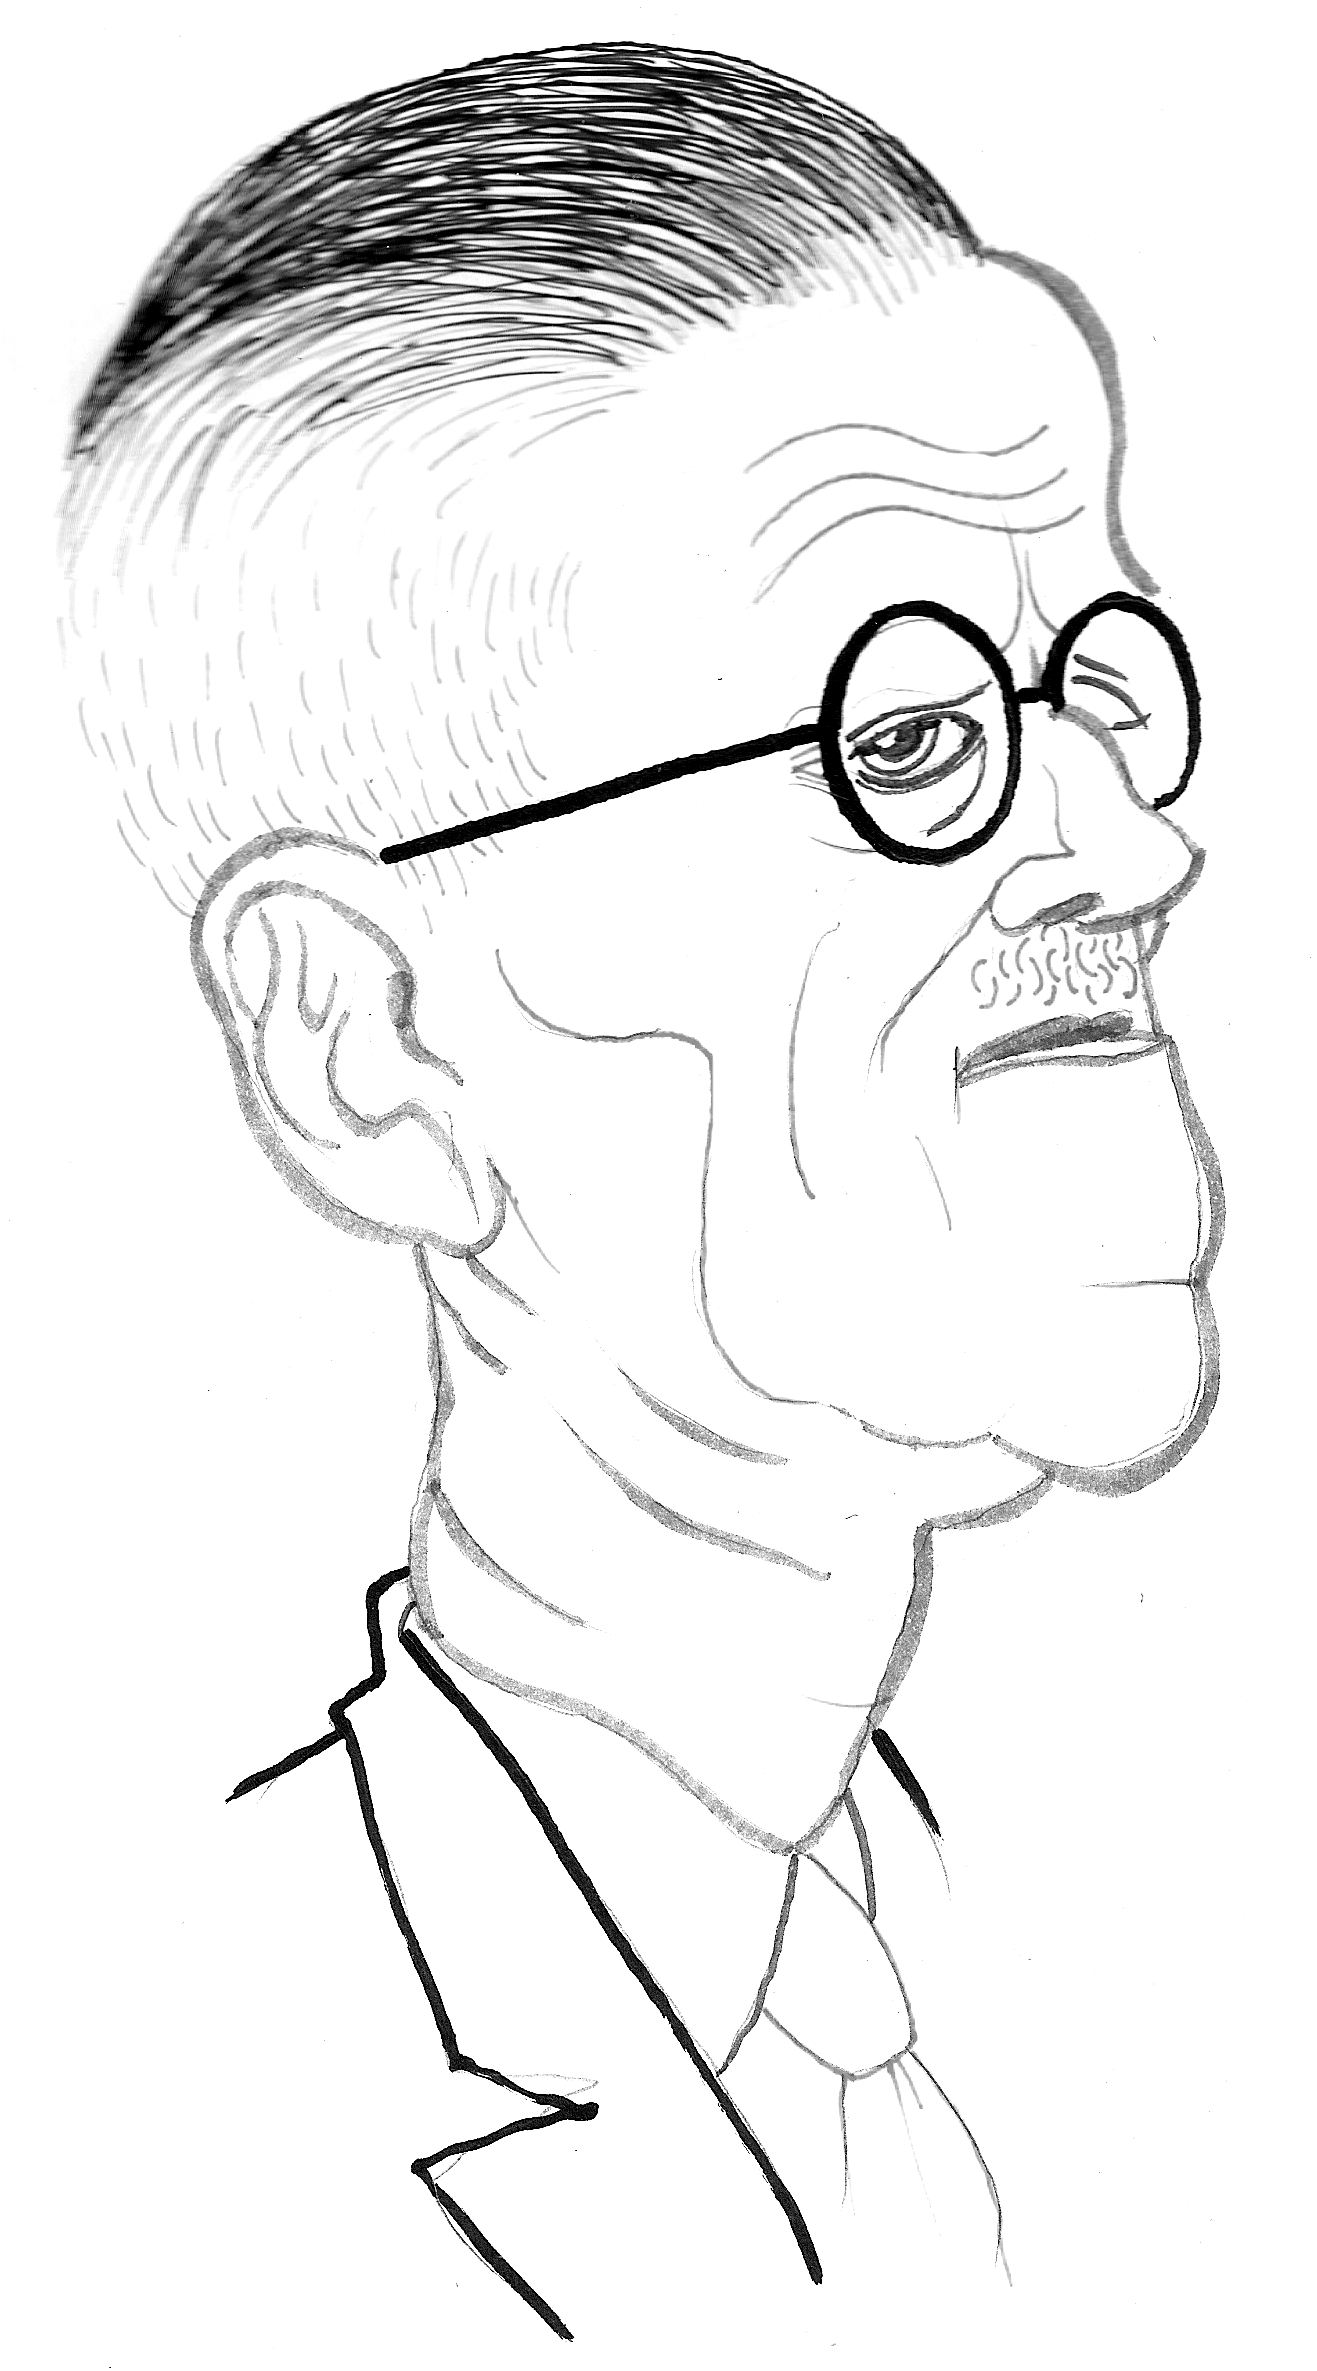
\includegraphics[width=.6\textwidth]{joyce5.jpg}
%\end{center}
%\vspace*{\fill}

\clearpage

\vspace*{.5\textheight}
\thispagestyle{empty}

\epigraph{Et ignotas animum dimittit in artes.\footnotemark}{\textsc{ovídio}, \textit{Metamorfoses}, \textsc{viii}, 188}
\footnotetext{“E ele aplica a mente às artes ocultas.”}

\chapter{\textsc{i}}

\textsc{Era uma vez,} galinha pedrês, uma vacamumu vindo pela estrada e a
vacamumu que vinha pela estrada encontrou um rapajinho bonjinho chamado
neném tuquim\ldots{}

O pai contava aquela história: o pai olhava para ele atrás de um vidro: 	
ele tinha o rosto peludo.

Ele era o neném tuquim. A vacamumu vinha pela estrada onde Betty Byrne
vivia: ela vendia palitinhos de limão.

\begin{verse}\itshape
\textit{Oh, a rosa selvagem floresce}\\
\textit{Lá no cantinho verde}.\footnote{ Trecho da balada
popular \textit{“Lily Dale”}. A letra correta é: “Agora a rosa selvagem floresce/ em sua sepulturinha verde”. [Todas as notas são do tradutor, exceto quando indicadas.]}
\end{verse}

Ele cantava essa canção. Ela era a canção dele.

\begin{verse}\itshape
\textit{Oh, a lója vêde foéche.}
\end{verse}

Quando a gente molha a cama, primeiro é morno, depois fica frio. E a mãe
punha o oleado. O com cheiro esquisito.

A mãe tinha um cheiro melhor que o pai. Ela tocava o \textit{sailor’s
hornpipe} no piano para ele dançar. Ele dançava:

\begin{verse}\itshape
\textit{Tralalá lalá}\\
\textit{Tralalá Tralalarí}\\
\textit{Tralalá lalá}\\
\textit{Tralalá lalá.}
\end{verse}

Tio Charles e a Tita batiam palmas. Eles eram mais velhos que o pai e a
mãe, mas tio Charles era mais velho que a Tita.

A Tita tinha duas escovas no armário. A escova com costas de veludo
marrom era para Michael Davitt e a escova com costas de veludo verde
era para Parnell.\footnote{ Michael Davitt e Charles Stewart Parnell,
políticos irlandeses, principais articuladores da campanha do
\textit{Home Rule}, pela autonomia política da Irlanda no Reino Unido.} A Tita lhe dava uma pastilha sempre que ele lhe
levava um lenço de papel.

Os Vance viviam no número sete. Eles tinham pai e mãe diferentes. Eles
eram o pai e a mãe de Eileen. Quando eles crescessem ele ia casar com
Eileen. Ele se escondeu debaixo da mesa. A mãe dele disse:

 --- Ah, o Stephen vai se desculpar.

A Tita disse:

 --- Ah, se não as águias vão pegar seus olhos e arrancar.


\begin{verse}\itshape
Pegar seus olhos e arrancar,\\
Se desculpar,\\
Se desculpar,\\
Pegar seus olhos e arrancar.

Se desculpar,\\
Pegar seus olhos e arrancar,\\
Pegar seus olhos e arrancar.\\
Se desculpar.
\end{verse}

Os vastos campos enxameavam de crianças. Todos gritavam e os prefeitos
os incentivavam aos berros. O ar da tarde era frio e pálido e depois de
cada investida e baque dos jogadores o orbe seboso de couro voava feito
um pássaro pesado na luz cinzenta. Ele se mantinha na fímbria da linha,
fora do alcance do prefeito, fora do alcance dos pés brutos, fingindo
correr de vez em quando. Sentia o corpo pequeno e fraco em meio ao
turbilhão dos jogadores e seus olhos eram fracos e aguados. Rody
Kickham não era assim: todo mundo dizia que ele seria o capitão da última turma.\footnote{ A
última turma era para crianças de até doze anos de idade. A segunda
turma era para meninos de treze a quinze anos, e a primeira, para rapazes de
dezesseis a dezoito.} 

Rody Kickham era um sujeito decente mas Nasty Roche era encrenqueiro.
Rody Kikcham tinha caneleiras no armário e comida só dele no
refeitório. Nasty Roche tinha mãos grandes. Ele chamava o prato de morcela de
sexta"-feira de “cachorro molhado”. E um dia perguntara:

 --- Qual o seu nome?

Stephen respondera:

 --- Stephen Dedalus.

Então Nasty Roche dissera:

 --- Que raio de nome é esse?

E quando Stephen não soube responder, Nasty Roche perguntara:

 --- Seu pai é o quê?

Stephen respondera:

 --- Um senhor.

Então Nasty Roche perguntara:

 --- Ele é juiz de paz?

Ele andava lentamente de um ponto a outro na fímbria da linha, dando
corridinhas às vezes. Mas suas mãos estavam azuis de frio. Ele mantinha
as mãos nos bolsos laterais do uniforme cinzento cintado. Aquilo em volta do bolso era um cinto
de couro. E couro também era dar um sopapo em
alguém. Um dia um colega dissera a Cantwell:

 --- Você ia entrar no couro rapidinho comigo.

Cantwell respondera:

 --- Vai lá jogar. Dá um couro em Cecil Thunder que eu quero ver. Ele vai
arregaçar você.

Essa não era uma expressão decente. A mãe o aconselhara a não falar com
os meninos brutos no colégio. A mãe era tão boa! No primeiro dia no
paço do castelo\footnote{ Onde fica instalado o Clongowes Wood
College.} ao dizer adeus ela subiu o véu até o nariz para beijá"-lo: e
os olhos e o nariz dela estavam vermelhos. Mas ele fingira não ter
notado que ela estava prestes a chorar. Ela era uma mãe tão boa, mas
não era tão boa quando chorava. E o pai dera a ele duas moedas de cinco
xelins para os gastos. E o pai dissera que qualquer coisa era só escrever
pra casa, e que ele nunca dedurasse um colega. Então na porta do
castelo o reitor apertara as mãos do pai e da mãe, sotaina sacudindo ao
vento, e a charrete partira levando o pai e a mãe. Eles o chamaram
da charrete, acenando:

 --- Adeus, Stephen, adeus!

 --- Adeus, Stephen, adeus!

Ele se viu no meio de uma disputa pela bola e, com medo dos olhos
faiscantes e das chuteiras enlameadas, se curvou para espiar por entre
as pernas. Os colegas lutavam e gemiam e suas pernas se esfregavam e
chutavam pisoteando o campo. Então as chuteiras amarelas de Jack Lawton
sacaram a bola e todas as outras chuteiras e pernas correram atrás
dela. Ele correu atrás deles um pouco e então parou. Era inútil correr
mais. Logo eles estariam indo passar as férias em casa. Depois da ceia
no salão de estudos ele mudaria o número colado dentro da carteira de
setenta e sete para setenta e seis.\footnote{ Número de dias até o final
do período.}

Seria melhor estar no salão de estudos do que ali fora, no frio. O céu
estava pálido e frio, mas havia luzes no castelo. Ele imaginou qual
teria sido a janela de onde Hamilton Rowan arremessara o chapéu no
fosso seco,\footnote{ Expediente pelo qual se diz que Archibald Hamilton
Rowan, membro da organização radical United Irishmen, teria conseguido 
escapar dos soldados britânicos que o estavam
perseguindo.} e será que havia canteiros de flores embaixo da janela
naquela época? Um dia ele foi chamado ao castelo e o mordomo lhe
mostrara as marcas das balas dos soldados na madeira da porta e lhe
dera um pedaço do bolo que a comunidade comia. Ver as luzes do castelo
era bom, dava um quentinho. Era como algo saído de um livro. Talvez a 
Abadia de Leicester fosse assim. E havia frases muito boas na Cartilha   
do Doutor Cornwell. Elas pareciam poesia, mas eram apenas frases para    
aprender a soletrar.

\begin{verse}\itshape
Wolsey morreu na Abadia de Leicester\\
Onde os abades o enterraram.\\
Cancro é doença de plantas,\\
Câncer é de animais.
\end{verse}

Seria bom ficar deitado no carpete em frente à lareira com a cabeça
apoiada nas mãos pensando nas frases. Ele se arrepiou como se água fria
e pegajosa tivesse lhe roçado a pele. Fora crueldade de Wells empurrá"-lo
na vala da latrina só porque ele não quis trocar sua caixinha de rapé
pela noz campeã de Wells, conquistadora de outras quarenta.\footnote{ No
jogo de \textit{conkers}, em que nozes amarradas a um fio são
arremessadas umas contra as outras até que apenas uma reste inteira.}
A água estava tão fria e pegajosa! Um aluno uma vez vira uma ratazana
gorda pular na espuma. A mãe estava sentada em frente à lareira com a
Tita esperando Brigid trazer o chá. Ela apoiava os pés no guarda"-fogo e
suas pantufas adornadas ficavam tão quentes, com um cheirinho morno tão
bom! A Tita sabia tanta coisa. Ela lhe ensinara onde ficava o
Canal de Moçambique e qual era o rio mais longo da América e qual era o
nome da montanha mais alta da Lua. O padre Arnall sabia mais coisas que
a Tita porque ele era padre, mas o pai e o tio Charles diziam que a
Tita era uma mulher inteligente e bastante lida. E quando a Tita fazia
aquele barulho depois do jantar e levava a mão à boca: aquilo se
chamava azia.

Uma voz gritou ao longe no campinho:

 --- Todos pra dentro!

E então outras vozes gritaram da última e da segunda turmas:

 --- Todos pra dentro! Todos pra dentro!

Os jogadores se aproximaram, afogueados e cobertos de lama, e ele foi
junto, feliz por poder entrar. Rody Kickham segurava a bola pelos
cordões sujos. Um aluno pediu pra ele dar um último chute: mas ele só
continuou caminhando e nem respondeu. Simon Moonan disse a ele pra não
fazer isso porque tinha um prefeito olhando. O colega se virou para
Simon Moonan e disse:

 --- A gente sabe por que você diz isso. Você é chupa"-ovo do McGlade.

Chupa era uma palavra esquisita. O aluno chamara Simon Moonan assim
porque Simon Moonan costumava brincar de amarrar as mangas falsas da
sotaina do prefeito atrás das costas e o prefeito fingia se
zangar.\footnote{ As sotainas dos professores tinham tiras de pano atrás
dos ombros.} Mas o som era feio. Uma vez ele lavara as mãos no
banheiro do Hotel Wicklow e o pai puxara a rolha pela correntinha
e a água suja escorrera pelo buraco da pia. E quando tudo tinha
escorrido o buraco da pia fez um som assim: \textit{chupa}. Mas mais
alto.

Lembrar aquilo e a aparência branca do banheiro o fez sentir frio e
depois calor. Havia duas torneiras que a gente girava para água sair:
fria e quente. Ele sentiu frio e um pouco de calor: e ele podia ver os
nomes impressos nas torneiras. Aquilo era muito esquisito.

E o ar no corredor também o enregelava. Era esquisito e molhado. Mas
logo o gás era aceso, e ao queimar fazia um barulhinho assim como uma
cançãozinha. Sempre igual: e quando os alunos paravam de falar na sala
de jogos dava para ouvir.

Era a hora das contas. Padre Arnall escreveu uma conta difícil no quadro
e disse:

 --- E agora, quem vai ganhar? Vamos lá, York! Vamos lá,
Lancaster!\footnote{ As duas dinastias envolvidas na Guerra das Rosas
(1445--85). Padre Arnall dividia a turma em dois times, um representando
a casa de York (com a rosa branca), e o outro, a casa de Lancaster (a
rosa vermelha).}

Stephen fez o que pôde, mas a conta era muito difícil e ele se sentia
confuso. O pequeno emblema de seda com a rosa branca afixado em sua
lapela começou a tremer. Ele não era bom em contas, mas deu o melhor de
si para que York não perdesse. O rosto do padre Arnall estava escuro, 
mas ele não estava com raiva: ele estava rindo. Então Jack Lawton
estalou os dedos e o padre Arnall olhou em seu caderno e disse:

 --- Está certo. Bravo, Lancaster! A rosa vermelha vence. Vamos lá, York!
Adiante!

Jack Lawton olhou por cima do ombro. O pequeno emblema de seda com a
rosa vermelha lhe caía bem, pois ele usava um colete azul de
marinheiro. Stephen sentiu o próprio rosto vermelho também, ao pensar
em todas as apostas sendo feitas sobre quem ficaria em primeiro nos
estudos, Jack Lawton ou ele. Em algumas semanas era Jack Lawton quem
obtinha o cartão de primeiro lugar, em outras era ele quem obtinha o
cartão de primeiro lugar. O emblema branco de seda tremia e tremia
enquanto ele trabalhava na próxima conta, ouvindo a voz do padre
Arnall. Então toda a pressa sumiu e ele sentiu o rosto ficar frio. Ele
pensou que seu rosto devia estar branco de tanto frio que sentia. Ele
não conseguiu encontrar a resposta para a conta, mas não importava. Rosas
brancas e rosas vermelhas: cores bonitas para a gente matutar. E os 
cartões de primeiro e segundo e terceiro lugar também tinham cores
bonitas: rosa e bege e lavanda. Rosas beges, cor"-de"-rosa e lavanda eram
bonitas de se imaginar. Talvez uma rosa selvagem tivesse cores assim e
ele se lembrou da canção sobre botões de rosa selvagem lá num cantinho
verde. Mas não existiam rosas verdes. Mas talvez em algum lugar do
mundo existissem.

O sino tocou e as turmas saíram em fila das salas e seguiram pelos
corredores até o refeitório. Ele ficou sentado olhando os dois
montinhos de manteiga no prato, mas não pôde comer o pão úmido. A
toalha de mesa estava úmida e molenga. Mas ele bebeu o chá fraco e
quente que o ajudante desajeitado de avental branco despejou em seu
copo. Ele se perguntou se o avental do ajudante estava úmido também, ou
se todas as coisas brancas eram frias e úmidas. Nasty Roche e Saurin
bebiam o chocolate em lata enviado pelos pais. Eles diziam que não
conseguiam beber o chá; que era lavagem. O pessoal dizia que os pais
deles eram juízes de paz.

Todos os garotos pareciam"-lhe muito estranhos. Todos eles tinham pais e
mães e roupas e vozes diferentes. Ele ansiava por estar em casa e
repousar a cabeça no colo da mãe. Mas ele não podia: e assim ele ansiou
pelo fim dos jogos e estudos e preces para poder ir pra cama. 

Ele bebeu outro copo do chá quente e Fleming disse:

 --- Qual o problema? Você está sentindo dor, qual o problema?

 --- Eu não sei --- Stephen disse.

 --- Isso é enjoo --- Fleming disse ---, sua cara tá toda branca. Já já passa.

 --- Ah é --- Stephen disse.

Mas ele não estava enjoado, não no estômago. Ele pensou que devia estar
enjoado no coração, se é que algo assim existia. Fleming era bem bacana
por perguntar. Ele queria chorar. Ele apoiou os cotovelos na mesa e
abriu e fechou as abas das orelhas. Então ele ouviu os barulhos do
refeitório cada vez que abria as orelhas. Rugia feito um trem à noite.
E ao fechar as abas o rugido cessava como se o trem entrasse em um
túnel. Naquela noite em Dalkey o trem rugira assim, e ao entrar no
túnel o rugido cessara. Ele fechou os olhos e o trem continuou, rugindo
e parando; rugindo e parando. Era bom ouvir o trem rugir e parar e
depois rugir saindo do túnel de novo e então parar.

Então os alunos da primeira turma começaram a vir pelo capacho no meio
do refeitório, Paddy Rath e Jimmy Magee e o espanhol que podia fumar
charutos e o portuguesinho com o boné de lã. E então as mesas da
segunda turma e as mesas da última turma. E cada um dos alunos andava
diferente.

Ele sentou em um canto da sala de jogos fingindo assistir a uma partida
de dominó e uma ou duas vezes ele ouviu por um instante a cançãozinha
do gás. O prefeito estava à porta com alguns garotos e Simon Moonan
estava amarrando suas mangas falsas. Simon Moonan estava contando aos
garotos algo sobre Tullabeg.\footnote{ Antiga sede dos jesuítas na
Irlanda.}

Então ele se afastou da porta e Wells veio até Stephen e disse:

 --- Ei, Dedalus, fala pra gente, você beija sua mãe antes de dormir?

Stephen respondeu:

 --- Sim.

Wells se virou para os outros garotos e disse:

 --- Ih, olha só, este sujeito aqui falou que beija a mãe toda noite antes
de dormir.

Os outros garotos pararam de jogar e se viraram, rindo. Stephen corou e
disse:

 --- Não beijo.

Wells disse:

 --- Ih, olha só, ele falou que não beija a mãe toda noite antes de ir
dormir.

Todos riram novamente. Stephen tentou rir com eles. Subitamente ele
sentiu o corpo inteiro quente e confuso. Qual era a resposta certa para
a pergunta? Ele respondera duas vezes e Wells rira igual. Mas Wells
devia saber a resposta certa, pois ele estava no terceiro ano de
gramática. Ele tentou pensar na mãe de Wells, mas não ousou erguer os
olhos até o rosto dele. Ele não gostava do rosto de Wells. Fora Wells
quem o empurrara na vala no dia anterior porque ele não quis trocar sua
caixinha de rapé pela noz campeã de Wells, conquistadora de outras quarenta. 
Uma coisa cruel de se fazer; todo mundo disse isso. E a água
era tão fria e pegajosa! E um aluno uma vez vira uma ratazana gorda
pular em cheio na espuma.

O limo frio da vala cobria todo o seu corpo; e quando o sino tocou para as
aulas e os alunos saíram em fila das salas de recreação ele sentiu o ar
frio do corredor e da escadaria dentro das roupas. Ele ainda tentou
descobrir qual seria a resposta certa. Era certo beijar a mãe ou era
errado beijar a mãe? O que significava beijar? A gente levanta o rosto
assim para dizer boa"-noite e então a mãe inclinava o rosto. Isso era 
beijar. A mãe pousava os lábios na bochecha dele; os lábios dela eram
macios e molhavam sua bochecha; e faziam um barulhinho: \textit{b'ij}.
Por que as pessoas faziam isso com o rosto delas?

Sentado na sala de estudos ele abriu a tampa da carteira e mudou o
número colado ali de setenta e sete para setenta e seis. Mas as férias
de Natal estavam muito longe: mas um dia chegariam, porque a Terra
nunca parava de girar.

Havia uma imagem da Terra na primeira página do livro de geografia: uma
bola grande no meio das nuvens. Fleming tinha uma caixa de lápis de
cor, e uma noite durante o período de estudo livre ele pintara a Terra
de verde e as nuvens de marrom. Que nem as escovas no armário da Tita,
a escova com as costas de veludo verde para Parnell e a escova com as
costas de veludo marrom para Michael Davitt. Mas ele não dissera a
Fleming que as pintasse naquelas cores. Fleming fizera aquilo sozinho.

Ele abriu o livro de geografia para estudar a lição; mas não conseguia
decorar os nomes dos lugares na América. Mas eram todos lugares
diferentes, com nomes diferentes. Eles ficavam em países diferentes e
os países ficavam em continentes e os continentes ficavam no mundo e o
mundo ficava no universo.

Ele se voltou para a primeira página do livro de geografia e leu o que
escrevera ali: ele próprio, seu nome e onde estava.

\begin{verse}\itshape
Stephen Dedalus\\
Classe Elementar\\
Clongowes Wood College\\
Sallins\\
County Kildare\\
Irlanda\\
Europa\\
O Mundo\\
O Universo
\end{verse}

Ele escrevera aquilo: e Fleming, para fazer graça, uma noite escrevera na
página oposta:

\begin{verse}\itshape
Stephen Dedalus é meu nome.\\
Clongowes é onde estou morando,\\
Mas a Irlanda é minha nação\\
E o céu está me esperando.
\end{verse}

Ele leu as linhas de trás para frente, mas aí elas já não eram poesia.
Então leu a primeira página de baixo para cima até chegar ao próprio
nome. Aquele era ele: e ele leu a página até embaixo de novo. O que
havia depois do Universo? Nada. Mas havia alguma coisa ao redor do
Universo para mostrar onde o Universo terminava e o lugar do nada
começava? Não devia ser uma parede, mas podia haver uma linha fina ao
redor de tudo. Era enorme demais pensar em tudo em toda parte. Só Deus
conseguia fazer isso. Ele tentou imaginar o quão grande era esse
pensamento, mas só conseguiu pensar em Deus. Deus era o nome de Deus,
assim como Stephen era o seu nome. \textit{Dieu} era Deus em francês, e
era o nome de Deus também; e quando alguém rezava para Deus e dizia
\textit{Dieu}, Deus sabia na hora que a pessoa rezando era
francesa. Mas embora houvesse diferentes nomes para Deus em todas as
línguas diferentes do mundo e embora Deus entendesse o que as pessoas
todas diziam rezando em línguas diferentes, Deus continuava sendo o
mesmo Deus e o nome de verdade de Deus era Deus.

Pensar assim o deixava muito cansado. Fazia com que ele sentisse a
cabeça enorme. Ele virou a primeira página e olhou cansado para a Terra
redonda e verde no meio das nuvens marrons. Ele se perguntou qual seria
o certo, torcer pelo verde ou pelo marrom, porque um dia a Tita
arrancara o veludo verde das costas da escova de Parnell e lhe dissera
que Parnell era um homem mau. Ele se perguntou se em casa eles estariam
discutindo aquilo. O nome daquilo era política. Havia dois lados nela:
a Tita estava de um lado e o pai e o sr.~Casey estavam do outro lado
mas a mãe e o tio Charles não estavam em lado nenhum. Todo dia havia
algo no jornal sobre aquilo.

Doía"-lhe o fato de ele não saber direito o que era política, nem onde o
Universo terminava. Ele se sentiu pequeno e fraco. Quando é que ele
ficaria igual aos alunos de Poesia e Retórica? Eles tinham vozes altas,
botas grandes e estudavam trigonometria. Isso ainda estava longe.
Primeiro vinham as férias e depois o outro período e então férias de
novo e então outro período e depois as férias. Era como um trem
entrando e saindo de túneis, que era como o barulho dos garotos comendo
no refeitório quando a gente fechava e abria as abas das orelhas.
Período, férias; túnel, fora; barulho, parada. Ainda estava tão longe!
Era melhor ir para a cama dormir. Só faltava rezar na capela, e então
cama. Ele tremeu e bocejou. A cama ficaria ótima depois que os lençóis
esquentassem um pouquinho. Eles eram tão frios no início. Ele se
arrepiou lembrando do quão frios eles eram. Mas aí eles esquentavam e
ele conseguia dormir. Era gostoso estar cansado. Ele bocejou de novo.
Orações noturnas e cama: ele se arrepiou e quis bocejar. Em alguns
minutos estaria bem gostoso. Ele sentiu um brilho tépido subindo dos
lençóis friorentos, mais e mais morno até ele ficar todo quente dos
pés à cabeça, e ainda então ele se arrepiou um pouco e mais uma vez
quis bocejar.

O sino tocou para as orações noturnas e ele saiu do salão de estudos
depois dos outros e desceu a escadaria passando pelos corredores até a
capela. Os corredores eram mal iluminados e a capela era mal iluminada.
Logo tudo seria escuridão e sono. Havia ar frio da noite na capela e os
mármores estavam da cor do mar à noite. O mar era frio noite e dia: mas
era mais frio à noite. Era frio e escuro debaixo do quebra"-mar do lado
da casa do pai. Mas a chaleira estaria atrás da lareira, pronta para o
\textit{punch}.                                                        

O prefeito da capela rezava acima de sua cabeça e sua memória conhecia
as respostas:

\begin{verse}\itshape
Abre, Senhor, nossos lábios\\
E nossas bocas proclamarão o Teu louvor.\\
Inclina"-Te à nossa ajuda, Oh Deus!\\
Ó Senhor, apressa"-Te em nos socorrer!
\end{verse}

Havia um cheiro frio de noite na capela. Mas era um cheiro santo. Não
era como o cheiro dos velhos camponeses ajoelhados nos fundos da capela
na missa de domingo. Aquele era um cheiro de ar e chuva e turfa e
veludo. Mas eles eram camponeses muito santos. Eles respiravam em sua
nuca e suspiravam ao rezar. Eles viviam em Clane, um colega disse:
havia pequenas cabanas lá e ele vira uma mulher em pé à meia"-porta de
uma cabana com uma criança nos braços quando ele veio de Sallins de
charrete. Seria tão bom dormir por uma noite naquela cabana diante do
fogo de turfa fumegante, no fogo, no breu morno, sentindo o cheiro dos
camponeses, do ar, da chuva e do veludo. Mas, ah, a estrada pra lá
entre as árvores era escura! A gente se perderia no escuro. Pensar em
se perder o deixava com muito medo.

Ele ouviu a voz do prefeito da capela dizendo as últimas preces. Ele
também orou contra a escuridão do lado de fora embaixo das árvores.

\begin{quote}
Visita, Oh Senhor, este lar, nós Te rogamos, e expulsa dele todas as
armadilhas do inimigo. Que Teus anjos sagrados aqui fiquem nos
guardando na paz e que Tua bênção esteja sempre conosco por meio de
Cristo nosso Senhor, Amém.

\end{quote}
Seus dedos tremiam enquanto ele se despia no dormitório. Ele disse para os
dedos se apressarem. Ele tinha que se despir e então se ajoelhar e
dizer as orações e cair na cama antes de apagarem o gás ou ele iria
para o inferno quando morresse. Ele tirou as meias enrolando"-as e
vestiu o camisolão rapidamente e se ajoelhou tremendo ao lado da cama e
repetiu as preces depressa, temendo que o gás se apagasse. Ele sentiu os
ombros tremendo enquanto murmurava:

\begin{verse}\itshape
Deus abençoe meu pai e minha mãe e os conserve!\\
Deus abençoe minhas irmãs e irmãos pequenos e os conserve!\\
Deus abençoe a Tita e o tio Charles e os conserve!
\end{verse}

Ele se persignou e pulou rápido na cama e, enfiando a barra do camisolão
debaixo dos pés, se enrolou debaixo dos lençóis brancos e frios,
tremendo e sacudindo. Mas ele não iria para o inferno quando morresse;
e o tremor pararia. Uma voz deu boa"-noite aos garotos no dormitório.
Ele espiou um instante por cima das cobertas e viu as cortinas amarelas
ao redor e à frente da cama, isolando"-o de todos os lados. A luz foi se
apagando lentamente.

Os sapatos do prefeito se afastaram. Para onde? Desceram a escadaria e
seguiram pelos corredores ou foram para o quarto dele, lá do outro
lado? Ele viu a escuridão. Era verdade a história sobre o cão negro que
caminhava à noite com olhos grandes como faróis de charrete? Diziam que
era o fantasma de um assassino. Um longo arrepio de medo perpassou
seu corpo. Ele viu o saguão de entrada escuro do castelo. Antigos
serviçais em roupas antigas estavam na sala de armas acima da
escadaria. Era há muito tempo. Os antigos serviçais estavam quietos.
Havia um fogo aceso lá, mas o saguão ainda estava escuro. Um vulto
subiu a escadaria, vindo do saguão. Ele usava um manto branco de
marechal e seu rosto era pálido e estranho. Ele mantinha a mão junto ao
flanco. Ele olhava através de olhos estranhos para os antigos
serviçais. Eles olharam para ele e viram o rosto e o manto do amo e
souberam que ele havia sido ferido de morte. Mas no ponto para onde
olhavam só havia breu: apenas ar escuro e silente. O amo havia sido
ferido de morte no campo de batalha de Praga, bem longe, no além"-mar.
Ele estava de pé no campo, a mão junto ao flanco. Seu rosto era pálido
e estranho e ele usava o manto branco de um marechal.

Ah, quão frio e estranho era pensar em tudo aquilo! E todo o breu era
frio e estranho. Havia estranhas faces pálidas ali, grandes olhos como
faróis de charrete. Eles eram os fantasmas de assassinos, os vultos de
marechais feridos de morte em campos de batalha bem longe, no além"-mar.
O que eles queriam dizer que tornava seus rostos tão estranhos?

\begin{quote}
Visita, Oh Senhor, este lar, nós Te rogamos, e expulsa dele
todas\ldots{}

\end{quote}
Ir pra casa nas férias! Seria tão bom: os colegas lhe disseram. Subir
nas charretes cedo na manhã de inverno fora do castelo. As charretes
deslizavam no cascalho. Vivas para o reitor!

Viva! Viva! Viva!

As charretes passaram pela capela e os bonés se levantaram. Eles
seguiram alegres pelas estradas do interior. Os condutores apontavam
com os chicotes para Bodenstown. Os colegas deram vivas. Eles passaram
pela fazenda do Fazendeiro Feliz. Vivas e vivas e vivas. Foram por
Clane, saudando e sendo saudados. As camponesas estavam em pé diante
das meias"-portas, os homens espalhados aqui e ali. O cheiro bom de lá
pairava no ar de inverno: o cheiro de Clane: chuva e ar de inverno e
turfa fumegante e veludo.

O trem ia cheio de colegas: um trem grande cor de chocolate, grande e
com os lados cor de creme. Os guardas iam e vinham, abrindo e fechando
e trancando e destrancando as portas. Eles eram homens vestindo azul
escuro e prata; tinham apitos prateados e levavam chaves que produziam
música ligeira: clique clique: clique clique.

E o trem seguiu pelas planícies, passando pela Colina de Allen. Os
postes telegráficos passavam, passavam. O trem seguia e seguia. Ele
sabia. Havia lanternas no salão da casa paterna e cordas feitas de
ramas verdes. Havia azevinho e hera emoldurando o grande espelho, e
azevinho e hera, verde e vermelha, entretecidos ao redor dos lustres.
Havia azevinho vermelho e hera verde ao redor dos antigos retratos nas
paredes. Azevinho e hera por causa dele e do Natal.

Tão bom\ldots{}

Todo mundo. Bem"-vindo ao lar, Stephen! Ruídos de boas"-vindas. A mãe o
beijou. Aquilo era certo? O pai agora era marechal: mais que juiz de
paz. Bem"-vindo ao lar, Stephen!

Ruídos\ldots{}

Houve um ruído de argolas de cortinas deslizando nos paus, de água
derramada em terrinas. Houve ruído de levantar e se vestir e se lavar
no dormitório: barulho de palmas enquanto o prefeito ia para cima e
para baixo mandando os colegas se aprontarem. A luz do sol desmaiada
mostrava as cortinas amarelas repuxadas, as camas desarrumadas. Sua
cama estava muito quente e seu corpo e rosto estavam muito quentes.

Ele se levantou e sentou na beirada da cama. Ele se sentia fraco. Tentou
calçar uma meia. Tinha uma textura áspera horrenda. A luz do sol estava
fria e esquisita.

Fleming disse:

 --- Não está se sentindo bem?

Ele não sabia; e Fleming disse:

 --- Volte pra cama. Eu digo pro McGlade que você não está se sentindo bem.

 --- Ele está doente.

 --- Quem?

 --- Vá dizer pro McGlade.

 --- Volte pra cama.

 --- Ele está doente?

Um colega segurou seus braços enquanto ele se livrava da meia ainda
presa ao pé e voltava para cama quente.

Ele se agachou entre os lençóis, feliz com o brilho morno que emanava
deles. Ouviu os colegas comentando entre si a seu respeito ao se
vestirem para a missa. Fora muita crueldade empurrá"-lo na vala, eles
diziam.

Então as vozes pararam; tinham"-se ido. Uma voz na cama lhe disse:

 --- Dedalus, não me dedura não, tá legal?

O rosto de Wells estava ali. Ele olhou e viu que Wells estava com medo.

 --- Não fiz por mal. Não conta nada?

O pai lhe dissera que, não importa o que acontecesse, ele não deveria
dedurar um colega. Ele sacudiu a cabeça e respondeu não e se sentiu
feliz.

Wells disse:

 --- Eu não fiz por mal, palavra. Foi de brincadeira. Desculpa.

O rosto e a voz sumiram. Ficou com pena, pois o outro tinha medo. Medo
de que fosse alguma doença. Cancro era doença de plantas, e câncer, de
animais: ou alguma outra. Aquilo fora há muito tempo lá fora nos campos
à luz da noite, indo devagar de ponta a ponta na fímbria da linha, um
pássaro pesado voando baixo na luz cinzenta. Leicester Abbey acesa.
Wolsey morrera lá. Os próprios abades o enterraram.

Não era o rosto de Wells, era o rosto do prefeito. Ele não estava
fingindo. Não, não: ele estava doente mesmo. Ele não estava fingindo. E
ele sentiu a mão do prefeito em sua testa; e ele sentiu a testa quente
e úmida contra a mão fria e úmida do prefeito. Era assim que um rato se
sentia, viscoso e úmido e frio. Todo rato tinha dois olhos por onde
olhar. E pelo viscoso e lambido, pés pequenos, pequeninos, prontos para
pular e olhos negros viscosos por onde espiar. Eles entendiam pular.
Mas as mentes dos ratos não entendiam trigonometria. Ao morrer, eles
viravam de lado. O pelo deles secava. E então eles eram apenas coisas
mortas.

O prefeito estava lá de novo e era a voz dele que lhe dizia para se
levantar, que o padre ministro dissera para ele se levantar e se vestir 
e ir para a enfermaria. E enquanto ele se vestia o mais rápido que podia,
o prefeito disse:

--- Temos que ir visitar o irmão Michael porque estamos com nó nas
tripas! Mas que tristeza, nó nas tripas! Eita nós com nós nas tripas!

Ele era bacana dizendo aquilo para fazê"-lo rir. Mas ele não conseguia rir
porque suas bochechas e lábios estavam trêmulos: e o prefeito teve que
rir sozinho.

O prefeito falou alto:

 --- Marcha puxada! Esquerda! Direita!

Eles desceram juntos pela escadaria e pelo corredor, passando pelos
lavatórios. Ao passar pela porta ele lembrou com um medo vago a água
suja cor de turfa, o ar úmido e morno, o som de mergulhos, o cheiro das
toalhas, feito remédio.

O irmão Michael estava em pé à porta da enfermaria e da porta do armário
escuro à sua direita vinha o cheiro de remédio. Que vinha das garrafas nas
prateleiras. O prefeito falou com o irmão Michael e o irmão Michael
respondeu, chamando o prefeito de senhor. Ele tinha cabelo vermelho e
grisalho e um jeito esquisito. Era esquisito ele ser pra sempre um
irmão. Era esquisito a gente não poder chamá"-lo de senhor porque ele
era um irmão e ele tinha um jeito assim diferente. Será que ele não era
santo o suficiente, ou então por que é que ele não acompanhava os
outros?\footnote{ O irmão Michael era coadjutor temporal da Companhia de
Jesus, uma função para a qual não era necessário ter a rigorosa
educação jesuítica exigida para os frades. Sob sua responsabilidade
ficavam tarefas domésticas como serviços de limpeza, cozinha etc.}

Havia duas camas no cômodo e em uma delas se sentava um colega: e quando
entraram ele chamou:

 --- Ei! É o Dedalus! Tudo em cima?

 --- Só o céu --- disse o irmão Michael.

Ele estava no terceiro ano de gramática e, enquanto Stephen se despia,
ele pediu ao irmão Michael que lhe trouxesse torradas amanteigadas.

 --- Por favor! --- ele disse.

 --- Eu passo você na manteiga já já! --- disse o irmão Michael. --- Você vai ter alta pela manhã, quando o doutor chegar.

 --- Vou, é? --- o colega disse. --- Eu ainda não estou bom.

O irmão Michael repetiu:

 --- Você vai ter alta, estou dizendo.

Ele se agachou para atiçar o fogo, mostrando as costas, longas como as de
um cavalo puxador de bonde. Ele sacudiu o atiçador, sério, e acenou com
a cabeça para o colega do terceiro ano de gramática.

Então o irmão Michael saiu, e depois de um tempo o colega do terceiro
ano de gramática se virou para a parede e dormiu.

Aquela era a enfermaria. Então ele estava doente. Será que eles tinham
escrito para a casa dele para avisar ao pai e a mãe? Mas seria mais
rápido um dos frades ir pessoalmente contar para eles. Ou ele podia
escrever uma carta para o frade levar.

\smallskip

Querida Mamãe,

Estou doente. Quero ir pra casa. Por favor, venha me buscar. Estou na
enfermaria.

{\raggedleft
Seu querido filho,\\
Stephen.
\par}

\smallskip

Mas eles estavam tão longe! A luz do sol parecia fria lá fora. Ele se
perguntou se iria morrer. Para morrer qualquer dia serve, mesmo se for
um dia ensolarado. Ele podia morrer antes da mãe chegar. Daí ele teria
uma missa de corpo presente na capela, que nem os colegas disseram que
Little teve quando morreu. Todos os colegas estariam na missa, vestidos
de preto, todos com rostos tristes. Wells estaria lá também, mas nenhum
colega olharia para ele. O reitor estaria lá com um pluvial negro e
dourado e haveria grandes velas amarelas no altar e ao redor do
catafalco. E eles carregariam lentamente o caixão para fora da igreja
para ser enterrado no pequeno cemitério da comunidade, depois da
avenida principal de tílias. E Wells se sentiria culpado pelo que tinha
feito. E o sino plangeria lentamente.

Ele podia ouvir o som dos sinos. Ele repetiu para si mesmo a canção que
Brigid havia lhe ensinado.

\begin{verse}\itshape
Blém"-blém! O sino do castelo!\\
Adeus, minha mãezinha!\\
Me enterrem no velho adro,\\
Do meu irmão mais velho ao lado.\\
Meu caixão vai ser bem preto,\\
Com seis anjos me guardando,\\
Dois cantando, dois rezando\\
E dois minh’alma arrebatando.
\end{verse}

Era tão lindo e triste! Que lindas eram as palavras na parte do
\textit{Me enterrem no velho adro}! Um tremor percorreu seu corpo. Era
tão triste e lindo! Ele quis chorar baixinho, mas não por causa dele:
pelas palavras, tão lindas e tristes, feito música. O sino! O sino!
Adeus! Oh, adeus!

A fria luz do sol caía mais fraca e o irmão Michael estava em pé ao seu
lado com uma tigela de caldo de carne. Ele ficou feliz, pois tinha a
boca quente e seca. Ele podia ouvir os colegas jogando no campinho.  E
o dia prosseguia na escola sem ele, do mesmo jeito.

Então o irmão Michael se voltou para sair e o colega do terceiro ano de
gramática lhe disse para voltar depois e lhe contar as notícias do
jornal. Ele disse a Stephen que seu nome era Athy e que seu pai tinha
muitos cavalos de corrida saltadores bem treinados, e que o pai daria
uma boa gorjeta ao irmão Michael sempre que ele quisesse, pois o irmão
Michael era muito bacana e sempre lia as notícias do jornal que chegava
ao castelo todo dia. Havia todo tipo de notícia no jornal: acidentes,
naufrágios, esportes e política.

 --- Agora tudo é política no jornal --- ele disse. --- O seu pessoal fala disso também?

 --- Sim --- Stephen disse.

 --- O meu também --- ele disse.

Então, depois de pensar um pouco, ele disse:

 --- Você tem um nome esquisito, Dedalus, e eu tenho um nome esquisito
também. Athy. Meu nome é o nome de uma cidade. E o seu nome parece
latim.

Então ele perguntou:

 --- Você é bom com charadas?

Stephen respondeu:

 --- Não sou muito não.

Então ele disse:

 --- Você consegue responder esta?  Por que o condado de Kildare é igual a
uma perna de calça?

Stephen pensou em qual poderia ser a resposta e então disse:

 --- Desisto.

 --- Porque os dois têm uma coxa\footnote{ Trocadilho intraduzível entre
\textit{Athy} (o nome da cidade) e \textit{a thigh} (uma coxa).} ---
ele disse. --- Entendeu? Athy é uma cidade no condado de Kildare.

 --- Ah, entendi --- Stephen disse.

 --- Essa charada é velha --- ele disse.

Depois de um momento disse:

 --- Olha só!

 --- O quê? --- Stephen perguntou.

 --- Sabe --- ele disse ---, dá pra fazer essa charada de outro jeito.

 --- Dá? --- Stephen disse.

 --- A mesma charada --- ele disse. --- Você sabe o outro jeito de fazer?

 --- Não --- Stephen disse.

 --- Não consegue pensar em outro jeito? --- ele disse.

Ele olhou para Stephen por cima dos lençóis enquanto falava. Então ele
se recostou no travesseiro e disse:

 --- Tem outro jeito, mas eu não vou dizer.

Por que ele não disse? O pai dele, que tinha cavalos de corrida, devia
ser juiz de paz que nem o pai de Saurin e o pai de Nasty Roche. Ele pensou no
próprio pai, como ele cantava enquanto a mãe tocava e como ele sempre
lhe dava um xelim quando ele pedia seis \textit{pence} e ele se sentiu
mal por seu pai não ser juiz de paz feito o pai dos outros garotos. Então por que
ele fora enviado para aquele lugar com os outros garotos? Mas seu pai
lhe dissera que ele não seria mal recebido ali, pois seu tio"-avô havia
discursado nas boas"-vindas ao Libertador\footnote{ Daniel O’Connell
(1775--1847). Obteve a emancipação católica na Irlanda.} lá, há
cinquenta anos. Dava pra reconhecer o povo daquela época pelas roupas. 
Aquela lhe parecia uma época solene: e ele se perguntava se aquela fora
a época em que os colegas de Clongowes usavam casacos azuis com botões
de latão, coletes amarelos e chapéus de pele de coelho, quando eles
bebiam cerveja como gente grande e tinham sabujos para caçar lebres.

Ele olhou pela janela e viu a luz do dia já mais fraca. Sobre os campos
agora haveria uma luz cinzenta e enevoada. Não havia barulho no
campinho. As turmas deviam estar fazendo redação ou talvez padre Arnall
estivesse contando a história da vida de algum santo.

Era esquisito não terem lhe dado remédio. Talvez o irmão Michael
trouxesse quando voltasse. Eles diziam que na enfermaria davam coisas
fedidas para a gente beber. Mas ele se sentia melhor agora. Era bom ir 
ficando bom aos pouquinhos. A gente ganhava um livro. Tinha um livro na
biblioteca sobre a Holanda. Havia lindos nomes estrangeiros nele e
imagens de cidades e navios de aparência estranha. Fazia a gente se
sentir tão feliz.

A luz na janela era tão pálida! Mas era bom. O fogo se levantava e caía
na parede. Que nem ondas. Alguém tinha posto carvão e ele ouvira vozes.
Estavam falando. Era o barulho das ondas. Ou eram as ondas conversando
enquanto se levantavam e caíam.

Ele viu o mar de ondas, longas ondas negras se erguendo e caindo escuras
numa noite sem luar. Uma luzinha piscava no atracadouro para onde seguia
o navio: e ele viu uma multidão reunida à beira d’água
para ver o navio que chegava ao atracadouro. Um homem alto estava no
convés, encarando a terra escura e plana: e pela luz no atracadouro
Stephen viu o rosto do homem, o rosto triste do irmão Michael.

Ele o viu levantar as mãos para o povo e o ouviu dizer em uma voz alta,
cheia de tristeza, por sobre as águas:

 --- Ele morreu. Nós o vimos prostrado no catafalco. 

Um gemido de dor se ergueu da multidão.

 --- Parnell! Parnell! Ele morreu!

Eles caíram de joelhos, gemendo de dor e mágoa.

E ele viu a Tita em um vestido de veludo marrom e com um xale de veludo
verde nos ombros caminhando orgulhosa e silenciosamente entre as
pessoas ajoelhadas à beira d’água.

\medskip

Um grande fogo insuflado alto e rubro crepitava no gradil, e sob o lustre
com as gavinhas de hera entretecidas a mesa de Natal foi arrumada. Eles
chegaram em casa um pouco tarde e o jantar ainda não estava
pronto: mas estaria pronto num pulinho, a mãe dissera. Eles esperavam
que a porta se abrisse para os serviçais entrarem, segurando os grandes
pratos cobertos com as tampas de metal pesado.

Todos esperavam: tio Charles, sentado mais distante à sombra da janela,
a Tita e o sr.~Casey, sentados nas poltronas dos dois lados da lareira, 
Stephen, sentado em uma cadeira entre eles e com os pés descansando no
pufe aquecido. O sr.~Dedalus se mirou no espelho alto acima do lintel
da lareira, aguçou as pontas do bigode com os dedos e então, afastando
as abas do fraque, ficou de costas para o fogo: e de vez em quando ele
soltava uma das caudas do fraque para aguçar as pontas do bigode. O sr.~Casey 
inclinou a cabeça para o lado e, sorrindo, deu tapinhas de leve
com os dedos no pomo de adão. E Stephen também sorriu, pois agora ele
já sabia que não era verdade que o sr.~Casey tinha uma bolsa de moedas
na garganta. Ele sorriu pensando em como fora enganado pelo ruído
metálico prateado que o sr.~Casey costumava produzir. E ao tentar abrir
a mão do sr.~Casey para ver se ele tinha uma bolsa de moedas escondida,
ele viu que os dedos do sr.~Casey não podiam se estirar: e o sr.~Casey
lhe dissera ter ficado com três dedos entrevados fazendo um presente de
aniversário para a Rainha Vitória.\footnote{ Isto é, desfiando estopa
(reciclada para uso em navios), um trabalho forçado comum nas prisões
da época.} O sr.~Casey deu batidinhas no pomo de adão e sorriu para
Stephen com olhos sonolentos; e o sr.~Dedalus lhe dissera:

--- É. Pois então muito bem. Ah, que passeio bom, não foi não, John? É\ldots{}
Será que o jantar sai esta noite ainda? É\ldots{} Ah, mas então, nós
arejamos bem a mente lá na Cabeça\footnote{ Bray Head, um promontório
ao sul de Dublin.} hoje, não foi? Pai amado!

Ele se virou para a Tita e disse:

 --- A sra.~não saiu hoje, sra.~Riordan?

A Tita franziu a cara e disse apenas:

 --- Não.

O sr.~Dedalus largou as abas do fraque e foi até o aparador. Ele trouxe
de lá um grande jarro de pedra cheio de uísque e encheu a garrafa
lentamente, se inclinando de vez em quando para ver quanto já havia
derramado. Então, repondo o jarro no aparador, ele serviu um pouco de
uísque em dois copos, adicionou um pouco de água e voltou com os copos
para a lareira.

 --- Dois dedos, John --- ele disse ---, só pra abrir o apetite.

O sr.~Casey recebeu o copo, bebeu e então o depôs no lintel da lareira,
perto dele. Então disse:

 --- Sabe que eu não consigo parar de pensar em nosso caro Christopher
fabricando\ldots{}

Ele se interrompeu, num acesso de riso e acrescentou, tossindo:

 --- \ldots{}fabricando champanhe\footnote{ Possivelmente explosivos.}
para aqueles camaradas.

O sr.~Dedalus riu alto.

 --- Christy? --- ele disse. --- Uma só verruga dele é mais matreira que uma matilha inteira de raposas.

Ele inclinou a cabeça, fechou os olhos e, lambendo os lábios com gosto,
começou a falar usando a voz do hoteleiro.

 --- E ele tem uma boca assim macia quando fala com a gente, sabe. Muita
hidratação, muita umidade aqui na papada, sabe. Deus o abençoe.

O sr.~Casey ainda se debatia no acesso de tosse e riso. Stephen, vendo e
ouvindo o hoteleiro através do rosto e da voz do pai, riu.

O sr.~Dedalus pôs os óculos e, encarando Stephen, disse, calmo e
bondoso:

 --- E do que é que você está rindo, filhote?

Os serviçais entraram e colocaram os pratos na mesa. A sra.~Dedalus os
seguiu, e os lugares foram ajeitados.

 --- Pode vir --- ela disse.

O sr.~Dedalus foi para a cabeceira da mesa e disse:

 --- Sra.~Riordan, pode vir. John, meu querido, sente"-se.

Ele olhou para o tio Charles e disse:

 --- Venha, senhor, tem um passarinho impaciente aqui.

Quando todos se sentaram ele pousou a mão na tampa de um dos pratos e
disse, retirando a mão:

 --- Pronto, Stephen.

Stephen se levantou para dar graças:

\smallskip

{\itshape
Abençoe"-nos, Oh Senhor, e estas dádivas que por Tua bondade recebemos em
Cristo, nosso Senhor. Amém.}

\smallskip

Todos se persignaram e o sr.~Dedalus, com um suspiro de prazer, ergueu a
pesada tampa do prato, perolada de gotas brilhantes pela borda.

Stephen olhou para o peru gordo que ele vira, amarrado e espetado, na
mesa da cozinha. Ele sabia que o pai pagara um guinéu pelo peru na
Dunn’s, que ficava na D’Olier Street,
e que o homem cutucara várias vezes o peito do peru para mostrar quão
bom ele era; e ele se lembrava da voz do homem dizendo:

 --- Este aqui, meu patrão. Este aqui é da pontinha. 

Por que o sr.~Barrett, em Clongowes, chamava a palmatória de peru? Mas
Clongowes estava longe: e o cheiro forte e quente de peru e presunto e
aipo subiu dos pratos e travessas e o grande fogo crepitava alto e
rubro no gradil e a hera verde e azevinho vermelho faziam a gente se
sentir tão feliz e ao fim do jantar viria o grande pudim de ameixa
incrustado de amêndoas descascadas e ramos de azevinho, com fogo
azulado em volta e uma bandeirinha verde espetada no topo.

Era sua primeira ceia de Natal e ele pensou nos irmãos e irmãs menores
esperando no berçário, como ele tantas vezes esperara até que o pudim
viesse. O colarinho baixo e a jaqueta estilo Eton\footnote{ Prestigiada
escola para rapazes.} o faziam se sentir esquisito e velho; e naquela
manhã quando a mãe o levou até a entrada, vestido para a missa, o pai
chorou. É que ele estava pensando no próprio pai. E o tio Charles disse
isso também.

O sr.~Dedalus tampou a travessa e começou a comer, voraz. Então ele
disse:

 --- Pobre Christy, metido até aqui nessas tramoias.

 --- Simon --- disse a sra.~Dedalus ---, você não deu molho para a sra.~Riordan.

O sr.~Dedalus pegou a terrina de molho.

 --- Não dei? --- ele disse. --- Sra.~Riordan, perdoe este ceguinho.

A Tita cobriu o prato com as mãos e disse:

 --- Não, obrigada.

O sr.~Dedalus se virou para o tio Charles.

 --- O sr.~está bem?

 --- Certinho, certinho, Simon.

 --- E você, John?

 --- Tudo ótimo. Pode continuar.

 --- Mary? Tome aqui, Stephen, pra criar cabelo no peito.

Ele derramou bastante molho no prato de Stephen e pôs a terrina na mesa.
Então ele perguntou ao tio Charles se estava macio. O tio Charles não
podia falar de boca cheia; mas fez que sim com a cabeça.

 --- Mas aquela resposta do nosso amigo ao padre foi boa mesmo. Não foi? --- disse o sr.~Dedalus.

 --- Eu não achava que ele tinha tanto espírito --- disse o sr.~Casey.

 --- \textit{Eu o respeitarei, padre, quando o senhor parar de transformar a casa de Deus numa cabine eleitoral}.

 --- Mas que bela resposta --- disse a Tita --- para um católico dar a um padre.

 --- A culpa é toda deles --- disse o sr.~Dedalus, suavemente. --- Se eles
tivessem um pingo de juízo, não se meteriam com coisas fora da
religião.

 --- Mas é religião --- a Tita disse. --- É o dever deles alertar o povo.

 --- Nós vamos à casa de Deus --- disse o sr.~Casey --- para louvar nosso Criador com toda humildade, e não para ouvir discurso eleitoreiro.

 --- Mas é religião --- a Tita repetiu. --- Eles estão certos. Eles devem guiar o rebanho.

 --- E falar de política no altar, então? --- Perguntou o sr.~Dedalus.

 --- Certamente --- disse a Tita. --- É uma questão de moralidade pública. Um padre não seria padre se ele não dissesse ao seu rebanho o que é certo
e o que é errado.

A sra.~Dedalus depôs garfo e faca e disse:

 --- Por amor e misericórdia de tudo que é mais sagrado, não vamos discutir política justo no dia de hoje.

 --- Sim, senhora --- disse o tio Charles. --- Então, Simon, já deu. Nem mais uma palavra.

 --- Sim, sim --- disse o sr.~Dedalus, rapidamente.

Ele destampou a travessa com ímpeto, e perguntou:

 --- E então, quem quer mais peru?

Ninguém respondeu. A Tita disse:

 --- Bela linguagem para um católico usar!

 --- Sra.~Riordan, eu lhe peço --- disse a sra.~Dedalus ---, deixe o assunto morrer.

A Tita se virou para ela e disse:

 --- E é pra eu ficar aqui sentada ouvindo os pastores da minha igreja
sendo enxovalhados?

 --- Ninguém diz nada contra eles --- disse o sr.~Dedalus --- enquanto eles não se metem com política.

 --- Os bispos e padres da Irlanda se pronunciaram --- disse a Tita ---, e eles devem ser obedecidos.

 --- Se eles não deixarem a política de lado --- disse o sr.~Casey ---, o povo vai deixar a igreja deles de lado.

 --- Você ouviu isso? --- disse a Tita, se voltando para a sra.~Dedalus.

 --- Sr.~Casey! Simon! --- disse a sra.~Dedalus. --- Deixem o assunto morrer.

 --- Ai ai! Ai ai! --- suspirou o tio Charles.

 --- Ora essa! --- disse o sr.~Dedalus. --- Você queria que nós o abandonássemos a mando dos ingleses?\footnote{ Referindo"-se ao episódio da queda de Charles
Parnell, quando seu relacionamento clandestino com Katharine O’Shea veio a público.
O escândalo minou a influência de Parnell e decretou o fim de sua
carreira política.}

 --- Ele não era mais digno de liderar --- a Tita disse. --- Ele era um pecador público.

 --- Somos todos pecadores, e vis pecadores --- disse o sr.~Casey, friamente.

 --- \textit{Ai daquele por meio de quem o escândalo vem!} --- disse a sra.~Riordan. --- \textit{ Seria melhor para ele que lhe amarrassem uma pedra de moinho ao pescoço e o lançassem ao mar, do que escandalizar um destes pequeninos}. Assim fala o Espírito Santo.

 --- E fala muito mal, se a sra.~quer saber --- disse o sr.~Dedalus friamente.

 --- Simon! Simon! --- disse o tio Charles. --- O menino.

 --- Sim, sim --- disse o sr.~Dedalus. --- Eu quis dizer\ldots{} eu estava falando do carregador lá da estação. Mas enfim, está bem. Aqui, Stephen, deixe eu ver seu prato, senhor. Pode comer. Pronto.

Ele empilhou a comida no prato de Stephen e serviu grandes nacos de peru
e bastante molho ao tio Charles e ao sr.~Casey. A sra.~Dedalus comia
pouco e a Tita sentava com as mãos no colo. Seu rosto estava vermelho.
O sr.~Dedalus escavou com os trinchadores na ponta da travessa e disse:

 --- Aqui tem um pedaço muito gostoso que a gente chama de
napa"-do"-papa.\footnote{ No original, \textit{“the pope’s nose”}, o
uropígio ou sobrecu.} Se algum senhor ou senhora\ldots{}

Ele segurou um pedaço de ave no dente do garfo de trinchar. Ninguém
falou. Ele o pôs no próprio prato, dizendo:

 --- Bom, não digam que eu não perguntei. Acho melhor comer eu mesmo,
porque não ando bem de saúde ultimamente.

Ele piscou para Stephen e, tampando novamente a travessa, recomeçou a
comer.

Houve silêncio enquanto ele comia. E então ele disse:

 --- Pois é, o dia acabou ficando bonito até o fim. Havia muita gente nova
no centro também.

Ninguém falou. E novamente ele disse:

 --- Acho que havia mais gente nova no centro hoje que no Natal passado.

Ele olhou em redor para os outros, cujos rostos se debruçavam para os
pratos. E, não tendo recebido resposta, ele esperou um momento e então
disse, amargo:

 --- Pois pronto, minha ceia de Natal está estragada.

 --- Nem sorte nem boas graças --- disse a Tita --- visitam uma casa onde não há respeito pelos pastores da igreja.

O sr.~Dedalus atirou faca e garfo ruidosamente no prato.

 --- Respeito! --- ele disse. --- Pelo Billy Beiçola\footnote{ Reverendo William		
J. Walsh (1841--1921).} ou pelo rolha de poço\footnote{ Reverendo Michael Logue
(1840--1924), arcebispo de Armagh.} lá de Armagh? Respeito!

 --- Príncipes da igreja --- disse o sr.~Casey, com lento desdém.

 --- Cocheiros de Lord Leitrim,\footnote{ “Pelegos.” O cocheiro irlandês de
 	 William Sydney Clements, conde de Leitrim, teria tentado defender o amo
do ataque fatal de salteadores.} isso sim --- disse o sr.~Dedalus.

 --- Eles são os ungidos do Senhor --- a Tita disse. --- São uma honra para o
país.

 --- Rolha de poço --- disse o sr.~Dedalus, ríspido. --- Veja bem, 
ele tem um rosto bonito, descansado. Mas vá ver esse camarada mandando bacon e
repolho pra dentro num dia de inverno! Oh, rapaz!

Ele torceu o rosto numa carranca de bestialidade feroz e fez um ruído de
comilança com os lábios.

 --- Simon, olhe, você não devia falar assim na frente do Stephen. Não é
certo.

 --- Oh, ele vai se lembrar de tudo quando crescer --- disse a Tita, agressiva ---, da linguagem que ele ouviu usada contra Deus e a religião e os padres em seu próprio lar.

 --- Ele também vai se lembrar --- o sr.~Casey disse a ela do outro lado da mesa --- da linguagem com que os padres e seus paus"-mandados destruíram a alma de Parnell e com que o acossaram até o túmulo. Ele também vai se lembrar disso quando crescer.

 --- Filhos de puta! --- gritou o sr.~Dedalus. --- Quando ele caiu, eles se voltaram contra ele e o traíram e estraçalharam feito ratos de esgoto. Cães fuleiros! E parecem cães mesmo! Cristo, parecem!

 --- Eles agiram certo --- a Tita gritou. --- Eles obedeceram a seus bispos e padres. A honra é deles!

 --- Ai, é simplesmente horrível ver que nem neste único dia do ano --- disse a sra.~Dedalus --- nós ficamos livres dessas discussões horríveis!

O tio Charles ergueu as mãos placidamente e disse:

 --- Pronto, pronto, pronto! Será que não podemos ter nossas opiniões,
quaisquer que sejam, sem essa irritação toda e esse linguajar? Isto
assim vai mal, vai muito mal.

A sra.~Dedalus falou com a Tita baixinho, mas a Tita respondeu alto:

 --- Eu não vou deixar de falar. Eu vou defender minha igreja e minha
religião dos insultos e cusparadas de católicos renegados.

O sr.~Casey empurrou o prato rudemente para o meio da mesa e, com os
cotovelos apoiados diante de si, disse em uma voz áspera para seu
anfitrião:

 --- Diga"-me, eu já lhe contei a história de uma bela cusparada que deu o que falar?

 --- Não contou não, John --- disse o sr.~Dedalus.

 --- Pois então --- disse o sr.~Casey ---, é uma história muito instrutiva. Aconteceu não faz muito tempo, no condado de Wicklow, de que agora fazemos parte.

Ele se interrompeu e, voltando"-se para a Tita, disse, com serena
indignação:

 --- E com licença, mas se a sra.~está falando de mim, saiba que eu não sou nenhum católico renegado. Eu sou católico como meu pai era, e como o
pai dele, e o pai dele antes, quando nós entregávamos a vida mas não
vendíamos a nossa fé.\footnote{ Referência à prática de renegar o
catolicismo para obter as benesses concedidas aos protestantes.}

 --- Então só fica mais feio agora para o sr.~--- disse a Tita --- ficar falando desse jeito.

 --- A história, John --- disse o sr.~Dedalus, sorrindo ---, vamos ouvir a
história agora.

 --- Belo católico! --- a Tita repetiu, com ironia. --- O protestante mais
encardido da Irlanda não usaria a linguagem que eu ouvi aqui esta
noite.

O sr.~Dedalus começou a balançar a cabeça para frente e para trás,
solfejando como um cantor popular.

 --- Eu lhe digo de novo, eu não sou protestante --- disse o sr.~Casey, enrubescendo.

O sr.~Dedalus, ainda solfejando e balançando a cabeça, começou a cantar
em um tom nasal roufenho:

\begin{verse}\itshape
Oh, venham todos, católicos romanos\\  
Que nunca foram à missa.
\end{verse}


Ele pegou a faca e o garfo, novamente de bom humor, e voltou a comer,
dizendo ao sr.~Casey:

 --- Vamos ouvir a história, John. Vai ajudar na digestão.

Stephen olhou com afeição para o rosto do sr.~Casey, que o encarava do
outro lado da mesa acima das mãos entrecruzadas. Ele gostava de sentar
perto dele diante do fogo, olhando para aquele rosto severo e escuro.
Mas os olhos escuros nunca eram severos, e sua voz lenta era boa de
ouvir. Mas então por que é que ele era contra os padres? Porque a Tita
é quem devia estar certa então. Mas ele ouvira o pai dizer que ela era
um projeto fracassado de freira, que tinha saído do convento nas
Alleghanies quando o irmão conseguiu dinheiro dos selvagens em troca de
bijuterias e porcelana trincada. Talvez aquilo a predispusesse contra
Parnell. E ela não gostava que ele brincasse com Eileen porque Eileen
era protestante e quando ela era mais jovem ela conhecera crianças que
brincavam com protestantes e os protestantes faziam troça da litania da
Virgem Maria. \textit{Torre de marfim}, eles diziam, \textit{Casa de
ouro!} Como uma mulher podia ser uma torre de marfim ou uma casa de
ouro? Então quem estava certo? E ele se lembrou da noite na enfermaria
em Clongowes, as águas negras, a luz no atracadouro e o gemido de dor e
mágoa das pessoas quando ouviram a notícia.

Eileen tinha longas mãos brancas. Uma noite, brincando de esconde"-esconde,
ela pusera as mãos sobre seus olhos: longas e brancas e magras e frias
e macias. Marfim era isso: uma coisa branca e fria. Esse era o
significado de \textit{Torre de marfim}.

 --- A história é curta e é muito boa --- disse o sr.~Casey. \mbox{ --- Aconteceu} em Arklow, um dia desses, um dia frio de amargar, um pouco antes do
chefe\footnote{ Epíteto popularmente usado para se referir a Parnell.}
morrer. Deus tenha piedade dele!

Ele fechou os olhos com pesar e fez uma pausa. O sr.~Dedalus pegou um
osso do prato e rasgou a carne com os dentes, dizendo:

 --- Antes de ele ser morto, você diz.

O sr.~Casey abriu os olhos, suspirou e continuou:

 --- Aconteceu lá em Arklow. Nós estávamos lá em reunião e depois que a
reunião acabou nós tivemos que abrir caminho pelo meio do povo até a
estação de trem. Nunca ouvi tanta vaia e tanto desaforo na minha vida.
Eles chamaram a gente de tudo que não presta. E tinha essa velha, uma
velha bêbada bem megera mesmo, que resolveu se concentrar em mim. Ela
ficava dançando do meu lado na lama, me acompanhando e gritando perto
do meu rosto: \textit{Esfola"-padre! Os Fundos de Paris! Seu Raposo!
Kitty O’Shea!}\footnote{ \textit{Esfola"-padre:} referência ao
protestantismo de Parnell. \textit{Os Fundos de Paris:} reservas
financeiras mantidas na França e controladas por Parnell. Segundo seus
detratores, eram usadas ao bel"-prazer deste, inclusive para financiar
escapadas românticas. \textit{Seu Raposo:} \textit{“Mr.~Fox”}. Um dos
pseudônimos usados por Parnell em sua correspondência amorosa com
Katharine O’Shea. \textit{Kitty O’Shea:} Katharine O’Shea. O apelido
\textit{“Kitty”} carregava uma conotação bastante vulgar.}

 --- E o que você fez, John? --- perguntou o sr.~Dedalus.

 --- Eu a deixei cacarejar --- disse o sr.~Casey. --- Era um dia frio, e pra dar uma espertada eu estava com (com licença, senhora) um naco de
\textit{Tullamore} na boca e não dava pra dizer nada com a boca cheia
de cuspe de fumo.

 --- E o que aconteceu, John?

 --- Bom. Eu deixei ela cacarejar pra lá, \textit{Kitty
O’Shea} e isso e aquilo, mas aí uma hora ela chamou
aquela senhora por um nome que eu não vou repetir aqui para não sujar
meus lábios nem os seus ouvidos, madame, nem nossa ceia de Natal.

Ele fez uma pausa. O sr.~Dedalus, levantando a cabeça do osso,
perguntou:

 --- E o que você fez, John?

 --- O que eu fiz! --- disse o sr.~Casey. --- Ela enfiou a cara bem perto de mim pra falar, e eu estava com a boca cheia de cuspe de fumo. Eu só me inclinei para ela e \textit{Ptchú}!, bem assim pra ela.

Ele se virou para o lado e imitou o ato de cuspir.

 --- \textit{Ptchú}! eu fiz pra ela, e bem no olho.

Ele bateu a mão no olho e soltou um grito áspero de dor.

 --- \textit{Jesus, Maria, José!} ela disse. \textit{Me cegaram! Me cegaram e me afogaram!}

Ele se interrompeu, num acesso de tosse e riso, e repetiu:

 --- \textit{Ai, fiquei cega!}

O sr.~Dedalus riu alto e se reclinou na cadeira enquanto o tio Charles
balançava a cabeça para a frente e para trás.

A Tita ficou muito zangada e repetiu enquanto eles riam:

 --- Que beleza! Hah! Mas que beleza!

Não foi decente aquilo de cuspir no olho da mulher.
Mas qual teria sido o nome que a mulher usara para chamar Kitty
O’Shea, que o sr.~Casey não iria repetir? Ele imaginou
o sr.~Casey andando no meio da multidão e discursando de cima de uma
carroça. Por isso é que ele tinha sido preso e ele se lembrou de uma
noite quando o sargento O’Neill veio à sua casa e
ficou no saguão, conversando em voz baixa com seu pai e mordendo
nervosamente a correia do quepe. E aquela noite o sr.~Casey não foi a
Dublin de trem, mas uma charrete veio à porta e ele ouviu o pai dizer
alguma coisa sobre a estrada Cabinteely.\footnote{ Uma estrada de Bray
até Dublin, pouco conhecida e usada.}

Ele estava do lado da causa irlandesa e de Parnell, assim como seu pai;
e a Tita também, porque uma noite, ouvindo a banda na esplanada, ela
dera com o guarda"-chuva na cabeça de um senhor porque ele tirara o
chapéu quando a banda começou a tocar \textit{Deus salve a Rainha} no
fim do programa.

O sr.~Dedalus fungou com desdém.

 --- Ah, John --- ele disse. --- Mas é verdade, no caso deles. Nós somos uma raça infeliz roída de padres, sempre fomos e sempre seremos até o fim dos tempos.

O tio Charles balançou a cabeça, dizendo:

 --- Que coisa feia! Que coisa horrível!

O sr.~Dedalus repetiu:

 --- Uma raça roída de padres, esquecida por Deus!

Ele apontou para o retrato do avô na parede à direita.

 --- Está vendo aquele senhor ali, John? --- ele disse. --- Ele foi um irlandês a
sério quando isso só trazia dor de cabeça. Ele foi condenado à morte como
agitador político. Mas ele dizia uma coisa sobre nossos amigos de batina, que
debaixo do teto dele, padre nenhum jamais sentaria à mesa.

A Tita interrompeu, com raiva:

 --- Se nós somos uma raça roída de padres, é pra termos orgulho disso!
Eles são as meninas dos olhos de Deus. \textit{Aquele que tocar em vós},
Cristo diz, \textit{toca nas meninas dos Meus olhos}.

 --- Então nós não podemos amar nosso país? --- perguntou o sr.~Casey. --- Não é pra nós seguirmos o homem que nasceu pra nos liderar?

 --- Traidor do próprio país! --- a Tita replicou. --- Traidor e adúltero! Os
padres estavam certos em abandoná"-lo. Os padres sempre foram os amigos
verdadeiros da Irlanda.

 --- Ah, foram, é? --- disse o sr.~Casey.

Ele golpeou a mesa com o punho e, fazendo uma careta de raiva, espetou
no ar um dedo após o outro.

--- Os bispos da Irlanda não nos traíram na época da união, quando o bispo Lanigan prometeu lealdade ao marquês de Cornwallis? 
Os bispos e padres não venderam as esperanças do país em 1829 em troca da emancipação
católica? Não atacaram o movimento feniano do púlpito e do
confessionário? E não desonraram as cinzas de Terence Bellew MacManus?

Seu rosto incandescia de raiva e Stephen sentiu o fulgor subir às suas
faces, cada vez mais empolgado com as palavras. O sr.~Dedalus soltou um
muxoxo de rude desprezo.

 --- Ah, por Deus! --- ele gritou. --- E eu esqueci do nosso velho Paul
Cullen!\footnote{ Cardeal Paul Cullen (1803--1878). Impediu a celebração
de exéquias para o radical Terence Bellew MacManus nas igrejas de sua
diocese.} Outra menina dos olhos de Deus!

A Tita se curvou para frente e gritou para o sr.~Casey:

 --- Eles estavam certos! Certos! Todos eles tinham razão! Deus e
moralidade e religião vêm antes, sempre.

A sra.~Dedalus, notando seu nervosismo, lhe disse:

 --- Sra.~Riordan, não fique nervosa.

 --- Deus e religião antes de tudo! --- a Tita gritou. --- Deus e religião antes do mundo.

O sr.~Casey ergueu o punho fechado e o abateu pesadamente sobre a mesa.

 --- Muito bem --- ele gritou, rouco ---, se é assim, então chega de Deus na Irlanda!

 --- John! John! --- gritou o sr.~Dedalus, segurando seu convidado pela manga do casaco.

A Tita ficou encarando do outro lado da mesa, com as faces trêmulas. O
sr.~Casey levantou"-se e, curvando"-se sobre a mesa na direção
da Tita, moveu o braço diante do rosto como se afastasse uma
teia de aranha.

 --- Chega de Deus na Irlanda! --- ele gritou. --- Tem Deus demais na Irlanda. Chega de Deus!

 --- Blasfemo! Demônio! --- a Tita gritou, ficando de pé e quase cuspindo no rosto dele.

O tio Charles e o sr.~Dedalus conseguiram fazer o sr.~Casey se sentar
novamente, falando com ele dos dois lados, arrazoadamente. Ele encarou
o espaço à frente com olhos escuros e inflamados e repetiu:

 --- Chega de Deus, chega de Deus!

A Tita empurrou a cadeira violentamente para o lado e deixou a mesa,
derrubando o anel do guardanapo, que rolou devagar pelo carpete e foi
repousar contra o pé de uma poltrona. A sra.~Dedalus se levantou
depressa e a seguiu. Chegando à porta a Tita se virou violentamente e
gritou na direção da sala, com as faces trêmulas e enrubescidas de
ódio:

 --- Filho do capeta! Nós vencemos! Esmigalhamos ele até morrer! Demônio!

A porta bateu às costas dela.

O sr.~Casey, libertando"-se dos braços que o seguravam, repousou de
repente a cabeça nas mãos e soltou um suspiro de dor.

 --- Oh, meu pobre Parnell! --- ele gritou, alto. --- Meu rei morto!

Ele soluçou alto e amargamente.

Stephen, erguendo o rosto transido de terror, viu que os olhos do pai
estavam rasos d’água.

\medskip
\asterisc
\medskip

Os colegas conversavam em pequenos grupos.

Um deles disse:

 --- Pegaram eles perto da Colina de Lyons.

 --- Quem pegou?

 --- O sr.~Gleeson e o reitor. Eles estavam numa charrete. 
 
O mesmo colega disse ainda:

 --- Um camarada da primeira turma me falou.

Fleming perguntou:

 --- Mas diga então, por que eles fugiram?

 --- Eu sei por quê --- disse Cecil Thunder. --- Porque eles pegaram dinheiro da sala do reitor.

 --- Quem pegou?

 --- O irmão do Kickham. E daí eles repartiram.

 --- Mas isso é roubar. Como é que eles fariam uma coisa dessas?

 --- Você está mesmo bem informado, hein, Thunder! --- Wells disse. --- Eu sei por que eles deram no pé.

 --- Então diga.

 --- Disseram pra eu não falar nada --- Wells disse.

 --- Ah, vamos lá, Wells --- todos disseram. --- Pode falar. Ninguém vai dizer nada.

Stephen inclinou a cabeça para frente, para ouvir. Wells olhou ao redor
para ver se alguém se aproximava. Então ele disse, furtivamente:

 --- Sabe o vinho do altar que fica no armário da sacristia?

 --- Sim.

 --- Então, eles beberam o vinho e depois descobriram eles pelo cheiro. Por isso que eles fugiram.

E o colega que falou primeiro disse:

 --- É, foi isso que eu soube também, por um sujeito da primeira turma.

Os colegas fizeram silêncio. Stephen ficou entre eles, com medo de
falar, apenas ouvindo. Um tênue enjoo de espanto fazia com que ele se
sentisse fraco. Como podiam ter feito aquilo? Ele pensou na sacristia
escura e silenciosa. Lá havia armários de madeira escura onde as
sobrepelizes engomadas e dobradas repousavam. Não era a capela, mas
ainda assim lá a gente falava sussurrando. Era um lugar sagrado. Ele se
lembrou da noite de verão quando ele fora lá vestir a roupa de
naveculário, a noite da procissão ao pequeno altar no bosque. Um lugar
santo e estranho. O garoto que segurava o turíbulo o balançara
gentilmente para frente e para trás perto da porta, com a tampa de
prata levantada pela corrente do meio para manter as brasas brilhando.
Aquilo se chamava carvão: e queimava silenciosamente enquanto o colega
balançava o turíbulo e exalava um fraco cheiro azedo. E quando todos
estavam vestidos ele segurara a naveta, estendendo"-a para o reitor, e o
reitor colocara uma colher de incenso no turíbulo e o incenso sibilara
nos carvões vermelhos.

Os colegas estavam conversando em pequenos grupos aqui e ali pelo
campinho. Os colegas pareciam ter ficado menores: porque um ciclista o
derrubara no dia anterior, um aluno do segundo ano de gramática. Ele
fora arremessado na pista de corrida e seus óculos se quebraram em três
pedaços e um pouco de cascalho e terra entrou em sua boca.

Era por isso que os colegas pareciam menores e distantes e as traves
pareciam tão finas e longínquas e o céu cinzento e suave parecia tão
mais alto. Mas ninguém jogava no campo de futebol porque a temporada de
críquete estava chegando: e alguns diziam que Barnes seria capitão, e
outros diziam que Flowers é quem seria. E por todo o campinho eles
jogavam taco e praticavam arremessos, rebatidas e bolas altas. E de
toda parte vinha o som dos tacos de críquete pelo ar cinzento e suave.
Eles diziam: pique, paque, poque, puque: pequenas gotas d’água numa
fonte caindo uma a uma na bilha transbordante.

Athy, que tinha estado em silêncio, disse então:

 --- Vocês estão todos errados.

Todos se voltaram para ele, ansiosos.

 --- Hein?

 --- Você sabe?

 --- Quem te contou?

 --- Conta pra gente, Athy.

Athy apontou para onde Simon Moonan caminhava, sozinho, chutando uma
pedra no caminho.

 --- Perguntem pra ele --- ele disse.

Os colegas olharam e então disseram:

 --- Por que ele?

 --- Ele está metido?

Athy baixou a voz e disse:

 --- Vocês sabem por que eles deram no pé? Eu vou dizer, mas não é pra
ninguém saber que vocês sabem.

 --- Fala, Athy. Fala logo. Se você sabe, fala logo.

Ele fez uma pausa e depois disse, em tom de mistério:

 --- Pegaram eles com o Simon Moonan e o Tusco Boyle no mictório uma noite
dessas.

Os colegas olharam para ele e disseram:

 --- Pegaram?

 --- Fazendo o quê?

Athy disse:

 --- Sarrando. 

Todos os colegas fizeram silêncio; e Athy disse:

 --- E foi por isso.

Stephen olhou para os rostos dos colegas mas estavam todos olhando para
o outro lado do campinho. Ele quis perguntar a alguém sobre aquilo. O
que era sarrar no mictório? Por que os cinco colegas da primeira turma
tiveram que fugir? Devia ser alguma piada, ele pensou. Simon Moonan
tinha roupas boas e uma noite ele lhe mostrara uma bola cheia de doces
cremosos que os camaradas do time de futebol tinham rolado pelo carpete
no meio do refeitório até ele, perto da porta. Fora na noite da partida
contra os Bective Rangers e a bola parecia uma maçã vermelha e verde,
só que abria, e estava cheia de doces cremosos. E um dia Tusco
Boyle\footnote{ No original, Tusker Boyle.} dissera que tusco era outro 
nome para as presas de elefante, e que seu nome resultava de ele ser brabo
feito um, mas alguns colegas o chamavam de Dona Boyle porque ele estava
sempre cuidando das unhas e aparava"-as constantemente.

Eileen também tinha mãos longas magras frias e brancas porque ela era
uma menina. Eram como marfim; mas macias. Era isso que \textit{Torre de
marfim} significava, mas os protestantes não entendiam e faziam troça.
Um dia ele ficara ao lado dela, olhando para o terreno do hotel. Um
garçom estava subindo um cordão de bandeirolas no mastro e um
\textit{fox terrier} saracoteava pra lá e pra cá no gramado ensolarado.
Ela enfiara a mão em seu bolso, onde sua própria mão estava, e ele
sentiu o quão fria e magra e macia era a mão dela. Ela disse que bolsos
eram engraçados: e então de repente parou de falar e partiu correndo
pela curva inclinada do caminho deixando um rastro de riso atrás de
si. Seus belos cabelos a seguiram numa onda de ouro ao sol.
\textit{Torre de marfim}. \textit{Casa de ouro}. Pensando"-se nas
coisas, era possível entendê"-las.

Mas por que no mictório? Você ia lá quando queria fazer algum serviço.
Era um monte de lajes grossas de ardósia e água escorria o dia inteiro
de buraquinhos e havia um cheiro esquisito de água parada lá. E atrás
da porta de uma das cabines havia um desenho em lápis vermelho de um
homem barbado em vestes romanas com um tijolo em cada mão e o nome do
desenho embaixo era:

\textit{Balbo estava construindo um muro.}

Algum colega desenhara aquilo para fazer graça. Tinha uma cara engraçada,
mas parecia um homem de barba mesmo. E na parede de outra cabine estava
escrito em uma bela caligrafia cursiva:

\textit{Júlio César escreveu o Belo Galego}.\footnote{
\textit{Commentarii de Bello Gallico}, de Júlio César.}

Talvez fosse por isso que eles estavam lá, porque era um lugar onde
alguns colegas escreviam coisas para fazer graça. Mas ainda assim era
esquisito o que Athy dissera e o jeito como ele dissera. Não fora uma
brincadeira, porque eles tinham fugido. Ele olhou junto com os outros
para o outro lado do campinho e começou a sentir medo.

Por fim Fleming disse:

 --- E nós todos vamos ser punidos pelo que os outros fizeram?

 --- Eu não volto, não volto mesmo --- Cecil Thunder disse. --- 
Três dias de silêncio no refeitório e qualquer coisa agora é meia"-oito.\footnote{ Três ou quatro lambadas de palmatória em cada mão, de acordo com a gravidade da transgressão.}

 --- É --- disse o Wells. --- E o velho Barrett agora deu pra dobrar o bilhete de
um jeito que não dá pra abrir e ver quantas \textit{ferulae}\footnote{ Golpes de palmatória.} 
a gente vai levar. Eu também não volto.

 --- É --- disse Cecil Thunder ---, e o prefeito de estudos estava no segundo ano
de gramática hoje de manhã.

 --- Vamos fazer uma rebelião --- Fleming disse. --- Vamos?

Todos os colegas ficaram em silêncio. O ar estava muito quieto e a gente
podia ouvir os bastões de críquete, mas mais devagar que antes: pique,
poque.

Wells perguntou:

 --- O que vão fazer com eles?

 --- Simon Moonan e o Tusco vão receber chicotadas --- Athy disse ---, e os
colegas da primeira turma puderam escolher entre isso ou expulsão.

 --- E o que eles escolheram? --- perguntou o colega que falara primeiro.

 --- Todos escolheram expulsão, exceto o Corrigan --- Athy respondeu. --- Ele vai
ser castigado pelo sr.~Gleeson.

 --- O Corrigan é aquele grandão? --- disse Fleming. --- Nossa, ele dá dois do
Gleeson.

 --- Eu sei por quê --- Cecil Thunder disse. --- E ele está certo. Os outros é que
estão errados porque a chicotada passa, mas se a gente for expulso,
isso fica com a gente pra vida inteira. E o Gleeson não vai bater com
força.

 --- E é o melhor que ele faz --- Fleming disse.

 --- Eu não queria ser o Simon Moonan ou o Tusco --- Cecil Thunder disse. --- Mas
eu não acho que eles vão ser chicoteados. Talvez eles peguem
nove"-nove.

 --- Não, não --- Athy disse. --- Eles vão levar bem no lugar fatal. 

Wells se esfregou e disse numa voz chorosa:

 --- Por favor, senhor, me deixe ir!

Athy sorriu e enrolou as mangas da jaqueta, dizendo:

\begin{verse}\itshape
Não tem remédio;\\
Aguente a tunda.\\
Abaixe as calças\\
E mostre a bunda.
\end{verse}

Os colegas riram; mas ele sentiu que eles estavam com um pouco de medo.
Ele ouviu os bastões de críquete aqui e ali no silêncio do ar cinzento
e suave: poque. Era um som que a gente ouvia, mas se a gente fosse
atingido então doía. A palmatória fazia um som também, mas não era
igual. Os colegas diziam que era feita de osso de baleia e couro com
chumbo dentro: e ele se perguntou como seria a dor. Havia tipos
diferentes de som. Uma bengala longa e fina teria um som assobiante
agudo e ele se perguntou como seria aquela dor. Pensar naquilo o
deixava frio e trêmulo: e o que Athy dissera, também. Mas o que havia
de engraçado naquilo? Aquilo o deixava trêmulo: mas isso é porque a gente
sempre sente um calafrio quando abaixa as calças. Era a mesma coisa no
banho quando a gente se despia. Ele se perguntou quem teria que abaixar
as calças, se o prefeito ou o próprio rapaz. Oh, como é que eles
conseguiam rir daquilo?

Ele olhou para as mangas enroladas de Athy e para as suas mãos nodosas e
sujas de tinta. Ele enrolara as mangas para mostrar como o sr.~Gleeson
enrolaria as suas. Mas o sr.~Gleeson tinha punhos de camisa redondos e
brilhantes e pulsos brancos e limpos e suas mãos eram roliças e brancas
com unhas longas em ponta. Talvez ele as aparasse também, feito Dona
Boyle. Mas eram unhas terríveis de tão longas e pontudas. Tão longas e
cruéis, embora as mãos brancas e roliças não fossem cruéis, mas gentis.
E embora ele tremesse de frio e medo ao pensar nas unhas longas e
cruéis e no assobio agudo da bengala e no calafrio que a gente sente na
barra da camisa ao se despir, ainda assim ele sentiu um prazer
esquisito e sereno pensando nas mãos brancas e roliças, limpas e fortes
e gentis. E ele pensou no que Cecil Thunder dissera; que o sr.~Gleeson
não bateria muito forte em Corrigan. E Fleming dissera que ele não iria
bater forte mesmo, e que era o melhor que ele fazia. Mas não era por
isso.

Uma voz veio distante pelo campinho, gritando:

 --- Todos pra dentro!

E outras vozes gritaram:

 --- Todos pra dentro! Todos pra dentro!

Durante a redação ele sentou com os braços cruzados ouvindo o arranhado
lento das canetas. O sr.~Harford ia de um lado a outro fazendo pequenas
marcas a lápis vermelho e às vezes parava e sentava ao lado do garoto
para mostrar como segurar a caneta. Ele tentava soletrar o cabeçalho
para si próprio embora já soubesse qual seria o texto, pois era o
último do livro. \textit{Zelo sem prudência é como um navio à deriva}.
Mas as linhas das letras eram como finos fios invisíveis e apenas
fechando o olho direito bem apertado e olhando com o esquerdo 
ele conseguia discernir as curvas da maiúscula.

Mas o sr.~Harford era decente e nunca se irritava. Todos os outros
professores tinham ataques de fúria terríveis. Mas por que eles
deveriam sofrer pelo que os colegas da primeira turma fizeram? Wells
dissera que eles tinham bebido vinho do altar que ficava no armário na
sacristia e que descobriram quem foi pelo cheiro. Talvez eles tivessem
roubado um ostensório para vender em algum lugar. Que pecado horrível,
ir lá devagarinho à noite, abrir o armário escuro e roubar a coisa de
ouro rutilante onde Deus era colocado no altar em meio a flores e velas
e bênçãos e incenso subindo em nuvens dos dois lados enquanto o colega
balançava o turíbulo e Dominic Kelly cantava a primeira parte sozinho
no coro. Mas claro que Deus não estava lá dentro quando eles roubaram o
incensório. Mas ainda assim era um grande e estranho pecado mesmo só
tocar nele. Ele pensou no assunto com espanto profundo; um pecado
estranho e terrível: e havia certa excitação em pensar naquilo no
silêncio enquanto as canetas arranhavam de leve. Mas beber o vinho do
altar tirado do armário e ser descoberto pelo cheiro também era pecado:
mas não era terrível e estranho. Só fazia a gente se sentir um pouco
enjoado por causa do cheiro do vinho. Porque no dia da sua primeira
comunhão na capela ele fechara os olhos, abrindo a boca e pondo a
pontinha da língua de fora: e quando o reitor se inclinou para lhe dar
a sagrada comunhão ele sentira um cheiro fraco de vinho da missa no
hálito do reitor. A palavra era linda: vinho. Fazia a gente pensar em
roxo escuro porque as uvas que cresciam na Grécia, perto de casas que
pareciam templos, eram roxas de um tom profundo. Mas o tênue cheiro do
hálito do reitor o deixara enjoado na manhã da primeira comunhão. O dia
da primeira comunhão da gente era o dia mais feliz da vida inteira. E
uma vez os generais perguntaram a Napoleão qual tinha sido o dia mais
feliz da vida dele. Eles achavam que ele ia dizer o dia de alguma
grande vitória em batalha, ou o dia em que ele foi coroado imperador.
Mas ele disse:

 --- Cavalheiros, o dia mais feliz da minha vida foi o dia em que eu fiz
minha primeira comunhão.

O padre Arnall veio e a lição de latim começou e ele permaneceu parado,
recostado na carteira com os braços cruzados. O padre Arnall devolveu
os cadernos dizendo que estavam horríveis e que deviam ser refeitos
imediatamente com todas as correções. Mas o caderno de Fleming era o
pior porque as páginas estavam grudadas por um borrão: e o padre Arnall
segurou o caderno por um canto e disse que era um insulto ao professor
entregar um trabalho assim. Então ele pediu a Jack Lawton para declinar
o substantivo \textit{mare} e Jack Lawton parou no ablativo singular e
não soube continuar com o plural.

 --- Você devia ter vergonha --- disse o padre Arnall, severo. --- Logo você,
líder da classe!

Então ele perguntou a outro aluno, e depois a outro, e a outro. Ninguém
sabia. O padre Arnall ficou bem quieto, mais e mais quieto à medida que
cada garoto tentava responder e fracassava. Mas seu rosto estava
escurecido e os olhos estavam fixos, embora sua voz estivesse tão
calma. Então ele perguntou a Fleming, e Fleming disse que a palavra não
tinha plural. O padre Arnall fechou o livro de repente, e gritou com
ele:

 --- Vá se ajoelhar no meio da turma. Você é um dos alunos mais preguiçosos
que eu já vi. E quanto a vocês, copiem a lição de novo.

Fleming saiu lentamente do lugar e se ajoelhou entre os dois últimos
bancos. Os outros alunos se curvaram sobre os cadernos e começaram a
escrever. Um silêncio preencheu a sala e Stephen, olhando timidamente
para o padre Arnall, viu que seu rosto escurecido agora estava um pouco
vermelho de tão irritado que ele estava.

Era pecado o padre Arnall estar com raiva, ou ele podia ficar com raiva
quando os alunos eram preguiçosos porque isso os fazia estudar mais, ou
ele só estava fingindo ficar com raiva? Devia ser porque ele podia,
pois um padre, sabendo o que era o pecado, não cometeria nenhum. Mas e
se ele cometesse algum pecado por engano um dia, como ele iria se
confessar? Talvez ele fosse se confessar com o ministro. E se o
ministro pecasse ele iria ao reitor: e o reitor ao provincial: e o
provincial ao general dos jesuítas. Isso se chamava a ordem: e ele
ouvira o pai dizer que eles eram todos homens muito inteligentes. Que
todos eles podiam ter sido pessoas importantes se não tivessem se
tornado jesuítas. E ele imaginou o que o padre e Paddy Barrett teriam
sido, e o que o sr.~McGlade e o sr.~Gleeson teriam sido se não tivessem
se tornado jesuítas. Era difícil pensar naquilo porque a gente
precisava pensar neles de jeitos diferentes, com casacos e calças de
cores diferentes e com barbas e bigodes e todo tipo de chapéu.

A porta se abriu silenciosamente e se fechou. Um murmúrio rápido percorreu a
classe: era o prefeito de estudos. Houve um instante de silêncio morto
e então o estalo alto de uma palmatória na última carteira. O coração
de Stephen deu um pulo, sobressaltado.

 --- Tem algum aluno querendo chibatada aqui, padre Arnall? --- gritou o
prefeito de estudos. --- Algum desocupado preguiçoso inútil precisando de
chibatada aqui na sua classe?

Ele veio para o meio da sala e viu Fleming de joelhos.

 --- O"-hô! --- ele disse. --- Quem é este aqui? Por que ele está de joelhos? Qual o
seu nome, rapaz?

 --- Fleming, senhor.

 --- O"-hô, Fleming! Vagabundo, com certeza. Dá pra ver na cara. Por que ele
está de joelhos, padre Arnall?

 --- Ele fez a lição de latim bem mal --- disse o padre Arnall ---, e errou todas
as perguntas de gramática.

 --- Claro que fez! --- gritou o prefeito de estudos --- Claro que fez! Esse é
 vagabundo de nascença! Está estampado na cara dele.

Ele bateu com a palmatória na carteira e gritou:

 --- Levante, Fleming! Levante, rapaz!

Fleming se levantou lentamente.

 --- Mostre! --- gritou o prefeito de estudos.

Fleming estendeu a mão. A palmatória desceu com um som alto e estalante:
um, dois, três, quatro, cinco, seis.

 --- A outra mão!

A palmatória desceu novamente em seis pancadas altas.

 --- Ajoelhe"-se! --- gritou o prefeito de estudos.

Fleming se ajoelhou, pressionando as mãos debaixo das axilas, seu rosto
contorcido de dor, mas Stephen sabia o quão rijas eram as mãos de
Fleming, pois Fleming estava sempre esfregando breu nelas. Mas talvez
ele estivesse sentindo dor por causa do barulho horrível da palmatória.
O coração de Stephen batia tremendo.

 --- Todo mundo ao trabalho! --- gritou o prefeito de estudos. --- Nós não queremos
desocupados preguiçosos inúteis aqui, nem malandrinhos inúteis
preguiçosos. Ao trabalho. O padre Dolan virá ver vocês todos os
dias. O padre Dolan virá aqui amanhã.

Ele cutucou um dos garotos no flanco com a palmatória, dizendo: 
                                                                  
 --- Você, rapaz! Quando é que o padre Dolan virá?

 --- Amanhã, senhor --- disse a voz de Tom Furlong.

 --- Amanhã e amanhã e amanhã --- disse o prefeito de estudos. --- Podem se
acostumar logo com isso. Padre Dolan todo dia. Continuem escrevendo.
Você, rapaz, quem é você?

O coração de Stephen deu um soluço súbito.

 --- Dedalus, senhor.

 --- Por que você não está escrevendo como o resto?

 --- Eu\ldots{} meus\ldots{}

Ele não conseguia falar de medo.

 --- Por que ele não está escrevendo, padre Arnall?

 --- Ele quebrou os óculos --- disse o padre Arnall ---, e eu o dispensei do
exercício.

 --- Quebrou? Como é que é? Como é que é o seu nome! --- disse o prefeito de
estudos.

 --- Dedalus, senhor.

 --- Venha pra cá, Dedalus. Malandrinho preguiçoso. Você tem cara de
malandro. Onde você quebrou os óculos?

Stephen foi tropeçando para o meio da turma, cego de pressa e medo.

 --- Onde você quebrou os óculos? --- repetiu o prefeito de estudos.

 --- Na pista de corrida, senhor.

 --- O"-hô! Na pista de corrida! --- gritou o prefeito de estudos. --- Essa é velha.

Stephen levantou os olhos, assombrado, e viu por um instante a face
branca e cinzenta e não jovem, a cabeça calva branca"-cinzenta com tufos
dos lados, os aros de aço dos óculos e os olhos sem cor espiando detrás
dos vidros. Por que ele tinha dito que aquela era velha?

 --- Seu desocupadinho preguiçoso e inútil! --- gritou o prefeito de estudos.
 --- Quebrei meus óculos! Isso é conversa mole de aluno! Deixe eu ver sua mão
agora mesmo!

Stephen fechou os olhos e esticou no ar a mão trêmula com a palma para
cima. Ele sentiu o prefeito de estudos tocá"-la por um instante nos
dedos para endireitá"-los e então ouviu o sibilo da manga da sotaina
quando a palmatória subiu para o golpe. O impacto quente como ferroada
retiniu queimando como o estalo alto de um graveto quebrando e fez sua
mão trêmula fechar como folha ao fogo: e com o som e a dor, lágrimas
escaldantes lhe chegaram aos olhos. Seu corpo inteiro tremia de medo, o
braço tremia e sua mão amarrotada e lívida queimava e sacudia feito uma
folha suspensa no ar. Um grito se armou em seus lábios, uma oração
implorando dispensa. Mas embora as lágrimas lhe escaldassem os olhos e
seus membros tremessem de dor e medo ele conteve as lágrimas quentes e
o grito que lhe escaldava a garganta.

 --- A outra mão! --- gritou o prefeito de estudos.

Stephen retirou o braço direito mutilado e trêmulo e esticou a mão
esquerda. A manga da sotaina sibilou de novo e a palmatória subiu e
houve um som alto e uma dor aguda enlouquecedora retiniu queimando sua
mão e fazendo palma e dedos se encolherem numa só massa trêmula e
lívida. A água escaldante irrompeu de seus olhos e, queimando de
vergonha e agonia e medo, ele retirou o braço trêmulo, aterrorizado, e
deixou escapar um gemido de dor. Seu corpo tremia em espasmos de medo,
e envergonhado e furioso ele sentiu o grito escaldante subindo da
garganta e lágrimas escaldantes caindo dos olhos e escorrendo pelas
faces incandescentes.

 --- Ajoelhe"-se --- gritou o prefeito de estudos.

Stephen se ajoelhou depressa apertando as mãos surradas nos flancos.
Pensar nelas surradas e inchadas de dor ao mesmo tempo o fazia sentir
pena delas como se não fossem suas e pertencessem a outra pessoa, de
quem ele sentia pena. E ao se ajoelhar, acalmando os últimos soluços na
garganta e sentindo a dor que queimava e retinia, apertada contra os
flancos, ele pensou nas mãos estendidas com as palmas para o alto e no
toque firme do prefeito de estudos quando ele endireitara os dedos
trêmulos e na massa vermelha surrada e inchada de palmas e dedos
tremendo indefesa no ar.

 --- Continuem, ao trabalho --- gritou o prefeito de estudos, da porta. --- O
padre Dolan virá todos os dias pra ver se algum menino, algum
desocupadinho inútil e preguiçoso está precisando de chibatadas. Todo dia.
Todo dia.

A porta se fechou atrás dele.

A classe quieta continuava a copiar a lição. O padre Arnall se levantou
da cadeira e passeou por entre os alunos, ajudando os garotos com
palavras gentis e apontando os erros que eles tinham cometido. Sua voz
era muito gentil e suave. Então ele voltou à sua cadeira e disse para
Fleming e Stephen:

 --- Vocês dois podem voltar pro lugar.

Fleming e Stephen se levantaram, foram para as carteiras e se sentaram.
Stephen, rubro de vergonha, abriu um livro rapidamente com uma mão
fraca e se curvou sobre ele, com o rosto colado à página.

Era cruel e injusto porque o doutor lhe dissera para não ler sem óculos
e ele escrevera para casa pela manhã pedindo para o pai mandar um par
novo. E o padre Arnall dissera que ele não precisava estudar enquanto
os novos óculos não chegassem. E ser chamado de malandro diante da
turma e levar bolo quando ele sempre ganhava o cartão de primeiro ou
segundo lugar e era o líder dos de York! Como é que o prefeito de
estudos podia achar que aquilo era conversa? Ele sentiu o toque dos
dedos do prefeito ao endireitarem sua mão e ele achou que o prefeito
iria lhe dar um aperto de mão, porque os dedos eram tão suaves e
firmes: mas aí num segundo ele ouviu o sibilo da manga da sotaina e o
baque. Era cruel e injusto fazê"-lo se ajoelhar no meio da classe: e o
padre Arnall dissera a ambos que eles podiam voltar para o lugar sem
fazer distinção entre eles. Ele ouviu a voz gentil e baixa do padre
Arnall enquanto ele corrigia as lições. Talvez ele sentisse muito e
quisesse ser decente. Mas era injusto e cruel. O prefeito de estudos
era padre, mas aquilo era cruel e injusto. E sua face branca e cinzenta
e não jovem e os olhos sem cor espiando detrás dos óculos de aro de aço
eram cruéis porque ele havia endireitado a mão antes com os dedos
macios e firmes apenas para bater melhor e mais alto.

 --- Isso foi sujeira da grossa --- disse Fleming no corredor enquanto as
turmas passavam em fila para o refeitório ---, dar bolo num aluno por
motivo nenhum.

 --- Você quebrou os óculos mesmo sem querer, não foi? --- Nasty Roche
perguntou.

Stephen sentiu o coração se encher com as palavras de Fleming, e não
respondeu.

 --- Claro que sim! --- disse Fleming. --- Eu não aceitaria isso. Eu ia no reitor
e contava tudo.

 --- Sim --- disse Cecil Thunder, ansioso ---, e eu vi quando ele ergueu a
palmatória acima do ombro, ele não pode fazer isso.

 --- Doeu muito? --- Nasty Roche perguntou.

 --- Doeu bastante --- Stephen disse.

 --- Eu não aceitaria isso --- Fleming repetiu ---, nem daquele Poucatelha nem de
Poucatelha nenhum. Isso foi uma sujeira da grossa, isso sim. Eu
ia direitinho no reitor contar tudo pra ele depois do jantar.

 --- É, faça isso. Faça isso --- disse Cecil Thunder.

 --- É, faça isso. Sim, vá lá e entregue ele pro reitor, Dedalus --- disse
Nasty Roche ---, ele disse que vai vir amanhã te dar bolo de novo.

 --- Sim, sim. Conte pro reitor --- todos disseram.

E alguns colegas do segundo ano de gramática estavam ouvindo e um deles
disse:

 --- O senado e o povo romano declaram que Dedalus foi punido injustamente.

Era errado; era injusto e cruel; e, sentado no refeitório, ele sofreu
repetidas vezes a mesma humilhação na lembrança até começar a se
perguntar se não haveria mesmo alguma coisa em seu rosto que o fazia
parecer um malandro e ele quis ter um espelho pequeno para olhar. Mas
não podia ser; e era injusto e cruel e errado.

Ele não conseguiu comer os bolinhos de peixe que eles ganhavam nas
quartas"-feiras da Quaresma e uma das batatas tinha a marca da espátula.
Sim, ele faria o que os colegas lhe disseram. Ele diria ao reitor que
fora injustamente punido. Algo assim tinha sido feito antes por alguém
da História, algum grande indivíduo cuja cabeça figurava nos livros de
História. E o reitor declararia que ele havia sido injustamente punido
porque o senado e o povo romano sempre declaravam que homens que agiam
dessa forma tinham sido punidos injustamente. Aqueles eram os grandes
homens cujos nomes apareciam nas \textit{Questões} de Richmal Mangnall.\footnote{ Mestra"-escola inglesa (1769--1820).} A
História era toda sobre aqueles homens e o que eles fizeram e era sobre
isso que os contos da Grécia e de Roma de Peter Parley\footnote{ Pseudônimo de Samuel Griswold Goodrich (1793--1860). Autor norte"-americano.} falavam. O
próprio Peter Parley aparecia numa imagem no frontispício. Havia uma
estrada em um descampado com grama do lado e arbustos: e Peter Parley
tinha um chapéu de abas largas como um ministro protestante e uma
bengala grande e ele caminhava rápido pela estrada para a Grécia e
Roma.

O que ele tinha de fazer era fácil. Tudo o que ele tinha que fazer
quando o jantar terminasse e chegasse sua vez de sair era não ir pelo
corredor, mas subir a escadaria à direita que levava ao castelo. Era só
isso, virar à direita e subir rápido pela escadaria e em meio minuto
ele estaria no corredor escuro estreito e baixo que levava do castelo à
sala do reitor. E todos os colegas disseram que fora injusto, mesmo o
colega do segundo ano de gramática que dissera aquilo sobre o senado e
os romanos.

O que iria acontecer?

Ele ouviu os colegas da primeira turma se levantarem do outro lado do
refeitório e ouviu seus passos no capacho enquanto eles vinham: Paddy
Rath e Jimmy Magee e o espanhol e o português e o quinto era Corrigan,
o grandalhão que ia ser chicoteado pelo sr.~Gleeson. Por causa daquilo o
prefeito de estudos o chamara de malandro e lhe dera bolo por
nada: e forçando os olhos fracos e cansados de chorar ele viu os
ombros largos do grandalhão Corrigan e sua cabeça grande e escura
debruçada passando em fila. Mas ele tinha feito alguma coisa, e além
disso o sr.~Gleeson não bateria com força: e ele se lembrou da
aparência do grandalhão Corrigan no banho. A pele dele era da mesma cor
da água suja cor de turfa na parte rasa dos banhos e quando ele andava
seus pés chapinhavam alto no azulejo molhado e a cada passo suas coxas
tremiam um pouco porque ele era gordo.

O refeitório estava meio vazio e os colegas ainda passavam em fila. Ele
podia subir a escadaria porque nunca tinha um frade ou prefeito fora da
porta do refeitório. Mas ele não podia ir. O reitor tomaria o partido do
prefeito de estudos e acharia que era mais uma conversa de aluno e
então o prefeito de estudos viria todo dia igual, mas seria pior porque
ele estaria com muita, mas muita raiva do camarada que o delatara ao
reitor. Os colegas lhe disseram para ir, mas eles mesmos não iriam.
Eles já tinham esquecido tudo aquilo. Não, era melhor esquecer toda a
história e talvez o prefeito de estudos só tivesse dito que ia visitar
a sala todo dia. Não, era melhor sair do caminho dos outros, porque
quando a gente é jovem e pequeno muitas vezes dá pra escapar assim.

Os colegas em sua mesa se levantaram. Ele se levantou e passou com
eles em fila. Ele precisava decidir. A porta estava ficando mais perto.
Se ele continuasse com os colegas ele jamais conseguiria chegar ao
reitor, pois ele não poderia sair do campinho. E se ele fosse e levasse
bolo assim mesmo, todos os colegas iriam fazer troça dele e falar do
pequeno Dedalus, que foi reclamar com o diretor sobre o prefeito de
estudos.

Ele caminhou sobre o capacho e viu a porta diante dele. Era impossível:
ele não podia. Ele pensou na cabeça calva do prefeito de estudos com os
olhos cruéis sem cor olhando para ele e ouviu a voz do prefeito de
estudos perguntando duas vezes pelo seu nome. Por que ele não
conseguira se lembrar do nome quando Stephen respondera da primeira
vez? Ele não estava ouvindo da primeira vez, ou foi só para fazer troça
do nome? Os grandes homens da História tinham nomes assim, e ninguém
fazia troça deles. Era do próprio nome dele que ele devia fazer troça,
se quisesse. Dolan: parecia nome de lavadeira.

Ele alcançou a porta e, virando rápido para a direita, subiu as escadas e,
antes que pudesse se resolver a voltar, entrou no corredor baixo
estreito e escuro que levava ao castelo. E ao cruzar o batente da porta
do corredor ele viu, sem virar a cabeça para olhar, que todos os
colegas estavam olhando para ele ao saírem em fila.

Ele cruzou o corredor escuro e estreito, passando pelas pequenas portas
dos quartos da comunidade. Ele espiou à frente e à direita e à esquerda
na penumbra e viu o que deviam ser retratos. Estava tudo escuro e
quieto e seus olhos fracos estavam cansados de chorar, de forma que ele
não conseguia ver. Mas ele pensou que eram os retratos dos santos e
grandes homens da ordem que olhavam para ele em silêncio quando ele
passava: santo Inácio de Loyola segurando um livro aberto e apontando
as palavras \textit{Ad Majorem Dei Gloriam}\footnote{ “Para maior glória de Deus”, lema jesuítico.} nele escritas; são
Francisco Xavier apontando para o peito; Lorenzo Ricci\footnote{ Lorenzo Ricci (1703--1775) foi Superior General da Sociedade de Jesus.} com seu barrete
na cabeça igual a um prefeito de turma, os três padroeiros da juventude
santa --- são Estanislau Kostka, são Luís de Gonzaga e o abençoado João
Berchmans, todos com rostos jovens porque morreram jovens, e o padre
Peter Kenny sentado em uma cadeira, envolto em um grande manto.

Ele saiu no patamar acima do saguão de entrada e olhou ao redor. Rowan
passara por ali e as marcas das balas dos soldados estavam lá. E fora
lá que os serviçais viram o fantasma no manto branco de marechal.

Um antigo empregado estava varrendo ao pé do patamar. Ele perguntou onde
era a sala do reitor e o antigo empregado apontou para a porta do outro
lado e ficou observando enquanto ele ia até lá e batia na porta.

Não houve resposta. Ele bateu novamente mais alto e seu coração pulou no
peito quando ele ouviu uma voz abafada dizer:

 --- Pode entrar!

Ele girou a maçaneta e abriu a porta e tateou até encontrar a maçaneta
da porta interna de baeta. Ele a encontrou e, empurrando"-a, entrou.

Ele viu o reitor sentado à mesa, escrevendo. Havia um crânio na mesa e
um cheiro estranho e solene na sala como o couro velho das cadeiras.

Seu coração batia forte por causa do lugar solene em que ele se
encontrava e do silêncio da sala: e ele olhou para o crânio e para o
rosto bondoso do reitor.

 --- Bem, meu jovem --- disse o reitor ---, o que foi?

Stephen engoliu o que lhe emperrava a garganta e disse:

 --- Eu quebrei meus óculos, senhor.

O reitor abriu a boca e disse:

 --- Oh!

Então ele sorriu e disse:

 --- Bem, se quebramos os óculos, é melhor escrevermos para casa pedindo um
novo par.

 --- Eu escrevi para casa, senhor --- disse Stephen ---, e o padre Arnall disse para
eu não estudar até eles chegarem.

 --- Muito bem! --- disse o diretor.

Stephen engoliu novamente o que lhe entravava a garganta e tentou
impedir que suas pernas e sua voz tremessem.

 --- Mas, senhor \ldots{}

 --- Sim?

 --- O padre Dolan foi hoje na nossa sala e me deu bolo porque eu não
estava escrevendo a lição.

O reitor olhou para ele em silêncio e ele sentiu o sangue lhe subindo às
faces e as lágrimas prestes a lhe chegar aos olhos.

O reitor disse:

 --- Seu nome é Dedalus, não é?

 --- Sim, senhor.

 --- E onde você quebrou seus óculos?

 --- Na pista de corrida, senhor. Um colega veio de bicicleta e eu caí e
eles quebraram. Eu não sei o nome do colega.

O reitor olhou para ele novamente em silêncio. Então ele sorriu e disse:

 --- Oh, bem, foi um engano, estou certo de que o padre Dolan não sabia
disso.

 --- Mas eu falei pra ele que eu tinha quebrado, senhor, e ele me deu bolo.

 --- Você falou para ele que já tinha pedido um par novo para seus pais? --- perguntou o
reitor.

 --- Não, senhor.

 --- Pois então --- disse o reitor ---, o padre Dolan não entendeu. Você pode
dizer que eu o dispensei das lições por alguns dias.

Stephen disse rapidamente, temendo que o medo o impedisse:

 --- Sim, senhor, mas o padre Dolan disse que vai vir amanhã pra me dar
bolo de novo.

 --- Está bem --- o reitor disse ---, foi um engano e eu mesmo falarei com o padre
Dolan. Está bom assim?

Stephen sentiu lágrimas molhando seus olhos e murmurou:

 --- Oh, sim, senhor, obrigado.

O reitor estendeu a mão por sobre a mesa onde estava o crânio e Stephen,
pousando a mão nela por um instante, sentiu uma palma fria e úmida.

 --- Agora bom"-dia --- disse o reitor, retirando a mão e se curvando um pouco.

 --- Bom"-dia, senhor --- disse Stephen.

Ele se curvou e saiu em silêncio da sala, fechando as portas devagar e
com cuidado.

Mas ao passar o antigo empregado no patamar e entrar novamente no
corredor baixo estreito e escuro ele começou a andar cada vez mais
rápido. Mais e mais rápido ele correu pela penumbra, empolgado. Bateu o
cotovelo contra a porta no fim do corredor e, descendo a escadaria,
caminhou rapidamente pelos dois corredores até sair em campo aberto.

Ele podia ouvir os gritos dos colegas pelos campos. Ele começou a correr
e, correndo mais e mais rápido, atravessou a pista de corrida e chegou
ao campinho da última turma, arfando.

Os colegas tinham"-no visto a correr. Eles o cercaram, empurrando uns aos
outros para ouvir.

 --- Conta! Conta!

 --- O que ele disse?

 --- Você entrou na sala dele?

 --- O que ele disse?

 --- Conta! Conta!

Ele lhes contou o que ele dissera e o que o reitor dissera e, quando
terminou, todos os colegas arremessaram os quepes para o ar e gritaram:

 --- Éééé!

Eles pegaram os quepes e os arremessaram girando para o céu e gritaram
de novo:

 --- Aêêê! Urrúúú!

Eles fizeram uma rede com as mãos entrelaçadas e o ergueram e o
carregaram pelo campinho até ele ter que lutar para se desvencilhar. E
quando ele se viu livre os colegas partiram em todas as direções,
atirando os quepes de novo rodopiando para o ar, assobiando e gritando:

 --- Urrúúú!

E deram três vaias para Dolan Poucatelha e três vivas para Conmee,
dizendo que ele era o reitor mais bacana que jamais pisara em
Clongowes.

Os vivas desvaneceram"-se no ar cinzento e suave. Ele estava sozinho. Ele
estava feliz e livre; mas ele não se comportaria orgulhosamente diante
do padre Dolan. Ele ficaria bem quieto e obediente: e ele quis fazer
algo bom por ele, para demonstrar que não era orgulhoso.

O ar era cinzento e suave e sereno e a noite estava perto. Havia cheiro
de noite no ar, o cheiro dos campos no interior onde eles desenterravam
nabos para descascar e comer quando saíam a passeio até o terreno do
major Barton, o cheiro do pequeno bosque além do pavilhão cheio de
galhas.

Os colegas praticavam arremessos longos, baixos e cruzados lentos. No
silêncio suave e cinzento ele ouvia o baque das bolas: e daqui e dali
pelo ar sereno vinha o som dos bastões de críquete: pique, paque,
poque, puque: feito gotas d’água numa fonte caindo uma a uma na bilha
transbordante.


\chapter{\textsc{ii}}

\textsc{O tio Charles} fumava um fumo de rolo tão forte que seu sobrinho sugeriu
que ele passasse a dar sua cachimbada matinal na casinha no fim do
jardim.

 --- Está bem, Simon. Sem problema, Simon --- disse o velho, com
tranquilidade. --- Onde você quiser. A casinha está ótima pra mim: é mais
salutar.

--- Não sei com que diabo você aguenta fumar uma disgrama de um tabaco forte
assim --- disse o sr.~Dedalus com franqueza. --- É pior que pólvora, por Deus.

 --- É muito bom, Simon --- o velho respondeu. --- É bem fresco e bem calmante.

Assim, toda manhã o tio Charles partia para a casinha, mas não antes de
passar brilhantina, escovar escrupulosamente o cabelo negro e colocar o
chapéu de copa alta. Quando fumava, a aba do chapéu alto e o fornilho
do cachimbo apareciam pelas jambas da porta da casinha. Sua pérgula,
como ele chamava a casinha fedida, compartilhada com o gato e as
ferramentas do jardim, também lhe servia de caixa de ressonância, e
toda manhã ele trauteava contente uma de suas cantigas favoritas:
\textit{O, twine me a bower} ou \textit{Blue eyes and golden hair} ou
\textit{The groves of Blarney}, enquanto tufos de fumaça azul e cinza
subiam do cachimbo e esvaneciam no ar puro.

Durante a primeira parte do verão em Blackrock tio Charles foi o
companheiro constante de Stephen. Tio Charles era um velho rijo de
pele bem bronzeada, traços esgarçados e suíças brancas. Nos dias de
semana ele era o menino de recados, indo da casa em Carysfort
Avenue\footnote{ Primeira das mudanças para endereços menos
privilegiados, resultado do empobrecimento contínuo da família de
Stephen.} até as lojas na rua principal da cidade onde a família tinha
conta. Stephen ficava feliz de ir com ele nessas tarefas, pois tio
Charles enchia sua mão com qualquer coisa que calhasse estar exposta
nos barris e caixas abertas na frente do balcão. Ele pegava um cacho de
uvas misturado com serragem		                                         
ou três ou quatro maçãs americanas e empurrava generosamente nas mãos
do sobrinho"-neto enquanto o lojista sorria sem jeito. E, quando Stephen
fingia relutância em aceitar, ele franzia a testa e dizia:

 --- Pegue, homem. Pode pegar, homem, são boas pro intestino.

Quando terminavam de encomendar as compras eles iam para o parque, onde
Mike Flynn, um velho amigo do pai de Stephen, esperava por eles sentado
em um banco. E então começava a corrida de Stephen ao redor do parque.
Mike Flynn ficava perto do portão próximo à estação de trem com o
cronômetro na mão enquanto Stephen corria pela pista no estilo
preferido por Mike Flynn, cabeça e joelhos bem levantados e os braços estendidos
para baixo. Quando o treino matinal terminava, o
treinador fazia comentários, que ilustrava comicamente de vez em quando
com disparadas trôpegas por mais ou menos uma jarda metido num velho
par de sapatos de lona azul. Um pequeno círculo de crianças e babás
fascinadas se formava para observá"-lo, permanecendo por ali mesmo
depois que ele e tio Charles se sentavam para discutir atletismo e
política. Embora ele sempre ouvisse o pai falar que alguns dos melhores
velocistas modernos tinham passado pelas mãos de Mike Flynn, Stephen
frequentemente se via espiando desconfiado o rosto flácido com barba
por fazer do treinador quando ele se debruçava sobre os longos dedos
manchados para enrolar um cigarro, e observava com pena os olhos azuis
plácidos e baços que de súbito se erguiam e encaravam vagamente a
distância azul, enquanto os longos dedos inchados cessavam o trabalho e
grãos e fibras de tabaco caíam de volta na bolsa.

No caminho de casa o tio Charles frequentemente visitava a capela e,
como a fonte era alta demais para Stephen, o velho mergulhava a mão e
então aspergia água com vigor nas roupas do sobrinho"-neto e no chão da
entrada. Ao rezar ele se ajoelhava em um lenço vermelho e lia
murmurando o texto de um missal escurecido pelas marcas dos dedos com reclamos no pé
da página. Stephen se ajoelhava ao seu lado, respeitando a devoção
dele, sem no entanto compartilhá"-la. Ele frequentemente se perguntava
pelo quê o tio"-avô rezava com tanta seriedade. Talvez ele rezasse pelas
almas no purgatório ou pela graça de uma boa morte ou talvez ele
rezasse para que Deus lhe devolvesse parte da fortuna que ele
desperdiçara em Cork.

Aos domingos, Stephen saía para caminhadas com o pai e o tio"-avô.
O velho era um andarilho veloz, apesar dos calos, e era comum cobrirem
dez ou doze milhas. O caminho bifurcava no pequeno vilarejo de
Stillorgan. Eles então tomavam a esquerda, em direção às montanhas de
Dublin, ou seguiam pela estrada de Goatstown até Dundrum, voltando para
casa por Sandyford. Fosse abalando"-se estrada afora ou repousando em
algum \textit{pub} encardido de beira de estrada, os mais
velhos falavam constantemente dos seus assuntos preferidos: a política
irlandesa, Munster e as lendas da própria família, assuntos para os
quais Stephen era todo ouvidos. Ele repetia várias vezes as palavras
que não entendia até decorá"-las: e através delas ele tinha vislumbres
do mundo real à sua volta. A hora em que ele também tomaria parte na
vida daquele mundo parecia estar cada vez mais próxima e em segredo
Stephen começou a se preparar para o grande papel que pressentia
aguardá"-lo e cuja natureza ele apenas vagamente discernia.

As noites eram só suas; e ele se debruçava sobre uma tradução
esfarrapada do \textit{Conde de Monte Cristo}. O vulto do vingador sombrio em
sua mente representava tudo o que ele já ouvira ou pressentira na
infância sobre o estranho e o terrível. À noite ele construía na mesa
do salão um modelo da fantástica caverna na ilha com bilhetes de
condução, flores de papel, papel machê colorido e tiras prateadas e 
douradas das embalagens de chocolate. E quando ele desfazia o cenário,
cansado do seu brilho barato, então a imagem brilhante de Marselha
vinha à sua mente, Marselha das claras treliças e de Mercedes.

Para além de Blackrock, na estrada que levava às montanhas, havia uma
pequena casa caiada em cujo jardim roseiras cresciam: e nessa casa, ele
dizia para si mesmo, outra Mercedes vivia. Nas jornadas fora de
casa e de volta ele media as distâncias por esse marco: e em sua
imaginação ele experimentava uma longa sucessão de aventuras tão
fantásticas quanto as do livro, no final das quais ele aparecia, mais
velho e mais triste, de pé em um jardim iluminado pela lua ao lado de
Mercedes, que muitos anos antes desprezara seu amor,  dizendo com um
gesto triste de recusa altiva:

 --- Senhora, eu não como uvas moscatel.\footnote{ Todo este trecho faz
referência à trama, personagens e locais onde se passa o romance \textit{O
de Monte Cristo}, de Alexandre Dumas.}

Ele se aliou a um moleque chamado Aubrey Mills e fundou com ele uma
patota de aventureiros na avenida. Aubrey carregava um apito pendurado
no botão da camisa e um farol de bicicleta amarrado ao cinto e os
outros portavam gravetos enfiados nos cintos feito adagas. Stephen, que
lera sobre o estilo simples com que Napoleão se vestia, dispensara
quaisquer adornos de indumentária para assim aumentar o prazer que
sentia ao parlamentar com seus tenentes antes de dar ordens. A turma
fazia surtidas nos jardins de velhas senhoras ou descia para o
castelo\footnote{ Um das torres Martello, na baía de Dublin.} e lutava
nas pedras ásperas cobertas de musgo, e os vagabundos
esmolambados voltavam para casa sentindo os odores rançosos da praia
nas narinas e os óleos malcheirosos das algas nas mãos e nos cabelos.

Aubrey e Stephen tinham o mesmo leiteiro e frequentemente iam no carro
do leite até Carrickmines, onde as vacas ficavam para pastar. Enquanto
os homens tiravam o leite, os garotos se revezavam montando a égua
dócil pelo campo. Mas quando o outono chegava as vacas voltavam do
pasto: e a primeira olhada no curral imundo em Stradbrook com as poças
verdes nojentas e coágulos de estrume líquido e gamelas fumegantes de
farelo enojava o coração de Stephen. O gado que lhe parecera tão belo
no pasto em dias ensolarados agora lhe parecia repulsivo, e ele não
suportava sequer olhar para o leite que ele produzia.

A chegada de setembro não o incomodava aquele ano, pois ele não seria
mandado de volta para Clongowes. O treino no parque chegou ao fim
quando Mike Flynn foi hospitalizado. Aubrey estava na escola e só tinha
uma ou duas horas livres à noite. A gangue se desfez e já não havia
mais investidas noturnas ou batalhas nas pedras. Stephen às vezes ia
junto com o carro do leite que fazia as entregas da noite: e esses
passeios friorentos sopraram para longe de sua memória a imundície do
curral das vacas e ele já não sentia repugnância ao ver os pelos das
vacas e grãos de feno no casaco do leiteiro. Sempre que o carro parava
diante de uma casa ele esperava para obter um vislumbre de uma cozinha
bem limpa ou de um saguão suavemente iluminado e para ver como a
empregada seguraria o jarro e como ela fecharia a porta. Ele pensou que
devia ser uma vida bem boa essa de leiteiro, indo pelas estradas toda
noite entregando leite, se ele tivesse luvas quentes e uma bolsa cheia
de biscoitos de gengibre para beliscar. Mas o mesmo pressentimento que
lhe angustiara o coração e fizera suas pernas vacilarem de súbito ao
correr no parque, a mesma intuição que o fizera olhar com desconfiança
para o rosto flácido e com barba por fazer do treinador quando ele se
debruçava sobre dedos longos e manchados veio dissipar qualquer visão
do futuro. Ele entendia de uma forma indefinida que seu pai estava com
problemas e que era por isso que ele próprio não fora mandado de
volta a Clongowes. Por algum tempo ele já vinha sentindo a mudança
produzida em casa; e as mudanças naquilo que ele até então considerara
imutável eram como choques para sua concepção infantil do mundo. A
ambição que ele sentia se agitar às vezes na escuridão da alma não
buscava meios de expressar"-se. Um crepúsculo igual ao do mundo lá fora
obscurecia sua mente enquanto ele ouvia os cascos da égua batendo ao
longo dos trilhos do bonde em Rock Road e a grande lata balançando e
batendo atrás dele.

Ele voltou a Mercedes, e enquanto remoía sua imagem uma estranha
inquietude invadiu seu sangue aos poucos. Uma febre se instilava nele
às vezes, fazendo"-o perambular sozinho à noite na avenida silenciosa. A
paz dos jardins e as boas luzes nas janelas deitavam terna calma em seu
peito inquieto. O barulho de crianças brincando o irritava e suas vozes
bobas faziam"-no sentir, mais ainda que em Clongowes, que era diferente
dos outros. Ele não queria brincar. Ele queria encontrar no mundo real
a imagem insubstancial que sua alma tantas vezes contemplara. Ele não
sabia onde procurá"-la nem como, mas a premonição que o instigava lhe
dizia que aquela imagem o encontraria sem necessidade de qualquer ação
conspícua de sua parte. Eles se encontrariam calmamente como se já se 
conhecessem e tivessem marcado o encontro, talvez em um dos portões ou
em algum lugar mais secreto. Eles estariam sozinhos, cercados de trevas
e silêncio: e naquele momento de ternura suprema ele seria
transfigurado. Ele esvaeceria em qualquer coisa de impalpável sob os
olhos dela e em um instante se transfiguraria. A fraqueza, a timidez e
a inexperiência se descolariam dele naquele instante mágico.

\asterisc

Uma certa manhã duas carroças amarelas grandes pararam diante da porta e
homens entraram pisando forte casa adentro para desmontar o lugar
inteiro. Os móveis foram retirados de qualquer jeito pelo jardim da
frente, por onde se espalhavam tufos de palha e pedaços de corda, e
foram jogados nas grandes carroças no portão. Quando tudo foi embarcado
com segurança as carroças partiram ruidosamente pela avenida: e da
janela do vagão do trem, sentado com a mãe, que tinha os olhos
vermelhos, Stephen as acompanhou enquanto elas avançavam pesadas e
lentas por Merrion Road.

O fogo na sala de estar não queria colaborar aquela noite e o sr.~Dedalus 
descansou o atiçador contra as barras do gradil para atrair a
chama. Tio Charles cochilava em um canto da sala sem carpete,
mobiliada pela metade, e perto dele os retratos de família se
encostavam na parede. A lâmpada na mesa derramava uma luz fraca no
assoalho de madeira enlameado pelos pés dos homens da mudança. Stephen
estava sentado num tamborete ao lado do pai ouvindo um monólogo longo e
incoerente. Ele pouco ou nada entendeu a princípio, mas aos poucos se
deu conta de que seu pai tinha inimigos e que em breve haveria uma
luta. Ele sentiu também que estava sendo alistado para a luta, que um
dever incerto estava sendo colocado em seus ombros. O abandono súbito
do conforto e do idílio de Blackrock, a jornada pela cidade enevoada e
melancólica, pensar naquela casa depenada e sem vida onde eles agora
teriam que morar, tudo isso deixava seu coração pesado: e novamente uma
intuição ou pressentimento do futuro chegou até ele. Ele entendeu
também por que os empregados estavam sempre cochichando no saguão e por que
o pai frequentemente se postara sobre o carpete da lareira com as
costas para o fogo, falando alto com o tio Charles, que o instava a
sentar"-se para jantar.

 --- Não vou entregar os pontos, Stephen, meu rapaz --- disse o sr.~Dedalus,
futucando o fogo estouvadamente. --- Não tem ninguém morto aqui ainda,
filhote. Não, por Jesus Nosso Senhor (Deus me perdoe), não vão nos
derrubar tão fácil.

Dublin era uma sensação nova e complexa. Tio Charles já estava tão
caduco que não servia mais de menino de recados e a desordem nos
arranjos da nova casa deixavam Stephen mais livre do que ele jamais
estivera em Blackrock. No início ele se contentou em circular
timidamente ao redor da praça próxima, ou, quando muito, em descer até a
metade de uma das ruas laterais: mas ao completar por fim o diagrama da
cidade em sua mente ele seguiu audaciosamente uma das linhas centrais
até chegar à Alfândega. Ele passava desimpedido pelas docas e ao longo
do cais olhando impressionado para a quantidade de rolhas que flutuavam
na superfície da água em uma grossa espuma amarela, a multidão de
estivadores e as carroças barulhentas e o policial barbado e mal"-vestido. A vastidão e estranheza da vida sugeridas pelos fardos de
mercadoria estocados pelas paredes ou dependurados para fora dos porões
dos navios despertaram novamente nele a inquietação que o impelira a
vagar à noite de jardim em jardim à procura de Mercedes. E em meio a
esta nova e agitada vida ele poderia ter se imaginado em outra
Marselha, não fosse a ausência do céu claro e das treliças quentes de
sol das adegas. Uma insatisfação difusa crescia em seu íntimo enquanto
ele olhava para o cais, para o rio e os céus baixos e ainda assim 
continuou a vagar de um lado a outro dia após dia como se de fato
procurasse algo que lhe escapava.

Ele acompanhou a mãe uma ou duas vezes em visitas a parentes: e apesar
de passarem por um alegre arranjo de lojas acesas e enfeitadas para o
Natal, o acesso de silêncio amargurado não o deixou. As causas da
amargura eram muitas, tanto próximas quanto distantes. Ele tinha raiva
de si mesmo por ser jovem, presa de impulsos tolos e nervosos, e também
se zangava com a mudança da sorte que reconstruía o mundo ao redor em
uma visão de esqualidez e insinceridade. E no entanto sua raiva nada
acrescentava à visão. Ele catalogou pacientemente o que via,
distanciando"-se e provando o sabor mortificante em segredo.

Ele estava sentado em um banco na cozinha da casa da tia. Havia uma
lamparina com refletor dependurada da parede esmaltada em negro da
lareira e à sua luz a tia estava lendo o jornal da tarde, apoiado em
seus joelhos. Ela olhou por um longo tempo para uma figura sorridente
no jornal e disse, pensativa:

 --- A bela Mabel Hunter!

Uma menina de cabelos cacheados se ergueu na ponta dos pés para espiar a
imagem e perguntou:

 --- Ela é daonde, mamã?

 --- Do teatro de revista, coração.

A criança encostou a cabeça cacheada na manga da blusa da mãe, olhando
para a imagem, e murmurou, como num enlevo:

 --- A bela Mabel Hunter!

Como num enlevo, seus olhos pousaram por um longo tempo naqueles olhos
dissimulados e provocadores e ela murmurou devotamente:

 --- Ai, mamã, ela é tão linda, não é?

E o menino que veio da rua pisando torto sob o peso de um saco de carvão
ouviu suas palavras. Ele deixou cair sua carga e correu para o lado
dela para ver também. Ele amarrotou as bordas do jornal com as mãos
vermelhas e empretecidas, empurrando a menina para o lado e reclamando
que não conseguia ver.

Ele estava sentado na sala estreita onde eles tomavam o café da manhã,
bem no fundo da velha casa escura. A luz do fogo bruxuleava na
parede e para além da janela um crepúsculo espectral coalescia sobre o
rio. Uma velha senhora se curvava sobre o fogo fazendo o chá e,
entregue ao afã, contava em voz baixa o que o padre e o médico tinham
dito. Ela também falou de certas mudanças que eles tinham notado nela
por aqueles dias e das coisas estranhas que ela dizia e fazia. Ele
permaneceu sentado ouvindo as palavras e seguindo as trilhas de
aventura que se abriam nos carvões, arcos e abóbadas e galerias
tortuosas e cavernas angulosas.

Ele notou de repente alguma coisa postada à porta. Um crânio apareceu
suspenso na penumbra. Uma criatura débil, que lhe lembrou um
macaco, atraída pelo som das vozes perto do fogo. Uma voz lamurienta
veio da porta perguntando:

 --- Aquela é Josephine?

A velha mulher atarefada respondeu vivamente da lareira:

 --- Não, Ellen, é Stephen.

 --- Oh\ldots{} Oh, boa"-noite, Stephen.

Ele respondeu ao cumprimento e viu um sorriso bobo se abrindo no rosto
sob o umbral.

 --- Você quer alguma coisa, Ellen? --- perguntou a velha ao pé do fogo.

Mas ela não respondeu à pergunta e disse:

 --- Eu achei que fosse Josephine. Eu achei que você fosse Josephine,
Stephen.

E, repetindo aquilo várias vezes, ela ficou a rir debilmente.

Ele se quedava sentado em uma festa infantil em
Harold’s Cross. Seu jeito silencioso e observador era
cada vez mais pronunciado e ele não participava dos jogos e
brincadeiras. As crianças, brincando com os brindes da festa,
dançavam e pulavam ruidosamente, e embora tentasse partilhar da alegria
delas ele sentia"-se como um vulto melancólico entre os chapéus alegres
e tortos e os bonés.

Mas depois de cantar sua canção ele se retirou para um canto confortável
da sala e começou a provar o prazer da solidão. A alegria, que no
começo da tarde lhe parecera falsa e trivial, era agora uma canção
calmante passando álacre por seus sentidos, escondendo dos olhares
alheios a agitação febril do seu sangue, enquanto através das cirandas e
da música e do riso o olhar dela chegava até ele, lisonjeando,
provocando, buscando, excitando seu coração.

No saguão as crianças retardatárias estavam se preparando para partir: a
festa terminara. Ela usava um xale em volta dos ombros e da cabeça, e
enquanto iam juntos até o bonde sopros de seu hálito morno pairavam
leves ao redor da cabeça encoberta e seus sapatos batiam
leves no caminho liso.

Era o último bonde. Os esguios cavalos castanhos sabiam disso e
balançavam os chocalhos como um aviso na noite limpa. O condutor
conversava com o cocheiro, ambos acenando com a cabeça de vez em quando
à luz verde da lanterna. Bilhetes coloridos espalhavam"-se sobre os
assentos vazios do bonde. Não se ouvia som de passos indo ou vindo pela
estrada. Nenhum som quebrava a paz da noite exceto quando os cavalos
castanhos esguios esfregavam os focinhos juntos e sacudiam os
chocalhos.

Eles pareciam estar ouvindo, ele no degrau de cima, ela no de baixo. Ela
subiu ao degrau dele e desceu de volta ao seu muitas vezes entre as
frases da conversa, e uma ou duas vezes deixou"-se ficar esquecida perto
dele por alguns instantes no degrau de cima, e então desceu. O coração
dele dançava a cada movimento dela feito rolha na maré. Ele ouviu o que
os olhos dela lhe diziam sob o capuz e soube que em um passado
longínquo, em vida ou em delírio, ele já os escutara. Ele a viu exibir suas vaidades, 
o belo vestido que uma faixa cingia, as
longas meias pretas, e soube ter cedido a elas milhares de vezes. E no
entanto uma voz em seu íntimo falou acima do barulho do seu coração
trôpego perguntando se ele tomaria a dádiva que ela oferecia e
para a qual ele só precisava estender a mão. E ele se lembrou do dia em
que ele e Eileen tinham ficado olhando para o terreno do hotel, vendo
os garçons subindo um cordão de bandeirolas no mastro e o \textit{fox
terrier} saracoteando pra lá e pra cá no gramado ensolarado, e como de
repente ela partira deixando um rastro de riso atrás de si, correndo
pela curva inclinada do caminho. Agora, como antes, ele permaneceu em
seu lugar, apático, como um observador sereno da cena diante dele.

 --- Ela também quer que eu a agarre --- ele pensou. --- Por isso ela veio pegar o
bonde comigo. Eu poderia agarrá"-la facilmente quando ela subir ao meu
degrau: ninguém está olhando. Eu poderia agarrá"-la e beijá"-la.

Mas ele não fez nem uma coisa nem outra: e depois, sentado sozinho no
bonde vazio, ele rasgou o bilhete em pedaços e ficou encarando pesaroso
o assoalho corrugado.

No dia seguinte ele ficou sentado à mesa em seu quarto quase sem mobília
no andar de cima por muitas horas. Diante dele uma nova caneta, um novo
tinteiro e um novo \textit{emerald exercise}.\footnote{ Cadernos de capa
verde vendidos como suvenires patrióticos, simbolizando as aspirações à 
independência da Irlanda.} A força do hábito o fez escrever no topo da
primeira página as letras iniciais do lema jesuítico: \textsc{a.m.d.g.}\footnote{
\textit{Ad Majorem Dei Gloriam.}} Na primeira linha da página aparecia o título dos versos
que ele tentava compor: Para E --- C ---. Ele sabia que esse era o jeito
certo de começar, pois tinha visto títulos idênticos em uma coletânea
de poemas de Lord Byron. Depois de escrever o título e traçar a linha
ornamental logo abaixo ele se quedou em devaneios e começou a desenhar
diagramas na capa do caderno. Ele se viu sentado à mesa em Bray na
manhã seguinte à discussão de Natal na mesa de jantar, tentando
escrever um poema sobre Parnell nas costas de uma das segundas
notificações de cobrança do fisco endereçadas ao pai. Mas seu cérebro
recusara se atracar com o assunto e, desistindo, ele cobrira a página
com os nomes e endereços de alguns colegas de classe:

\begin{verse}\itshape
Roderick Kickham\\
John Lawton\\
Anthony MacSwiney\\
Simon Moonan
\end{verse}

Agora parecia que ele fracassaria novamente, mas ao remoer com afinco o
incidente seus pensamentos o fizeram confiante. Durante este processo
todos os elementos que ele considerava comuns e insignificantes
desapareceram de cena. Não havia vestígio do bonde ou dos condutores ou
dos cavalos: e nem ele nem ela apareciam vividamente. Os versos falavam
apenas da noite e da brisa balsâmea e do brilho vestal da lua. 	
Uma mágoa indefinida se escondia nos corações dos protagonistas
enquanto eles permaneciam em silêncio sob as árvores desfolhadas e
quando a hora do adeus chegou, o beijo, antes sonegado por um, foi
então dado por ambos. Depois desse trecho as letras \textsc{lds}.\footnote{
\textit{Laus Deo Semper} (Louvar sempre a Deus), outro lema jesuítico.}
apareciam no pé da página e, depois de esconder o caderno, ele foi ao
quarto da mãe, onde ficou um longo tempo encarando seu rosto no espelho
da penteadeira.

Mas sua longa temporada de ócio e liberdade estava chegando ao fim. Uma
noite, o pai voltou para casa com notícias que fizeram sua língua
badalar durante todo o jantar. Stephen estivera esperando o retorno do
pai, pois eles teriam picadinho de carneiro aquela noite e ele sabia
que o pai o faria mergulhar o pão no molho. Mas ele não aproveitou o
picadinho, pois a menção a Clongowes cobrira seu palato com uma escuma
de nojo.

 --- Eu dei de cara com ele --- disse o sr.~Dedalus pela quarta vez --- bem no
canto da praça.

 --- Então ele pode arranjar tudo, não é --- disse a sra.~Dedalus ---, a respeito
de Belvedere.\footnote{ Belvedere College, uma escola jesuítica para
rapazes em Dublin.}

 --- Claro que pode --- disse o sr.~Dedalus. --- Eu não falei que ele agora é
provincial da ordem?

--- Eu mesma nunca gostei dessa ideia de mandar Stephen para os Irmãos
Cristãos\footnote{ Christian Brothers School, escola católica formada
por uma irmandade leiga.} ---, disse a sra.~Dedalus.

 --- Os Irmãos Cristãos que se rachem! --- disse o sr.~Dedalus. --- Paddy Futum e
Micky Imundo? Não, por Deus, ele vai ficar com os jesuítas, que foi com
quem ele começou. Vão servir bem a ele daqui a um tempo. Eles sim podem
arranjar um bom lugar pra ele.

 --- E a ordem deles é bem rica, não é, Simon?

 --- Ora se é. Vou lhe dizer uma coisa, eles vivem bem. Você viu a mesa
deles em Clongowes. Mais fortes que galos de briga.

O sr.~Dedalus empurrou o prato com o que sobrara da comida na direção de
Stephen e lhe disse que terminasse de comer.

 --- Agora, Stephen --- ele disse ---, você terá que se aplicar, meu filho. Você
teve férias até demais da conta.

--- Ah, tenho certeza de que ele vai se esforçar bastante --- disse a sra.~Dedalus ---, 
especialmente agora que Maurice está com ele.

--- Ah, por são Paulo, eu tinha esquecido de Maurice --- disse o sr.~Dedalus.

 --- Maurice, venha cá! Venha cá, safado cabeçudo! Sabia que eu vou mandar
você pra escola? Eles vão ensinar você a soletrar g"-a-t"-o, gato. E eu
vou comprar um lenço bem bonito pra você limpar esse nariz. Vai ser
bem bom, não vai?

Maurice sorriu para o pai e então para o irmão.

O sr.~Dedalus apertou o monóculo no olho e encarou firme os filhos.
Stephen mordiscou o pão sem retornar o olhar do pai.                 

 --- A propósito --- disse finalmente o sr.~Dedalus ---, o reitor, quer dizer, o
provincial me contou sobre você e o padre Dolan. Disse que você é um
peralta cara"-limpa.

 --- Simon, não!

 --- Não, não, estou brincando! --- disse o sr.~Dedalus. --- Mas ele me contou a
história toda direitinho. Nós estávamos conversando, não é, e uma coisa
vai puxando a outra. E aliás ele me falou quem vai pegar a vaga na
Corporação,\footnote{ The Dublin Corporation, núcleo administrativo de
Dublin (atual Dublin City Council).} adivinhe quem é? Mas depois eu
lhe conto. Bom, como eu dizia, nós estávamos conversando amigavelmente
e ele me perguntou se nosso camarada aqui ainda usava óculos, e aí ele
me contou tudo.

 --- Ele estava bravo, Simon?

 --- Bravo? Pelo contrário! Ele chamou Stephen de \textit{rapazinho homem!}

O sr.~Dedalus imitou o tom nasal afetado do provincial.

 --- O padre Dolan e eu, quando eu contei a história durante o jantar, o
padre Dolan e eu, nós rimos tanto disso. \textit{É bom se comportar,
padre Dolan,} eu falei,\textit{ senão o jovem Dedalus vai mandar o sr.~pra nove"-nove.} 
Nós todos rimos muito dessa história. Ha! Ha! Ha!

O sr.~Dedalus se virou para a esposa e disse em sua voz normal:

 --- Isso é para você ver o espírito em que eles recebem os meninos lá. Ah,
pra diplomacia, quem é que bate os jesuítas!

Ele voltou a usar a voz do provincial e repetiu:

 --- \textit{Eu contei para todos durante o jantar e padre Nolan e eu e
todos nós rimos à larga dessa história. Ha! Ha! Ha!}

\asterisc

A noite da peça de Pentecostes chegou e Stephen, da janela do vestiário,
olhou para o pequeno gramado sobre o qual se cruzavam as linhas das
lanternas chinesas. Ele observava os visitantes descendo os degraus da
casa e passando para o teatro. Atendentes em roupa de gala e antigos
alunos de Belvedere aguardavam em grupos perto da entrada do teatro e
recebiam os visitantes com cerimônia. Sob o brilho súbito de uma
lanterna ele reconheceu o rosto sorridente de um padre.

O Santíssimo Sacramento fora removido do tabernáculo e os primeiros
bancos foram afastados para deixar a plataforma do altar e o
espaço à frente livres. Encostados às paredes perfilavam"-se halteres e
bastões indianos;\footnote{ Bastões pesados usados para exercícios.} as
anilhas estavam empilhadas em um canto: e em meio aos incontáveis
montes de sapatilhas de ginástica e suéteres e maiôs de luta"-livre
empilhados desordenadamente se postava o robusto cavalo revestido de
couro esperando a vez de ser erguido ao palco e levado para o meio da
equipe vencedora no final da demonstração de ginástica.

Embora sua reputação como ensaísta tivesse garantido a ele o cargo de
secretário do ginásio, Stephen não tomara parte na primeira seção do
programa; em vez disso tinha o papel principal na peça da segunda
seção, o de um pedagogo farsesco. Ele agora estava no final do seu
segundo ano em Belvedere e na segunda turma,\footnote{ O penúltimo ano
no Belvedere College.} e tinha sido escolhido para o papel por causa
de sua estatura e modos sérios.

Uma turma de rapazes mais jovens em calções e maiôs brancos veio
descendo do palco e se dirigiu para a capela, passando pela sacristia.
A sacristia e a capela estavam lotadas de rapazes e mestres ansiosos. O
sargento"-mor gorducho e careca testava com o pé o trampolim do cavalo.
O jovem magro de sobretudo que iria fazer uma demonstração especial de
técnicas avançadas de malabarismo com bastões estava por perto
observando com interesse, e seus malabares prateados espiavam pela
borda dos fundos bolsos laterais do sobretudo. O chacoalhar oco dos
pesos de madeira se fez ouvir quando outra equipe se preparou para
subir ao palco: e no momento seguinte o prefeito empolgado apressou os
garotos fazendo"-os atravessar a sacristia feito um grupo de gansos,
batendo as asas da sotaina nervosamente e falando para os retardatários
se apressarem. Uma pequena tropa de aldeões napolitanos praticava os
passos no final da capela, alguns arqueando os braços por sobre a
cabeça, outros balançando as cestas de violetas de papel e fazendo
mesuras. Em um canto escuro da capela do lado do evangelho uma senhora
robusta estava ajoelhada em meio a uma profusão de saias negras. Quando
ela se levantou, todos notaram um vulto vestido de rosa usando uma
peruca loira cacheada e um boné de palha antiquado, com sobrancelhas
desenhadas de preto e bochechas delicadamente avermelhadas de ruge e
empoadas. Um murmúrio de curiosidade percorreu a capela com a
descoberta da delicada figura feminina. Um dos prefeitos, sorrindo e
acenando com a cabeça, se aproximou do canto escurecido e, curvando"-se
até a velha senhora robusta disse, agradavelmente:

 --- Mas é uma moça bonita ou uma boneca isso que a senhora trouxe, sra.~Tallon?

Então, abaixando"-se para ver melhor o rosto pintado e sorridente sob a
aba do boné, ele exclamou:

 --- Não! Não é que é o pequeno Bertie Tallon, minha gente!

Stephen, do seu posto perto da janela, ouviu a velha senhora e o padre
rindo juntos e ouviu os murmúrios de admiração dos garotos que passavam
atrás dele para ver o rapazinho que faria sozinho a dança do boné de
sol. Um gesto de impaciência lhe escapou. Ele soltou a persiana e,
descendo do banco em que estava, saiu da capela.

Ele saiu da escola e parou sob o galpão que flanqueava o jardim. Do
teatro do outro lado veio o ruído abafado da plateia e súbitos choques
metálicos da banda de soldados. A luz se espalhava no alto da claraboia
fazendo o teatro parecer uma arca festiva ancorada entre carcaças
de casas com os frágeis cabos das lanternas prendendo"-a aos mourões do
cais. Uma porta lateral do teatro abriu de repente e uma seta de luz
voou pelo gramado. Um clarão súbito de música 				
jorrou da arca, o prelúdio de uma valsa: e quando a porta lateral fechou
novamente pôde"-se ouvir o abafado ritmo da música. O sentimento dos
compassos iniciais, seu langor, seu farto movimento, evocaram a emoção
incomunicável que fora a causa da sua inquietação por todo o dia e do
gesto impaciente de um momento antes. A inquietude se espraiava dele
como uma onda sonora: e a arca navegava na maré de música corrente
arrastando os cabos das lanternas em seu rastro. Então um barulho como
artilharia baixa interrompeu o movimento. Era o aplauso que saudava a
entrada da equipe de exercícios no palco.

Do lado do galpão mais próximo à rua um grão de luz rósea apareceu na
escuridão e ao caminhar em sua direção Stephen percebeu um suave odor
aromático. Dois rapazes estavam em pé ao abrigo de uma porta, fumando,
e antes de alcançá"-los ele reconheceu Heron pela voz.

 --- Aí vem o nobre Dedalus! --- gritou uma voz alta e cheia. --- Bem"-vindo, fiel
amigo!

As boas"-vindas terminaram em um suave carrilhão de riso sem alegria.
Heron fez um salamaleque e começou a cutucar o chão com a bengala.

 --- Aqui estou --- disse Stephen, parando e olhando de Heron para o amigo
deste, a quem não conhecia.

Na escuridão perfurada pela ponta incandescente dos cigarros ele
discerniu um rosto pálido de dândi onde um sorriso se espalhava
lentamente, um vulto alto de sobretudo e chapéu rijo. Heron não se
preocupou em fazer apresentações, dizendo em vez disso:

 --- Eu estava acabando de dizer pro meu amigo Wallis como seria engraçado
se você imitasse o reitor no papel do mestre"-escola. Ia ser a coisa mais engraçada.

Heron tentou imitar o tom grave e pedante do reitor para o amigo
Wallis, sem sucesso, e então, rindo da tentativa, ele pediu que Stephen
fizesse a imitação.

 --- Anda, Dedalus --- ele insistiu ---, você fica hilário imitando ele.
\textit{Aqueale que se rrrecusaarr a ouvirr a igrrreaja, considearrra"-o
como gentiio e publicaano}.\footnote{ Mateus 18:17.}

A imitação foi interrompida por Wallis, que expressou certa irritação com a piteira 
onde o cigarro entrara apertado demais.

 --- Mas que droga de praga de piteira --- ele disse, tirando"-a da boca,
sorrindo e fazendo uma careta de branda tolerância para ela. --- Está
sempre entupindo. Você usa piteira?

 --- Eu não fumo --- respondeu Stephen.

 --- Não --- disse Heron ---, Dedalus é um rapaz modelo. Ele não fuma, não vai
a festas, não flerta nem maldiz nada nem ninguém.

Stephen balançou a cabeça e sorriu, olhando para o rosto móvel e
afogueado do rival, bicudo como o de um pássaro. Ele sempre achara
curioso que Vincent Heron tivesse rosto e nome de pássaro.\footnote{
\textit{Heron} significa garça.} Um tufo de cabelo claro se esparramava por
sua testa feito uma crista arrepanhada: a testa era estreita e ossuda e
um nariz fino e adunco sobressaía entre olhos proeminentes e
próximos que eram claros e inexpressivos. Os rivais eram colegas de
escola. Sentavam juntos na turma, ajoelhavam juntos na capela,
conversavam depois do terço debruçados sobre o almoço. Como os colegas
da primeira turma não passassem de broncos sem brilho,
Stephen e Heron se tornaram os líderes virtuais da escola 
durante o ano. Eram eles que iam ao reitor pedir um dia de folga ou
interpelar em favor de um colega.

 --- Ah, aliás --- Heron disse de chofre ---, eu vi seu chefe entrando. 

O sorriso sumiu do rosto de Stephen. Qualquer menção feita ao pai por um
colega ou um professor desbaratava sua calma em um instante. Ele
aguardou em silêncio receoso para ouvir o que Heron diria em seguida.
Heron, no entanto, apenas o cutucou expressivamente com o cotovelo e
disse:

 --- Você é um santinho do pau oco, Dedalus!

 --- E por que isso agora? --- disse Stephen.

 --- Quem vê jura que você é um santo --- disse Heron. --- Mas você não passa de
um santinho do pau oco.

 --- Posso perguntar do que você está falando? --- perguntou Stephen,
civilmente.

 --- Claro que pode --- Heron respondeu. --- Nós bem a vimos, não foi, Wallis? Oh,
uma moça dadivosa\ldots{} E tão interessada! \textit{Qual o papel que
Stephen vai fazer, sr.~Dedalus? E Stephen não vai cantar, sr.~Dedalus?}
Seu chefe estava encarando ela pelo monóculo bem daquele jeito, então 
eu acho que ele finalmente descobriu o filho que tem. Mas por Júpiter,
eu não acharia ruim. Ela é ótima, não é, Wallis?

 --- Até que não é má --- respondeu Wallis calmamente, colocando a piteira
novamente no canto da boca.

Uma lâmina de raiva momentânea atravessou a mente de Stephen ao ouvir
aquelas insinuações indelicadas proferidas diante de um estranho. Para
ele não havia nada de divertido no interesse e consideração de uma
garota. Por todo o dia ele não pensara em outra coisa além da despedida
nos degraus do bonde em Harold’s Cross, da corrente de
emoções taciturnas que o angustiara e do poema que ele escrevera a
respeito. Por todo o dia ele imaginara um novo encontro, pois sabia que
ela iria assistir à peça. A velha irritação nervosa novamente se
instalara em seu peito como na noite da festa, mas não encontrara
expressão em verso. O amadurecimento e o conhecimento acumulados em
dois anos de juventude de rapaz se interpunham entre o antes e o
agora, proibindo esse escape: e durante todo o dia a corrente de
ternura melancólica se encrespara e volteara em fluxos e defluxos
sombrios, exaurindo"-o, até que finalmente as amenidades do prefeito com
o garotinho maquiado arrancaram dele um gesto de impaciência.

 --- Então você já pode admitir --- Heron continuou --- que nós pegamos você
dessa vez. E você não vai bancar mais o santo pra cima de mim, pode
apostar.

Uma rajada baixa de riso sem alegria escapou de seus lábios e,
curvando"-se como antes, ele bateu com a bengala de leve na panturrilha
de Stephen, como se em reprovação bem"-humorada. O momento de raiva de
Stephen já havia passado. Ele não se sentia lisonjeado nem vexado, mas
queria simplesmente que a brincadeira parasse. Ele mal se ressentia do
que lhe parecera a princípio uma indelicadeza tola, pois sabia que a
aventura em sua mente não tinha o que temer daquelas palavras: e seu
rosto espelhava o falso sorriso do rival.

 --- Admita! --- repetiu Heron, batendo novamente em sua panturrilha com a
bengala.

Era um golpe de brincadeira, mas desta vez não foi dado tão levemente.
Stephen sentiu a pele coçar e formigar de leve, quase sem dor; e
curvando"-se submisso, como se para acompanhar o humor brincalhão dos
companheiros, ele começou a recitar o \textit{Confiteor}. O episódio
terminou bem, pois Heron e Wallis fizeram o favor de rir da
irreverência.

A confissão fora da boca para fora e enquanto seus lábios a formulavam
uma lembrança súbita o levou a outra cena, evocada como se por mágica
no instante em que ele notara as leves covinhas cruéis nos cantos dos
lábios sorridentes de Heron e, sentindo o golpe familiar da bengala
contra a panturrilha, ouvira a palavra familiar de admoestação:

 --- Admita.

Acontecera perto do final do primeiro período no colégio, quando ele
estava na sexta turma. Sua natureza sensível ainda doía com as
vergastadas de um modo de vida imprevisto e esquálido. Sua alma
ainda estava nervosa e desalentada pelo fenômeno tedioso de Dublin. Ele
emergira de um período de idílio de dois anos e se viu em uma nova cena
em que cada vulto e evento o afetava intimamente, o desencorajava ou
atraía e, quer atraente ou desencorajador, o enchia de inquietude e
pensamentos amargos.

Todo o tempo livre que a escola lhe deixava era gasto na companhia de
escritores subversivos cujos debiques e discursos virulentos
fermentavam em seu cérebro antes de escapar para escritos primários.

A redação era o trabalho principal da sua semana e toda terça"-feira ao
caminhar de casa até a escola ele lia seu destino nos incidentes do
caminho, competindo com alguma pessoa que estivesse na frente,
apressando o passo até ultrapassá"-la antes de um certo ponto ou
plantando os pés com cuidado nos vãos do traçado do caminho, dizendo
para si mesmo a cada passo \textit{vou ter} e \textit{não vou ter o
primeiro lugar na redação}.

Certa terça"-feira o curso de suas vitórias foi rudemente interrompido. O
sr.~Tate, o professor de Inglês, apontou para ele e disse abertamente:

 --- Esse camarada aqui cometeu uma heresia na redação.

A classe ficou quieta. O sr.~Tate enfiou a mão entre as coxas e também
não disse nada. Sua roupa, engomada demais, estalava na altura do
pescoço e nos pulsos. Stephen não ergueu o olhar. Era uma manhã seca de
primavera e seus olhos ainda estavam fracos e doíam. Ele tinha
consciência do fracasso e de ter sido apanhado, da esqualidez de sua
própria mente e do seu lar, e sentia a borda áspera do colarinho puído
contra o pescoço.

Uma risada curta e alta do sr.~Tate deixou a classe mais relaxada.

 --- Talvez você não tenha se dado conta --- ele disse.

 --- Onde? --- Stephen perguntou.

O sr.~Tate retirou a mão de entre as coxas e abriu a folha de papel.

 --- Bem aqui. É sobre o Criador e a alma. Nananã\ldots{} nananã\ldots{} nananã\ldots{}
Ah! \textit{Sem chance alguma de jamais se aproximar}. Isso é heresia.

Stephen murmurou:

 --- Eu quis dizer \textit{sem chance alguma de jamais alcançar}.

Era uma capitulação e o sr.~Tate, apascentado, dobrou a redação e a
entregou a ele, dizendo:

 --- Oh\ldots{} Ah! \textit{jamais alcançar}. Aí é outra história.

Mas a classe não se deu por satisfeita tão facilmente. Embora ninguém
mencionasse nada sobre o incidente depois da aula, ele podia sentir à
sua volta um vago júbilo maligno.

Algumas noites após a reprimenda em público ele levava uma carta por
Drumcondra Road quando ouviu uma voz gritar:

 --- Alto!

Ele se virou e viu três rapazes da sua turma se aproximando à luz do
crepúsculo. Heron, que gritara, marchava entre dois companheiros e
cindia o ar à frente com uma bengala fina que marcava o passo do grupo.
Boland, um amigo dele, marchava a seu lado com um largo sorriso no
rosto e alguns passos atrás Nash avançava, bufando apressado e
balançando a grande cabeça ruiva.

Assim que chegaram a Clonliffe Road, começaram a falar de livros e
escritores, dizendo quais livros estavam lendo e quantos livros havia
nas estantes dos pais em casa. Stephen os escutava com certa surpresa,
pois Boland era o toupeira e Nash o vagabundo da classe. De fato, após
mais algum tempo falando sobre escritores favoritos, Nash
declarou preferir o Capitão Marryat\footnote{ Capitão Frederick Marryat (1792--1848). Oficial da Marinha Real britânica e escritor.} que, disse ele, era o maior
escritor.

 --- Balela! --- disse Heron. --- Pergunte a Dedalus. Quem é o maior escritor,
Dedalus?

Stephen notou a zombaria na pergunta e disse:

 --- Você diz de prosa?

 --- Sim.

 --- Creio que Newman.\footnote{ Cardeal John Henry Newman,
 anglicano convertido ao catolicismo.}

 --- O cardeal Newman? --- perguntou Boland.

 --- Sim --- respondeu Stephen.

O sorriso alargou no rosto sardento de Nash quando ele se voltou para
Stephen e disse:

--- E você gosta do cardeal Newman, Dedalus?

 --- Ah, muita gente diz que o melhor estilo em prosa é de Newman --- Heron
disse aos outros dois, explicando. --- Agora, claro que ele não é poeta.

 --- E quem é o melhor poeta, Heron? --- Boland perguntou.

 --- Lord Tennyson, é claro --- respondeu Heron.

 --- Ah, claro, Lord Tennyson. Nós temos a poesia dele toda num livro lá
em casa.

Isso fez Stephen esquecer os votos de silêncio que vinha fazendo.

 --- Ora, Tennyson, poeta! Ele não passa de um rimador!

 --- Ah, deixe disso! --- disse Heron. --- Todo mundo sabe que Tennyson é o maior
poeta de todos.

 --- E quem você acha que é o maior poeta? --- Boland perguntou, cutucando"-o.

 --- Byron, é claro --- Stephen respondeu.

Heron deu a deixa e os três se uniram numa gargalhada de mofa.

 --- Do que vocês estão rindo? --- Stephen perguntou.

 --- De você --- Heron disse. --- Byron, maior poeta! Só gente sem educação acha
ele poeta.

 --- Belo poeta ele deve ser! --- Boland disse.

 --- E você cale a boca --- disse Stephen, voltando"-se enfaticamente para ele.
 --- Tudo o que você sabe de poesia você escreveu nas lajes do mictório e você quase levou uma mijada por causa disso.

E de fato, dizia"-se que Boland tinha escrito um dístico em uma laje do
mictório sobre um colega que frequentemente ia do colégio pra casa em
um pônei:

\begin{verse}\itshape
Indo pra Jerusalém,\\ 
Tyson levou um tombo\\
do jumento que montava,\\ 
e assim rachou o lombo.
\end{verse}

O ataque silenciou os dois tenentes, mas Heron continuou:

 --- Mas Byron era herege e imoral também.

 --- Não dou a mínima para o que ele era --- Stephen respondeu, agressivo.

 --- Você não dá a mínima se ele era herege ou não? --- disse Nash.

 --- O que é que você sabe dessas coisas? --- Stephen gritou. --- Você e Boland só
leem as placas das ruas porque precisam!

 --- Eu sei que Byron foi um homem mau --- Boland disse.

 --- Vão, segurem o herege! --- gritou Heron.

No instante seguinte Stephen estava preso.

 --- O Tate fez você pedir água naquele dia --- Heron continuou ---, sobre a
heresia na sua redação.

 --- Eu vou contar pra ele amanhã --- disse Boland.

 --- Será que vai? --- disse Stephen. --- Você não tem coragem de abrir a boca.

 --- Não tenho coragem?

 --- Não. Você não tem coragem pra nada na vida.

 --- Abaixe a crista! --- Heron gritou, e deu com a bengala na perna de
Stephen.

Era o sinal para o ataque. Nash prendeu seus braços atrás das costas
enquanto Boland pegava um grande toco de repolho de uma sarjeta
próxima. Forcejando e chutando, levando vergastadas da bengala e
pancadas com o toco nodoso, Stephen foi empurrado contra uma cerca de
arame farpado.

 --- Admita que Byron não prestava.

 --- Não.

 --- Admita.

 --- Não.

 --- Admita.

 --- Não. Não.

Finalmente, após uma série de investidas frenéticas ele conseguiu se
libertar. Seus algozes correram em direção a Jones’s
Road, rindo e escarnecendo, e Stephen, rasgado e vermelho e ofegante do
esforço saiu cambaleando atrás, quase cego pelas lágrimas, com os
punhos cerrados de fúria e soluçando.

Enquanto ele repetia o \textit{Confiteor} ao som das risadas
complacentes dos seus interlocutores e as cenas do episódio maligno
ainda passavam nítidas e rápidas por sua mente ele se perguntou por que
não guardava rancor dos que o atormentavam. Ele não esquecera nada da
covardia e crueldade deles, mas a memória já não lhe causava raiva. E
era assim que todas as descrições de amor e ódio fulminantes que ele
encontrara em livros lhe pareciam irreais. Naquela mesma noite, ao
cambalear no caminho de casa seguindo por Jones’s Road
ele sentira que algum poder o livrava daquela raiva súbita tão
facilmente quanto uma fruta se livra da casca madura e macia.

Ele permaneceu em pé com os dois companheiros no outro lado do
galpão, escutando ociosamente a conversa ou as erupções de aplauso no
teatro. Ela estava sentada lá junto aos outros, talvez esperando ele
aparecer. Ele tentou se lembrar da aparência dela mas não pôde. Ele só
lembrava que ela havia enrolado um xale em volta dos ombros e da cabeça
e que seus olhos escuros o tinham convidado e agastado seus nervos. Ele
se perguntou se acaso ela pensava nele também. E no escuro, sem que os
outros vissem, ele descansou as pontas dos dedos de uma mão na palma da
outra, fazendo a mais leve pressão, quase sem tocá"-la. Mas a pressão
dos dedos dela fora ainda mais leve e firme: e de repente a lembrança
do toque percorreu seu cérebro e seu corpo como uma onda morna e
invisível.

Um garoto veio correndo na direção dele ao longo do galpão, sem fôlego e
agitado.

 --- Ô Dedalus --- ele gritou ---, o Doyle está subindo a serra por sua causa. É 
pra você entrar agora e se vestir pra peça. Depressa!

 --- Ele vai quando ele quiser --- Heron disse ao mensageiro, com um tom
desdenhoso e arrastado.

O garoto se virou para Heron e repetiu:

 --- Mas o Doyle está subindo pelas paredes.

 --- Você pode dizer pro Doyle que eu mandei ele para o raio que o parta? --- Heron respondeu.

 --- Bom, eu tenho que ir --- disse Stephen, que pouco se importava com tais
questões de honra.

 --- Eu não iria --- disse Heron ---, quero ser mico de circo se iria. Isso não é
jeito de chamar um veterano. Subindo pelas paredes, quem liga! Já é bom
demais você participar dessa peça cretina.

O espírito de camaradagem briguenta que ele vinha notando ultimamente
no rival não desvirtuara Stephen dos seus hábitos de quieta
obediência. Ele desconfiava da turbulência e duvidava da sinceridade de
tal camaradagem, que lhe parecia um pobre ensaio da masculinidade
adulta. Aquela questão de honra era trivial para ele, como o eram todas
as outras. Enquanto sua mente ora perseguia fantasmas intangíveis, ora
tentava abandonar a perseguição, indecisa, ele ouvia ao redor as vozes
constantes do pai e dos professores instando"-o a ser um cavalheiro e um
bom católico acima de tudo. Tais vozes agora soavam ocas aos seus
ouvidos. Quando o ginásio abriu ele ouviu outra voz instando"-o a ser
forte e macho e saudável, e quando o movimento de renovação nacional
começou a ficar mais forte no colégio uma outra voz lhe disse para ser
fiel ao país e ajudar a reabilitar suas tradições e sua língua. E ele
imaginava que, no mundo profano, uma voz mundana o instaria a
reconstruir o patrimônio paterno com seu trabalho enquanto a voz dos
colegas de escola pedia que ele fosse um colega decente, protegendo os
outros, livrando"-os de apertos e dando o seu melhor para conseguir dias
de folga. E era a algaravia de todas essas vozes ocas que o faziam
interromper, indeciso, a perseguição aos seus fantasmas. Ele escutava
as vozes por algum tempo, mas só se sentia feliz longe delas e do seu
alcance, sozinho ou na companhia de companheiros fantasmais.

Na sacristia um jesuíta cevado de rosto jovial e um senhor de idade em
roupas azuis enxovalhadas mexiam numa maleta de tintas e pincéis. Os
rapazes já pintados caminhavam por ali ou ficavam parados sem jeito,
tocando os rostos com cuidado e dedos furtivos. No meio da sacristia um
jovem jesuíta de visita balançava ritmadamente da ponta dos pés ao
calcanhar e de volta com as mãos enfiadas bem fundo nos bolsos. A
cabeça pequena emoldurada com brilhantes cachos ruivos e seu rosto
recém"-barbeado combinavam com a decência imaculada da sotaina e dos
sapatos impecáveis.

Enquanto ele observava o balançar daquela figura e tentava ler o
significado do sorriso zombeteiro do padre, veio à sua memória algo que
o pai dissera antes de ele ser enviado a Clongowes, que era possível
reconhecer um jesuíta pelo estilo das roupas. E no mesmo instante ele
pensou notar uma semelhança entre a mente de seu pai e a daquele padre
bem vestido e sorridente: e ele se apercebeu de uma espécie de
profanação do ofício de padre ou da própria sacristia, cujo silêncio
agora era interrompido pela conversa alta e pelas piadas, e cujo ar
recendia com o cheiro dos bicos de gás e de graxa.

Enquanto desenhavam rugas em sua testa e seu queixo era pintado de preto
e azul pelo velho ele ouvia distraído a voz do jovem jesuíta cevado que
o instruía a falar alto e dizer as falas com clareza. Ele podia ouvir a
banda tocando \textit{The Lily of Killarney} e soube que em poucos
instantes a cortina subiria. Ele não sentiu medo do palco, mas pensar
no papel que representaria o humilhou. A lembrança de algumas das
suas falas fez com que seu rosto pintado corasse de súbito. Ele viu
os olhos dela, sérios e atraentes, observando"-o da plateia e a imagem
deles logo afastou seus escrúpulos e deu uma só voz à sua vontade. Ele
parecia ter tomado outra natureza emprestada: a empolgação da juventude
à sua volta o contaminou, entrou nele e transformou sua desconfiança
irritadiça. Por um raro momento ele parecia estar usando o traje
verdadeiro da mocidade: e, postando"-se junto com os outros atores nos
bastidores, ele compartilhou da alegria comunal em meio à qual a
cortina pintada foi erguida toda torta com puxões ríspidos por dois
padres corpulentos.

Alguns momentos depois ele se viu no palco, se movendo pelo cenário
desbotado sob as luzes berrantes, atuando para as inúmeras faces no
vazio. Foi uma surpresa para ele quando a peça, que lhe parecera sem
vida e desconjuntada nos ensaios, tomou vida própria, parecendo se
representar sozinha, com ele e os outros atores apenas ajudando"-a com
seus papéis. Quando a cortina desceu na última cena ele ouviu o vazio
se enchendo de aplausos e viu, por uma brecha do lado do palco, o corpo
simples diante do qual havia representado deformar"-se magicamente, o
vazio de rostos desintegrando"-se em grupos agitados.

Ele saiu rapidamente do palco, se livrou do figurino e da maquiagem e
atravessou a capela para o jardim do colégio. Agora que a peça terminara
seus nervos clamavam por alguma outra aventura e ele acelerou o passo
como se para alcançá"-la. As portas do teatro estavam abertas e o
auditório estava vazio. Algumas lanternas balançavam na brisa noturna,
nas linhas que ele imaginara como cabos de uma arca, piscando sem
alegria. Ele subiu os degraus do jardim apressadamente, atento para que
nenhuma possível presa lhe escapasse, e abriu caminho pela multidão no
saguão, passando pelos dois jesuítas que se postavam observando o êxodo
e se curvando e apertando as mãos dos visitantes. Ele prosseguiu
nervosamente, fingindo pressa ainda maior e vagamente consciente dos
sorrisos e olhares e cutucões que sua cabeça empoada deixava em seu
rastro.

Ao aparecer nos degraus ele viu a família esperando por ele perto da
primeira lâmpada. Um olhar bastou para perceber que só havia parentes
seus no grupo, e por isso ele desceu zangado os degraus.

 --- Eu preciso entregar uma mensagem em George’s Street --- ele disse rapidamente ao pai. --- Estarei em casa logo depois de vocês.

Sem esperar pelas perguntas do pai ele correu e atravessou a rua e
começou a correr a toda velocidade descendo a colina. Ele mal sabia para onde
ia. Orgulho e esperança e desejo, feito ervas trituradas em seu
coração, exalavam vapores de incenso enlouquecedor ante os olhos da sua
mente. Ele desceu a ladeira a passos largos em meio à revolta dos fumos
de orgulho ferido e esperança derrocada e desejo estupefato que se
erguiam diante dos seus olhos angustiados em ondas densas e
enlouquecedoras que subiam rápido e passavam por ele, até que por fim o
ar ficou frio e limpo novamente.

Um véu cobria seus olhos, mas eles já não ardiam. Alguma força, como a
que frequentemente fazia a raiva ou ressentimento o deixarem, deteve
seus passos. Ele ficou parado e olhou para o pórtico sombrio do
necrotério e de lá para a alameda escura pavimentada de pedras ao seu
lado. Ele viu a palavra \textit{Lotts}\footnote{ Lotts Lane, perto do
rio Liffey.} na parede da alameda e respirou lentamente o ar pesado e
rançoso.

 --- Isso é mijo de cavalo e palha podre --- ele pensou. --- É um cheiro bom de
respirar. Vai acalmar meu coração. Meu coração está bem calmo agora. Eu
vou voltar.

\asterisc

Stephen estava sentado outra vez ao lado do pai no canto de um vagão
em Kingsbridge. Viajava com ele no malote noturno até Cork. Enquanto o
trem saía fumegando da estação ele se lembrou do espanto infantil de
anos atrás e de cada evento do seu primeiro dia em Clongowes. Mas ele
já não se espantava agora. Ele via as terras que escureciam passando
por ele, os postes de telégrafo silenciosos passando velozes pela
janela a cada quatro segundos, as estaçõezinhas cintilantes onde
sentinelas faziam a ronda, arremessadas para trás, piscando por um
instante na escuridão feito grãos de fogo arremessados para trás por um navio.

Ele ouvia sem simpatia as histórias que o pai contava sobre Cork e sobre
sua juventude, histórias interrompidas por suspiros ou tragos do frasco
de bebida sempre que a imagem de um amigo morto aparecia ou sempre que
ele lembrava o motivo da viagem. Stephen ouvia mas não conseguia
sentir piedade. As imagens dos mortos eram para ele estranhas à exceção
da imagem do tio Charles, que ultimamente vinha se apagando mais e mais
da sua memória. Mas ele sabia que as propriedades do pai iam ser
leiloadas, e no modo com que ele se via despojado ele sentiu o mundo
negar rudemente suas fantasias.

Ele adormeceu em Maryborough. Ao acordar, o trem já ultrapassara Mallow
e seu pai dormia estirado em outro banco. A fria luz da aurora se
derramava pela terra, pelos campos sem ninguém e por sobre as cabanas
fechadas. O terror do sono fascinava sua mente, e ele observava as
terras silenciosas, ouvindo de vez em quando a respiração pesada do pai
ou vendo"-o fazer algum movimento repentino. A proximidade de pessoas
dormindo a quem ele não podia ver lhe enchia de uma estranha apreensão,
como se pudessem lhe fazer mal; e ele orou para que o dia viesse logo.
Sua oração, que não fora endereçada para nenhum Deus ou santo, começou
com um estremecimento, pois a brisa gélida da manhã se infiltrava pela
fresta da porta da carruagem, e terminou em uma torrente de palavras
sem sentido que ele disse acompanhando o ritmo insistente do trem; e
silenciosamente, em intervalos de quatro segundos, os postes do
telégrafo demarcavam as notas galopantes da música entre os compassos
pontuais. Esta música furiosa acalmou sua apreensão e, apoiado contra a
janela, ele deixou as pálpebras caírem novamente.

Eles seguiram de caleça por Cork ainda de manhã cedo e Stephen terminou
de dormir em um quarto do Victoria Hotel. A luz do sol morna e clara
lhe vinha do alto da janela e ele ouvia o ruído do tráfego. Seu pai
estava diante da penteadeira, examinando o cabelo, o rosto e o bigode
com grande cuidado, espichando o pescoço por sobre a jarra
d’água e afastando"-o de lado para ver melhor. Enquanto
fazia isso ele cantava, com sotaque e fraseado antiquados:

\begin{verse}\itshape
Pouco tino e mocidade\\
É que faz rapaz casar,\\
Então aqui, oh meu amor\\
Já não vou mais ficar.\\
O que não tem remédio\\
Remediado está,\\
Vou"-me embora meu amor, vou pr’Americá.

Minha amada, ela é tão bela,\\
Quando desce ela me aquece\\
Feito nova canjibrina;\\ 
Mas se envelhece\\
E o frio cresce\\
Morre e desaparece\\
Feito orvalho da colina.
\end{verse}

A existência da cidade morna e ensolarada do outro lado da janela e as
ternas modulações com que a voz do pai enfeitava a canção estranha,
triste e ao mesmo tempo feliz, afastaram todas as névoas de irritação
da noite anterior do cérebro de Stephen. Ele se levantou rapidamente
para se vestir e, quando a canção terminou, ele disse:

 --- Essa é bem mais bonita que as suas outras cantigas.

 --- Você acha? --- perguntou o sr.~Dedalus.

 --- Eu gosto --- disse Stephen.

 --- É uma canção antiga, bem bonita --- disse o sr.~Dedalus, girando as
pontas do bigode. --- Ah, mas você tinha que ter ouvido Mick Lacy cantá"-la!
Pobre Mick Lacy! Ele fazia umas firulas, umas notas de adorno que ele
cantava e que eu não consigo. Aquele sim sabia cantar bem uma cantiga
de bar.

O sr.~Dedalus pediu morcela para o café e durante a refeição ele
perquiriu o garçom pelas notícias locais. A maior parte do tempo eles
se desentendiam quando um nome era mencionado, pois o garçom tinha em
mente o portador atual do nome, enquanto o sr.~Dedalus estava pensando
no pai ou talvez no avô.

 --- Bem, espero que eles não tenham tirado o Queen’s
College do lugar --- disse o sr.~Dedalus ---, pois quero levar este meu filho
aqui pra conhecer.

As árvores floresciam ao longo da Mardyke. Eles entraram no terreno do
colégio e foram levados pelo porteiro tagarela através do pátio. Mas o
avanço pelo caminho de cascalho era interrompido a cada meia dúzia de
passos para que o porteiro respondesse alguma coisa.

 --- Ah, é verdade? E nosso pobre Pottlebelly morreu?

 --- Morreu, sim, senhor.

Durante essas paradas Stephen ficava esperando sem jeito atrás dos dois
homens, cansado do assunto e inquieto para que a marcha lenta
recomeçasse. Quando chegaram ao final do pátio a inquietação já se
tornara febre. Ele se perguntava como o pai, que ele sabia ser um
sujeito astuto e suspicaz, podia ser enganado pelos modos servis do
porteiro; e o vivo sotaque sulista que o interessara toda a manhã agora
irritava seus ouvidos.

Eles passaram para o anfiteatro de anatomia onde o sr.~Dedalus, ajudado
pelo porteiro, procurou suas iniciais. Stephen ficou para trás,
mais e mais deprimido pela escuridão e silêncio do anfiteatro e pelo ar
de estudo formal e enfastiado que por ali perdurava. Na carteira à
frente ele leu a palavra \textit{Fœtus} escavada várias vezes na madeira
escura manchada. O rascunho súbito encapelou seu sangue: ele pareceu
sentir os estudantes ausentes à sua volta, e recuou à presença daquela
companhia. Uma visão da vida deles, que as palavras do pai não tinham
conseguido evocar, surgiu à sua frente saltando da palavra escavada na
carteira. Um estudante de ombros largos e bigode escarafunchava as
letras com um canivete, sério. Outros estudantes estavam de pé ou
sentados perto dele sorrindo da tarefa. Um deles empurrou seu cotovelo.
O estudante corpulento se virou para ele, franzindo o cenho. Ele vestia
roupas largas e cinzentas e usava botas de couro.

O nome de Stephen foi chamado. Ele desceu apressado a escada do
anfiteatro para se afastar o mais possível da visão e, olhando de perto
para as iniciais do pai, escondeu o rosto enrubescido.

Mas a palavra e a visão cabriolavam diante de seus olhos enquanto ele
caminhava de volta pelo pátio em direção ao portão do colégio. Ele
ficou chocado por encontrar no mundo exterior um vestígio de algo que
ele até então considerara uma doença grosseira, única da sua mente.
Seus recentes delírios monstruosos invadiram sua memória. Também eles
irromperam diante dele, súbita e furiosamente, saltando de simples
palavras. Ele logo cedera às visões e permitira"-lhes dominar e aviltar
seu intelecto, se perguntando sempre de onde elas vinham, de que covil
de imagens monstruosas, sempre fraco e humilde com os outros e inquieto
e enojado de si próprio quando as visões finalmente o deixavam.

 --- Pai amado! E lá está a Mercearia!\footnote{ No original,
\textit{Groceries}, misto de mercearia e
bar.} --- gritou o sr.~Dedalus. --- Você sempre me ouvia falando da Mercearia,
não era, Stephen? Quantas vezes nós não fomos lá depois de responder
presença, a turma toda, Harry Peard e o jovem Jack Mountain e Bob Dyas
e Maurice Moriarty, o Francês, e Tom O’Grady e Mick
Lacy de quem eu falei esta manhã e Joey Corbet e o nosso bondoso Johnny
Keevers de Tantiles.

As folhas das árvores ao longo da Mardyke tremiam e sussurravam à luz do
sol. Um time de jogadores de críquete passou, jovens ágeis vestidos em
flanela e blazers, um deles carregando a grande sacola verde de 
\textit{wickets}.\footnote{ Estacas de madeira usadas no jogo.} Em uma
rua lateral uma banda alemã com quatro integrantes em uniformes
desbotados tocava em surrados instrumentos de metal para uma plateia de
moleques de rua e garotos de recado ociosos. Uma empregada de boné e
avental branco aguava algumas plantas no parapeito que brilhava feito
pedra calcária à luz quente. De outra janela aberta veio o som de um
piano, subindo de tom escala a escala.

Stephen caminhou ao lado do pai, ouvindo histórias já contadas,
escutando novamente os nomes dos farristas mortos e sumidos que foram
os companheiros do pai na juventude. E seu peito vagamente enjoado
suspirou. Ele se lembrou de sua própria posição equivocada em
Belvedere, onde tinha bolsa de estudos integral, onde era um líder com
medo da própria autoridade, orgulhoso e sensível e desconfiado, lutando
contra a esqualidez da vida e a confusão da mente. As letras escavadas
na madeira manchada da carteira o encaravam, zombando de sua fraqueza
corporal e entusiasmos fúteis e deixando"-o furioso consigo mesmo por
conta das suas orgias imundas e dementes. A saliva na garganta ficou
amarga e nojenta de engolir e o vago enjoo subiu para o seu cérebro, e
por um momento ele fechou os olhos e caminhou nas trevas.

Ele ainda podia ouvir a voz do pai.

 --- Quando você cair no mundo, Stephen --- como eu sei que um dia desses vai
acontecer --- lembre"-se de, o que quer que você faça, sempre andar com
cavalheiros. Eu lhe digo, quando eu era jovem eu aproveitava. Eu andava
com gente muito boa, rapazes bons, decentes. Todos no grupo sabiam
fazer alguma coisa. Um camarada tinha uma boa voz, o outro era um bom
ator, outro cantava bem uma cantiga, outros eram bons no remo ou na
raquete, um outro sabia contar uma boa história, e assim por diante.
Nós não deixávamos a peteca cair e nos divertimos e aproveitamos a vida
e ninguém se prejudicou por isso. Mas todos éramos cavalheiros, Stephen --- pelo
menos eu espero --- e irlandeses honestos e sérios também. É com gente
assim que eu quero que você ande, gente de qualidade. Eu falo com você
como amigo, Stephen. Eu não acredito nessa coisa de pai severo. Eu não
acho certo um filho ter medo do pai. Não, eu trato você como seu avô me
tratava quando eu era jovem. Nós éramos mais irmãos que pai e filho. Eu
nunca esquecerei o dia em que ele me pegou fumando. Eu estava no final
de South Terrace um dia com uns amigos, um bando de pintos"-calçudos se
achando os reis do pedaço com um cachimbo enfiado no canto da boca. E
de repente o chefe passou por nós. Ele não disse nada, nem parou. Mas 
no dia seguinte, um domingo, nós tínhamos saído pra passear e já perto
de casa ele tirou a cigarreira e disse: \textit{Mas então, Simon, eu
não sabia que você fumava}: ou alguma coisa assim. Claro que eu tentei
prosseguir como se não fosse nada. \textit{Se você quer um fumo bom,}
ele disse, \textit{experimente um desses charutos. Um capitão americano
me deu de presente ontem à noite em Queenstown.}

Stephen ouviu a voz do pai se interromper em uma gargalhada que era
quase um soluço.

 --- Ele era o homem mais bonitão de Cork naquela época, Deus, se era! As
mulheres paravam pra vê"-lo passar.

Ele ouviu o soluço alto descendo pela garganta do pai e abriu os olhos
num impulso nervoso. A luz do sol golpeando sua vista de chofre
transformou o céu e as nuvens em um mundo fantástico de massas escuras
com vazios feito lagos de luz rosa em tom escuro. Seu próprio cérebro
estava enjoado e impotente. Ele mal podia interpretar as letras nas
placas e letreiros das lojas. Ele parecia ter se colocado além dos
limites da realidade por conta de seu modo de vida monstruoso. Coisa
alguma o comovia ou falava a ele no mundo real a menos que ele ouvisse
nela um eco dos gritos furiosos dentro dele. Ele não conseguia
responder a nenhum apelo, humano ou terreno, anestesiado e insensível
ao chamado do verão, da felicidade e do companheirismo, fatigado e
desalentado pela voz do pai. Ele mal reconhecia seus pensamentos como
seus, e repetia vagarosamente para si mesmo:

 --- Eu sou Stephen Dedalus. Eu estou caminhando ao lado do meu pai, cujo
nome é Simon Dedalus. Nós estamos em Cork, na Irlanda. Cork é uma
cidade. Nosso quarto fica no Victoria Hotel. Victoria e Stephen e
Simon. Simon e Stephen e Victoria. Nomes.

As memórias de infância subitamente se tornam indistintas. Ele tentou
conjurar alguns dos momentos mais vívidos, sem sucesso. Ele só se
lembrava de nomes: Tita, Parnell, Clane, Clongowes. Um menininho
aprendera geografia com uma senhora que guardava escovas no armário.
Então ele fora enviado para um colégio. No colégio ele fizera a
primeira comunhão e comera puxa"-puxa tirado de um boné de críquete e
olhara a luz do fogo saltando e dançando na parede de um quarto pequeno
na enfermaria e sonhara que estava morto, e com a missa que o reitor
rezaria para ele vestido em um pluvial negro e dourado, e com seu
enterro no pequeno cemitério da comunidade perto da alameda principal
de tílias. Mas ele não morrera então. Parnell é quem morrera. Não houve
missa de corpo presente na capela e não houve procissão. Ele não
morrera, mas evanescera feito um fio d’água ao sol.
Ele se perdera ou vagara para fora da existência, pois já não existia.
Quão estranho era pensar nele deixando a existência dessa forma, não
morrendo, mas evanescendo ao sol ou se perdendo e ficando esquecido em
algum ponto do universo! Era estranho ver seu pequeno corpo reaparecer
por um instante: um rapazinho de roupa cintada cinzenta. Com as mãos
metidas nos bolsos laterais e as calças apertadas com elásticos nos
joelhos.

Na noite do dia em que a propriedade foi vendida Stephen seguiu seu pai
obedientemente pela cidade de bar em bar. Para os vendedores no
mercado, para os garçons e garçonetes, para os mendigos que o
importunavam por um trocado, para todos o sr.~Dedalus contava a mesma
história, que ele era um antigo cidadão de Cork, que ele já vinha
tentando há trinta anos perder o sotaque de Cork em Dublin e que o
Zé"-boca"-aberta que o acompanhava era seu filho mais velho, que não
passava de um dublinense entojado.

Eles saíram cedo da cafeteria Newcombe, onde a xícara do sr.~Dedalus
batera ruidosamente contra o pires, e Stephen tentou encobrir aquele
sinal vergonhoso da bebedeira do pai na noite anterior arrastando a
cadeira e tossindo. Uma humilhação se seguiu à outra: os sorrisos
falsos dos vendedores no mercado, as cortesias e olhadelas das
garçonetes com quem o pai flertara, os cumprimentos e palavras de
encorajamento dos amigos do pai. Eles disseram que ele parecia o avô e
o sr.~Dedalus concordou que eram a cara de um e o focinho do outro.

Eles descobriram traços do sotaque de Cork em sua fala e o fizeram
admitir que o Lee era um rio muito melhor 
que o Liffey. Um deles, para testar seu latim, fez com que ele
traduzisse trechos curtos do Dilectus\footnote{ Livro de citações em
latim.} e perguntou qual era o certo: \textit{Tempora mutantur nos et
mutamur in illis} ou \textit{Tempora mutamur et nos mutamur in
illis}.\footnote{ “As circunstâncias mudam e nós mudamos com elas.” As
duas maneiras estão corretas.} Outro, um velho espigado que seu pai
chamou de Johnny Cashman, o deixara confuso ao perguntar quais eram
mais bonitas, as garotas de Dublin ou as de Cork.

 --- Ele não presta atenção nessas coisas --- disse o sr.~Dedalus. --- Deixe"-o em
paz. Ele é um rapaz centrado que não perde tempo com bobagens.

 --- Então ele não é filho do pai dele --- disse o velho.

 --- Eu não sei de nada --- disse o sr.~Dedalus, sorrindo com complacência.

 --- O seu pai aqui --- disse o velho para Stephen --- era o sujeito mais
namorador de Cork inteira. Sabia disso?

Stephen olhou para baixo e estudou o assoalho de madeira do bar em que
eles tinham entrado.

 --- Não vá ficar enchendo a cabeça dele de bobagens --- disse o sr.~Dedalus. --- Deixe"-o com Deus que ele está melhor.

 --- Mas calcule se eu vou ficar enchendo a cabeça dele com bobagem. Eu
tenho idade pra ser avô dele. E eu sou avô --- disse o velho para Stephen.
 --- Sabia disso?

 --- É mesmo? --- perguntou Stephen.

 --- Pai amado, ora se não --- disse o velho. --- Eu tenho dois netos danados lá
em Sunday’s Well. Pois então! Que idade você acha que
eu tenho? Ora, se eu me lembro de ver o seu avô naquele casaco vermelho
cavalgando atrás dos sabujos. Isso antes de você nascer.

 --- Ele não tinha nem sido sonhado ainda --- disse o sr.~Dedalus.

 --- Pai amado, eu lembro sim --- o velho repetiu. --- Olhe, eu lembro até mais, me
lembro do seu bisavô, o velho John Stephen Dedalus, ah, aquele sim era
um velho nó"-cego. Pois então! Meu filho, eu me lembro de tudo.

 --- São três gerações, quatro gerações --- disse outra pessoa do grupo. --- Mas também,
Johnny Cashman, você deve ter quase um século.

 --- Olhe, falando a verdade --- disse o velho ---, eu tenho só vinte e sete.

 --- A velhice está na cabeça, Johnny --- disse o sr.~Dedalus. --- Termine esse aí
pra tomarmos outro. Aqui, Tim, Tom, seja qual for o seu nome, traga mais
um desses pra nós. Por Deus, eu mesmo sinto como se não tivesse mais
que dezoito. Esse meu filho aí tem metade da minha idade e eu sou mais
homem que ele em qualquer hora e em qualquer lugar.

 --- Sossega, leão. Você não acha que já é hora de passar pro banco do
passageiro, Dedalus? --- disse o cavalheiro que falara antes.

 --- Por Deus que não! --- garantiu o sr.~Dedalus. --- Eu venço"-o cantando, pois
sou melhor tenor, saltando obstáculos, pois pulo mais alto\ldots{} se ele
quiser eu corro com ele atrás dos sabujos como eu fazia há trinta anos
com Kerry Boy e tenho certeza de que chego na frente.

 --- Mas ele ganha de você aqui --- disse o velho homenzinho, batendo na testa
com o dedo e erguendo o copo para secá"-lo.

 --- Bem, eu só espero que ele seja um homem tão bom quanto o pai dele. É
tudo o que eu posso dizer --- disse o sr.~Dedalus.

 --- Se ele for ele é --- disse o velho homenzinho.

 --- E vamos dar graças a Deus, Johnny --- disse o sr.~Dedalus ---, por termos
vivido tanto tempo e feito tão pouco mal.

 --- E termos feito tanto bem, Simon --- disse o velho homenzinho, sério.
 --- Vamos dar graças a Deus por termos vivido tanto tempo e termos feito
tanto bem.

Stephen observou os três copos sendo erguidos do balcão enquanto seu pai
e os dois parceiros bebiam à memória do passado. Um abismo de destino
ou de temperamento o separava deles. Sua mente parecia mais velha que a
deles: e brilhava friamente sobre suas lutas e momentos felizes e
arrependimentos como uma lua sobre um planeta mais jovem. Nenhuma vida
ou juventude se agitava nele como se agitara neles. Ele não conhecera o
prazer da companhia dos outros, nem o vigor da rude saúde masculina,
nem a piedade filial. Nada se agitava em sua alma além de uma lascívia
fria e cruel e sem amor. Sua infância estava morta ou perdida e com ela
se fora sua alma capaz de prazeres simples, e ele vagava pela vida como
a carcaça estéril da lua.

\begin{verse}\itshape
Estaríeis vós pálida de cansaço\\
Por escalar o céu mirando a terra,\\
Vagando sem companhia no espaço\ldots{}?
\end{verse}

Ele repetiu para si as linhas do trecho de Shelley. A alternância entre
triste ineficácia humana e vastos ciclos de atividade inumana o fazia
enregelar, e ele esqueceu o próprio lamento humano e ineficaz.

\asterisc

A mãe de Stephen, seu irmão e um dos primos o esperavam a um canto da
quieta Foster Place enquanto ele e o pai subiam os degraus e passavam
pela colunata onde a sentinela marchava. Eles passaram para o salão e
foram até o caixa, onde Stephen apresentou ao Banco da Irlanda uma ordem
de pagamento no valor de trinta e três libras; e a quantia, prêmio por
seu excelente desempenho nas olimpíadas interescolares e pela redação
que escrevera, foi paga rapidamente pelo caixa em cédulas e moedas. Ele
confiou o dinheiro aos bolsos com fingida compostura e suportou o
aperto de mão do caixa comunicativo, que estava conversando com o pai e
agora lhe desejava uma brilhante carreira no futuro. As vozes dos dois
o deixavam impaciente e ele remexia os pés, irrequieto. Mas o caixa
ainda estava com o atendimento parado, falando sobre como esses eram
tempos modernos, e que não havia nada melhor para um rapaz que receber
a melhor educação que o dinheiro pudesse obter. O sr.~Dedalus se
demorou no saguão olhando ao redor e para o teto e dizendo para
Stephen, que o apressava a sair, que eles estavam na Câmara dos Comuns
do velho parlamento irlandês.

 --- Que Deus nos proteja! --- ele disse, devotamente. --- Comparar os homens
daquele tempo, Stephen, Hely Hutchinson e Flood e Henry Grattan e
Charles Kendal Bushe, com esses nobres de agora, líderes do povo
irlandês no país e no estrangeiro. Ah, Deus, eles mudariam de calçada
na mesma hora para não andar ao lado deles. Não, Stephen, meu velho, a
verdade triste é que o que eles dizem não se escreve.

Um vento forte de outubro soprava em volta do banco. As três figuras de
pé na beira da trilha lamacenta tinham as faces rubras e os olhos
úmidos. Stephen olhou para a mãe, vestida em roupas puídas, de tecido
muito fino, e lembrou"-se de ter visto alguns dias antes uma manta que custava
vinte guinéus na vitrine da Barnardo’s.

 --- Bem, aí está --- disse o sr.~Dedalus.

 --- É melhor irmos jantar --- disse Stephen. --- Onde?

 --- Jantar? --- disse o sr.~Dedalus. --- Bom, acho que é melhor mesmo, não?

 --- Algum lugar que não seja muito caro --- disse a sra.~Dedalus.

 --- No Malpassados?\footnote{ No original, \textit{Underdone’s}. Apelido
familiar para um restaurante chamado Jammet’s.}

 --- Sim. Algum lugar silencioso.

 --- Vamos --- Stephen disse rapidamente. --- Não importa se é caro ou não.

Ele caminhava diante deles com passinhos nervosos, sorrindo. Eles
tentavam acompanhá"-lo, sorrindo também da sua ansiedade.

 --- Vamos com calma, rapazinho --- disse o pai. --- Não estamos na maratona, não
é?

Durante uma temporada alegre e fugaz de farras o dinheiro do prêmio
correu pelos dedos de Stephen. Grandes sacos de compras e artigos finos
e frutas secas chegavam da cidade. Todos os dias ele escolhia o menu da
família, e toda noite levava um grupo de três ou quatro ao teatro para
ver \textit{Ingomar}\footnote{ Nome em inglês da peça \textit{Der Sohn der Wildnis}, de Friedrich Halm, dramaturgo e poeta austríaco (1806--1871).} ou \textit{The Lady of Lyons}.\footnote{ Peça de Edward Bulwer"-Lytton (1803--1873).} Nos bolsos do
casaco ele carregava tabletes de chocolate de Viena para os convidados
e os bolsos das suas calças chacoalhavam estufados de moedas de prata e
cobre. Ele comprou presentes para todos, renovou o quarto, escreveu
resoluções, organizou os livros nas estantes,
examinou todo tipo de lista de preços, estabeleceu uma espécie de nação
caseira em que cada membro da casa tinha um encargo, abriu um banco de
empréstimos para a família e empurrou empréstimos para quem quisesse só
para ter o prazer de fazer recibos e calcular os juros das somas
emprestadas. Quando ele ficou sem o que fazer, passou a andar pela
cidade de cima abaixo em bondes. Então a temporada de prazer acabou. A
lata de esmalte rosa secou e os lambris do quarto ficaram com a pintura
por terminar e malfeita.

A casa voltou à vida normal. Sua mãe não teve mais chance de
repreendê"-lo por desperdiçar seu dinheiro. E ele voltou à antiga vida
escolar e todos os seus novos esquemas financeiros acabaram por ruir. A
nação familiar se desfez, o banco de empréstimos fechou os cofres e deu
baixa nos livros com considerável prejuízo, as regras de vida que ele
estipulara para si mesmo caíram em desuso.

Quão tola fora sua meta! Ele tentara construir um quebra"-mar de ordem e
elegância contra a maré sórdida da vida exterior e conter a forte
recorrência das marés dentro dele com regras de conduta, interesses
ativos e renovadas relações filiais. Tudo inútil. Tanto de fora quanto
de dentro as águas jorraram pelas barreiras que ele criara: e as
marés uma vez mais se encapelaram, revolvendo"-se com força por sobre o
antigo obstáculo, agora em ruínas.

Ele também viu com clareza seu isolamento fútil. Ele não chegara sequer
um passo mais perto das vidas das quais ele tentara se aproximar nem
superara a vergonha inquieta e o rancor que o separava da mãe e do
irmão e da irmã. Ele sentia como se não tivesse o mesmo sangue que
eles, como se sua ligação com eles fosse uma mística relação de adoção,
filho postiço e irmão postiço.

Ele ardia por acalmar o querer voraz do coração, diante do qual todo o
resto era inútil e estranho. Ele pouco se importava por estar em pecado
mortal, por sua vida ter se tornado um véu de subterfúgios e
falsidades. Nada mais era sagrado para ele além do desejo selvagem de
realizar os atos chocantes que ele remoía em segredo. Ele suportava
cinicamente os detalhes vergonhosos dos espasmos secretos durante os
quais exultava em profanar pacientemente qualquer imagem que
atraísse seus olhos. Dia e noite ele se movia entre imagens distorcidas
do mundo exterior. Um vulto que lhe parecera durante o dia recatado e
inocente ia até ele à noite na escuridão tortuosa do sono com a face
transfigurada por astúcia depravada, os olhos brilhantes de júbilo
grosseiro. Somente a manhã o afligia com as vagas memórias das sombrias
convulsões orgiásticas e a sensação pesada e humilhante da
transgressão.

Ele voltou a vaguear. As noites veladas de outono o levaram de rua em
rua como tinham feito anos antes pelas avenidas quietas de Blackrock.
Mas nenhuma visão de jardins fronteiriços bem aparados ou de boas luzes
nas janelas derramava terna calma sobre ele agora. Apenas de vez em
quando, nos intervalos do seu desejo, quando uma suave languidez
suplantava a luxúria que o consumia, a imagem de Mercedes passava nos
bastidores da sua memória. Ele via novamente a pequena casa branca e o
jardim de roseiras na estrada que levava às montanhas e ele lembrava o
gesto triste de recusa altiva que ele deveria fazer lá, de pé ao lado
dela no jardim ao luar depois de anos de separação e aventuras.
Naqueles momentos as falas brandas de Claude Melnotte\footnote{ O
protagonista de \textit{The Lady of Lyons}.} lhe subiam aos lábios e acalmavam sua inquietação. A
despeito da horrível realidade que se interpunha entre sua esperança de
então e o que ele agora vivia, Stephen teve uma terna premonição do
encontro sagrado pelo qual tanto ansiara, no qual a fraqueza, a timidez
e a inexperiência se desprenderam dele como uma exúvia.

Tais momentos passavam e os fogos deletérios da luxúria retornavam. Os
versos deixavam seus lábios e os gritos desarticulados e palavras
brutais não pronunciadas jorravam do seu cérebro abrindo passagem à
força. Seu sangue se revoltava. Ele vagava por ruas escuras e imundas
espiando para a penumbra de becos e umbrais, escutando atentamente
qualquer som. Ele gemia para si mesmo como uma frustrada fera
predadora. Ele queria pecar com alguém da sua espécie, forçar outro ser
a pecar com ele e se regozijar com ela no pecado. Ele sentiu uma
presença escura se movendo irresistivelmente em sua direção nas trevas,
uma presença sutil e murmurante como uma inundação preenchendo"-o
inteiro. Seu murmúrio cercou seus ouvidos como o murmúrio de uma
multidão dormindo; suas correntes sutis penetraram o seu ser, e quando
o fizeram suas mãos se cerraram convulsivamente e seus dentes rilharam
enquanto ele sofria a agonia daquela penetração. Ele esticou os braços
na rua para prender bem forte a forma frágil e arrebatada de paixão
que escapava dele e o incitava: e o grito que ele sufocara tanto tempo
na garganta jorrou de seus lábios, saindo dele como o lamento de
desespero de um inferno de torturados, morrendo em um gemido furioso
que rogava e exigia o abandono mais iníquo, um grito que era o eco de
uma garatuja obscena que ele lera na parede úmida de um mictório.

Ele vagara por um labirinto de ruas sujas e estreitas. Das alamedas
imundas lhe chegavam ásperas erupções de balbúrdia, altercações e o
cantar arrastado de cantores bêbados. Stephen prosseguiu sem perder o
ânimo, se perguntando se teria entrado no distrito dos judeus. Mulheres
e garotas vestidas em longos vestidos de cores vivas atravessavam a rua
de casa em casa, perfumadas e andando sem pressa. Um tremor se apossou
dele, seus olhos ficaram baços. As chamas amarelas dos lampiões a gás
se erguiam diante de sua vista debilitada contra o céu vaporoso,
queimando como se diante de um altar. Grupos se formavam diante das
portas e nos salões iluminados como se dispostos para algum rito. Ele
estava em outro mundo: acordara de um sono de séculos.

Ele ficou parado no meio da rua, o coração batendo contra o peito em
tumulto. Uma jovem em um longo vestido rosa pousou a mão em seu braço,
detendo"-o, e fitou seu rosto. Ela disse, jovialmente:

 --- Boa noite, lindo!

O quarto dela era morno e luminoso. Uma boneca imensa sentava de pernas
abertas em uma poltrona enorme ao lado da cama. Ele tentou ordenar à
língua que falasse, para assim parecer estar à vontade, observando"-a
enquanto ela tirava o vestido, notando o movimento consciente e
orgulhoso daquela cabeça perfumada.

Ele ficou em silêncio no meio do quarto e ela se aproximou e o abraçou
com solene alegria. Seus braços roliços o prendiam bem apertado e ele,
vendo o rosto dela sério e calmo e sentindo o subir e descer morno e
macio dos seus seios, por pouco não desatou a chorar histericamente.
Lágrimas de júbilo e alívio brilhavam em seus olhos radiantes e seus
lábios se abriram embora não falassem nada.

Ela passou a mão brilhante pelos cabelos dele, chamando"-o de seu
safadinho.

 --- Me beije --- ela disse.

Os lábios dele não se curvaram para beijá"-la. Ele queria ser apertado
firme nos braços dela, ser acariciado lenta, lenta, lentamente. Ele
sentiu que subitamente se tornava forte e destemido e seguro de si nos
braços dela. Mas seus lábios não se curvaram para beijá"-la.

Com um movimento súbito ela abaixou a cabeça dele e o beijou, e seus
olhos francos, erguidos para ele, confirmaram a intenção dos seus
gestos. Era demais para ele. Ele fechou os olhos, rendendo a ela corpo
e mente, sem ter consciência de mais nada no mundo além da pressão dos
lábios levemente separados no escuro. Eles faziam pressão em seu
cérebro assim como em seus lábios, como se fossem o veículo de uma fala
vaga; e entre aqueles lábios ele sentiu uma pressão tímida e
desconhecida, mais negra que o arrebatamento do pecado, mais suave que
qualquer som ou cheiro.

\chapter{\textsc{iii}}

\textsc{O rápido crepúsculo} de dezembro viera tropeçando atabalhoado no rastro
do dia fosco e Stephen, olhando pelo quadrado fosco da janela da sala
de aula, sentiu a barriga pedindo comida. Ele esperava que houvesse
guisado para o jantar, nabo e cenoura e batatas amassadas e nacos de
cordeiro gordo cobertos de molho espesso e picante engrossado com
farinha de trigo. Manda pra dentro, sua barriga o aconselhou.

Aquela seria uma noite soturna e secreta. Logo após o anoitecer as
lâmpadas amarelas acenderiam aqui e ali na esquálida zona dos bordéis.
Ele seguiria um caminho tortuoso subindo e descendo ruas, traçando um
círculo que aos poucos se aproximava do objetivo em meio a
estremecimentos de medo e júbilo até que seus pés o levassem
subitamente a uma esquina escura. As prostitutas estariam acabando de
sair de casa se preparando para a noite, bocejando preguiçosamente
depois de um bom sono e ajeitando os grampos nas fartas cabeleiras. Ele
passaria por elas, esperando calmamente por um movimento súbito da 
vontade ou por um súbito apelo das carnes macias e perfumadas à sua
alma amante de pecado. E no entanto, ao sair à caça desse apelo, seus
sentidos embotados apenas pelo desejo notariam intensamente tudo que
os feria ou envergonhava; seus olhos notavam um círculo de espuma de
cerveja numa mesa sem toalha ou uma fotografia de dois soldados em
posição de sentido ou um programa espalhafatoso de teatro; seus ouvidos
notavam o jargão arrastado dos cumprimentos:

 --- Oi, lindo, está a fim de uma coisa gostosa?

 --- Tudo bom, coração?

 --- Número dez. A Nelly Cheirosa está esperando você.

 --- Boa noite, maridinho! Veio dar uma rapidinha?

A equação na página do caderno começou a desdobrar uma cauda salpicada
de olhos e estrelas feito a cauda de um pavão; e quando os olhos e
estrelas dos índices foram eliminados a cauda lentamente começou a se
retrair. Os índices aparecendo e desaparecendo eram olhos abrindo e
fechando; os olhos abrindo e fechando eram estrelas nascendo e
apagando. O vasto ciclo de vida estelar carregou sua mente cansada para
seus confins e então de volta para o centro e uma música distante o
acompanhou indo e voltando. Que música? A música ficou mais próxima e
ele se lembrou das palavras, as palavras do trecho de Shelley sobre a
lua vagando sem companheiro, pálida de cansaço. As estrelas começaram a
esfacelar e uma fina chuva de pó de estrela caiu pelo espaço.

A luz fosca caía mais tênue na página onde outra equação começava a se
desdobrar lentamente e a espalhar sua ampla cauda. Era sua própria alma
que se projetava para experimentar, se desdobrando pecado a pecado, se
espalhando pelo fogo celeste das suas estrelas e então se retraindo,
esvaecendo lentamente, saciando seus muitos fogos e luzes. Suas
estrelas se apagaram: e as trevas frias preencheram o caos.

Uma indiferença fria e lúcida reinava em sua alma. Ao pecar
violentamente pela primeira vez, ele sentira uma onda de vitalidade
abandoná"-lo e teve medo de vir a descobrir seu corpo ou alma mutilados
pelo excesso. No entanto a onda vital que o carregara em seu seio ao
sair de seu corpo o trouxe com ela ao retornar: e parte alguma do seu
corpo ou alma ficou mutilada, mas uma paz sombria se estabeleceu entre
sua alma e seu corpo. O caos em que seu ardor se extinguia era um frio
e indiferente conhecimento de si próprio. Ele pecara mortalmente não
uma, mas várias vezes, e sabia que, embora já corresse risco de danação
eterna pelo primeiro pecado, a cada novo que cometia ele multiplicava
sua culpa e seu castigo. Seus dias e obras e pensamentos não o podiam
redimir, as fontes de graça santificante\footnote{ Primeira graça,
obtida pelos católicos no batismo. É o estado de comunhão com Deus que
garante a salvação da alma e que é desfeito quando se peca.} já não
refrescavam sua alma. Quando muito ele às vezes tentava conseguir
alguma graça atual\footnote{ Graça circunstancial e efêmera que pode
ser obtida, por exemplo, por meio de orações e que, entre outros
efeitos, age na consciência do pecador, conduzindo"-o ao arrependimento
e à contrição para assim retornar ao estado de graça santificante.} com
uma esmola dada sem esperanças a algum mendigo de cuja bênção ele
fugia. A devoção fora pelo ralo. De que lhe servia rezar quando ele
sabia que sua alma ansiava pela própria destruição? Certo orgulho,
certo assombro o impediam de oferecer a Deus sequer uma única oração à
noite, embora soubesse que Deus tinha poder para tirar sua vida
enquanto ele dormia e atirar sua alma no inferno antes que ele pudesse
implorar por piedade. Aquele orgulho de pecar, aquele assombro sem amor
diante de Deus, diziam"-lhe que sua ofensa era grave demais para ser
expiada em parte ou completamente por uma falsa homenagem ao Quetudosabe, Quetudovê.

 --- Pois Ennis, vou lhe dizer, sua cabeça é dura como o castão da minha bengala! 
 Você quer me dizer que não sabe o que é um radical?\footnote{ \textit{Surd}, no original: número irracional.}

A resposta errada atiçou as brasas do seu desprezo pelos colegas. Diante
dos outros ele não sentia vergonha ou medo. Nas manhãs de domingo, ao
passar pela porta da igreja, ele olhava friamente para a massa de fiéis
postados sem chapéu, amontoados fora da igreja em quatro fileiras,
presentes moralmente numa missa que não podiam ver nem ouvir. Sua
devoção tediosa e o cheiro enjoativo do óleo de cabelo barato com o
qual eles se ungiam o repeliam do altar onde oravam. Ele se rebaixava
ao mal da hipocrisia diante dos outros, cético da inocência deles, que
ele dobrava tão facilmente com lisonjas.

Na parede de seu quarto se pendurava um pergaminho com iluminuras, o
certificado do seu posto de prefeito do colégio no sodalício da Santa
Virgem Maria. Nas manhãs de sábado, quando o sodalício se reunia na
capela para recitar o pequeno ofício, seu lugar era em um genuflexório
acolchoado à direita do altar, de onde ele liderava sua ala de meninos
nos responsos. A falsidade de sua posição não o afligia. Se às vezes
ele sentia um impulso de levantar do posto de honra e, confessando sua
indignidade diante de todos, abandonar a capela, uma olhada em seus
rostos o impedia. As imagens dos salmos proféticos abrandavam seu
orgulho estéril. As glórias de Maria cativavam sua alma: nardo e mirra
e incenso, simbolizando a preciosidade das dádivas de Deus para sua
alma, ricas vestes simbolizando sua linhagem real, seus emblemas, a
planta que floresce tarde, a árvore que demora a florir, simbolizando o
crescimento gradual do seu culto entre os homens através das eras.
Quando lhe cabia ler a lição perto do final do ofício, ele a lia em uma
voz velada, acalentando sua consciência com a música.

\begin{quote}
\textit{Quasi cedrus exaltata sum in Libanon et quasi cupressus in monte
Sion. Quasi palma exaltata sum in Gades et quasi plantatio rosae in
Jericho. Quasi uliva speciosa in campis et quasi platanus exaltata sum
juxta aquam in plateis. Sicut cinnamomum et balsamum aromatizans odorem
dedi et quasi myrrha electa dedi suavitatem odoris}.\footnote{ Eclesiástico 24:13--15. 
``Cresci alto como o cedro no Líbano, como o cipreste nas montanhas do Hermon.
Cresci alto como a palmeira de Engadi, como as plantações de rosa em Jericó; 
como uma formosa oliveira na planície; cresci alto como um plátano.
Como o cinamomo e a giesta aromática, como a mirra escolhida exalei perfume[\ldots{}]'' 
Bíblia Sagrada. Tradução do Eclesiástico de Ney Brasil Pereira e Lincoln Ramos. 
Coordenação geral L.~Garmus. Vozes: Petrópolis, 1982.}
\end{quote}

Seu pecado, que o afastara das vistas de Deus, o aproximara do refúgio
dos pecadores. Os olhos dela pareciam encará"-lo com mansa piedade; sua
santidade, uma luz estranha brilhando fracamente ao redor de sua frágil
carne, não humilhava o pecador que se aproximava dela. Se alguma vez
ele se sentia impelido a abandonar o pecado e a se arrepender do
impulso que o movia era por causa do desejo de ser seu cavaleiro. Sua
alma reentrava tímida em sua morada depois que o frenesi de luxúria do
seu corpo se exauria, e se alguma vez ela se virava na direção daquela
cujo emblema era a estrela matutina, \textit{brilhante e musical,
falando do paraíso e difundindo a paz}, era quando os nomes dela eram
murmurados suavemente por lábios onde ainda pairavam palavras torpes e
vergonhosas, ou o sabor impuro de um beijo obsceno.

Aquilo era estranho. Ele tentou imaginar como tal coisa seria possível,
mas o anoitecer que se adensava na sala de aula encobriu seus
pensamentos. O sino tocou. O mestre marcou os cálculos a serem feitos
para a próxima aula e saiu. Heron, ao lado de Stephen, começou a
cantarolar num tom indefinido.

\textit{Bombados, meu grande amigo do peito.}

Ennis, que tinha ido ao pátio, voltou dizendo:

 --- O rapaz da casa está vindo falar com o reitor.

Um rapaz alto atrás de Stephen esfregou as mãos e disse:

 --- Bola dentro, hein pessoal? A gente pode até sair pela próxima hora.
Ele não vai voltar até umas duas e meia. Daí você pode fazer perguntas
sobre o catecismo pra ele, Dedalus.

Stephen, se recostando e desenhando indolentemente no caderno, escutou
a conversa a seu respeito, que Heron interrompia de vez em quando,
dizendo:

--- Calem a boca, pode ser? Não façam tanto escândalo!

Também era estranho que ele encontrasse um árido prazer em seguir até o
fim as linhas rígidas das doutrinas da igreja e penetrar em silêncios
obscuros apenas para ouvir e sentir mais fundo sua própria condenação.
A frase de são Tiago que diz que aquele que peca contra um mandamento
peca contra todos lhe parecera uma frase pomposa a princípio, até ele
começar a tatear nas trevas da sua própria condição. Todos os outros
pecados mortais brotaram da semente maligna da lubricidade: orgulho de
si próprio e desprezo pelos outros, a cobiça do dinheiro, usado para
obtenção de prazeres iníquos, inveja daqueles cujos vícios ele não
discernia e calúnias murmuradas contra os devotos, glutonaria na
apreciação da comida, a raiva surda, incandescente com que ele remoía
seu desejo, o pântano de preguiça moral e espiritual em que todo seu
ser afundara.

Enquanto ele se quedava sentado em seu banco observando o rosto arguto e
ríspido do reitor, sua mente se enovelava ao redor das curiosas
questões que se apresentavam diante dela. Se um homem rouba uma libra
na juventude e usa essa libra para erguer uma vasta fortuna, quanto ele
é obrigado a devolver, a libra roubada originalmente ou a libra mais os
juros incidentes, ou toda sua fortuna? Se um leigo, ao batizar, verte a
água do batismo antes de dizer as palavras do rito, a criança é
batizada? Batismo com água mineral vale? Por que é que a primeira
beatitude promete o reino dos céus aos humildes de espírito enquanto a
segunda também promete aos mansos que eles herdarão a terra? Por que o
sacramento da eucaristia foi instituído sob as duas espécies, pão e
vinho, se Jesus Cristo está inteiro presente em corpo e sangue, alma e
divindade, tanto no pão quanto no vinho? Uma pequena partícula do pão
consagrado contém todo o corpo e o sangue de Jesus Cristo ou só uma
parte do corpo e do sangue? Se, depois de consagrados, o vinho virar
vinagre e a hóstia apodrecer, Jesus Cristo ainda está presente neles
como Deus e homem?

 --- Lá vem ele! Lá vem ele!

Um garoto na janela viu o reitor se aproximando. Todos os catecismos
foram abertos e as cabeças se curvaram em silêncio sobre eles. O reitor
entrou e sentou"-se em sua cadeira no estrado. Um chute fraco do rapaz
alto no banco atrás de Stephen era o sinal para que Stephen fizesse uma
pergunta difícil.

O reitor não pediu o catecismo para ouvir a lição. Ele agarrou a borda
da mesa com as duas mãos e disse:

 --- O retiro começará na quarta"-feira à tarde em honra a são Francisco
Xavier, cujo dia santo é sábado. O retiro irá de quarta a sexta"-feira.
Confissões serão ouvidas na sexta por toda a tarde depois do terço. Se
algum aluno tiver um confessor especial talvez seja melhor que não
mudem. A missa será no sábado de manhã às nove horas com comunhão geral
para o colégio inteiro. Sábado o dia será livre. E domingo também,
claro. Mas sábado e domingo sendo dias livres, muitos garotos podem
achar que segunda também será. Cuidado com esse erro. Eu acho provável
que você, Lawless, cometa esse erro.

 --- Eu, senhor? Por que eu, senhor?

Uma tímida onda de hilaridade contida irrompeu na turma, causada pelo
sorriso sinistro do reitor. O coração de Stephen começou lentamente a
se retrair e empalidecer de medo como uma flor murchando.

O reitor continuou com gravidade:

--- Creio que todos vocês conhecem a história da vida de são Francisco
Xavier, o padroeiro da escola. Ele veio de uma antiga e ilustre família
espanhola e, como vocês lembram, ele foi um dos primeiros seguidores de
Santo Inácio. Eles se encontraram em Paris, onde Francisco Xavier era
professor de filosofia na universidade. Este jovem e brilhante
aristocrata se entregou de corpo e alma às ideias de nosso glorioso
fundador, e vocês sabem que ele, por vontade própria, foi enviado por
Santo Inácio para pregar aos indianos. Como vocês sabem, ele é chamado
de apóstolo das Índias. Ele foi de país em país no oriente, da África à
Índia, da Índia ao Japão, batizando as pessoas. Dizem que ele chegou a
batizar dez mil pessoas num só mês. Dizem que seu braço direito ficou
inutilizado de tanto se erguer por sobre as cabeças batizadas. Então
ele quis ir para a China, para conquistar ainda mais almas para Deus,
mas morreu de febre na ilha de Sanchão. Que grande santo, São
Francisco Xavier! Que grande soldado de Deus!

O reitor fez uma pausa e então, sacudindo as mãos juntas diante de si,
continuou:

 --- Ele tinha a fé que move montanhas. Dez mil almas ganhas para Deus em
um único mês! Um verdadeiro conquistador, fiel ao lema da nossa ordem:
\textit{Ad Majorem Dei Gloriam!} Um santo com grandes poderes no céu,
lembrem"-se disso: poder para interceder por nós em nossa dor, poder
para obter o que quer que peçamos em oração, se for algo bom para
nossas almas, acima de tudo poder para nos conceder a graça do   
arrependimento se estivermos em pecado. Um grande santo, são Francisco
Xavier! Grande pescador de almas!

Ele parou de sacudir as mãos unidas e, repousando"-as contra a testa,
olhou para a direita e para a esquerda, fitando intensamente seus
ouvintes com olhos austeros e escuros.

No silêncio o fogo escuro dos seus olhos emprestou um brilho acastanhado
ao crepúsculo. O coração de Stephen secara como a flor do deserto que
sente o simum vindo ao longe.

\asterisc

 --- \textit{Lembrai"-vos somente de vossas últimas coisas e vós não
pecareis para sempre} --- meus queridos irmãos em Cristo, essas são
palavras do livro de Eclesiastes, capítulo sete, versículo
quarenta.\footnote{ Na verdade, Eclesiástico, um dos livros
deuterocanônicos da Bíblia.} Em nome do Pai, do Filho e do Espírito
Santo. Amém.

Stephen sentava"-se no banco da frente na capela. O padre Arnall
sentava"-se na mesa à esquerda do altar. Ele usava um manto pesado nos
ombros; seu rosto se mostrava magro e pálido e sua voz soava craquelada
de catarro. A figura do seu velho mestre, tão estranhamente ressurgida,
trouxe de volta à mente de Stephen sua vida em Clongowes: os vastos
campos enxameados de crianças, a vala, o pequeno cemitério depois da
avenida principal de tílias onde ele sonhou ser enterrado, a luz do
fogo na parede da enfermaria onde ele ficou doente, o rosto pesaroso do
irmão Michael. Sua alma, revivendo essas memórias, tornou"-se outra vez
uma alma de criança.

 --- Estamos reunidos aqui hoje, meus caros irmãozinhos em Cristo, para um breve
momento longe da vida agitada do mundo lá fora, para celebrar e honrar
um dos maiores santos, o apóstolo das Índias, o santo padroeiro do seu
colégio, são Francisco Xavier. Ano após ano, há mais tempo do que
vocês podem lembrar, meus caros rapazes, há mais tempo do que eu posso
lembrar, os alunos desta escola se encontram nesta mesma capela para
participar do retiro anual antes do dia de festa do santo padroeiro. O
tempo passa e traz muitas mudanças com ele. Quantas mudanças não
ocorreram nos últimos anos e que a maioria de vocês nem lembra? Muitos
dos alunos que sentavam nos bancos da frente há alguns anos estão agora
talvez em terras distantes, nos trópicos escaldantes ou imersos em
atividades profissionais ou em seminários ou viajando pela vastidão do
oceano ou quem sabe até mesmo já tenham sido chamados pelo grande Deus
para a outra vida, para lá prestarem seus serviços. E mesmo com a
passagem dos anos, que traz mudanças para o bem e para o mal, a memória
do grande santo é honrada pelos alunos desta escola, que todo ano fazem
um retiro nos dias que antecedem a festa estipulada por nossa santa
madre igreja para transmitir a todas as eras o nome e a fama de um dos
maiores filhos da Espanha católica.

 --- Pois bem, qual o significado desta palavra, \textit{retiro}, e por que
ela é considerada por todos os entendidos como uma das práticas mais
salutares para todos os que desejam levar, diante de Deus e dos olhos
dos homens, uma vida verdadeiramente cristã? Um retiro, meus caros
rapazes, é um afastamento momentâneo do mundo, em que deixamos de lado
as preocupações diárias desta nossa vida, deste nosso mundo de labuta,
para examinar o estado de nossa consciência, para refletir sobre os
mistérios da sagrada religião e para entender melhor por que estamos
aqui neste mundo. Durante estes poucos dias eu pretendo apresentar a
vocês algumas considerações sobre as últimas quatro coisas da vida.
Como diz o catecismo, elas são a morte, o julgamento, o inferno e o
céu. Nós vamos tentar compreender completamente estas coisas durante
estes poucos dias, para que possamos obter, do entendimento delas, um
grande benefício para nossas almas. E lembrem"-se, meus caros rapazes,
que nós fomos enviados para este mundo para uma coisa e uma coisa
somente: para cumprir a vontade santa de Deus e salvar nossas almas
imortais. Nada mais tem valor fora disso. Só uma coisa é necessária, a
salvação de nossa alma. Pois de que serve ao homem ganhar o mundo
inteiro se ele perde sua alma imortal? Ah, meus caros rapazes, creiam"-me
quando eu digo que não há nada neste mundo de misérias que possa
compensar essa perda.

 --- Assim é que eu lhes peço, meus caros rapazes, para deixarem de lado
durante os próximos dias todos os pensamentos mundanos, seja de estudo,
de prazer ou ambição, e dedicar toda atenção ao estado das suas almas.
Eu não preciso lembrar a vocês que durante os dias de retiro todos os
rapazes deverão manter um comportamento devoto e discreto e deverão
recusar os prazeres impróprios e barulhentos. Os rapazes mais velhos, é
claro, irão cuidar para que o decoro seja mantido, e eu espero
particularmente que os prefeitos e oficiais do sodalício de Nossa
Senhora e do sodalício dos santos anjos deem o bom exemplo para os
colegas.

 --- Assim sendo, tentemos então participar deste retiro em honra de São
Francisco com todo o nosso coração e toda nossa mente. A bênção de Deus
então se estenderá por todo seu ano letivo. Mas, acima e além de tudo,
façamos deste retiro uma ocasião tal que no futuro, quando quem sabe
vocês estiverem longe da escola, em um ambiente bem diferente, vocês
possam sempre recordar esta experiência com alegria e gratidão, dando
graças a Deus por ele ter lhes concedido esta oportunidade de firmar o
alicerce de uma vida cristã honrada e zelosa. E, se for o caso, se
houver neste instante nestes bancos alguma pobre alma que tenha tido a
desdita inominável de perder a graça divina de Deus, de ter caído em
pecado, eu rezo e espero ardentemente que este retiro possa ser o
momento de virada na vida dessa alma. Eu oro a Deus por intermédio dos
méritos do seu zeloso servo Francisco Xavier que essa alma possa ser
conduzida ao arrependimento sincero e que a comunhão sagrada no dia de
São Francisco represente uma aliança duradoura entre Deus e essa alma.
Que este seja um retiro memorável tanto para os justos quanto para os
injustos, para os santos e pecadores.

 --- Ajudem"-me, meus caros irmãos em Cristo. Ajudem"-me com sua atenção
dedicada, com sua devoção, com seu comportamento. Expulsem de suas mentes
quaisquer pensamentos mundanos e pensem apenas nas últimas coisas, a
morte, o julgamento, o inferno e o céu. Aquele que lembrar essas
coisas, diz o Eclesiastes, não pecará para sempre. Aquele que lembrar
essas últimas coisas agirá e pensará tendo"-as sempre diante dos olhos.
Ele viverá uma boa vida e morrerá uma boa morte, acreditando e sabendo
que, ao sacrificar muito na vida terrena ele receberá cem vezes mais e
mil vezes mais na vida que está por vir, no reino sem fim --- uma bênção,
meus caros rapazes, que eu desejo para cada um de vocês do fundo do meu
coração, para cada um e para todos, em nome do Pai e do Filho e do
Espírito Santo. Amém.

Caminhando para casa ao lado dos companheiros silenciosos, uma densa
névoa parecia envolver sua mente. Ele esperou estupefato que ela
levantasse, revelando o que ocultara. Ele jantou com apetite indisposto
e, quando o jantar terminou e os pratos engordurados ficaram
abandonados na mesa, ele se levantou e foi até a janela, limpando a
gordura espessa da boca com a língua e lambendo os lábios. E assim ele
se rebaixara ao estado de uma fera que lambe os beiços depois de comer
carne. Era o cúmulo; e um leve brilho de medo começou a penetrar a
névoa da sua mente. Ele encostou o rosto contra a janela e olhou para a
rua que escurecia. Vultos passavam para lá e para cá pela luz baça. E
aquilo era a vida. As letras do nome de Dublin pesavam em sua mente,
empurrando umas às outras grosseiramente de um lado a outro com
insistência lenta e rude. Sua alma engordava e endurecia feito sebo
rançoso e, oprimida pelo medo, afundava cada vez mais em um anoitecer
sombrio e ameaçador enquanto o corpo que era seu, esmorecido e
desonrado, olhava por olhos alquebrados, indefeso, atribulado e humano
sob o olhar de alguma divindade bovina.

O dia seguinte trouxe morte e julgamento, despertando aos poucos sua
alma até que ela saísse daquele desespero desalentado. O brilho fraco
do medo se transformou em terror espiritual quando a voz rouca do
pregador soprou a morte para dentro de sua alma. Ele sofreu a agonia da
morte. Ele sentiu o calafrio da morte roçando suas extremidades e se
arrastando em direção ao seu coração, o véu da morte cobrindo seus
olhos, os centros brilhantes do cérebro se apagando um a um feito
lâmpadas, o último suor porejando da pele, a impotência dos membros
moribundos, a fala engrolando e se perdendo e falhando, o coração
pulsando fraco, cada vez mais fraco, quase aniquilado, o fôlego, o
pobre fôlego, o pobre e indefeso espírito humano soluçando e
suspirando, gorgolejando e se agitando na garganta. Sem socorro! Sem
socorro! Ele, ele próprio, o corpo ao qual ele cedera, agora morria.
Pra sepultura com ele! Prendam o cadáver numa caixa de madeira.
Levem"-no para fora de casa nos ombros dos empregados. Arremessem"-no
para longe das vistas dos homens em um fundo buraco na terra, na
sepultura, para apodrecer e alimentar a massa de vermes coleantes e
para ser devorado por ratos pateantes de barriga inchada.

E enquanto os amigos ainda choravam ao pé da cama, a alma do pecador era
julgada. No último momento de consciência toda sua vida na terra
passava diante da alma e, antes que ela pudesse refletir, o corpo
morria e ela se via aterrorizada diante do trono do julgamento. Deus,
que por muito tempo fora piedoso, agora seria justo. Por muito tempo
Ele fora paciente, adulando a alma pecadora, dando a ela tempo para se
arrepender, poupando"-a ainda mais um pouco. Mas esse tempo ficara para
trás. Tempo houve de pecar e se fartar, de zombar de Deus e dos avisos
da Sua Santa Igreja, de desafiar Sua majestade, desobedecer aos Seus
comandos, de trapacear o próximo, tempo houve de cometer pecado após
pecado após pecado após pecado e esconder a própria corrupção dos olhos
dos homens. Mas esse tempo acabara. Agora era a vez de Deus: e Ele não
seria trapaceado ou enganado. Cada pecado então deixaria sua 
morada, os mais afrontosos à vontade divina e os que mais degradavam
nossa pobre natureza corrupta, a menor imperfeição e a pior atrocidade.
De que serviria então ter sido um grande imperador, um grande general,
um inventor genial, o mais erudito dos eruditos? Todos eram iguais
diante do trono do julgamento de Deus. Ele recompensaria os justos e
puniria os maus. Um único instante era suficiente para julgar a alma de
um homem. Um único instante após a morte do corpo e já a alma era
pesada na balança. O julgamento individual terminara, e a alma passava
para a morada do deleite, para a prisão do purgatório, ou era
arremessada uivando no inferno.

Mas isso não era tudo. A justiça de Deus ainda precisava ser justificada
diante dos homens: depois do julgamento individual restava o julgamento
geral. O último dia chegara. Era o Dia do Juízo Final. As estrelas do
céu caíam na terra como figos derrubados da figueira por um vento
forte. O sol, a grande luminária do universo, tornara"-se como saco de
cilício. A lua tornara"-se como sangue. O firmamento sumira como um
pergaminho que se enrola. O Arcanjo Miguel, príncipe das hostes
celestiais, apareceu glorioso e terrível contra o firmamento. Com um pé
no oceano e um pé na terra ele tocou a trombeta arcangélica,
sinalizando a morte do tempo. Os três toques encheram o universo. O
tempo é, o tempo foi, mas o tempo já não mais será. No último toque as
almas da humanidade universal se dirigem ao Vale de Josafá, os ricos e
os pobres, nobres e simples, sábios e tolos, bons e maus. A alma de
cada ser humano que já existiu, as almas dos que ainda estavam por
nascer, todos os filhos e filhas de Adão, todos reunidos naquele dia
supremo. E eis que chega o juiz supremo! Não mais o humilde Cordeiro de
Deus, não mais o meigo Jesus de Nazaré, não mais o Homem de Dores, não
mais o Bom Pastor, Ele agora aparece entre as nuvens em grão poder e
majestade, servido por nove coros de anjos e arcanjos, principalidades,
potências e virtudes, tronos e dominações, querubins e serafins, Deus
Onipotente, Deus Eterno. Ele fala: e Sua voz é ouvida até nos mais
recônditos limites do espaço, no mais fundo dos abismos. Juiz Supremo
de cuja sentença final não haverá apelação. Ele chama os justos para o
Seu lado, instando"-os a entrar no reino de eterna bem"-aventurança
preparado para eles. Os injustos ele expulsa de Sua presença, gritando
em ofendida majestade: \textit{Apartai"-vos de mim, malditos, para o fogo
eterno que foi preparado para o diabo e seus anjos}. Oh, que agonia
então para os pecadores miseráveis! Amigo se separa de amigo, crianças
se separam dos pais, maridos de esposas. O pobre pecador estende os
braços na direção daqueles que lhe eram caros no mundo terreno,
daqueles de cuja devoção simples ele zombava, daqueles que o
aconselharam e tentaram levá"-lo ao caminho justo, um irmão bondoso, uma
irmã amorosa, a mãe e o pai que o amaram tanto. Mas é tarde demais: os
justos viram as costas às almas danadas miseráveis que agora aparecem
diante de todos em sua verdadeira aparência má e odienta. Oh hipócritas,
oh sepulcros caiados, oh vocês que se apresentam ao mundo com o rosto
sorridente e suave enquanto sua alma é um charco de pecado, o que
acontecerá com vocês naquele dia terrível?

E esse dia chegará, deve chegar, tem que chegar; o dia da morte e o dia
do julgamento. Ao homem é prescrito morrer e ser julgado após a morte.
A morte é certa. A hora e a maneira são incertas, quer seja de
prolongada doença ou por acidente inesperado; o Filho de Deus vem na
hora em que vocês menos O esperam. Assim sendo, estejam prontos a
qualquer momento, pois a qualquer momento vocês podem morrer. A morte é
o fim de todos nós. A morte e o julgamento, trazidos ao mundo pelo
pecado de nossos primeiros pais, são os portais sombrios que encerram
nossa existência terrena, os portais que se abrem para o desconhecido e
o nunca visto, portais pelos quais todas as almas devem passar
sozinhas, sem ajuda alguma salvo a das boas obras que realizaram em
vida, sem amigo ou irmão ou pai ou professor que as ajudem, sozinhas e
a tremer. Se esse pensamento sempre estiver em nossas mentes, então não
poderemos pecar. A morte, que é uma fonte de terror para o pecador, é
um momento abençoado para aquele que trilhou a senda correta, cumprindo
os deveres de sua posição na vida, sem negligenciar as preces matutinas
e vespertinas, comungando frequentemente e realizando obras boas e
caridosas. Para o católico devoto e crente, para o homem justo, a morte
não é causa de terror. Não foi Addison, o grande escritor inglês que,
no leito de morte, mandou buscar o jovem e malvado conde de
Warwick para mostrar a ele como um cristão enfrenta a hora final? É
ele, e somente ele, o cristão crente e devoto, que pode dizer em seu
coração:

\begin{verse}\itshape
Ó sepultura, que é da tua vitória?\\
Ó morte, que é do teu ferrão?
\end{verse}

Cada palavra era dirigida a ele. Toda a ira de Deus era direcionada
contra aquele pecado imundo e secreto. A faca do pregador penetrara
fundo em sua consciência doente e ele sentiu a alma pustulenta de
pecado. Sim, o pregador estava certo. A hora de Deus chegara. Como uma
fera no covil sua alma se espojara na própria imundície, mas os toques
do anjo a haviam expulsado das trevas do pecado para a luz. As palavras
de ruína que o anjo verberara estilhaçaram num instante sua paz
presunçosa. O vento do último dia soprou por sua mente e os seus
pecados e as meretrizes de olhos tauxiados de joia com que ele sonhava
fugiram diante do furacão, guinchando feito ratos aterrorizados se
escondendo sob tufos de cabelo.

Ao cruzar a praça indo para casa, a risada suave de uma garota chegou
aos seus ouvidos, que ardiam. O frágil som alegre arrebatou seu coração
mais forte que um toque de trombeta e, sem ousar erguer os olhos, ele
se virou de lado e olhou, enquanto caminhava, para a sombra emaranhada
dos arbustos. A vergonha subiu do seu coração arrebatado e inundou todo
o seu ser. A imagem de Emma apareceu diante dele, e diante daqueles
olhos a onda de vergonha jorrou renovada do seu coração. Se ela
soubesse as coisas que a mente dele forçara"-a a fazer, ou como sua
lascívia bruta tinha dilacerado e pisoteado sua inocência! Era aquilo o
amor de um rapaz? Era aquilo o cavalheirismo? Era aquilo a poesia? Os
detalhes sórdidos das suas orgias fediam em suas narinas: o pacote sujo
de fuligem que ele escondera num nicho da lareira e em cuja presença
imoral, despudorada  ou recatada, ele se prostrava por horas pecando em
pensamento ou atos; seus sonhos monstruosos, povoados por criaturas
simiescas e por prostitutas com olhos de joia brilhante; as longas
cartas imundas que ele escrevera no júbilo da confissão culpada e que
carregara secretamente por dias e dias apenas para atirá"-las na calada
da noite para o mato em algum campo ou atrás de alguma porta sem
taramelas ou em algum nicho nos arbustos onde uma moça pudesse
encontrá"-las ao caminhar e lê"-las depois em segredo. Louco! Louco! Era
possível que ele tivesse feito essas coisas? Um suor frio minou de sua
testa à medida que as memórias imundas se condensavam em sua mente.

Quando a agonia da vergonha o deixou ele tentou libertar a alma daquela
impotência abjeta. Deus e a Virgem Maria estavam muito longe dele: Deus
era muito grande e a Virgem Maria era pura e santa demais. Mas ele se
imaginou ao lado de Emma em um terreno vasto, chorando humildemente,
ajoelhando"-se e beijando a manga do seu vestido na altura do cotovelo.

Naquele terreno vasto, sob um céu noturno terno e lúcido onde uma nuvem
se esfumava para o oeste num glauco mar de paraíso, eles estavam
juntos, crianças que tinham cometido um erro. O erro deles ofendera
profundamente a majestade de Deus, embora fosse o erro de duas
crianças, mas não ofendera aquela cuja beleza \textit{não} \textit{é
como a beleza terrena, perigosa de se olhar, mas sim como a estrela
matutina que é o seu símbolo, brilhante e musical}. Os olhos que ela
voltou para eles não estavam ofendidos, nem os repreendiam. Ela juntou
as mãos deles e disse, falando diretamente em seus corações:

 --- Deem"-se as mãos, Stephen e Emma. Hoje é uma linda noite aqui no céu.
Vocês erraram, mas sempre serão meus filhos. É um coração que ama outro
coração. Deem"-se as mãos, filhos amados, e vocês serão felizes juntos e
seus corações amarão um ao outro.

A capela se afogava na baça luz escarlate que se filtrava das persianas
cerradas; e pela fissura entre a última persiana e o cordão uma seta de
luz desmaiada entrou como uma lança e tocou o latão trabalhado dos
castiçais do altar que cintilavam como a armadura de malha gasta de
batalhas de um anjo.

A chuva caía na capela, no jardim, na escola. Choveria para sempre e
silenciosamente. A água subiria polegada a polegada, cobrindo a grama e
as moitas, cobrindo árvores e casas, cobrindo os monumentos e o topo
das montanhas. Toda a vida sufocaria em silêncio: pássaros, homens,
elefantes, porcos, crianças: cadáveres flutuando silenciosamente entre
os detritos do naufrágio do mundo. Por quarenta dias e quarenta noites
a chuva cairia até que as águas cobrissem a face da terra.

Podia acontecer. Por que não?

 --- \textit{Portanto o inferno grandemente se alargou, e abriu a sua
boca desmesuradamente} --- palavras saídas, meus caros irmãozinhos em
Cristo Jesus, do livro de Isaías, capítulo cinco, versículo catorze. Em
nome do Pai e do Filho e do Espírito Santo. Amém.

O pregador tirou um relógio sem corrente de um bolso da sotaina e, tendo
considerado o mostrador em silêncio por um instante, o colocou
silenciosamente diante dele na mesa.

Ele começou a falar em um tom calmo.

 --- Adão e Eva, meus caros rapazes, foram, como vocês sabem, nossos
primeiros pais, e vocês lembram que Deus os criou para que os lugares
deixados vagos no paraíso pela queda de Lúcifer e seus anjos rebeldes
pudessem ser ocupados novamente. A história nos diz que Lúcifer era um
filho da manhã, um anjo poderoso e radiante, e no entanto ele caiu: ele
caiu e com ele caiu a terça parte da hoste celeste: ele caiu e foi
atirado com os anjos rebeldes para o inferno. Qual teria sido seu
pecado, isso não sabemos. Os teólogos consideram que foi o pecado do
orgulho, o pensamento pecaminoso concebido em um instante: \textit{non
serviam: Eu não servirei}. Aquele instante foi sua ruína. Ele ofendeu a
majestade de Deus em um instante de pensamento pecaminoso e Deus o
atirou no inferno para sempre.

 --- Adão e Eva foram então criados por Deus e colocados no Éden, na
planície de Damasco, um lindo jardim resplendente de luz do sol e
cores, viçoso e farto de vegetação luxuriante. A terra fértil lhes dava
suas riquezas, feras e pássaros eram seus servos fiéis, eles não
conheciam os males herdados por nossa carne, as doenças, a pobreza e a
morte, tudo que um Deus generoso podia fazer por eles foi feito. Mas
havia uma condição imposta por Deus: obediência à Sua palavra. Eles não
deveriam comer do fruto da árvore proibida.

 --- Mas oh meus caros rapazes, também eles caíram. O diabo, antes um anjo
brilhante, um filho da manhã, era agora um demônio impuro em forma de
serpente, a mais astuta das feras do ermo. Ele os invejava. Ele, o
grande decaído, não suportava pensar que o homem, um ser de barro,
entraria na herança da qual ele por seu pecado abdicara para sempre.
Ele foi à mulher, o vaso mais fraco,\footnote{ I Pedro 3:7. “Igualmente
vós, maridos, coabitai com elas com entendimento, dando honra à mulher,
como vaso mais fraco.”} e despejou o veneno da eloquência em seu
ouvido, prometendo a ela --- oh irmãos, a blasfêmia dessa promessa --- que
se ela e Adão comessem do fruto proibido eles se tornariam como deuses,
não, se tornariam o próprio Deus. Eva cedeu à malícia do maior dos
tentadores. Ela comeu da maçã e deu um pedaço a Adão, que não teve a
coragem moral para resistir. A língua peçonhenta de Satã fizera seu
trabalho. Eles caíram.

 --- E então a voz de Deus foi ouvida no jardim, chamando o homem, Sua
criatura, para o ajuste de contas: e Miguel, príncipe da hoste celeste,
apareceu diante  do casal culpado portando uma espada de fogo e os
expulsou do Éden para o mundo, o mundo de doença e tribulação, de
crueldade e desapontamento, de trabalho e dificuldades, para ganhar o
pão com o suor do rosto. Mas mesmo assim, quão misericordioso foi Deus!
Ele se apiedou de nossos pobres pais degradados e prometeu que, quando
se cumprisse o tempo, Ele enviaria do céu Aquele que os redimiria e
faria deles filhos de Deus novamente e herdeiros do reino dos céus: e
Ele, o Redentor do homem decaído, seria o unigênito de Deus, a Segunda
Pessoa da Mais Sagrada Trindade, a Palavra Eterna.

 --- Ele veio. Ele nasceu de uma virgem pura, Maria, a mãe virgem. Ele
nasceu em um esquálido curral de vacas na Judeia e viveu como um
humilde carpinteiro por trinta anos até que a hora da Sua missão
chegasse. E então Ele foi, cheio de amor pelos homens, e os conclamou a
escutar as boas novas.

 --- Eles ouviram? Sim, eles ouviram, mas não escutaram. Ele foi
aprisionado e amarrado feito um criminoso qualquer, zombaram dele como
se ele fosse um idiota, ele foi preterido por um salteador infame,
chicoteado cinco mil vezes, coroado com uma coroa de espinhos,
empurrado pelas ruas pela ralé judia e pelos soldados romanos, teve
Suas vestes arrancadas e foi pendurado num madeiro, seu flanco foi
perfurado com uma lança e do corpo ferido de Nosso Senhor água e sangue
jorraram aos borbotões.

 --- E mesmo naquela hora de suprema agonia Nosso Misericordioso Redentor
 teve pena da humanidade. E ali na colina do Calvário Ele fundou a Santa
 Igreja Católica contra a qual, assim foi prometido, os portões do
inferno não prevalecerão. Ele a fundou sobre a rocha das eras e a dotou
com Sua graça, com sacramentos e sacrifício, e prometeu que se os
homens obedecessem à palavra da Sua igreja, eles ainda poderiam entrar
na vida eterna, mas, se depois de tudo que fora feito por eles, eles
ainda persistissem na iniquidade, uma eternidade de tormentos estaria
reservada para eles: o inferno.

A voz do pregador tornou"-se cava. Ele pausou, juntou as palmas das mãos
por um instante, separou as mãos. E então continuou:

 --- Agora, vamos tentar por um momento imaginar o melhor que pudermos a
natureza da morada dos condenados que a justiça de um Deus ofendido
preparou para punição eterna dos pecadores. O inferno é uma prisão
estreita, sombria e fétida, uma morada de demônios e almas perdidas,
cheio de fogo e fumaça. A estreiteza dessa prisão foi expressamente
projetada por Deus para punir os que se recusaram a obedecer às Suas
leis. Nas prisões da terra o pobre cativo tem ao menos alguma liberdade
de movimento, nem que seja apenas dentro das quatro paredes da sua cela
ou no pátio sombrio da prisão. Mas não no inferno. Lá, por conta do
grande número de condenados, os prisioneiros são amontoados juntos numa
horrenda prisão cujas paredes diz"-se ter quatro mil milhas de
espessura: e os condenados estão tão constritos e indefesos que eles
sequer conseguem remover um verme que esteja roendo seu olho, assim
escreve em seu livro de símiles Santo Anselmo, um amado santo.

 --- Eles vivem em escuridão exterior. Pois, lembrem"-se, o fogo do inferno
não dá luz. Assim como, ao comando de Deus, o fogo da fornalha da
Babilônia perdeu o calor, mas não a luz,\footnote{ Daniel 3.} assim
também, ao comando de Deus, o fogo do inferno produz calor intenso mas
queima eternamente no escuro. É uma tempestade de escuridão sem fim,
chamas negras e fumaça negra de enxofre ardendo em meio à qual as
pilhas de corpos se amontoam umas sobre as outras sem uma nesga de ar.
De todas as pragas que afligiram a terra dos faraós, apenas uma, a
escuridão, foi chamada de horrível.

Por qual nome chamaremos então a escuridão do inferno, que não dura três
dias somente, mas toda a eternidade?


 --- O horror dessa prisão estreita e escura é aumentado por um fedor
horroroso. Dizem que toda a imundície do mundo, todas as tripas e
podridão lá correrão como por um vasto esgoto malcheiroso quando a
terrível conflagração do último dia tiver purgado o mundo. O enxofre
que também lá queima em quantidades prodigiosas enche o inferno inteiro
com uma fedentina intolerável; e os próprios corpos dos condenados
exalam um odor tão pestilento que, como são Boaventura diz, um só deles
bastaria para conspurcar o mundo inteiro. O próprio ar do nosso mundo,
esse puro elemento, se torna imundo e irrespirável ao ficar fechado por
muito tempo. Então calculem qual não deve ser a podridão do ar no
inferno. Imaginem um cadáver imundo e pútrido que tenha ficado no
túmulo apodrecendo e se decompondo, uma massa amolecida de corrupção
líquida. Imaginem esse cadáver sendo comido pelas chamas, devorado pelo
fogo do enxofre ardente e exalando densa fumaça asfixiante de
decomposição hedionda e nauseante.  E imaginem agora esse miasma
repelente multiplicado milhões e milhões de vezes nas milhões e milhões
de carcaças pestilentas amontoadas nas trevas fétidas, um enorme e
putrescente fungo humano. Imaginem tudo isso e vocês farão uma leve
ideia do horror do fedor do inferno.

 --- Mas, terrível como seja, este fedor não é o maior tormento físico ao
qual os condenados estão sujeitos. O tormento do fogo é o maior
tormento que os tiranos impunham aos seus semelhantes. Coloquem o dedo
por um instante na chama de uma vela e vocês sentirão a dor do fogo.
Mas o fogo terreno foi criado por Deus para benefício do homem, para
manter nele a chama da vida e ajudá"-lo em seus trabalhos, enquanto o
fogo do inferno é de outra natureza e foi criado por Deus para torturar
e punir o pecador não arrependido. Nosso fogo terreno também consome
mais rápido ou mais devagar dependendo do material que o alimenta, de
forma que o engenho humano conseguiu até inventar preparados químicos
para deter ou frustrar sua ação. Mas o enxofre sulfuroso que queima no inferno é uma substância que foi
especialmente criada para queimar por todo o sempre com uma fúria
inominável. Além disso, nosso fogo terreno destrói aquilo que queima, e
quanto mais intenso é, menos dura: mas o fogo do inferno tem a
propriedade de preservar aquilo que queima, e assim é que ele consome
com incrível intensidade e consome eternamente.

 --- Além disso, nosso fogo terreno, não importa o quão feroz ou alastrado
seja, tem sempre uma extensão limitada: mas o lago de fogo do inferno
não tem limites, não tem margens, não tem fundo. Está escrito que o
próprio diabo, ao ser perguntado por um soldado, teve que confessar
que, se uma montanha inteira fosse atirada no oceano flamejante do
inferno, ela seria queimada em um instante, como um pedaço de cera. E
esse fogo terrível não afligirá os corpos dos condenados apenas por
fora, mas cada alma perdida será um inferno para si mesma, e fogo sem
fim queimará suas entranhas. Ó quão terrível é a sorte dessas criaturas
miseráveis! O sangue ferve e espuma nas veias, os miolos fervem no
crânio, o coração no peito arde e rebenta, as entranhas são uma massa
quente de polpa rubra pegando fogo, os tenros olhos queimam feito bolas
derretidas.

 --- E no entanto o que eu falei da potência, qualidade e infinitude desse
fogo não é nada perto da intensidade do instrumento escolhido pela
providência divina para punição da alma e do corpo. É um fogo que
provém diretamente da ira de Deus, trabalhando não por conta própria,
mas como instrumento da vingança divina. Assim como as águas do batismo
purificam a alma e o corpo, assim o fogo do castigo tortura o espírito
e a carne. Cada sentido da carne é torturado e cada faculdade da alma é
torturada junto: a visão é torturada com trevas completas,
indevassáveis; o olfato com odores nauseabundos; a audição com gritos e
uivos e blasfêmias; o paladar com matéria imunda, corrupção leprosa,
sufocantes imundícies sem nome; o tato com ferrões e pregos em brasa e
cruéis línguas de fogo. E por meio dos vários tormentos dos sentidos a
alma imortal é torturada eternamente em sua própria essência perdida em
léguas e léguas de fogo incandescente aceso no abismo pela majestade
ofendida do Deus Onipotente e atiçados em crescente e eterna fúria pelo
sopro da raiva da Divindade.

 --- Considerem finalmente que o tormento dessa prisão infernal é aumentado
pela companhia dos próprios condenados. A companhia ruim na terra é
algo tão ofensivo que até as plantas, como por instinto, recuam da
companhia do que lhes seja letal ou deletério. No inferno todas as leis
são revogadas: não se pensa na família, no país, em laços, em
relacionamentos. Os condenados uivam e gritam uns com os outros e sua
tortura e sua raiva são intensificadas pela presença próxima de seres
raivosos, torturados como eles. Todo senso de humanidade é esquecido.
Os gritos de sofrimento dos pecadores preenchem os cantos mais remotos
do vasto abismo. As bocas dos condenados estão cheias de blasfêmias
contra Deus e de ódio pelos companheiros na dor e de maldições contra
as almas dos que foram seus cúmplices no pecado. Em tempos antigos era
comum punir o parricida, aquele que erguia a mão assassina contra o
próprio pai, atirando"-o nas profundezas do mar num saco com um
galo, um macaco e uma serpente. A intenção dos legisladores ao criar
tal lei, que parece cruel hoje em dia, era punir o criminoso com a
companhia de feras furiosas e capazes de infligir sofrimento. Mas o que
é a fúria de feras estúpidas comparada à fúria das imprecações que
irrompem dos lábios ressequidos e gargantas doloridas dos condenados no
inferno quando eles veem nos companheiros de miséria aqueles que os
ajudaram e incentivaram no pecado, cujas palavras plantaram as
primeiras sementes de mau pensar e mau viver em suas mentes, cujas
sugestões indecorosas os levaram a pecar, aqueles cujos olhos os
tentaram e atraíram para longe do caminho da virtude. Eles se voltam
para os cúmplices e os repreendem e amaldiçoam. Mas eles estão
indefesos e desesperados: agora é tarde para se arrepender.

 --- Por fim, considerem o tormento aterrorizante que a companhia dos
demônios inflige às almas condenadas, as que foram tentadas e as que
tentaram. Os demônios afligem os condenados de duas formas, com sua
presença e com suas reprimendas. Nós não podemos fazer ideia de quão
horrendos são esses diabos. Santa Catarina de Siena uma vez viu um
demônio, e ela escreveu que preferiria andar até o fim da vida sobre
brasas do que olhar mais um instante sequer para monstro tão
assustador. Esses diabos, que já foram lindos anjos, se tornaram tão
hediondos e feios como antes eram bonitos. Eles zombam e debocham das
almas perdidas a quem arrastaram à ruína. São eles, os demônios
imundos, que se tornam no inferno as vozes da consciência. Por que você
pecou? Por que foi dar ouvidos às tentações dos seus amigos? Por que
você se afastou das práticas devotas e das boas obras? Por que não
rechaçou as oportunidades de pecar? Por que não abandonou as más
companhias? Por que você não renunciou àquele hábito depravado, àquele
hábito impuro? Por que você não ouviu os conselhos do seu confessor?
Por que, depois de cair a primeira vez e a segunda, e a terceira e a
quarta, depois de cair pela centésima vez, por que você não se
arrependeu de sua conduta maligna e se voltou para Deus, que esperava
apenas o seu arrependimento para absolvê"-lo de seus pecados? Agora
o tempo do arrependimento passou. O tempo é, o tempo foi, mas o tempo
não mais será! Foi"-se o tempo de pecar em segredo, de chafurdar na
preguiça e no orgulho, de cobiçar o que é proscrito, de ceder às
exigências da natureza mais baixa, de viver como as feras no ermo, não,
pior que as feras do ermo, pois as feras são bichos brutos que não têm
a razão para guiá"-los: o tempo foi, mas o tempo não mais será. Deus
falou com você por tantas vozes, mas você nunca ouviu. Você não
expulsou o orgulho e a raiva do seu coração, você não devolveu os bens
ilicitamente obtidos, você não obedeceu aos preceitos da Santa Igreja
nem cumpriu suas obrigações religiosas, você não abandonou as más
companhias e não evitou as tentações perigosas. Assim falam os
atormentadores demoníacos, palavras de provocação e repreensão, de ódio
e desprezo. De desprezo, sim! Pois mesmo eles, os próprios demônios,
quando pecaram, pecaram da única forma compatível com as criaturas
angélicas: a rebelião do intelecto; e eles, até eles, os demônios
imundos, precisam virar as costas, enojados e nauseados, à contemplação
dos pecados indizíveis com que o homem degradado ultraja e conspurca o
templo do Espírito Santo, e se ultraja e conspurca a si mesmo.

 --- Ó meus pequenos irmãos em Cristo, que nós jamais soframos a desdita de
ouvir essas palavras! Que jamais soframos tal desdita! No último dia do
terrível ajuste de contas eu oro fervorosamente a Deus para que nem uma
única alma das que estão hoje aqui presentes nesta capela se encontre
entre as criaturas miseráveis a quem o Grande Juiz dirá que se apartem
das Suas vistas, que nenhum de nós ouça, tinindo nos ouvidos, a
terrível frase de rejeição: \textit{Apartai"-vos de mim, malditos, para
o fogo eterno que foi preparado para o diabo e seus anjos.}

Ele seguiu pelo corredor da capela com as pernas bambas e o topo da
cabeça formigando como se tocado por dedos fantasmagóricos. Ele passou
pela escadaria e entrou no corredor. Sobretudos e impermeáveis estavam
pendurados na parede feito condenados na forca, disformes, decapitados
e pingando. E a cada passo ele temeu já ter morrido, que sua alma fosse
arrancada do invólucro corpóreo e ele próprio arremessado de cabeça
pelo espaço.

Sem conseguir se firmar de pé, ele se deixou cair na cadeira com força
e, abrindo um dos livros ao acaso, debruçou"-se sobre ele. Cada palavra
fora para ele! Era verdade. Deus era todo"-poderoso. Deus poderia
intimá"-lo agora, enquanto ele estava sentado na carteira, sem dar"-lhe
tempo sequer de notar a intimação. Deus o tinha convocado. Sim? O quê?
Sim? Sua carne se retraiu ao sentir a aproximação das vorazes línguas
de fogo, ressecando ao sentir os redemoinhos de ar quente. Ele morrera.
Sim. Ele fora julgado. Uma onda de fogo lambeu seu corpo: a primeira.
Outra onda. Seu cérebro começou a incandescer. Outra. Seu cérebro cozia
lentamente e borbulhava dentro da abóbada rachada do seu crânio.
Corolas de fogo explodiram em seu crânio gritando com muitas vozes:

 --- Inferno! Inferno! Inferno! Inferno! Inferno!

Vozes falavam perto dele:

 --- Sobre o inferno.

 --- Ele deve ter esfregado bem a fuça de vocês no inferno, hein?

 --- E como. Deixou todo mundo jururu.

 --- É disso que vocês precisam: bastante incentivo pra trabalhar.

Ele se recostou na carteira, enfraquecido. Ele não morrera. Deus ainda o
poupara. Ele ainda estava no mundo familiar da escola. O sr.~Tate e
Vincent Heron estavam à janela, conversando, fazendo piada enquanto
olhavam pela janela para a chuva lúgubre, movendo as cabeças.

 --- Queria que limpasse. Eu tinha combinado ir andar de bicicleta com uns
amigos lá por Malahide. Mas a água deve estar aqui no joelho.

 --- Talvez limpe, senhor.

Sua alma dolorida foi acalentada pelas vozes que ele conhecia tão bem,
as palavras comuns, a quietude da classe quando as vozes se calavam e o
silêncio se enchia de um som como de gado pastando, produzido pelos
rapazes mastigando tranquilamente o almoço.

Ainda havia tempo. Ó Maria, refúgio dos pecadores, intercede por ele! Ó
Virgem Imaculada, salva"-o da voragem da morte!

A aula de inglês começou com a leitura de história. Personagens da
realeza, favoritos, urdidores de intrigas e bispos passaram como fantasmas mudos 
atrás dos véus dos seus nomes. Todos tinham morrido: todos tinham sido
julgados. De que serve ao homem ganhar todo o mundo se ele perder sua 
alma? Ele finalmente entendera: e a vida humana se espalhava em
derredor, uma planície de paz onde homens trabalhavam em irmandade como
formiguinhas, seus mortos dormindo sob plácidas campas. O cotovelo de
um companheiro o tocou e seu coração foi tocado: e quando ele falou,
respondendo a uma pergunta do mestre, ele ouviu a própria voz cheia da
quietude da humildade e da contrição.

Sua alma afundou em profundezas de paz contrita, agora imune à dor do
medo e murmurando, ao afundar, uma leve oração. Ah, sim, ele ainda
seria poupado; ele se arrependeria de coração e seria perdoado; e então
aqueles lá no alto, no paraíso, veriam o que ele faria para compensar o
passado: uma vida inteira, cada hora da sua vida. Esperem só para ver.

 --- Tudo, Deus! Tudo, tudo!

Um mensageiro veio à porta dizer que as confissões estavam sendo
ouvidas na capela. Quatro rapazes saíram da sala; e ele ouviu outros
passando no corredor. Um calafrio trêmulo envolveu seu coração, pouco
mais que um vago sopro. Ouvindo e sofrendo em silêncio, ele parecia ter
o ouvido colado ao músculo do coração, sentindo"-o fechar e vacilar,
ouvindo os espasmos dos ventrículos.

Sem escapatória. Ele precisava confessar, verbalizar o que fizera e
pensara, pecado após pecado. Como? Como?

 --- Padre, eu\ldots{}

O pensamento deslizou feito foice fria em carne tenra: confissão. Mas
não ali na capela da escola. Ele confessaria tudo, cada pecado de ato e
pensamento, sinceramente: mas não ali entre os companheiros de escola.
Longe dali, em algum lugar escuro, ele sussurraria ao expor sua
vergonha; e Stephen suplicou humildemente a Deus que não se ofendesse
por ele não ousar se confessar na capela da escola; e em suprema
abjeção do espírito e silêncio ele desejava o perdão dos jovens
corações ao seu redor.

O tempo passou.

Ele sentou novamente no banco da frente na capela. A luz do dia já sumia
e, caindo lentamente pelas persianas foscas vermelhas, fazia parecer
que era o sol do último dia que se punha enquanto todas as almas se
reuniam para o julgamento.

 --- \textit{Estou apartado das tuas vistas}: palavras, meus caros
irmãozinhos em Cristo, do Livro dos Salmos, capítulo trinta e um,
versículo vinte e dois. Em nome do Pai, do Filho e do Espírito Santo,
Amém.

O pregador começou a falar em um tom sereno e amigável. Seu rosto
demonstrava bondade e ele uniu gentilmente as pontas dos dedos de cada
mão formando com eles uma jaula frágil.

 --- Esta manhã nós nos dedicamos, em nossa reflexão sobre o inferno, ao
que nosso santo fundador chama em seu livro de exercícios espirituais
de composição de lugar. Assim, nós nos dedicamos a imaginar com os
sentidos da mente, em nossas imaginações, o caráter material daquele
lugar horrível e dos tormentos físicos que todos suportam no inferno.
Hoje à noite nós consideraremos por alguns instantes a natureza dos
tormentos espirituais do inferno.

 --- Lembrem"-se de que o pecado é uma abominação dupla. É o vil
consentimento às exigências de nossa natureza corrupta, aos nossos
instintos mais baixos, àquilo que é grosseiro e bestial; e é também o
afastamento das orientações de nossa natureza mais alta, de tudo que é
puro e sagrado, do próprio Deus Santíssimo. Por esse motivo, o pecado
mortal é punido no inferno de duas formas diferentes, a física e a
espiritual.

 --- Pois bem, de todas essas dores espirituais, de longe a maior é a dor
da perda, tão grande, de fato, que ela sozinha é um tormento maior que
todos os outros. São Tomás, o maior doutor da igreja,  o doutor
angélico, como ele é chamado, diz que a pior danação consiste em que o
entendimento do homem fica de todo carente da luz divina, e sua afeição
se vira obstinadamente para longe da bondade de Deus. Lembrem"-se que
Deus é um ser infinitamente bom, e assim a perda de tal ser deve ser
uma perda infinitamente dolorida. Nesta vida nós não temos uma ideia
muito clara de como deve ser essa perda, mas os condenados no inferno,
para seu grande tormento, têm o entendimento total do que perderam, e
entendem que perderam por causa dos próprios pecados, e entendem que
perderam para sempre. No instante exato da morte os grilhões da carne
são rompidos e a alma voa imediatamente para Deus. A alma tende para
Deus como para o centro da sua existência. Lembrem"-se, meus caros
rapazes, nossas almas anseiam por estar com Deus. Nós viemos de Deus,
vivemos por Deus, pertencemos a Deus: nós somos d’Ele,
inalienavelmente d’Ele. Deus ama com amor divino cada alma humana e
cada alma humana vive nesse amor. Como poderia ser de outra forma? Cada
fôlego que haurimos, cada pensamento em nossas mentes, cada instante de
nossas vidas provém da bondade inexaurível de Deus. E se já dói para
uma mãe se separar do seu filho, para um homem ser exilado do seu país,
para amigo se separar de amigo, oh pensem quanta dor, quanta angústia
deve sentir a pobre alma expulsa da presença do supremamente bom e
amoroso Criador que a trouxe à existência do nada e a nutriu com vida e
a amou com amor incomensurável. É este, então, o maior tormento que a
alma é capaz de suportar, \textit{pœna damni},\footnote{ ``Pena dos danados.''} 
a dor da perda ao ser separada para sempre do maior bem, Deus, sentindo a angústia dessa
separação e sabendo perfeitamente que ela é imutável e durará para
sempre.

 --- A segunda dor que aflige as almas dos condenados no inferno é a dor da
consciência. Assim como vermes são gerados em cadáveres pela
putrefação, assim as almas dos condenados exalam o remorso perpétuo da
putrefação do pecado, o ferrão da consciência que o papa Inocêncio \textsc{iii}
chama de verme de tripla ferroada. A primeira ferroada infligida por
esse verme cruel é a memória dos prazeres passados. Ó, que memória
terrível será essa! No lago de chamas devoradoras o rei orgulhoso
lembrará das pompas da corte, o sábio depravado lembrará da sua
biblioteca e instrumentos de pesquisa, o amante dos prazeres artísticos
lembrará dos seus mármores e outros tesouros da arte, aquele que se
deliciava com os prazeres da boa mesa lembrará dos excelentes
banquetes, os pratos preparados com tanta delicadeza, os vinhos finos;
o avarento lembrará do seu tesouro, o ladrão lembrará da sua riqueza
ilícita, os assassinos vingativos e impiedosos lembrarão dos feitos
sangrentos e violentos em que eles se alegravam, os impuros e adúlteros
lembrarão dos prazeres imundos e indizíveis em que se deliciavam. Eles
lembrarão de tudo isso e sentirão nojo de si mesmos e dos seus pecados.
Pois quão miseráveis parecerão tais prazeres para a alma condenada a
sofrer no fogo do inferno pelos séculos e séculos. Como elas se
agitarão e se exasperarão ao pensar que perderam a bênção celeste pelo
restolho da terra, por alguns pedaços de metal, por honras vãs, por
confortos físicos, por uma excitação dos nervos. Elas se arrependerão
de fato: e essa é a segunda ferroada do verme da consciência, a mágoa
atrasada e infrutífera pelos pecados cometidos. A justiça divina
insiste que o entendimento destes pobres miseráveis se fixe
constantemente nos pecados dos quais eles são culpados e mais ainda,
diz Santo Agostinho, Deus concederá a eles o Seu próprio entendimento
do pecado, de forma que o pecado aparecerá para eles em toda sua
malícia odienta assim como aparece diante dos olhos do próprio Deus.
Eles verão seus pecados em toda a sua hediondez e se arrependerão, mas
será tarde demais e eles lamentarão as boas ocasiões que 
negligenciaram. Essa é a última e a mais profunda e mais cruel ferroada
do verme da consciência. A consciência lhes dirá: você teve tempo e
oportunidade para se arrepender e não se arrependeu. Você foi criado
religiosamente por seus pais. Você teve os sacramentos e graças e
indulgências da igreja para ajudá"-lo. Você teve um ministro de Deus
para pregar para você, para chamá"-lo de volta quando você se afastou,
para perdoar os seus pecados não importa quantos ou quão abomináveis
eles fossem, bastando para isso que você se confessasse e se
arrependesse. Não. Você não se arrependeu. Você ridicularizou os
ministros da religião santa, você virou as costas ao confessionário,
você chafurdou mais e mais fundo no charco do pecado. Deus interpelou
você, ameaçou você, implorou a você que voltasse a Ele. Ó vergonha, ó
tristeza! O Senhor do Universo implorou a você, mísero ser de barro,
que amasse Aquele que o criou e que obedecesse à Sua lei. Não. Você não
fez nada disso. E agora, se você ainda fosse capaz de chorar, o inferno
podia até ser inundado com as suas lágrimas, mas todo esse mar de
arrependimento não obteria o que uma única lágrima de arrependimento
verdadeiro, derramada durante sua existência mortal, teria obtido.
Agora você implora por um momento de vida terrena para que você possa
se arrepender: em vão. Aquele tempo já passou: passou para sempre.

--- Essa é a ferroada tripla da consciência, a víbora que mastiga o imo do
coração dos miseráveis no inferno, de forma que, cheias de fúria
infernal contra si próprias, as almas se amaldiçoam por sua estultícia,
e amaldiçoam os maus companheiros que as trouxeram para tamanha ruína e
amaldiçoam os demônios que as tentaram em vida e agora zombam delas e
as torturam pela eternidade, e chegam a aviltar e amaldiçoar o Ser
Supremo cuja bondade e paciência elas desprezaram e rejeitaram, mas de
cuja justiça e poder não podem escapar.

 --- A próxima dor espiritual à qual os condenados estão sujeitos é a dor
da extensão. Em sua vida terrena, o homem, embora capaz de muitos
males, não pode realizá"-los todos ao mesmo tempo, pois um mal corrige e
combate outro, assim como um veneno não raro combate outro. No inferno,
ao contrário, um tormento, ao invés de mitigar outro, empresta"-lhe ainda mais
força: e, já que as faculdades internas são mais perfeitas que os
sentidos externos, elas sofrem mais completamente. Assim como cada
sentido é afligido por um tormento adequado, cada faculdade espiritual
é atormentada da mesma forma; a imaginação com imagens horríveis, a
faculdade sensitiva com raiva e desejos e saudades alternados, a mente
e o entendimento com uma escuridão interior mais terrível até que a
escuridão exterior reinante na horrenda prisão. A malícia que rege as
almas dos demônios, mesmo impotente, é um mal de extensão infinita e
duração ilimitada, um estado aterrador de perversidade que mal podemos
compreender até nos lembrarmos do escândalo do pecado e o ódio que Deus
lhe vota.

 --- Em seguida, temos a dor da intensidade, que coexiste com a dor da
extensão, embora lhe seja oposta. O inferno é o centro de todos os
males e, como vocês sabem, as coisas são mais intensas em seus centros
que nos pontos mais remotos. Não há uma força contrária ou bálsamo
qualquer que controle ou suavize as dores do inferno. Não, mesmo as
coisas verdadeiramente boas se tornam ruins no inferno. Companhia, que
em outros lugares é fonte de conforto para os aflitos, lá será um
tormento eterno; o conhecimento, por tanto tempo desejado como bem
maior do intelecto, lá será mais odiado que a ignorância; a luz, tão
cobiçada por todas as criaturas, desde o senhor da criação até a mais
humilde planta da floresta, a luz será odiada intensamente. As
tristezas da nossa vida ou duram pouco ou não são profundas; a
natureza, se não supera essas tristezas pelo hábito, acaba com elas ao
finalmente sucumbir sob seu peso. Mas no inferno os tormentos não podem
ser superados pelo hábito. Pois embora tenham uma terrível intensidade,
eles sofrem variação contínua, e cada dor que, por assim dizer, toma
emprestado o fogo de outra, devolve àquela que a acendeu uma chama
ainda mais voraz. Nem pode a natureza escapar dessas torturas variadas
e intensas sucumbindo a elas, pois a alma é sustentada e mantida no
mal, para que seu sofrimento seja maior. Ilimitada extensão de
sofrimento, incrível intensidade de tormento, incessante variedade de
tortura --- isso é o que a divina majestade, ultrajada pelos pecadores,
exige, isso é o que a santidade do céu, ofendida e preterida pelos
prazeres baixos e lascivos da carne corrupta, requer, isso é o que o
sangue do Cordeiro de Deus inocente, derramado para redenção dos
pecadores e pisoteado pelos mais vis entre os vis, exige.

 --- A última e principal tortura daquele lugar horrível é a eternidade do
inferno. Eternidade! Ó, palavra terrível e funesta. Eternidade! Que
mente humana pode entendê"-la? E, lembrem"-se, é uma eternidade de dor.
Mesmo que as dores do inferno não fossem tão terríveis quanto são,
ainda assim elas se tornariam infinitas, já que estão destinadas a
durar para sempre. Mas ao mesmo tempo em que são eternas, elas são,
como vocês sabem, intoleravelmente intensas, insuportavelmente
extensas. Suportar até mesmo a ferroada de um pequeno inseto por toda a
eternidade seria um tormento terrível. Como deve ser, então, suportar
as múltiplas torturas do inferno para sempre? Para sempre! Por toda a
eternidade! Não só por um ano nem mesmo por uma longa era, mas para
sempre. Tentem imaginar o horrível significado disso. Vocês já viram a
areia na praia. São grãos de areia tão pequenos! E quantos desses
minúsculos grãos uma criança brincando não agarra em sua mãozinha!
Agora imaginem uma montanha de areia com um milhão de milhas de altura,
subindo da terra até o mais alto céu, com uma largura de um milhão de
milhas: e imaginem essa massa enorme de incontáveis partículas de areia
multiplicada tantas vezes quantas são as folhas de uma floresta, as
gotas d’água no poderoso oceano, as penas dos
pássaros, as escamas dos peixes, os pelos das feras, os átomos na vasta
expansão do ar: e imaginem que ao final de cada milhão de anos um
passarinho vai a essa montanha e carrega em seu bico um único grão da
areia. Quantos milhões e milhões de séculos passariam até que o
passarinho tivesse carregado um palmo quadrado da montanha, quantos
éons e éons de eras incomensuráveis passariam até que ele carregasse
tudo? E no entanto, ao final dessa imensa extensão de tempo, nem sequer
um mísero instante da eternidade teria terminado. Ao final de todos
aqueles bilhões e trilhões de anos a eternidade mal teria começado. E
se a montanha se erguesse novamente depois de ser levada embora e se o
pássaro voltasse e a levasse embora novamente um grão por vez: e se ela
se erguesse e afundasse tantas vezes quantas são as estrelas do céu, os
átomos no ar, as gotas de água no mar, as folhas nas árvores, as penas
nos pássaros, as escamas nos peixes, os pelos das feras, ao final de
todas as incontáveis subidas e descidas dessa vastíssima montanha nem
um único instante da eternidade teria passado; e assim, no final desse
período, depois de um éon de tempo que nos atordoa só de tentar
imaginar, a eternidade mal teria começado.

 --- Um santo abençoado (creio que um dos nossos patriarcas) uma vez teve
uma visão do inferno. Pareceu a esse santo que ele estava no meio de um
grande salão, escuro e silencioso exceto pelo tique"-taque de um relógio
grande. O tique"-taque continuou sem cessar; e pareceu a este santo que
o som era a repetição incessante  das palavras: sempre, nunca; sempre,
nunca. Sempre estar no inferno, nunca no paraíso; sempre apartado da
presença de Deus, nunca gozar da visão beatífica; sempre devorado pelo
fogo, mastigado por vermes, perfurado com pregos quentes, nunca se ver
livre de tais dores; sempre sofrer as reprimendas da consciência, a
raiva da memória e as trevas e o desespero da mente, nunca escapar;
sempre amaldiçoar e aviltar os demônios impuros que se regozijam
sinistramente com a miséria daqueles a quem enganaram, nunca contemplar
a indumentária brilhante dos espíritos abençoados; sempre gritar do
abismo de fogo para Deus pedindo um instante, um mísero instante de
descanso da tremenda agonia, nunca receber, sequer por um instante, o
perdão de Deus; sempre sofrer, nunca gozar; sempre condenado, nunca
salvo; sempre, nunca; sempre, nunca. Ó terrível punição! Uma eternidade
de agonia sem fim, de tormento carnal e espiritual sem fim, sem um raio
de esperança, sem um momento de trégua, uma eternidade de agonia
ilimitada em extensão, ilimitada em intensidade, de tormento infinito,
infinitamente variado, de aflição que sustenta eternamente aquilo que
eternamente devora, de angústia que rapina eternamente o espírito
enquanto estraçalha a carne, uma eternidade de instantes que já são
eternidades por si sós, uma eternidade de lamentação. Essa é a terrível
punição decretada para os que morrem em pecado mortal, decretada por um
Deus todo"-poderoso e justo.

 --- Sim, um Deus justo! Os homens, com o mero entendimento de homens, se
espantam por Deus decretar punição eterna e infinita no fogo do inferno
por um único pecado ofensivo. Eles pensam assim porque, cegos pela
ilusão grosseira da carne e pelas trevas do entendimento humano, são
incapazes de entender a malícia hedionda do pecado mortal. Eles pensam
assim porque não podem compreender que até o pecado venial tem uma
natureza tão imunda e horrenda que, mesmo que o Criador onipotente
pudesse acabar com toda a miséria e maldade do mundo, as guerras e os
assassinatos, com a condição de deixar um único pecado venial ficar sem
punição, uma mentira, um olhar raivoso, um momento de preguiça
voluntária, Ele, o grande Deus onipotente, não poderia fazê"-lo porque o
pecado, em pensamentos ou palavras, é uma transgressão da Sua lei e
Deus não seria Deus se Ele não punisse o transgressor.

 --- Um pecado, um instante de orgulho rebelde do intelecto, fez com que
Lúcifer e uma terça parte da hoste celeste caíssem da glória. Um
pecado, um instante de tolice e fraqueza, expulsou Adão e Eva do Éden e
trouxe morte e sofrimento ao mundo. Para redimir as consequências
daquele pecado, o Unigênito de Deus veio à terra, viveu e sofreu e
morreu uma morte terrivelmente dolorosa, pendurado por três horas na
cruz.

 --- Oh, meus irmãozinhos em Cristo Jesus, será que ofenderemos esse
bondoso Redentor e provocaremos Sua fúria? Será que pisaremos outra vez
em Seu corpo rasgado e maltratado? Será que cuspiremos nesse rosto tão
cheio de mágoa e de amor? Será que nós, como os judeus cruéis e os
soldados brutais, desdenharemos desse Salvador gentil e compassivo, que
por nossa causa enfrentou sozinho a horrível prensa do vinho da
amargura? Cada palavra pecaminosa é uma chaga em Seu flanco tenro. Cada
ato pecaminoso é um espinho perfurando Sua cabeça. Cada pensamento
impuro a que deliberadamente cedemos é uma lança afiada transfixando
aquele coração santo e amoroso. Não, não. É impossível a qualquer ser
humano fazer algo que ofenda tão profundamente a majestade divina,
aquilo que é punido por uma eternidade de agonia, aquilo que crucifica
novamente o Filho de Deus e zomba d’Ele.

 --- Eu rezo a Deus para que essas minhas pobres palavras de hoje tenham
servido para confirmar na santidade aqueles que estão em estado de
graça, para fortalecer os que fraquejam, para reconduzir ao estado de
graça a pobre alma que se extraviou, se houver alguma entre vocês. Eu
rezo a Deus, e rezem vocês comigo também para que possamos nos
arrepender de nossos pecados. Eu peço a vocês agora, a todos vocês, que
repitam depois de mim o ato de contrição, se ajoelhando aqui nesta
humilde capela diante de Deus. Ele está ali no sacrário ardendo de amor
pela humanidade, pronto a confortar os aflitos. Não tenham medo. Não
importa quantos ou quão terríveis tenham sido seus pecados, se vocês se
arrependerem deles, eles lhes serão perdoados. Não deixem que a vergonha
mundana impeça vocês. Deus ainda é o Senhor misericordioso que não quer
a morte eterna do pecador, que prefere vê"-lo convertido e vivo.

 --- Ele está chamando vocês. Vocês são d’Ele. Ele criou
vocês do nada. Ele amou vocês como apenas um Deus pode amar. Os braços
dele estão abertos para receber vocês mesmo que vocês tenham pecado
contra Ele. Vão até ele, pobres pecadores, pobres pecadores vãos e
errantes. Esta é a hora aceitável. Esta é a hora.

O padre se levantou e, voltando"-se para o altar, se ajoelhou no degrau
diante do sacrário envolvido em penumbra. Ele esperou até todos na
capela se ajoelharem e o último ruído cessar. E então, erguendo a
cabeça, ele repetiu o ato de contrição, frase a frase, com fervor. Os
rapazes responderam frase a frase. Stephen, com a língua colada ao céu
da boca, curvou a cabeça, orando com o coração.

{\itshape
 --- Oh, meu Deus! --- }

{\itshape
 --- Oh, meu Deus! --- }

{\itshape
 --- Eu me arrependo de todo o coração --- }

{\itshape
 --- Eu me arrependo de todo o coração --- }

{\itshape
 --- de Vos ter ofendido --- }

{\itshape
 --- de Vos ter ofendido --- }

{\itshape
 --- e eu detesto meus pecados --- }

{\itshape
 --- e eu detesto meus pecados --- }

{\itshape
 --- acima de qualquer outro mal --- }

{\itshape
 --- acima de qualquer outro mal --- }

{\itshape
 --- porque eles Vos desagradam, meu Deus --- }

{\itshape
 --- porque eles Vos desagradam, meu Deus --- }

{\itshape
 --- que tanto merece --- }

{\itshape
 --- que tanto merece --- }

{\itshape
 --- todo o meu amor --- }

{\itshape
 --- todo o meu amor} --- 

{\itshape
 --- e proponho firmemente --- }

{\itshape
 --- e proponho firmemente --- }

{\itshape
 --- com os auxílios da Vossa divina graça --- }

{\itshape
 --- com os auxílios da Vossa divina graça --- }

{\itshape
 --- nunca mais vos tornar a ofender --- }

{\itshape
 --- nunca mais vos tornar a ofender --- }

{\itshape
 --- e corrigir minha vida --- }

{\itshape
 --- e corrigir minha vida --- }

\asterisc

Ele foi para o quarto depois do jantar para ficar sozinho com sua alma:
e a cada passo sua alma parecia suspirar: a cada passo sua alma
suspirava ao subir junto com os pés por uma região de lugubridade
pegajosa.

Ele parou na plataforma diante da porta e então, agarrando a maçaneta de
porcelana, abriu a porta rapidamente. Ele esperou com medo, sua alma
ansiando dentro dele, orando silenciosamente para que a morte não
roçasse sua testa enquanto ele passava pela porta, que os demônios que
habitam as trevas não obtivessem poder sobre ele. Ele ficou parado
esperando no umbral como se estivesse diante da entrada de uma caverna
escura. Havia rostos lá; olhos; eles esperavam e observavam.

 --- Nós sabíamos perfeitamente, é claro, que apesar disso necessariamente
ter que vir à luz ele encontraria considerável dificuldade em
empenhar"-se em tentar se induzir a tentar se empenhar em confirmar o
plenipotenciário espiritual, por isso sabíamos perfeitamente bem\ldots{}

Rostos murmurantes esperavam e observavam; vozes murmurantes enchiam a
caverna escura. Ele sentiu um medo intenso no espírito e na carne mas,
erguendo bravamente a cabeça, entrou firme na sala. Uma soleira, um
quarto, o mesmo quarto, mesma janela. Ele disse calmamente para si que as
palavras que pareceram brotar murmurando das trevas não faziam sentido
algum. Ele disse para si mesmo que era apenas seu quarto com a porta
aberta.

Ele fechou a porta e, caminhando rapidamente para a cama, se ajoelhou ao
lado dela e cobriu o rosto com as mãos. Suas mãos estavam geladas e
úmidas e seus membros doíam de frio. Inquietação física e frio e
cansaço o acossavam, desbaratando seus pensamentos. Por que ele estava
ajoelhado ali feito uma criança dizendo as orações noturnas? Para ficar
sozinho com sua alma, examinar sua consciência, encarar seus pecados
cara a cara, relembrar o tempo, o modo e a circunstância em que
ocorreram, para chorar por eles. Ele não conseguia chorar. Ele não
conseguia convocá"-los à memória. Ele sentia apenas uma dor de alma e
corpo, seu ser inteiro, memória, vontade, entendimento, carne, cansados
e anestesiados.

Isso era obra de demônios, espalhar seus pensamentos dessa forma e
nublar sua consciência, atacando"-o nos portões da carne covarde e
corrompida de pecados: e, orando timidamente a Deus para perdoar sua
fraqueza, ele se deitou e, cobrindo"-se bem com os lençóis, escondeu o
rosto com as mãos. Ele pecara. Ele pecara tão profundamente contra o céu e
diante de Deus que já não merecia ser chamado de filho de Deus.

Será que ele, Stephen Dedalus, tinha feito mesmo aquelas coisas? Sua
consciência suspirou em resposta. Sim, ele fizera as coisas secretas
imundas, vez após vez, e endurecido na impenitência pecaminosa ele
ousara usar a máscara da santidade diante do próprio sacrário quando
dentro dele sua alma era uma massa viva de corrupção. Por que é que
Deus ainda não o tinha fulminado? A companhia leprosa dos seus pecados
se achegou a ele, debruçando"-se sobre ele de todos os lados, bafejando
nele. Ele se esforçou para esquecê"-los na oração, encolhendo"-se
apertado e cerrando as pálpebras: mas os sentidos da sua alma não se
puderam conter e, embora seus olhos estivessem fechados, ele viu os
lugares onde pecara e, embora seus ouvidos estivessem cobertos, ele
ouviu. Ele desejou com toda a vontade não ver nem ouvir. Ele desejou
até sua figura estremecer sob a pressão do desejo e até os sentidos da
sua alma se fecharem. Eles se fecharam por um instante e então se
abriram. Ele viu.

Um campo de ervas daninhas hirtas e cardos e urtigas eriçadas. Tonéis
amassados de metal enferrujado e coágulos e toletes		
de excremento sólido se amontoavam entre os vegetais rançosos e
quebradiços. Um fogo"-fátuo débil se erguia a custo do estrume por entre
o mato verde"-cinza. Um odor maligno, tênue e impuro como a luz emanada
do solo subia coleando lentamente dos tonéis e das rachaduras nas
crostas do esterco ressequido.

Criaturas andavam pelo campo; uma, três, seis: criaturas se moviam no
campo de um lado para o outro. Criaturas caprinas de rosto
humano, com chifres na testa, barba rala, cinzentos feito borracha. A
malícia do mal rebrilhava nos olhos duros e eles se moviam de um lado a
outro arrastando as longas caudas atrás deles. Um esgar de malignidade
cruel acendia seus velhos rostos ossudos. Uma das criaturas amarrava ao
torso um colete de flanela rasgado, outra reclamava monotonamente com a
barba enganchada nas touceiras de capim. Fala mansa saía dos lábios
secos enquanto eles se arrastavam pelo campo em círculos lentos,
metendo"-se entre o mato, arrastando as longas caudas entre os tonéis
que sacudiam barulhentos. Elas se moviam em voltas lentas,
aproximando"-se em círculos cada vez mais fechados para cercar,
cercando, fala mansa escorrendo dos lábios, longas caudas volteantes
sujas de merda velha, erguendo os rostos horrendos\ldots{}

Socorro!

Ele arrojou os lençóis de si subitamente, descobrindo o rosto e o
pescoço. Aquele era o seu inferno. Deus lhe permitira ver o inferno
reservado para seus pecados: fedorento, bestial, maligno, um inferno de
bodes demoníacos depravados. Para ele! Para ele!

Ele pulou da cama. O fedor lhe descia pela garganta, entupindo e
convulsionando suas entranhas. Ar! O ar do céu! Ele cambaleou em
direção à janela, gemendo e quase desmaiando de enjoo. Uma convulsão o
arrebatou perto do lavatório; e, segurando a testa fria com
sofreguidão, ele vomitou copiosamente, agonizando.

Quando o acesso parou ele caminhou enfraquecido até a janela e, erguendo
a cortina, sentou"-se em um canto do vão e apoiou o cotovelo no batente.
A chuva cessara; e entre os vapores que se moviam entre os pontos de
luz, a cidade urdia um casulo de névoa amarelenta ao seu redor. O céu
estava quieto e suavemente iluminado, o ar era doce de respirar, como
num matagal encharcado de chuva: e em meio à paz e luzes tremeluzentes
e branda fragrância ele firmou um pacto com seu coração.

Ele rezou:

{\itshape
 --- Ele devia ter vindo à terra em glória celestial mas nós
pecamos: e Ele então já não podia nos visitar senão em majestade velada
e resplendor enfraquecido, pois Ele era Deus. E assim Ele veio fraco e
sem poder, e Ele te enviou, criatura em Seu lugar, com aparência
agradável de criatura e o brilho adequado à nossa posição. E agora tuas
meras face e forma, mãe amada, nos falam do Eterno; não como a beleza
terrena, perigosa de se ver, mas como a estrela matutina que é o teu
emblema, brilhante e musical, respirando pureza, contando do paraíso e
difundindo a paz. Ó arauto do dia! Ó luz do
peregrino! Conduz"-nos como já nos conduziste. Na noite escura,
pelo ermo agreste, leva"-nos ao nosso Senhor Jesus, leva"-nos para casa.}\footnote{ Oração de Tomás de Aquino (1225--1274), teólogo cristão.}

Uma capa de lágrimas cobria seus olhos e, fitando o céu humildemente,
ele chorou pela inocência que perdera.

Ao cair da noite ele saiu de casa e o primeiro toque do ar escuro e
úmido e o barulho da porta fechando atrás dele fizeram sua consciência,
que lágrimas e orações tinham acalmado, doer novamente. Confessar!
Confessar! Não bastava acalmar a consciência com lágrimas e orações.
Ele tinha que se ajoelhar diante do ministro do Espírito Santo e contar
todos os seus pecados contritamente e com intenção verdadeira. Antes de
ouvir novamente o ranger da porta raspando na soleira ao se abrir para
ele entrar, antes de ver novamente a mesa da cozinha pronta para a
ceia, ele teria se ajoelhado e confessado. Era simples assim.

A pontada na consciência parou e ele seguiu rápido pelas ruas escuras.
Havia tantas pedras no calçamento da rua e tantas ruas naquela cidade e
tantas cidades no mundo. Mas a eternidade não tinha fim. Ele estava em
pecado mortal. Uma vez só já era pecado mortal. Podia acontecer a
qualquer instante. Mas como podia ser tão rápido? Bastava ver ou pensar
em ver. Os olhos veem a coisa sem ter desejado vê"-la. E num instante
acontece. Mas será que aquela parte do corpo entende o que acontece, ou
como será? A serpente, a mais astuta das feras do ermo. Assim que ela
deseja ela entende, e então prolonga o próprio desejo instante após
instante, pecaminosamente. Ela sente e entende e deseja. Que coisa
horrível! Quem foi que a fez assim, uma parte bestial do corpo capaz de
entender bestialmente e desejar bestialmente? Aquilo era ele ou seria
uma coisa inumana movida por alma mais rasteira? Sua alma perturbou"-se
ao pensar em uma torpe serpente nutrindo"-se com a tenra medula de sua
vida e engordando com o sebo da luxúria. Oh, por que isso era assim? Oh,
por quê?

Ele tremeu à sombra do pensamento, rebaixando"-se em espanto diante do
Deus que criara todas as coisas e os homens. Loucura. Quem podia pensar
tal coisa? E, tremendo nas sombras, ignóbil, ele orou em silêncio
pedindo ao seu anjo da guarda que expulsasse com a espada o demônio que
sussurrava em seu cérebro.

O sussurro parou e ele soube claramente que sua alma pecara de propósito
em ato, pensamento e palavra, usando seu corpo. Confessar! Ele tinha que
confessar todos os pecados. Como ele poderia falar ao padre em voz alta
o que tinha feito? Ele precisava. Como ele poderia explicar
sem morrer de vergonha? Como ele podia ter feito essas coisas sem sentir
vergonha? Louco, louco odioso! Confessar! Oh, sim, ele se confessaria
para ser livre e sem pecado novamente! Talvez o padre soubesse. Oh, bom
Deus!

Ele seguiu pelas ruas mal iluminadas temendo deter"-se um só instante
para não parecer que hesitava diante do que o aguardava, temendo chegar
ao lugar pelo qual tanto ansiava. Quão bela deve ser a alma em estado
de graça quando Deus olha para ela com amor!

Garotas desarrumadas se sentavam ao longo do calçamento diante de
cestas. Seus cabelos sebentos caíam em mechas sobre as testas. Elas não
eram bonitas de se ver ali agachadas na sujeira. Mas suas almas eram
vistas por Deus; e se suas almas estivessem em estado de graça, seriam
radiantes aos olhos d’Ele: e Deus, vendo"-as, amava"-as.

Um bafio debilitante de humilhação envolveu sua alma quando ele pensou
no quanto caíra, quando sentiu que aquelas almas eram mais caras a Deus
que a sua. O vento soprou por ele e seguiu por incontáveis miríades de
almas sobre as quais brilhava o favor de Deus, mais fortes e então mais
fracas, estrelas brilhando em um instante e se apagando em seguida,
sustentadas e fraquejando. E as almas cintilantes passavam, sustentadas
e fraquejando, unidas em um só fôlego movente. Uma alma estava perdida;
uma alma pequena: a dele. Ela piscou e apagou"-se, esquecida, perdida. O
fim: olvido frio e negro no vazio.

A consciência de onde se encontrava voltou a ele num lento refluxo por
uma vasta extensão de tempo apagado, não sentido, não vivido. A cena
esquálida se compôs ao seu redor; os sotaques ordinários, os bicos de
gás queimando nas lojas, odores de peixe e bebidas e serragem úmida,
homens e mulheres em movimento. Uma velha senhora estava prestes a
atravessar a rua com uma lata de óleo na mão. Ele se curvou e perguntou
a ela se havia uma capela próxima.

 --- Capela, moço? Sim, senhor, tem a capela de Church Street.

 --- Church?

Ela trocou a lata de mão e apontou: e enquanto ela estendia a mão
direita, ressequida e malcheirosa sob a borda do xale, ele se curvou
mais para ela, entristecido e acalentado pela voz.

 --- Obrigado.

 --- Mas de nada, moço.

As velas no altar"-mor estavam apagadas, mas a fragrância de incenso
pairava pela nave escura. Trabalhadores barbudos com rostos devotos
retiravam um dossel por uma porta lateral, ajudados pelos gestos e
palavras serenas de um sacristão. Alguns fiéis ainda estavam por ali,
orando diante de um dos altares laterais ou ajoelhados nos bancos perto
dos confessionários. Ele se aproximou timidamente e se ajoelhou no
último banco, grato pela paz e silêncio e sombra fragrante da igreja. O
banco era estreito e gasto e os que se ajoelhavam perto dele eram
humildes seguidores de Jesus. Também Jesus nascera em pobreza e
trabalhara em oficina de carpinteiro, cortando tábuas e aplainando"-as,
e primeiro falara do reino de Deus aos pobres pescadores, ensinando
todos os homens a ser humildes e brandos de coração.

Ele inclinou a cabeça sobre as mãos, instando o coração a se humilhar e
abrandar para que ele pudesse ser como os que se ajoelhavam ao seu lado
e para que suas preces fossem tão aceitáveis quanto as deles. Ele orou
ao lado deles mas era difícil. Sua alma estava imunda de pecado e ele
não ousava pedir perdão com a confiança simples daqueles a quem Jesus,
seguindo os desígnios misteriosos de Deus, primeiro chamara ao Seu
lado, os carpinteiros, pescadores, pessoas simples e pobres de
profissões humildes, mexendo e moldando a madeira das árvores,
remendando pacientemente suas redes.

Um vulto alto atravessou a nave e os penitentes se mexeram em seus
lugares: e no último instante ele olhou para o alto e viu uma longa
barba cinza e o hábito marrom de um capuchinho. O padre entrou na
cabine, sumindo de vista. Dois penitentes se levantaram e entraram um
de cada lado do confessionário. A tela de madeira deslizou e o murmúrio
baixo de uma voz perturbou o silêncio.

Seu sangue começou a murmurar em suas veias, o murmúrio de uma cidade
pecadora acordada do sono para ouvir o julgamento. Faíscas de fogo e
cinzas caíam suavemente, incendiando as casas dos homens. Eles
estremeceram, acordando do sono, atormentados pelo ar quente.

O painel deslizou novamente. O penitente emergiu do lado da cabine. O
painel mais distante deslizou. Uma mulher entrou quietamente e com
destreza onde o último pecador se ajoelhara. O murmúrio suave
recomeçou.

Ele ainda podia sair da capela. Ele podia se levantar, colocar um pé
depois do outro, caminhar para fora dali em silêncio e depois correr,
correr, correr ligeiro pelas ruas escuras. Ele ainda podia escapar da
vergonha. Se ainda tivesse sido um outro crime horrível qualquer, e não
aquele pecado! Se tivesse sido assassinato! Pequenos flocos em chamas
caíam e tocavam todo o seu corpo, pensamentos vergonhosos, palavras
vergonhosas, atos vergonhosos. A vergonha o recobria inteiro como fina
cinza incandescente caindo sem parar. Dizer em voz alta! Sua alma,
afogueada e indefesa, deixaria de existir.

O painel deslizou. Um penitente apareceu do lado mais distante da
cabine. O painel mais próximo deslizou. Um penitente entrou onde o
penitente anterior tinha saído. Um suave ruído de sussurro pairou em
nuvens vaporosas para fora da cabine. Era a mulher: nuvens e vapores
suaves de sussurro, murmurando e evanescendo.

Ele bateu no peito humildemente, em segredo, por trás do repouso de braço de
madeira. Ele se tornaria um com os outros e com Deus. E ele amaria o
próximo. Ele amaria Deus, que o havia criado e amado. Ele se ajoelharia
e rezaria com os outros e seria feliz. Deus olharia para ele e para os
outros, e amaria todos.

Era fácil ser bom. O jugo de deus era leve e doce. Era melhor nunca ter
pecado, ter ficado criança para sempre, pois Deus amava as criancinhas
e disse que elas deviam ir até Ele. Era uma coisa horrível e triste
pecar. Mas Deus tinha piedade dos pobres pecadores que se arrependiam
de verdade. Isso era uma grande verdade! Isso sim era bondade.

O painel deslizou subitamente. O penitente saiu. Era a vez dele. Ele se
levantou aterrorizado e caminhou cegamente até a cabine.

Finalmente era hora. Ele se ajoelhou na penumbra silenciosa e ergueu os
olhos para o crucifixo branco suspenso sobre sua cabeça. Deus podia ver
que ele sentia muito. Ele contaria todos os pecados. Sua confissão
seria longa, longa. Todos na capela saberiam então o pecador terrível
que ele fora. Que soubessem. Era verdade. Mas Deus prometera perdoá"-lo
se ele se arrependesse. Ele se arrependera. Ele uniu as mãos e as
ergueu em direção à alva forma, orando com olhos anuviados, orando com
todo o corpo trêmulo, balançando a cabeça como uma criatura perdida,
orando com os lábios chorosos.

 --- Eu sinto muito! Eu me arrependo! Oh, me perdoe!

O painel deslizou e seu coração pulou no peito. O rosto de um velho
padre apareceu na treliça, olhando para o outro lado, com o queixo
apoiado na mão. Ele fez o sinal da cruz e orou para que o padre o
abençoasse, pois ele havia pecado. E então, curvando a cabeça, ele
repetiu temerosamente o \textit{Confiteor}. Quando chegou na parte
sobre \textit{minha tão grande culpa} ele se interrompeu, sem fôlego.

 --- Faz quanto tempo desde sua última confissão, meu filho?

 --- Muito tempo, padre.

 --- Um mês, meu filho?

 --- Mais, padre.

 --- Três meses, meu filho?

 --- Mais, padre.

 --- Seis meses?

 --- Oito meses, padre.

Ele começara. O padre perguntou:

 --- E o que você lembra ter feito desde essa última vez?

Ele começou a confessar seus pecados: missas perdidas, orações não
ditas, mentiras.

 --- E o que mais, meu filho?

Pecados de raiva, inveja, glutonaria, vaidade, desobediência.

 --- E o que mais, meu filho?

 --- Preguiça.

 --- E o que mais, meu filho?

Não havia o que fazer. Ele murmurou:

 --- Eu\ldots{} cometi pecados impuros, padre.

O padre não voltou o rosto.

 --- Sozinho, meu filho?

 --- E\ldots{} com outros.

 --- Com mulheres, meu filho?

 --- Sim, padre.

 --- Casadas, meu filho?

Ele não sabia. Os pecados pingavam de seus lábios, um a um, em gotas
vergonhosas transbordando da sua alma putrefata como pus de uma ferida,
uma torrente esquálida de vício. Os últimos pecados foram regurgitados,
espessos, imundos. Não havia mais o que contar. Ele abaixou a cabeça,
extenuado.

O padre ficou quieto. Então ele perguntou:

 --- Qual a sua idade, meu filho?

 --- Dezesseis, padre.

O padre passou a mão várias vezes no rosto. Então, descansando a testa
na mão, ele se inclinou para o gradil e, com olhos voltados para longe,
falou lentamente. Sua voz soou velha e cansada.

 --- Você é muito jovem, meu filho --- ele disse ---, e permita"-me implorar que
você deixe esse pecado. Esse é um pecado terrível. Mata o corpo e mata
a alma. É a causa de muitos crimes e tragédias. Deixe"-o de lado, meu
filho, pelo amor de Deus. É desonrado, não condiz ao homem. Você não
faz ideia de onde esse hábito horrendo levará você, ou dos males que
ele causará em sua vida. Enquanto você cometer esse pecado, meu jovem,
você jamais valerá um ceitil diante de Deus. Reze à nossa Santa Mãe
Maria que o ajude. Ela o ajudará, meu filho. Ore para Nossa Senhora
quando esse pecado surgir em sua mente. Você vai fazer isso, não vai?
Você vai se arrepender de todos esses pecados. Tenho certeza disso. E você
vai prometer a Deus agora que por Sua santa graça você nunca mais O
ofenderá com esse pecado perverso. Você fará essa promessa solene a
Deus, não fará?

 --- Sim, padre.

A voz velha e cansada caiu feito doce chuva em seu coração seco e
latejante. Tão doce e triste!

 --- Faça isso, meu pobre filho. O diabo desencaminhou você. Expulse"-o de
volta para o inferno quando ele tentar você a desonrar seu corpo dessa
forma --- esse espírito imundo que odeia Nosso Senhor. Prometa a Deus que
você deixará esse pecado, esse pecado tão horrível.

Cego pelas lágrimas e pela luz da piedade de Deus ele curvou a cabeça e
ouviu as graves palavras de absolvição e viu a mão do padre erguida
sobre ele em sinal de perdão.

 --- Deus o abençoe, meu filho. Ore por mim.

Ele se ajoelhou em penitência, orando em um canto da nave escurecida: e
suas orações subiram ao céu do seu coração purificado como perfume
ascendendo de um botão de rosa branca.

As ruas lamacentas estavam alegres. Ele partiu para casa, consciente de
uma graça invisível inundando seu ser e tornando seus membros mais
leves. Apesar de tudo, ele fizera. Ele confessara e Deus o perdoara.
Sua alma se tornava bela e santa uma vez mais, santa e feliz.

Seria lindo morrer se Deus assim o quisesse. Seria lindo viver se Deus
assim o quisesse, viver em graça uma vida de paz e virtude e tolerância
com os outros.

Ele sentou perto do fogo na cozinha, sem ousar falar de tão feliz. Até
aquele instante ele não soubera quão bela e pacífica a vida podia ser.
O quadrado de papel verde que envolvia a lâmpada projetava uma sombra
suave. No armário havia um prato de salsichas e morcela branca e havia
ovos na prateleira. Eram para o café da manhã após a comunhão na capela
da escola. Morcela branca e ovos e salsichas e xícaras de chá. Quão
simples e bela era a vida, no final! E a vida toda se estendia diante
dele.

Sonhando ele adormeceu. Sonhando ele se levantou e viu que já era de
manhã. Em um sonho acordado ele saiu pela manhã quieta em direção à
escola.

Os rapazes estavam todos lá, ajoelhados em seus lugares. Ele se ajoelhou
entre eles, feliz e tímido. O altar estava coberto de massas fragrantes
de flores brancas: e à luz da manhã as chamas pálidas das velas entre
as flores brancas eram tão claras e silenciosas quanto sua alma.

Ele se ajoelhou diante do altar com os colegas de classe, segurando a
toalha do altar com eles em um leito vivo de mãos. Suas mãos
tremiam e sua alma tremia enquanto ele ouvia o padre passar com o
cibório de comungante a comungante.

{\itshape
 --- Corpus Domini nostri.}

Seria possível? Ele se ajoelhou tímido e sem pecado: e ele receberia em
sua língua a hóstia e Deus entraria em seu corpo purificado.

{\itshape
 --- In vitam eternam. Amen.}

Outra vida! Uma vida de graça e virtude e felicidade! Era verdade. Não
era um sonho de onde ele acordaria. O passado era passado.

{\itshape
 --- Corpus Domini nostri.}

O cibório veio até ele.


\chapter{\textsc{iv}}

\textsc{Domingo era consagrado} ao mistério da Santíssima Trindade, segunda"-feira
ao Espírito Santo, terça aos Anjos da Guarda, quarta a São José, quinta
ao Santíssimo Sacramento do Altar, sexta ao Jesus Sofredor, sábado à
Santa Virgem Maria.

Todas as manhãs ele se santificava na presença de alguma imagem ou
mistério santo. O dia começava com uma missa e uma oferenda heroica de
cada momento de pensamento ou ato na intenção do sumo pontífice. O ar
seco da manhã aguçava sua devoção resoluta; e frequentemente, ajoelhado
entre os poucos fiéis no altar lateral, seguindo com um livro de
orações o murmúrio do padre, ele erguia o olhar por alguns instantes na
direção do vulto paramentado na penumbra entre as duas velas, antigo e
novo testamento, e se imaginava ajoelhado em uma missa nas catacumbas.

Sua vida diária se dividia em áreas de devoção. Com jaculatórias,
orações e quaresmas frequentes ele acumulava sem reclamar dias, anos e
séculos para as almas no purgatório; mas o triunfo espiritual de
conquistar facilmente tantas eras fabulosas de penitência canônica não
recompensava de todo sua assiduidade às orações, já que ele não tinha
como saber exatamente quanto sofrimento temporal ele conseguia redimir
com sufrágios pelas almas agonizantes: e temendo que suas penitências
não valessem mais que uma gota de umidade em meio ao fogo do
purgatório, cuja única diferença do fogo infernal era não ser eterno,
ele forçava a alma diariamente em cada vez mais intensos esforços de
supererrogação.

Todas as partes do dia, divididas pelo que ele agora considerava como os
deveres de sua posição na vida, tinham seu próprio centro de energia
espiritual. Sua vida parecia mais próxima da eternidade; era possível
fazer cada pensamento, palavra e ato, cada instância da consciência
vibrar radiante no paraíso: e às vezes sua noção da repercussão
imediata era tão vívida que ele parecia sentir os dedos da alma devota
pressionando as teclas de uma grande caixa registradora; a quantia
encomendada aparecia imediatamente no céu, não um número e sim uma
frágil coluna de incenso ou uma flor esguia.

Os rosários que ele agora rezava constantemente --- pois ele carregava o
terço no bolso da calça para rezar enquanto caminhava pelas ruas --- se
transformavam em guirlandas de textura tão vaga e ultraterrena que lhe
pareciam não ter matiz, odor ou nome. Ele oferecia cada um dos três
terços diários na intenção de que sua alma se fortalecesse em cada uma
das três virtudes teológicas, a fé no Pai, que o criara, a esperança no
Filho, que o redimira, e o amor pelo Espírito Santo, que o santificara,
e ele oferecia esta oração três vezes triplicada às Três Pessoas por
intermédio de Maria em nome dos seus mistérios gozosos, dolorosos e
gloriosos.

Em cada um dos sete dias da semana ele orava para que um dos sete dons
do Espírito Santo lhe descesse à alma e expulsasse a cada dia os sete
pecados mortais que a tinham aviltado no passado; e ele orava por cada
dom no dia marcado, confiante de recebê"-lo, embora lhe parecesse
estranho às vezes que sabedoria e entendimento e conhecimento fossem
diferentes a ponto de merecer orações em separado. E no entanto ele
cria que em algum estágio futuro do seu progresso espiritual essa
dificuldade acabaria quando sua alma pecadora fosse elevada da fraqueza
e iluminada pela Terceira Pessoa da Santíssima Trindade. Com temerosa
expectativa ele acreditava, e mais ainda por causa da divina penumbra e
silêncio onde habitava o Paracleto invisível, cujos símbolos eram uma
pomba e um vento forte, contra quem pecar era um ato sem perdão, o Ser
secreto e misterioso a quem, como a Deus, os padres ofereciam missa uma
vez por ano, paramentados com o escarlate das línguas de fogo.

A natureza e relação entre as Três Pessoas da Trindade eram esboçadas em
sombra nos livros de devoção que ele lia --- o Pai contemplando da
eternidade Suas Perfeições Divinas como num espelho e assim gerando
eternamente o Filho Eterno e o Espírito Santo procedendo do Pai e do
Filho por toda eternidade ---, imagens mais fáceis de aceitar, por causa
de sua augusta incompreensibilidade, do que o simples fato de Deus ter
amado sua alma por toda a eternidade, por eras antes que ele nascesse,
por eras antes que o próprio mundo existisse.

Ele ouvira os nomes das paixões de amor e ódio pronunciadas solenemente
no palco e no púlpito, tinha"-as encontrado impressas solenemente em
livros e se perguntara por que sua alma jamais abrigara tais paixões ou
jamais forçara seus lábios a pronunciar seus nomes com convicção. Uma
irritação breve o acometia frequentemente, mas ele jamais tornara"-a
paixão duradoura, e sentia"-se sempre saindo da irritação como se o
próprio corpo se despojasse facilmente de uma pele ou casca. Ele
sentira uma presença sutil, sombria e sibilante penetrar seu ser e
atiçar nele uma fugaz luxúria iníqua: e também a luxúria o abandonara,
deixando sua mente lúcida e indiferente. E estes pareciam ser todo o
amor e todo o ódio que sua alma acolheria.

Mas ele já não conseguia duvidar da realidade do amor, já que o Próprio
Deus amara sua alma individual com amor divino por toda a eternidade.
Gradualmente, à medida que sua alma enriquecia de conhecimento
espiritual, ele começou a ver o mundo inteiro formando uma vasta
expressão simétrica do poder e amor de Deus. A vida se tornou um
presente divino onde cada momento e sensação, mesmo a simples visão de
uma folha pendurada em um galho de árvore, eram dignos do louvor e das
graças oferecidas por sua alma ao Criador. O mundo, em toda sua
complexidade e solidez, já não existia para sua alma a não ser como
teorema do poder divino e amor e universalidade. Tão completa e
inquestionável para sua alma era essa percepção do significado divino
na natureza que ele não compreendia sequer por que era necessário que
ele continuasse vivo. No entanto isso era parte do plano divino e ele
não ousava questioná"-lo, logo ele, que pecara tão imunda e
profundamente contra o plano divino. Humilhada e rebaixada pela
consciência da realidade eterna, onipresente e perfeita, sua alma
novamente tomou seu fardo de devoções, missas e orações e sacramentos e
mortificações, e só então, pela primeira vez desde que ele se quedara
remoendo o grande mistério do amor, ele sentiu dentro de si um
movimento tépido como o de uma vida ou virtude recém"-nascida na própria
alma. A atitude de arrebatamento nas artes sacras, as mãos separadas e
erguidas, os lábios entreabertos e os olhos que pareciam os de alguém a
desmaiar tornaram"-se para ele uma imagem da alma em oração, humilhada e
fraca diante do  Criador.

Mas ele fora avisado dos perigos da exaltação espiritual e não se
permitiu desistir mesmo da menor ou mais humilde devoção, esforçando"-se
também por meio de constante mortificação para anular o passado
pecaminoso em vez de conquistar uma santidade repleta de perigos. Cada
um dos seus sentidos foi posto sob rígida disciplina. Para mortificar o
senso da visão ele passou a caminhar pelas ruas com os olhos voltados
para o chão, sem olhar para a direita ou para a esquerda e nunca para
trás. Seus olhos evitavam qualquer encontro com olhos de mulher. De vez
em quando ele sofreava o olhar com um súbito esforço da vontade, por
exemplo, erguendo os olhos subitamente no meio de uma sentença e
fechando o livro.  Para mortificar a audição ele não tentava controlar
a voz, que estava mudando, não cantava nem assobiava nem tentava fugir
de ruídos que lhe causavam dolorosa irritação nos nervos, como o de
facas sendo afiadas, de brasas sendo apanhadas com a pá da lareira ou
do carpete sendo varrido com a piaçaba. 
Mortificar o olfato foi mais difícil, pois ele não tinha repugnância
instintiva a maus cheiros, quer fossem odores do mundo exterior, como
estrume e alcatrão, ou odores da sua própria pessoa, com os quais ele
fizera muitas experiências e comparações curiosas. No final ele
descobriu que o único odor que revoltava seu olfato era certo fedor
rançoso e agudo como de urina velha: e sempre que possível ele se
sujeitava a esse odor. Para mortificar o paladar ele mantinha hábitos
severos à mesa, observava ao pé da letra todos os jejuns da igreja e
procurava abstrair a mente com distrações dos sabores das diversas
comidas. Mas era à mortificação do tato que ele reservava o mais
assíduo engenho de inventividade. Ele nunca mudava de posição na cama,
sentava nas posições mais desconfortáveis, aguentava pacientemente cada
dor e coceira, mantinha"-se longe do fogo, ficava de joelhos durante
toda a missa exceto durante a leitura dos evangelhos, deixava partes do
pescoço e do rosto sem enxugar para que sofressem a mordedura do ar
frio e, sempre que não estava rezando o terço ele andava com os braços
duros para baixo como um corredor, nunca nos bolsos ou às costas.

Ele não sofria tentações de pecar mortalmente. Mas ficava surpreso ao
ver"-se, depois de tanta devoção e autocontrole, presa de imperfeições
infantis e indignas. Suas orações e jejuns pouco ajudavam a suprimir a
raiva que sentia ao ouvir a mãe espirrar ou ao ser perturbado em suas
devoções. Era necessário um imenso esforço da vontade para dominar o
impulso de dar vazão a essas irritações. Imagens das explosões de raiva
trivial que ele frequentemente via nos professores, as bocas trêmulas,
lábios apertados e faces vermelhas, acorriam à sua memória e o
desencorajavam pela comparação, a despeito de toda sua prática de
humildade. Unir sua vida ao fluxo comum das outras vidas era para ele
mais difícil que qualquer jejum ou oração, e sua constante falha em
conseguir isso a contento acabou por causar em sua alma uma sensação de
secura espiritual, e propiciou o crescimento de dúvidas e escrúpulos.
Sua alma passava por um período de desolação em que os próprios
sacramentos pareciam ter se tornado fontes secas. Sua confissão se
tornou o canal de escape de imperfeições escrupulosas das quais ele não
se arrependia. O recebimento da eucaristia já não lhe trazia os
momentos de dissolução e entrega virginal que ele sentia durante as
comunhões espirituais ao final de uma ocasional visita ao Santíssimo
Sacramento. Nas visitas ele usava um velho livro estropiado escrito por
Santo Afonso de Ligório, com letras apagadas e folhas amareladas e
secas. Um mundo apagadiço de amor fervoroso e responsos virginais
parecia ser evocado à sua alma pela leitura das páginas em que as
imagens dos cânticos eram entremeadas com as orações do comungante. Uma
voz inaudível parecia acariciar sua alma, falando de nomes e glórias,
instando"-a a se erguer como se para esponsálias e ir, convidando"-a,
esposa que era, a olhar de Amana e desde os montes dos
leopardos;\footnote{ Cântico dos Cânticos 4:8. “Vem comigo do Líbano, ó
minha esposa, vem comigo do Líbano; olha desde o cume de Amana, desde o
cume de Senir e de Hermom, desde os covis dos leões, desde os montes
dos leopardos.” A imagem da alma devota como uma esposa é recorrente na
Bíblia. (Todas as traduções de trechos da Bíblia nas notas são de João Ferreira de Almeida, 
exceto quando indicadas.)} e a alma parecia responder com a mesma voz inaudível,
entregando"-se: \textit{Inter ubera mea commorabitur}.\footnote{ “Ele
repousará entre meus seios.” Cântico dos Cânticos 1:13. “O meu amado é
para mim como um ramalhete de mirra, posto entre os meus
seios.”}

Essa ideia de entrega possuía um fascínio perigoso para sua mente agora
que ele sentia a alma acossada uma vez mais pelas vozes insistentes da
carne murmurante nas orações e meditações. Uma intensa sensação de
poder o acometia quando ele lembrava que podia, com um simples ato de
consentimento, em um instante de pensamento, desfazer tudo o que
fizera. Era como se a maré cheia avançasse lentamente em direção aos
seus pés descalços e ele esperasse a primeira pequena e silenciosa onda
tímida tocar sua pele febril. Então, quase no instante do toque, quase
à beira do consentimento pecaminoso, ele se via longe da maré, em uma
praia seca, salvo por um súbito ato da vontade ou uma jaculatória
súbita: e ao ver a linha prateada da maré ao longe recomeçar o lento
avanço até seus pés, uma nova emoção de poder e satisfação estremecia
sua alma quando ele constatava não ter fraquejado nem desfeito tudo o
que fizera.

Depois de ter escapado muitas vezes da maré de tentação ele começou a
ficar preocupado, imaginando se a graça que ele se recusava a perder
não estaria sendo roubada dele aos poucos. A clara certeza da imunidade
se turvou e a ela se sucedeu um medo vago de que sua alma estivesse
realmente desprotegida e despreparada. Foi com dificuldade que ele
recuperou a velha consciência do estado de graça, dizendo a si mesmo
que rezara para Deus a cada tentação e que a graça pela qual rezara lhe
fora concedida, pois Deus era obrigado a dá"-la. A própria frequência e
violência das tentações finalmente lhe mostraram a realidade do que ele
ouvira sobre as provações dos santos. Tentações frequentes e violentas
eram a prova de que a cidadela da alma não caíra e que o diabo
forcejava por derrubá"-la.

Frequentemente, ao confessar suas dúvidas e escrúpulos --- alguma
desatenção momentânea durante uma oração, um movimento de raiva trivial
em sua alma ou uma teimosia súbita em palavras ou atos --- ele era
instado pelo confessor a nomear algum pecado da sua vida pregressa
antes que a absolvição lhe fosse concedida. Ele nomeava o pecado com
humildade e vergonha e se arrependia dele uma vez mais. Humilhava"-o e
envergonhava"-o saber que jamais estaria completamente livre deles, não
importa o quão piamente vivesse ou quaisquer que fossem as virtudes e
perfeições conquistadas. Um sentimento inquieto de culpa estaria sempre
com ele: ele confessaria, se arrependeria e seria absolvido,
confessaria de novo e se arrependeria e seria absolvido de novo,
inutilmente. Será que talvez aquela primeira confissão apressada
extorquida dele pelo medo do inferno não valera? Será que
talvez, preocupado apenas com a ruína iminente, ele não sentira
real remorso pelo pecado? Mas ele sabia que o sinal mais claro de que
sua confissão valera e de que ele sentia real remorso pelo pecado era a
correção da sua vida.

 --- Eu corrigi minha vida, não corrigi? --- ele se perguntava.

\asterisc

O diretor estava de costas para a luz que vinha pela janela em seteira,
com um cotovelo encostado à persiana marrom, e ao falar e sorrir ele
brincava lentamente com o cordão da outra persiana.

Stephen estava de frente para ele, seguindo alternadamente com os olhos
o fenecer da luz do longo dia de verão por sobre os telhados e os
movimentos lentos e ágeis dos dedos do padre. O rosto do padre estava
imerso em sombra, mas a fraca luz do dia atrás dele tocava suas
têmporas cavas e as curvas do seu crânio. Stephen também acompanhava
com os ouvidos o sotaque e o ritmo da voz do padre, que falava grave e
cordialmente de temas indiferentes, as férias que tinham acabado, as
escolas da ordem no exterior, a transferência de professores. A voz
grave e cordial continuou falando tranquilamente, e nas pausas Stephen
se sentia obrigado a incentivá"-la com questões respeitosas. Ele sabia
que as histórias eram um prelúdio, e sua mente esperava pelo assunto
principal. Desde que a mensagem do diretor intimando"-o chegara até ele,
sua mente aplicara"-se para adivinhar o propósito da intimação; e por
todo o tempo sobressaltado em que ele quedara"-se sentado no gabinete
esperando pelo diretor, seus olhos tinham errado pelas paredes de uma
imagem sóbria a outra, e sua mente errara de um palpite a outro até que
o propósito da intimação quase se tornasse evidente. Então, quando ele
já desejava que alguma causa desconhecida impedisse o diretor de vir,
ele ouviu a maçaneta da porta girando e o sibilar de uma sotaina.

O diretor tinha começado a falar das ordens franciscanas e dominicanas,
e da amizade entre São Tomás e São Boaventura. As vestes dos
capuchinhos, ele achava, eram um tanto\ldots{}

O rosto de Stephen devolveu o sorriso indulgente do padre e, sem a menor
vontade de expressar uma opinião, ele fez um leve movimento de dúvida
com os lábios.

 --- Eu creio --- continuou o diretor --- que os próprios capuchinhos já estão
falando de se livrar delas e seguir o exemplo dos outros franciscanos.

 --- Suponho que eles ainda a usariam no claustro --- Stephen disse.

 --- Oh, certamente --- disse o diretor. --- No claustro está muito bem, mas na
rua creio que seria melhor se livrarem delas, não acha?

 --- Devem ser incômodas, não é?

 --- Claro que sim, claro que são. Imagine só, quando eu estava na Bélgica
eu costumava vê"-los por lá andando de bicicleta, em qualquer tempo que
fosse, com esse trambolho levantado até os joelhos! Era muito ridículo.
\textit{Les jupes}, é como são chamados na Bélgica.

A vogal, de tão mutilada, era quase indiscernível.

 --- Chamam de quê?

 --- \textit{Les jupes}.\footnote{ ``Saia'', em francês.}

 --- Ah.

Stephen sorriu novamente, respondendo ao sorriso que ele não via mas
pressentia no rosto ensombrado do padre, cuja imagem ou espectro adejou
veloz por sua mente quando ele ouviu o sotaque discreto e baixo. Ele
olhava calmamente o céu que escurecia, satisfeito com o frescor da
noite e com o modo como o brilho amarelo desmaiado disfarçava a pequena
chama que ardia em suas faces.

Os nomes dos artigos de indumentária feminina ou de certos materiais
macios e delicados usados em sua confecção sempre traziam à sua mente
um vago perfume pecaminoso. Quando criança ele imaginara as rédeas dos
cavalos feitas de tiras delgadas de seda, e fora um choque sentir, em
Stradbrook, o couro gorduroso dos arreios. Stephen também ficara
chocado ao sentir pela primeira vez a textura áspera de uma meia de
mulher, pois, sem reter nada daquilo que lera salvo o que parecesse um
eco ou profecia de sua própria condição, ele não ousava imaginar alma
ou corpo de mulher movendo"-se com vida suave a não ser em meio a frases
brandas ou coisas rosamacias. 

Mas a frase nos lábios do padre tinha um quê dissimulado pois ele sabia
que um padre não deveria falar levianamente de tais assuntos. A frase
fora dita levianamente de propósito, e ele sentiu que os olhos na
sombra perscrutavam seu rosto. O que ele ouvira ou lera sobre a argúcia
matreira dos jesuítas ele descartara francamente como não comprovado
por sua própria experiência. Seus professores, mesmo quando não o
atraíam, sempre lhe pareceram padres inteligentes e sérios, prefeitos 
atléticos e de espírito altaneiro. Ele os tinha em conta de homens que
lavavam o corpo energicamente com água fria e vestiam linho puro e
frio. Por todos os anos em que vivera entre eles em Clongowes e em
Belvedere ele só levara bolos duas vezes e, embora tivessem sido
injustiças, ele sabia ter escapado com frequência da punição que
merecia. Durante todos aqueles anos ele jamais ouvira de seus mestres
uma palavra arrogante: foram eles que lhe ensinaram a doutrina cristã e
o instaram a viver uma boa vida, e quando ele caíra em terrível pecado
foram eles que o levaram de volta à graça. A presença deles deixara"-o
acanhado em sua época de calouro em Clongowes e o mesmo acontecera
enquanto ele mantinha sua posição dúbia em Belvedere.\footnote{
Referência à bolsa de estudos integral conseguida por Simon Dedalus
para o filho.} Uma forte noção desse fato o acompanhou constantemente
até o último ano da sua vida escolar. Ele nunca sequer uma vez fora
desobediente ou permitira que companhias turbulentas o afastassem do
seu hábito de quieta obediência: e mesmo quando desconfiava de algo
dito por um professor, ele jamais pensaria em expressar suas reservas
abertamente. Ultimamente alguns dos pareceres proferidos por eles
tinham soado um pouco infantis aos seus ouvidos, fazendo"-o sentir
remorso e pena como se aos poucos abandonasse um mundo com o qual
estava acostumado e ouvisse sua linguagem pela última vez. Um dia,
estando perto de alguns rapazes reunidos ao redor de um padre no galpão
perto da capela, ele ouvira o padre dizer:

 --- Eu creio que Lord Macaulay\footnote{ Thomas Babington Macauley (1800--1859).
Historiador, ensaísta e estadista inglês.} jamais cometeu nenhum pecado mortal
na vida, quero dizer, um pecado mortal deliberado.

Alguns dos rapazes então perguntaram ao padre se Victor Hugo era o maior
escritor francês. O padre respondeu que Victor Hugo jamais voltou a
escrever tão bem, depois que se voltou contra a igreja, quanto
escrevera quando era católico.

 --- Mas há muitos críticos franceses importantes --- disse o padre --- que dizem
 que Victor Hugo, mesmo sendo grande de fato, não tinha um estilo francês
tão puro quanto Louis Veuillot.\footnote{ Louis Veuillot (1813--1883). Jornalista francês.}

A pequena chama que o comentário do padre acendera nas faces de Stephen
se apagara novamente e seus olhos ainda se fixavam calmamente no céu
sem cor. Mas uma dúvida inquieta adejava de um lado a outro em sua
mente. Lembranças veladas passaram rapidamente diante dele: ele
reconheceu cenas e pessoas, e no entanto sabia que estava deixando de notar
alguma circunstância vital a respeito delas. Ele se viu caminhando
pelos campos observando os esportes em Clongowes e comendo puxa"-puxa do
boné de críquete. Alguns jesuítas caminhavam na pista de bicicleta na
companhia de senhoras. Os ecos de certas expressões usadas em Clongowes
soaram em remotas cavernas da mente.

Seus ouvidos captavam esses ecos distantes no silêncio do gabinete
quando ele se deu conta de que o padre o interpelava em um tom
diferente.

 --- Eu mandei chamar você hoje, Stephen, porque quero falar com você de um
assunto muito importante.

 --- Sim, senhor.

 --- Você já sentiu que tinha uma vocação?

Stephen abriu a boca para responder que sim e então susteve a palavra. O
padre esperou pela resposta e acrescentou:

 --- Estou perguntado se você já sentiu em seu íntimo, na sua alma, alguma
vontade de se juntar à ordem. Pense.

 --- Tenho pensado nisso algumas vezes --- Stephen disse.

O padre deixou o cordão cair para o lado e, unindo as mãos, apoiou o
queixo nelas, refletindo gravemente.

 --- Em uma escola como essa --- ele disse por fim --- sempre há um rapaz, ou
dois ou três, a quem Deus chama para a vida religiosa. Esse rapaz se
destaca dos companheiros pela devoção, pelo bom exemplo que dá aos
outros. Eles o têm como modelo; ele acaba eleito prefeito pelos colegas
do sodalício. E você, Stephen, tem sido esse rapaz aqui na escola,
prefeito do sodalício de Nossa Senhora. Talvez você seja o rapaz, aqui
nesta escola, que Deus decidiu chamar para Si.

Uma forte nota de orgulho, reforçando a gravidade na voz do padre, fez o
coração de Stephen acelerar em resposta.

 --- Receber esse chamado, Stephen --- disse o padre ---, é a maior honra que o
 Deus todo"-poderoso pode conceder a um homem. Nenhum rei ou imperador
desta terra tem o poder do sacerdote de Deus. Nenhum anjo ou arcanjo no
céu, nenhum santo, nem mesmo a Virgem Maria, tem o poder de um
sacerdote de Deus: o poder das chaves, o poder de ligar e libertar do
pecado, o poder do exorcismo, o poder de expulsar das criaturas de Deus
os espíritos malignos que têm poder sobre elas, o poder, a autoridade,
de fazer o grande Deus do Céu descer no altar e assumir a forma de pão
e vinho. Que poder tremendo, Stephen!

Uma chama voltou a tremeluzir nas faces de Stephen quando ele ouviu
neste apelo altivo um eco de suas próprias altivas preocupações.
Quantas vezes ele se vira padre, controlando calma e humildemente o
tremendo poder perante o qual anjos e santos se prostravam reverentes!
Sua alma amara meditar secretamente nesse desejo. Ele se vira um jovem
e discreto padre entrando ligeiro em um confessionário, subindo os
degraus do altar, turibulando, genuflectindo, realizando os atos vagos
do sacerdócio que lhe apraziam pela aparência de realidade e por sua distância
dela. Durante aquela vida obscura vivida em devaneio, ele adotou vozes
e trejeitos que notara em vários padres. Dobrava o joelho de lado como
certo padre, sacudia o turíbulo bem de leve como um outro, sua casula
balançara aberta como a de um terceiro quando ele se voltava para o
altar depois de haver abençoado as pessoas. E acima de tudo lhe aprazia
representar o papel secundário nessas cenas obscuras da sua imaginação.
Ele rejeitava a dignidade de celebrante porque o desagradava imaginar
que tanta pompa vaga terminasse em sua própria pessoa, ou que o ritual
lhe designava um ofício tão demarcado e final. Ele ansiava pelos
ofícios sagrados menores, vestir a túnica de subdiácono na missa
cantada, permanecer apartado do altar, esquecido pelo povo, ombros
cobertos com o véu umeral, segurando a pátena em suas dobras ou,
consumado o sacrifício, ficar como diácono em uma dalmática tecida em
ouro no degrau abaixo do celebrante, as mãos unidas e o rosto voltado
ao povo, e cantar o \textit{Ite, missa est}.\footnote{ “Ide, a
Missa acabou.”} Se ele alguma vez se vira celebrante, era como nas
imagens da missa em seu missal infantil, numa igreja sem fiéis, exceto
pelo anjo do sacrifício, em um altar despojado e servido por um acólito
pouco mais jovem que ele. Era apenas em vagos atos sacramentais ou
sacrificais que sua vontade parecia decidida a ir de encontro à
realidade: e era em parte a ausência de rituais estabelecidos que o
levara à inação, quer ele tivesse permitido que o silêncio encobrisse
sua raiva ou seu orgulho ou tivesse apenas tolerado um abraço que  ansiava
por dar.

Ele agora escutava em silêncio reverente o apelo do padre e entre cada
palavra ouvia ainda mais distinta uma voz instando"-o a se aproximar,
oferecendo a ele conhecimento secreto e poder secreto. Ele saberia
então qual fora o pecado de Simão Mago e qual o pecado contra o
Espírito Santo para o qual não havia perdão. Ele aprenderia coisas
obscuras, ocultas dos outros, daqueles concebidos e nascidos como
filhos da ira.\footnote{ Efésios 2:3. “Entre os quais todos nós também
antes andávamos nos desejos da nossa carne, fazendo a vontade da carne
e dos pensamentos; e éramos por natureza filhos da ira, como os outros
também.”} Ele conheceria os pecados, os desejos pecaminosos e
pensamentos pecaminosos e atos pecaminosos dos outros, escutando"-os
murmurados pelos lábios de mulheres e moças em seus ouvidos no
confessionário, na vergonha de uma capela escurecida: mas, tornada
misteriosamente imune pela imposição de mãos quando de sua ordenação,
sua alma passaria impoluta novamente à alva paz do altar. Nenhum toque
de pecado impregnaria as mãos com que ele elevava e partia a hóstia;
nenhum toque de pecado impregnaria seus lábios em oração para fazê"-lo
comer e beber a própria danação, não discernindo o corpo do
Senhor.\footnote{ 1 Coríntios 11:29 (Refere"-se ao pão e o vinho
consumidos na eucaristia.) “Porque o que come e bebe indignamente, come
e bebe para sua própria condenação, não discernindo o corpo do Senhor.”} 
Ele conservaria seu conhecimento secreto e poder secreto, sendo tão
limpo de pecados quanto os inocentes: e ele seria para sempre padre
segundo a ordem de Melquisedeque.\footnote{ Hebreus, 5:6. “Como também
diz, noutro lugar: Tu és sacerdote eternamente, Segundo a ordem de
Melquisedeque.” Referindo"-se a Jesus e, por extensão, a Pedro e os
demais sacerdotes católicos.}

 --- Eu rezarei a missa amanhã de manhã --- disse o diretor --- na intenção de
 que o Todo"-poderoso revele a você Sua santa vontade. E você Stephen,
reze uma novena ao seu santo padroeiro, o primeiro mártir, que tem
muita influência com Deus, para que Deus ilumine sua mente. Mas você
tem que ter certeza, Stephen, de ter a vocação, porque seria terrível
para você descobrir depois que não tem vocação nenhuma. Uma vez padre,
sempre padre, lembre"-se. Está escrito no seu catecismo que o sacramento
das Ordens Santas é dos que só pode ser recebido uma vez, porque ele
imprime na alma uma indelével marca espiritual que não pode ser
desfeita. Você deve pensar bem antes, não depois. Essa é uma questão
solene, Stephen, porque a salvação da sua alma imortal depende dela.
Nós rezaremos para Deus juntos.

Ele abriu a pesada porta do saguão e ofereceu a mão como se já para um
companheiro de vida espiritual. Stephen saiu na ampla plataforma no
topo da escadaria e se deu conta da carícia do suave ar da noite. Na
direção da igreja de Findlater’s um quarteto de
rapazes passeava de braços dados, balançando as cabeças, passos
acompanhando a ágil melodia da concertina tocada por seu líder. A
música passou em um instante, como sempre acontecia com os primeiros
compassos de música súbita, pelas fantásticas texturas da sua mente,
dissolvendo"-as de forma indolor e sem ruído como uma onda súbita
dissolve os castelos de areia das crianças. Sorrindo da música trivial
ele ergueu os olhos para o rosto do padre e, vendo nele somente o
reflexo sério do dia que afundava, soltou lentamente a mão que cedera
sem ânimo àquele gesto de companheirismo.

Ao descer os degraus a impressão que veio desfazer suas ponderações
conturbadas foi a de uma máscara séria refletindo um dia afundado no
umbral da escola. Então a sombra da vida na escola passou gravemente
por sua consciência. Era uma vida grave, ordenada e sem paixão que o
aguardava, uma vida sem cuidados materiais. Ele se perguntou como
passaria a primeira noite no noviciado e com que consternação
despertaria na primeira manhã no dormitório. Ele lembrou do odor
incômodo dos longos corredores de Clongowes e ouviu o discreto murmúrio
dos bicos de gás acesos. Uma inquietação súbita começou a se espraiar
de todas as partes do seu ser. Um acelerar febril do seu pulso se
seguiu e um clamor de palavras sem sentido espantou seus pensamentos
ponderados de um lado a outro, confusamente. Seus pulmões dilataram e
afundaram como se ele inalasse um ar morno, úmido e débil, e ele sentiu
novamente o odor do ar úmido e morno que pairava no banheiro em
Clongowes acima da lenta água cor de turfa.

Algum instinto, despertando com as memórias, mais forte que educação ou
piedade cristã, se agitava dentro dele a cada aproximação daquela vida,
um instinto súbito e hostil, predispondo"-o contra a aquiescência. A
frieza e a ordem daquela vida o repeliam. Ele se viu levantando no frio
da manhã e entrando na fila para a missa com os outros e tentando
combater com orações o leve enjoo estomacal. Ele se viu ao jantar com a
comunidade de uma escola. Que era então daquela timidez enraizada que o
fazia detestar comer ou beber sob um teto estranho? Que era do seu
espírito orgulhoso, que sempre o fizera pensar em si mesmo como à parte
em qualquer ordem?

O Reverendo Stephen Dedalus, S.J.\footnote{ Sociedade de Jesus.}

Os caracteres do seu nome naquela nova vida pularam diante dos seus
olhos e a eles se seguiu a sensação mental de um rosto indefinido ou de
uma cor de rosto indefinida. A cor desmaiou e voltou forte com um
brilho cambiante de vermelho"-tijolo pálido. Era o brilho rubro seco que
ele vira frequentemente nas manhãs de ventania nas barbelas escanhoadas
dos padres? O rosto não tinha olhos, era devoto e acrimonioso,
mosqueado de manchas rosadas de raiva sufocada. Não seria
aquele um espectro mental do rosto de um dos jesuítas a quem os garotos
chamavam de Rebola"-Queixo e outros de Campbell Saidinho?

Ele passava naquele instante pela casa dos jesuítas em Gardiner Street e
se perguntou, um tanto alheio, qual seria sua janela se ele se juntasse
à ordem. Então ele considerou a vagueza de suas preocupações, o
distanciamento da sua alma do que ele até então considerara como o
santuário dela, o frágil controle que todos aqueles anos de ordem e
obediência tinham sobre ele quando um só ato definido e irrevogável de
sua parte ameaçava acabar para sempre, no tempo e na eternidade, com
sua liberdade.

A voz do diretor impressionando nele as prerrogativas orgulhosas da
igreja e o mistério e poder do cargo sacerdotal se repetiu ociosamente
em sua memória. Sua alma não estava lá para ouvir a voz e saudá"-la e
ele agora sabia que a exortação ouvida já se degradara em história
formal e inerte. Ele não balançaria o turíbulo diante do sacrário como
padre. Seu destino era ser arisco às ordens sociais ou religiosas. A
sabedoria do apelo do padre não o tocara no íntimo. Seu destino era
aprender sua própria sabedoria separado dos outros ou aprender a
sabedoria dos outros por conta própria vagando entre as armadilhas do
mundo.

As armadilhas do mundo eram os caminhos do pecado. Ele cairia. Ele ainda
não caíra, mas cairia, silenciosamente, em um instante. Não cair era
difícil, muito difícil: e ele sentiu o lapso silencioso da alma, como
seria em algum momento ainda por vir, caindo, caindo mas ainda não
caída, não caída ainda e por cair.

Ele atravessou a ponte acima da torrente do Tolka e voltou os olhos
friamente por um instante em direção ao desbotado santuário azul da
Virgem Maria empoleirado em um poste no meio de um acampamento de
cabanas miseráveis. Então, virando à esquerda, ele seguiu a rua que
levava à sua casa. O leve fedor azedo de repolhos podres veio até ele
dos jardins das cozinhas no aclive sobre o rio. Ele sorriu ao pensar
que seria essa desordem, a improvidência e confusão que reinavam na
casa do pai e a estagnação de vida vegetal que seriam vitoriosas em sua
alma.

Então uma risada curta irrompeu dos seus lábios quando ele pensou no
agregado solitário que trabalhava no jardim da cozinha atrás da sua
casa, a quem eles apelidaram de homem do chapéu. Uma segunda risada,
seguindo a outra após uma pausa, irrompeu dele involuntariamente quando
ele pensou no modo como o homem do chapéu trabalhava, considerando os
quatro pontos do céu um por vez e então enfiando a enxada pesarosamente
na terra.

Ele empurrou a porta sem taramela da varanda e passou pela entrada
desmobiliada até a cozinha. Alguns de seus irmãos e irmãs estavam
sentados ao redor da mesa. O chá estava quase no final e só um pouco do
último chá aguado da segunda infusão restava no fundo dos pequenos
potes de vidro e de geleia que serviam de xícaras. Crostas desprezadas
e pelotas de pão doce, acastanhadas pelo chá derramado nelas, jaziam
espalhadas sobre a mesa. Pequenas poças de chá jaziam aqui e ali na
mesa e uma faca com cabo de marfim rachado estava enfiada no cerne de
um empadão destroçado.

O quieto brilho triste cinzazul do dia moribundo veio pela janela e pela
porta aberta, encobrindo e acalmando um súbito instinto de remorso no
coração de Stephen. Tudo o que tinha sido negado a eles fora dado
gratuitamente a ele, o mais velho: mas o brilho quieto da noite não
mostrava nenhum sinal de rancor nos rostos deles.

Ele sentou perto deles na mesa e perguntou para onde o pai e a mãe
tinham ido. Alguém respondeu:

 --- Foporampam opolharpar apa capasapa nopovapa.

Outra mudança! Um rapaz chamado Fallon em Belvedere frequentemente lhe
perguntava com um sorriso sonso por que eles se mudavam tanto. Uma
careta de desdém  escureceu rapidamente seu cenho quando ele ouviu a
risada tola do rapaz.

Ele perguntou:

 --- Por que estamos de mudança de novo, se posso saber?

A mesma irmã respondeu:

 --- Opo doponopo vaipai nospos bopotarpar paparapa foporapa.

A voz do irmão mais novo do lado mais distante da lareira começou a
cantar \textit{Oft in the Stilly Night}.\footnote{ Poema de Thomas Moore.} Um a um os outros se juntaram 
à canção até um coro completo de vozes cantar. Eles continuariam a
cantar por horas, melodia após melodia, deleite após deleite até que a
última pálida luz morresse no horizonte, até que as primeiras escuras
noturnuvens saíssem e a noite caísse.                                   

Ele esperou por alguns momentos, ouvindo, antes de juntar a eles na
canção. Ele ouvia com dor no espírito o tom de cansaço por trás
daquelas novas e inocentes vozes frágeis. Mesmo antes de partirem para
a jornada da vida eles já pareciam cansados.

Ele ouviu o coro de vozes na cozinha ecoando e se multiplicando em uma
reverberação sem fim dos coros de infinitas gerações de crianças: e
ouviu em todos os ecos também um eco da nota recorrente de dor e
cansaço. Todos pareciam cansados da vida mesmo antes de entrar nela. E
ele lembrou que Newman também ouvira essa nota nas linhas quebradas de
Virgílio \textit{dando voz, como a voz da própria Natureza, àquela dor
e cansaço e no entanto também à esperança de coisas melhores que tem
sido a experiência dos seus filhos a qualquer tempo.}

\asterisc

Ele já não podia esperar.

Da porta do Byron’s ao portão de Clontarf Chapel, do portão de Clontarf
Chapel até a porta do Byron’s e então de volta à capela e então de
volta ao \textit{pub} ele caminhara, devagar a princípio, plantando os
pés escrupulosamente nos interstícios das pedras lisas como retalhos no
caminho e ritmando a cadência dos passos pela cadência dos versos. Uma
hora inteira se passara desde que seu pai entrara com Dan Crosby, o
tutor, para se informar sobre a questão da universidade. Por uma hora
inteira ele caminhara para cima e para baixo, esperando: mas ele já não
podia esperar.

Ele partiu de chofre para Bull,\footnote{ North Bull Wall, 
quebra"-mar que se estende até quase três quilômetros para dentro da Baía de
Dublin.} caminhando rápido para não dar tempo do assobio agudo do pai
chamá"-lo de volta; e em alguns instantes ele dobrou a esquina no
quartel de polícia e ficou a salvo.

Sim, sua mãe era hostil à ideia, como ele lera em seu silêncio amuado.
E, no entanto a desconfiança dela o irritava mais que o orgulho do pai
e ele pensou friamente em como vira a fé que se apagava em sua alma
envelhecendo e se fortalecendo nos olhos dela.

Um antagonismo difuso ganhava força nele feito nuvem nublando sua mente
contra a deslealdade dela: e ao passar feito nuvem, deixando sua mente
outra vez serena e submissa perante ela, ele se deu conta vagamente e
sem remorsos de uma primeira separação silenciosa das suas vidas.

A universidade! Então ele ultrapassara o desafio das sentinelas que se
postavam feito guardiões da sua juventude e que queriam mantê"-lo entre
eles para que ele se sujeitasse a eles e servisse a seus propósitos.
Satisfação e depois orgulho o soerguiam como longas vagas lentas.

O propósito que ele nascera para servir mas que não divisara o levara à
fuga por caminho desconhecido: e agora acenava para ele uma vez mais e
uma nova aventura se abria para ele. Ele parecia ouvir notas de música
irregular subindo um tom e descendo uma quarta diminuta, um tom acima e
descendo uma terça maior, como chamas trifurcadas, saltando
irregulares, chama atrás de chama em um bosque à meia"-noite. Era um
prelúdio élfico, sem fim e sem forma; e ao ficar mais rápido e
selvagem, chamas saltando fora do tempo, lhe parecia que ouvia sob os
galhos e entre a grama criaturas selvagens correndo, patas tamborilando
nas folhas feito chuva. Patas em estrépito passaram por sua mente,
patas de lebres e coelhos, patas de cervo e corças e antílopes, até que
ele não os ouviu mais, lembrando apenas de uma altiva cadência de
Newman: \textit{Cujos pés são como pés de cervo amparados pelos braços 
eternos.}

A altivez daquela imagem apagada trouxe de volta à sua mente a dignidade
do cargo que ele recusara. Por toda sua infância ele ponderara sobre
aquilo que tão frequentemente crera ser seu destino e quando o
momento chegara de obedecer ao chamado ele voltara as costas,
obedecendo a um instinto voluntarioso. Agora o tempo se interpusera: os
óleos da ordenação não ungiriam seu corpo. Ele recusara. Por quê?

Ele seguiu na direção do mar partindo da estrada em Dollymount e ao
passar pela estreita ponte de madeira ele sentiu as tábuas balançando
com as pisadas de pés pesadamente calçados. Um pelotão de irmãos
cristãos voltava de Bull e começava a atravessar a ponte, dois a dois.
Logo toda a ponte tremia e ressoava. Os rostos rústicos passavam por
ele aos pares, manchados de amarelo ou vermelho ou lívidos de mar, e ao
se esforçar para olhar para eles com tranquilidade e indiferença uma
leve nódoa de vergonha particular e comiseração lhe subiu ao rosto.
Zangado consigo mesmo ele tentou ocultar o rosto aos olhos deles
olhando para baixo e de lado para a água rasa e marulhante sob a ponte,
mas ainda viu nela o reflexo dos chapéus pesados de seda, dos
humildes colarinhos em fita e das vestes clericais folgadas.

 --- Irmão Hickey.

Irmão Quaid.

Irmão MacArdle.

Irmão Keogh.

A devoção deles devia ser como seus nomes e suas roupas, e era inútil
ele dizer a si mesmo que aqueles corações humildes e contritos
provavelmente pagavam um tributo de devoção mais rico do que o seu
jamais fora, um presente dez vezes mais aceitável que sua adoração
elaborada. Inútil se forçar a ser generoso para com eles, inútil dizer
a si mesmo que se ele um dia chegasse aos portões deles, destituído de
orgulho, maltratado e em farrapos de mendigo, eles seriam generosos com
ele, amando"-o como a si mesmos. Inútil e amargo finalmente argumentar
contra sua própria certeza desapaixonada de que o mandamento do amor nos
instava não a amar nosso próximo como a nós mesmos com a mesma
quantidade e intensidade de amor, e sim a amá"-lo como a nós mesmos
com o mesmo tipo de amor.

Ele sacou uma frase do seu repertório de tesouros e a recitou
suavemente:

 --- Dia de nuvens salpicadas evolando"-se no mar.

A frase e o dia e a cena se harmonizaram em um acorde. Palavras. Eram as
cores delas, será? Ele lhes permitiu brilhar e evanescer tom após
tom: ouro do nascente, castanho"-avermelhado e verde dos pomares de
maçã, azul"-celeste das ondas, o velocino grisenvolto das nuvens. Não, 
não eram as cores: era a graça e o equilíbrio da própria sentença.
Gostaria ele então mais dos saltos e quedas rítmicas das palavras que
das associações de nome e cor? Ou será que, sendo tão ruim da vista
quanto mentalmente tímido, ele extraía menos prazer dos reflexos do
luminoso mundo sensível visto através do prisma de uma linguagem
multicolorida, de rica história, do que da contemplação de um mundo
íntimo de emoções individuais perfeitamente espelhadas em uma prosa de
períodos lúcidos e plásticos?

Ele passou novamente da ponte trêmula para a terra firme. Naquele
instante pareceu"-lhe que o ar esfriara, e olhando enviesado para a água
ele viu uma rajada súbita de vento escurecendo e encrespando a maré. Um
clique leve no peito e um leve latejo na garganta lhe contaram
novamente como sua carne temia o odor subumano e frio do mar: mas ele
não prosseguiu pelos declives à esquerda, seguindo direto em vez disso
pela crista das rochas que apontava para a foz do rio.

Uma ofuscada luz do sol acendeu uma diáfana lâmina cinza de água no
lugar onde o rio se derramava na baía. Na distância, ao longo do curso
do lento Liffey, mastros magros pintalgavam o céu e, ainda mais longe,
a baça estrutura da cidade se prostrava na neblina. Como uma cena em
vaga tapeçaria, velha como o cansaço do homem, a imagem da sétima
cidade da cristandade\footnote{ Um apelido de Dublin.} ficou visível no
ar imemorial, nem um dia mais velha nem um pouco mais cansada ou menos
complacente com a submissão que na época do
\textit{thingmote}.\footnote{ Uma elevação de terra em que se davam as
reuniões da assembleia pública durante o período em que Dublin foi
governada por vikings (c.~852--1014).}

Desalentado, ele ergueu os olhos para as lentas nuvens salpicadas,
evolando"-se no mar. Elas viajavam pelos desertos celestes, uma hoste
nômade em marcha, viajando alto por sobre a Irlanda, indo para oeste. A
Europa de onde vieram jazia além do mar irlandês, Europa de línguas
estranhas e de vales e bosquecercada		                        
e cidadelada, de entrincheiradas raças formadas em tropas. Ele ouviu    
música confusa em seu íntimo, como se feita de lembranças e nomes que
ele quase evocava, sem no entanto conseguir capturá"-los nem por um
instante; então lhe pareceu que a música recuava, recuava, recuava: e
de cada lento borrão de música nebulosa se afastando sempre descaía uma
nota longa de chamada, perfurando feito estrela a penumbra do silêncio.
De novo! De novo! De novo! Uma voz além do mundo chamava.

 --- Olá, \textit{Stephanos}!\footnote{ Do grego: ``guirlanda de flores''.}

 --- Aí vem o Dedalus!

 --- Uoah!\ldots{} Para com isso, Dwyer, já falei, ou eu vou enfiar a mão na
tua cara\ldots{} Uoah!

 --- É isso aí, Towser! Afoga ele mesmo!

 --- Chega mais, Dedalus! \textit{Bous Stephanoumenos! Bous
Stephaneforos!}\footnote{ ``Boi da guirlanda! Boi alma da guirlanda!'', ou
alma"-de"-Stephen, ver nota anterior. Referência aos enfeites dos bois
sacrificiais dos gregos.}

 --- Afoga ele! Faz ele beber água agora, Towser!

 --- Socorro! Socorro!\ldots{} Uoah!

Ele reconheceu a fala de todos antes de distinguir seus rostos. A mera
visão daquela mescla de nudez molhada o enregelou até o osso. Os corpos
deles, brancadáveres, emanando uma pálida luz dourada ou cruamente 
bronzeados de sol, brilhavam banhados de mar. A pedra de onde
mergulhavam, apoiada em rudes suportes e balançando a cada salto, as
pedras rudentalhadas do quebra"-mar em declive em cima do qual eles 
saracoteavam fazendo macaquices, tudo brilhava com um lustro frio e
molhado. As toalhas com que se davam lambadas pesavam com a fria água
do mar: e os cabelos grudados estavam encharcados de salmoura fria.

Ele ficou parado em deferência aos chamados e aparou as provocações com
palavras simples. Quão indistintos eles pareciam: Shuley sem seu
colarinho fundo desabotoado, Ennis sem o cinto escarlate com a fivela
sinuosa e Connolly sem o  casaco de Norfolk com os bolsos laterais sem
aba! Era doloroso vê"-los, dor de ponta de faca ver os sinais da
adolescência que tornavam repelente sua lamentável nudez. Talvez eles
tivessem procurado a proteção da companhia barulhenta contra o terror
secreto em suas almas. Mas ele, separado deles e em silêncio, se
lembrava de quanto terror sentia do mistério do seu próprio corpo.

{\itshape
 --- Stephanos Dedalos! Bous Stephanoumenos! Bous Stephaneforos!}

As brincadeiras não eram novas e agora agradavam sua soberania branda e
altiva. Agora mais do que nunca seu estranho nome lhe parecia uma
profecia. Tão imemorial parecia o ar morno e cinza, tão fluido e
impessoal o seu humor, que todas as eras eram a mesma para ele. Um
momento antes o fantasma do antigo reino dos dinamarqueses despontara
pelas vestes de uma cidade enevoada. Agora, ouvindo o nome do fabuloso
artífice, pareceu"-lhe ouvir o ruído de ondas vagas e ver uma forma
alada voando acima das ondas e ascendendo lentamente no ar. O que
significava isso? Seria um antiquado emblema no início de alguma página
de livro medieval de profecias e símbolos, um homem"-falcão voando por
sobre o mar em direção ao sol, uma profecia do propósito que ele
nascera para servir, aquilo que ele perseguira pela neblina da infância
e mocidade, um símbolo do artista reforjando em sua oficina, da matéria
morosa da terra, um novo ser, volante, impalpável, imperecível?

Seu coração tremeu; a respiração acelerou e um espírito selvagem passou
pelos seus membros como se ele se elevasse até o sol. Seu coração
tremeu em um êxtase de medo e agora sua alma estava em pleno voo. Sua
alma subia por ares além do mundo e o corpo que ele conhecia foi
purificado em um sopro e liberto da incerteza e tornado radiante e
imiscuído no elemento espiritual. Um êxtase de voo tornou radiantes
seus olhos e selvagem seu fôlego e trêmulos selvagens e radiantes seus
membros ventovarridos.                                                

 --- Um! Dois!\ldots{} Lá vai!

 --- Ô cacete, me afoguei!

 --- Um! Dois! Três lá vai!

 --- Agora eu! Agora eu!

 --- Um! \ldots{} Unf!

 --- Stephaneforos!

Sua garganta doía por querer gritar bem alto, o grito de um falcão ou
águia lá de cima, um grito perfurante falando de sua entrega aos
ventos. Era o chamado da vida à sua alma, e não a voz monótona e
grosseira do mundo de deveres e desespero, não a voz inumana que o
chamara ao pálido ofício do altar. Um instante de voo selvagem o
libertara e o grito de triunfo que seus lábios retinham cravou"-se em seu
cérebro.

 --- Stephaneforos!

O que eram agora se não mortalhas sacudidas do corpo da morte --- o medo
em que vivera noite e dia, a incerteza que o acossara, a vergonha que o
humilhara dentro e fora --- mortalhas, linho da sepultura?

Sua alma se erguera da sepultura da infância, sacudindo de si as roupas
fúnebres. Sim! Sim! Sim! Ele criaria orgulhosamente a partir da
liberdade e do poder da sua alma, como o grande artífice cujo nome ele
carregava, algo vivo, novo, voando alto e belo, impalpável e
imperecível.

Ele se levantou nervoso do bloco de pedra\footnote{ No original,
\textit{“the stoneblock”}, o único lugar seguro para mergulho em North
Bull Wall.} pois já não podia sufocar a chama em seu sangue. Ele sentiu
as faces acesas e a garganta latejando de canção.		
Em seus pés ardia uma ânsia de perambular, de partir para os confins
da terra. Adiante! Adiante!, seu coração parecia gritar. A tarde
adensaria sobre o mar, a noite cairia na planície, a aurora
resplandeceria diante do errante e mostraria a ele campos e colinas e
rostos estranhos. Onde?

Ele olhou para o norte na direção de Howth. O mar recuara atrás da linha
de detritos no lado raso do quebra"-mar e a maré já se afastava célere
ao longo da costa. Já um grande banco de areia oval jazia seco e morno
entre as pequenas ondas. Aqui e ali cálidas ilhas de areia rebrilhavam
acima da maré rasa, e nas ilhas e ao redor do longo banco de areia e
entre as correntes rasas da praia se viam figuras levestidas,
vestidalegres, vadeando e mergulhando.                                  

Em alguns instantes ele estava descalço, meias dobradas nos bolsos e os
sapatos de lona pendurados dos cadarços amarrados nos ombros: e,
pegando um graveto pontudo e salcomido dos detritos entre as pedras, 
ele foi descendo desajeitadamente pelo declive do quebra"-mar.

Uma comprida capa d’água escorria na praia: e ao vadeá"-la a montante
lentamente ele ponderou sobre a eterna deriva das algas. Esmeralda e
negra e castanho"-avermelhada e verde"-oliva, movendo"-se sob as
correntes, ondeando e volteando. A água do regato era escura em eterna
deriva e espelhava as nuvens cimovolantes. As nuvens flutuavam sobre 
ele em silêncio e silenciosamente as emaranhalgas flutuavam abaixo 
dele; e o ar morno e cinza estava parado: e uma nova vida cantava em
suas veias.

Onde estava sua mocidade agora? Onde estava a alma que recuara do seu
destino para remoer sozinha a vergonha das feridas e para em sua casa
de pobreza e subterfúgio coroá"-la rainha em mortalhas desbotadas e
guirlandas que secavam ao toque? Ou onde estava ele?

Ele estava sozinho. Despercebido, feliz e perto do coração selvagem da
vida. Ele estava sozinho e era jovem e opinioso e selvicórdio,		
sozinho num ermo de ar selvagem e águas salobras e entre a marcolheita  
de conchas e emaranhalgas e a luz do sol velada e cinza e as figuras    
vestidalegres e levestidas de crianças e moças e vozes infantis e
feminis no ar.

Uma moça apareceu diante dele na correnteza, sozinha e parada, olhando
para o mar. Ela parecia alguém que tivesse sido transformada por magia
em um estranho e belo pássaro marinho. Suas pernas nuas delgadas e
longas como as de uma garça e puras exceto onde uma trilha esmeralda de
algas fizera um sinal em sua carne. Suas coxas, fartas, de cor
marfimacia, estavam expostas quase até os quadris, onde as franjas  
brancas das anáguas eram como penas e penugem branca e macia. As saias
azul"-ardósia levantadas com ousadia até a cintura caíam atrás dela
feito cauda. Seu peito era o de um pássaro, macio e gentil, gentil e
macio como o peito de uma pomba em plumas negras. Mas seus longos e
loiros cabelos eram de menina: e de menina e tocado com o mistério da
beleza mortal era seu rosto.

Ela quedava sozinha, olhando para o mar; e ao sentir sua presença e a
adoração dos seus olhos, os olhos dela se voltaram para ele, em calma
tolerância ao seu olhar, sem vergonha ou devassidão. Muito, muito tempo
ela tolerou seu olhar e então quietamente afastou os olhos dos dele e
se inclinou em direção à correnteza, remexendo gentilmente a água com o
pé de um lado a outro. O primeiro leve ruído de água marulhando quebrou
o silêncio gentilmente, baixo e leve e sussurrante, leve como os sinos
do sono; lá e cá, lá e cá: e uma fraca chama tremeluzia em seu rosto.

 --- Meu Deus do Céu! --- gritou a alma de Stephen, numa erupção de júbilo
profano.

Ele se afastou dela rapidamente e partiu para atravessar a praia. Seu
rosto estava em chamas; o corpo incandescia; os membros tremiam. Ele
seguiu em frente em frente em frente e para longe, bem longe sobre a
areia, cantando selvagemente para o mar, gritando para saudar a chegada
da vida que gritara para ele.

A imagem dela passara para dentro de sua alma eternamente e palavra
alguma quebrara o silêncio santo do seu êxtase. Os olhos dela o
chamaram e sua alma saltara ao chamado. Viver, errar, cair, triunfar,
recriar a vida a partir da vida! Um anjo selvagem aparecera para ele, o
anjo da beleza e juventude mortais, um enviado das belas cortes da
vida, para escancarar diante dele em um instante de êxtase os portões
de todos os caminhos do erro e da glória. Em frente em frente em
frente!

De repente ele parou e ouviu seu coração no silêncio. O quanto ele havia
caminhado? Que horas seriam?

Não havia vulto humano perto dele nem som algum trazido pelo ar. Mas a
maré estava virando e já o dia esvanecia. Ele se voltou para a terra e
correu para a costa, subindo pelo aclive da praia sem cuidar dos
calhaus agudos, e encontrou um recesso arenoso entre um círculo de
dunas esgarçadas e ali ficou deitado para que a paz e o silêncio da
noite acalmassem o tumulto do seu sangue.

Ele sentiu acima de si o vasto domo indiferente e os calmos processos
dos corpos celestiais; e sentiu a terra sob ele, a terra que o
suportava e o trazia junto ao seio.

Ele fechou os olhos no langor do sono. Suas pálpebras tremeram como se
sentissem o vasto movimento cíclico da terra e dos seus guardiões,
tremeram como se sentissem a estranha luz de um novo mundo. Sua alma
desmaiava arrebatada em um novo mundo, fantástico, vago, incerto feito
o fundo do mar e povoado de formas e seres nebulosos. Um mundo, um
brilho ou uma flor? Brilhando e tremendo, tremendo e desdobrando, uma
luz rebentando, uma flor abrindo, espraiando"-se em sucessão infinita a
ela mesma, rebentando em carmim profundo e desdobrando e desmaiando ao
rosa mais pálido, pétala a pétala, onda de luz a onda de luz, inundando
os céus com incandescências suaves, cada uma mais profunda que a outra.

A noite já caíra quando ele acordou e a areia e a grama seca da sua cama
já não brilhavam. Ele se levantou lentamente e, lembrando do
arrebatamento do sono, suspirou de júbilo.

Ele subiu ao topo da duna e olhou em redor. A noite caíra. O halo da lua
nova partia o ermo pálido do céu como o aro de um anel de prata engastado
em areia cinza; e a maré subia rápido em direção à terra com um baixo
sussurro das suas ondas, ilhando algumas últimas figuras em poças
distantes.


\chapter{\textsc{v}}

\textsc{Ele tomou} a terceira xícara de chá aguado até o fim e começou a mastigar
as crostas de pão tostado espalhadas perto dele, olhando para a poça
escura da jarra. O resíduo amarelo fora drenado como um charco e a poça
lhe trouxe à memória a água suja cor de turfa do banheiro em Clongowes.
A caixa de recibos de penhora perto do seu cotovelo fora revirada há
pouco e ele pegou descansadamente um depois do outro com dedos
gordurosos os canhotos azuis e brancos rabiscados, rasurados e
amarrotados que levavam Daly ou MacEvoy como nome do devedor.\footnote{ Nomes falsos 
que os Dedalus usavam para penhorar seus bens.}
\smallskip

\noindent 1 Par de coturnos.

\noindent 1 Casaco.

\noindent 3 Artigos e roupas de baixo.

\noindent 1 Calça masculina.
\smallskip

Então ele os deixou de lado e olhou pensativamente para a tampa da
caixa, pintalgada de marcas de piolho, e perguntou vagamente:

 --- Quantas horas o relógio está adiantado agora?

A mãe endireitou o velho e gasto relógio deitado de lado no lintel da
cozinha até que o mostrador mostrasse quinze para o meio"-dia, e então o
emborcou novamente.

 --- Uma hora e vinte e cinco minutos --- ela disse. --- Então são dez e vinte.
Quem dera você tentasse não se atrasar pras aulas.

 --- Ponha água pra eu me lavar --- disse Stephen.

 --- Katey, ponha água para o Stephen se lavar.

 --- Boody, põe água pro Stephen se lavar.

 --- Não posso, estou indo comprar tintura. Vai lá você, Maggie.

Com a bacia esmaltada na cuba da pia e a velha luva de esfregar ao lado
ele permitiu que a mãe esfregasse seu pescoço e revirasse dobras
das orelhas e as comissuras e asas do nariz.

 --- Oh, esse é um caso perdido, quando um estudante universitário é tão
sujo que a mãe tem que lhe dar banho.

 --- Mas você bem gosta --- Stephen disse calmamente.

Um assobio perfurante veio do alto das escadas e a mãe empurrou um pano
úmido em suas mãos, dizendo:

 --- Seque"-se logo e vá, por tudo que é sagrado.

Um segundo assobio estridente, prolongado com raiva, trouxe uma das
meninas ao pé da escadaria.

 --- Sim, pai?

 --- Aquele barata tonta preguiçoso do seu irmão já foi?

 --- Sim, pai.

 --- Foi mesmo?

 --- Sim, pai.

 --- Hm!

A menina voltou fazendo sinais para que ele se apressasse e saísse
quietinho pelos fundos. Stephen riu e disse:

 --- Ele tem uma estranha ideia de gênero se acha que barata é masculino\ldots{}

 --- Ah, Stephen, é uma vergonha escandalosa --- disse a mãe ---, e você ainda vai
se arrepender do dia que pôs os pés naquele lugar. O quanto ele mudou
você, só eu sei.

 --- Bom dia a todos --- disse Stephen, sorrindo e beijando a ponta dos dedos
em adeus.

A rua atrás do terraço estava inundada, e enquanto caminhava devagar,
calculando cada passo entre os montes de porcarias molhadas, ele ouviu
uma freira louca guinchando no sanatório das freiras do outro lado do
muro.

 --- Jesus! Oh Jesus! Jesus!

Ele expulsou o som das orelhas com uma sacudida zangada da cabeça e se
apressou, tropeçando entre as tripas fumegantes, o coração já mordido
com a dor do desprezo e da amargura. O assobio do pai, as recriminações
da mãe e o guinchar de uma maníaca invisível lhe pareciam muitas vozes
ofendendo e ameaçando humilhar o orgulho da sua juventude. Ele expulsou
aqueles ecos do coração com uma imprecação: mas ao caminhar pela
avenida sentiu a luz cinza da manhã caindo por entre as árvores
molhadas e sentiu o estranho cheiro selvagem das cascas e folhas
úmidas, e sua alma se libertou de suas misérias.

As árvores carregadas de chuva da avenida evocaram nele, como sempre, memórias
das meninas e mulheres nas peças de Gerhart Hauptmann;\footnote{ Gerhart
Hauptmann (1862--1946). Dramaturgo e romancista alemão.} e a lembrança das
pálidas mágoas dessas meninas e mulheres e a fragrância caindo dos galhos úmidos
se uniram em um clima de serena alegria. Sua caminhada matinal pela cidade
começara, e ele adivinhou que ao passar pelas marismas de Fairview, 
pensaria na prosa claustral veiargêntea de Newman, que ao passar por North
Strand Road, olhando ociosamente para as janelas dos empórios, ele se lembraria
do humor sombrio de Guido Cavalcanti\footnote{ Guido Cavalcanti (1259--1300).
Poeta italiano que cultivava o “doce estilo novo”, influenciado pelos
trovadores.} e sorriria, que ao passar pela pedreira de Baird em Talbot Place o
espírito de Ibsen\footnote{ Henrik Ibsen (1828--1906). Dramaturgo norueguês,
diretor de teatro e poeta.} sopraria nele feito forte vento, um espírito de
resoluta beleza jovem, e que ao passar pela loja de produtos marítimos do outro
lado do Liffey ele repetiria a canção de Ben Jonson\footnote{ Ben Jonson
(1572--1637). Poeta e dramaturgo inglês.} que começa assim:                                         

\begin{quote}
Não mais cansado estava onde jazia\ldots{}
\end{quote}

Sua mente, quando exausta da busca pela essência da beleza entre as palavras
espectrais de Aristóteles,\footnote{ Aristóteles (384--322 a.C.). Filósofo e
polímata grego. Foi aluno de Platão e professor de Alexandre da Macedônia.} ou
Aquino\footnote{ São Tomás de Aquino (1225--1274). Padre dominicano da Igreja
Católica, filósofo e teólogo da tradição escolástica.} voltava"-se
frequentemente para o prazer das meigas canções dos elisabetanos. Sua mente, nas
vestes de um monge cético, frequentemente se postava nas sombras sob as janelas
daquela era para ouvir a música grave e debochada dos alaudistas ou o riso
franco das meretrizes até que uma risada baixa demais ou uma frase manchada de
tempo, sobre promiscuidade e honra falsa, feriam seu orgulho monástico e o
expulsava do seu esconderijo.

A erudição que, segundo os outros, ele passava os dias remoendo a ponto de se
apartar da companhia da juventude, era apenas um acúmulo de frases magras das
poéticas e da psicologia de Aristóteles e uma \textit{Synopsis Philosophiae
Scholasticae ad mentem divi Thomae}.\footnote{ “Uma sinopse da filosofia
escolástica para o entendimento de São Tomás de Aquino.”} Seu
pensamento era um ocaso de dúvida e desconfiança de si mesmo que se acendia às
vezes com relâmpagos de intuição, relâmpagos de esplendor tão claro que naqueles
instantes o mundo perecia a seus pés como se devorado pelo fogo: e depois sua
língua quedava pesada e os olhares dos outros não encontravam resposta em seus
olhos pois ele sentia então que o espírito da beleza o vestira com um manto e
que em delírio ao menos ele conhecera a nobreza. Mas, quando esse breve orgulho
silencioso já não o sustinha, ele ficava feliz de ainda se encontrar em meio às
vidas comuns, passando em seu caminho entre a pobreza, o barulho e a indolência
da cidade, sem medo e com o coração leve.

Perto dos tapumes no canal ele encontrou o tísico com rosto de boneca e
chapéu sem aba vindo até ele descendo o declive da ponte a passos
curtos, bem abotoado em uma sobrecasaca cor de chocolate, segurando o
guarda"-chuva fechado um palmo ou dois à frente feito vara de
rabdomante. Devem ser onze já, ele pensou, espiando para dentro de uma
leiteria para ver as horas. O relógio da leiteria lhe disse que eram
cinco para as cinco mas, ao se virar, ele ouviu um relógio invisível em
algum lugar próximo dar onze badaladas com rápida precisão. Ele riu,
pois as badaladas faziam"-no pensar em MacCann e ele o viu, uma figura
atarracada em uma jaqueta de caça e culotes com um cavanhaque loiro,
parado ao vento na esquina da Hopkins, e o ouviu dizer:

 --- Dedalus, você é uma criatura antissocial, todo encasulado em si mesmo.
Eu não. Eu sou um democrata: e eu me empenharei e agirei pela liberdade
e igualdade sociais entre todas as classes e sexos nos Estados Unidos
da Europa do futuro.

Onze! Então ele também estava atrasado para aquela aula. Que dia era
mesmo? Ele parou na agência de notícias e leu o cabeçalho de uma placa.
Quinta"-feira. Das dez às onze, Inglês; das onze às doze, Francês; das
doze a uma, Física. Ele imaginou a aula de Inglês e se sentiu, mesmo
àquela distância, inquieto e indefeso. Ele viu as cabeças dos colegas
obedientemente abaixadas enquanto eles escreviam nos cadernos as lições
que deviam memorizar, definições nominais, definições essenciais e
exemplos ou datas de nascimento ou morte, principais obras, uma crítica
favorável e uma desfavorável lado a lado. Sua cabeça não estava
debruçada, pois seus pensamentos vagueavam lá fora e, quer ele olhasse
em redor para a pequena turma de estudantes ou pela janela para os
jardins desolados do parque, um odor de porão mofado e velhice o
perseguia. Uma outra cabeça, bem à sua frente no primeiro banco,
se posicionava acima dos colegas debruçados como a cabeça de um padre
conclamando os fiéis humildes ao tabernáculo. Por que é que quando ele
pensava em Cranly ele jamais conseguia evocar à mente a imagem completa
do seu corpo, mas apenas a imagem da cabeça e do rosto? Mesmo agora ele
a via diante dele contra a cortina cinzenta da manhã como o fantasma de
um sonho, o rosto de uma cabeça decepada ou máscara mortuária, coroada
na testa pelo cabelo duro espetado como uma coroa de ferro. Era um
rosto de padre em sua lividez, no nariz asalarga, nas manchas sob os 
olhos e ao longo do queixo, nos lábios, que eram compridos e exangues e
sorriam, brandos: e Stephen, logo lembrando de como relatara a Cranly
todos os tumultos e desejos e inquietações da sua alma dia após dia e
noite após noite e obtendo em resposta apenas o silêncio atento do
amigo, quase disse a si mesmo que aquele era o rosto de um padre
culpado ouvindo as confissões daqueles a quem ele não tinha poder para
perdoar, mas a lembrança dos olhos negros e femininos o impediu.

Através dessa imagem ele teve um vislumbre de uma estranha caverna negra
de especulações da qual ele imediatamente se afastou, sentindo que
ainda não era hora de entrar ali. Mas o veneno da letargia do amigo
parecia infundir no ar ao seu redor uma exalação tênue e mortal e ele
se viu olhando de uma palavra a outra, à direita e à esquerda ao acaso,
em apático espanto por elas terem se esvaziado de sentido instantâneo
tão silenciosamente, até cada letreiro de loja paralisar sua mente como
as palavras de um feitiço e sua alma definhar, suspirando de velhice
enquanto ele seguia pela rua entre montes de linguagem morta. Sua
própria consciência de linguagem escorria do seu cérebro e se
infiltrava nas próprias palavras, que começaram a se juntar e separar
em ritmos erradios:

\begin{verse}\itshape
A hera geme na parede\\
Geme e retorce na parede\\
A hera geme na parede\\
A hera amarela na parede\\
Hera, hera na parede.
\end{verse}

Quem já ouvira tamanha besteira? Santo Deus do céu! Quem já ouvira falar
de hera gemendo na parede? Hera amarela: aí tudo bem. Marfim amarelo
também. E hera de marfim?\footnote{ Jogo de palavras entre
\textit{ivy} (hera) e \textit{ivory} (marfim).}

A palavra agora iluminava seu cérebro, mais clara e mais brilhante que o marfim
serrado das presas sarapintadas de elefantes. \textit{Marfim, ivoire, avorio,
ebur.} Um dos primeiros exemplos que ele aprendera em latim dizia: \textit{India
mittit ebur};\footnote{ “A Índia envia marfim.”} e ele se lembrou do rosto de
nortista astuto do reitor que o ensinara a interpretar as \textit{Metamorfoses}
de Ovídio\footnote{ \textit{As metamorfoses}, de Publius Ovidius Naso (43 a.C.--18 
d.C.), poeta romano. Compêndio de histórias sobre transformações
miraculosas nas mitologias grega e romana.} em inglês cortês, que as menções a
capados e cacos de louça e bacon de lombo tornavam engraçado. O pouco que sabia
sobre as leis da versificação latina ele aprendera de um livro em pedaços
escrito por um padre português.

\begin{quote}\itshape 
Contrahit orator, variant in carmine vates.\footnote{ “O orador
resume; o vate, elabora em seu verso.”}
\end{quote}

As crises e vitórias e secessões da história romana chegavam até ele pelas
palavras gastas \textit{in tanto discrimine}\footnote{ \textit{“Nesta tão grave
crise”}.} e ele tentara devassar a vida social da cidade das cidades através das
palavras \textit{implere ollam denariorum}\footnote{ “Encher o pote de barro de
denários.”} que o reitor pronunciara sonoramente, feito denários tilintando num
pote. As páginas gastas do seu Horácio\footnote{ Quintus Horatius Flaccus
(65--27 a.C.). Principal poeta lírico romano da época de Augusto.} nunca eram
frias ao toque mesmo que seus dedos estivessem frios; eram páginas humanas e
cinquenta anos antes elas tinham sido viradas pelos dedos humanos de John Duncin
Inverarity e de seu irmão, William Malcolm Inverarity. Sim, eram nobres os nomes
no frontispício apagado e, mesmo para um latinista fraco como ele, os versos
apagados eram fragrantes como se tivessem jazido por todos aqueles anos em mirto
e lavanda e verbena; mas doía"-lhe pensar que ele jamais seria mais que um
convidado tímido no festim da cultura do mundo e que o aprendizado monástico, a
partir de cujos termos ele tentava forjar uma filosofia estética, gozava de tão
pouco prestígio em sua época quanto os jargões curiosos e sutis de heráldica e
falcoaria.

O bloco cinza de Trinity\footnote{ Trinity College, estabelecido em
Dublin em 1591 para favorecer a causa da Reforma Protestante.} à sua
esquerda, em pesado repouso na ignorância da cidade como uma grande
pedra rombuda engastada em anel incômodo, puxou seus pensamentos para
baixo; e enquanto ele forcejava por libertar os pés dos grilhões da
consciência reformada ele se deparou com a engraçada estátua do poeta
nacional da Irlanda.\footnote{ Thomas Moore (1779--1852). Como se vê em
seguida, o epíteto é usado ironicamente.}

Ele olhou para ela sem animosidade: pois embora preguiça física e
espiritual coleasse por ela como vermes invisíveis nos pés indecisos e
nas dobras do casaco e ao redor da cabeça servil, ela parecia
humildemente cônscia de sua indignidade. Era um firbolg usando o manto
emprestado de um milesiano;\footnote{ Os milesianos, de origem
celtibérica, sucederam os firbolgs na ocupação da Irlanda ancestral. Os
primeiros são vistos como espíritos civilizados, artistas e poetas
livres; os segundos, como bárbaros.} e ele pensou em seu amigo Davin,
o estudante camponês. Aquele era um apelido brincalhão que usavam entre
eles, e que o jovem camponês tolerava tranquilo, dizendo:

 --- Vai lá Stevie, eu sou cabeça"-dura, pode falar. Pode me chamar do que
quiser.

A versão íntima do seu nome de batismo nos lábios do amigo soara
agradável quando Stephen a ouviu pela primeira vez, ele sendo tão
formal no trato com os outros quanto os outros eram com ele.
Frequentemente, sentado nos aposentos de Davin em Grantham Street,
pensando nas botas bem feitas do amigo, flanqueando a parede aos pares,
repetindo para o ouvido simples do amigo os versos e cadências de
terceiros que eram os véus do seu próprio desejo e tristeza, a rude
mente de firbolg do ouvinte atraíra sua mente e a repelira, atraindo"-a
com sua quieta e natural cortesia de atenção ou com uma frase charmosa
e antiquada de inglês antigo ou por força de sua alegria na rude
perícia física --- pois Davin sentara aos pés de Michael Cusack, o
Gaélico\footnote{ Michael Cusack (1847--1907). Um dos fundadores da
Associação Atlética Gaélica.} --- e repelindo"-a de súbito por alguma
obtusidade da inteligência ou rudeza de sentimento ou pela expressão
estúpida de terror nos olhos, o terror na alma de um vilarejo irlandês
faminto em que o toque de recolher ainda era um medo vivido a cada
noite.

Junto à lembrança dos feitos de força do seu tio Mat Davin, o
atleta, o jovem camponês idolatrava a lenda triste da Irlanda. O
falatório dos colegas estudantes, tentando por quaisquer meios
emprestar algum significado à tediosa vida escolar, adorava pensar nele
como um jovem feniano.\footnote{ Um membro da Irmandade Republicana
Irlandesa, estabelecida em 1858 para combater o domínio inglês pela
revolução violenta.} Sua babá lhe ensinara irlandês e moldara sua rude
imaginação com as luzes deficientes do mito irlandês. Ele se postava
diante desse mito, do qual nenhuma mente individual jamais extraíra uma
linha de beleza, e diante das histórias desajeitadas que se esfacelavam
com a sucessão dos ciclos mitológicos, com a mesma atitude que mantinha
com a religião católica romana, a atitude de um servo leal e
apalermado.

Quaisquer pensamentos ou sentimentos que chegassem até ele da Inglaterra,
ou por meio da cultura inglesa, eram imediatamente antagonizados por sua
mente como se em obediência a um gatilho: e do mundo além da Inglaterra
ele só conhecia a legião estrangeira da França, na qual falava em
servir.

Juntando esta ambição com a disposição do jovem, Stephen frequentemente
o chamara de ganso manso:\footnote{ Em contraste aos “gansos loucos”,
irlandeses que deixavam a Irlanda em busca de emancipação individual.}
e havia até uma pontada de irritação no apelido, quando ele notava que
a relutância em falar e agir que dominava o amigo era a mesma que tão
frequentemente se interpunha entre sua mente, ávida por especular, e os
caminhos ocultos da vida irlandesa.

Uma noite o jovem camponês, com o espírito espicaçado pela linguagem
violenta ou exuberante em que Stephen escapava do frio silêncio da
revolta intelectual, conjurara uma estranha visão na mente de Stephen.
Os dois caminhavam lentamente em direção ao quarto de Davin pelas ruas
estreitas e escuras dos judeus mais pobres.

 --- Sucedeu um acontecido	
comigo outono passado, Stevie, acho que já quase inverno, e eu nunca
contei pra vivalma e você vai ser a primeira pessoa pra quem vou
contar. Não me lembra se era outubro ou novembro. Era outubro, sim,
porque foi antes de eu vir pra cá me matricular.

Stephen voltara os olhos sorridentes para o rosto do amigo, lisonjeado
pela confiança e conquistado por sua fala simples.

 --- Eu tinha estado fora o dia todo, lá em Buttevant --- você não deve saber
onde é --- pra assistir uma partida de \textit{hurling} entre os
\textit{Croke’s Own Boys} e os \textit{Fearless
Thurles} e por Deus, Stevie, aquele sim foi um esfrega bonito. Meu
primo Fonsy Davin, que era pra estar de líbero pros Limericks,
vira e mexe estava sem camisa lá na frente com os atacantes chutando e
berrando feito doido. Nunca vou esquecer esse dia. Um dos
\textit{Crokes} foi pra acertar ele na cabeça com o
\textit{camaun}\footnote{ Taco usado no \textit{hurling}, ou \textit{hurley}.} 
e juro por Deus que faltou isso aqui pra pegar de cheio na
têmpora. Oh, diante de Deus, se acerta ele não se levanta nunca mais.

 --- Que bom que ele escapou --- Stephen disse, rindo ---, mas com certeza não foi
essa a coisa estranha que aconteceu com você, não é?

 --- É, você não vê graça nisso, não é? Mas enfim, depois da partida teve
uma farra tão boa que eu acabei perdendo o trem pra casa e não consegui
pinoia pra me dar carona porque estava tendo um comício em
Castletownroche e as charretes estavam todas lá. Então só tinha dois
jeitos, ou eu ficava lá ou pegava a estrada. Bom, eu comecei a caminhar
e fui indo e já estava ficando de noite quando eu cheguei ali pelas
colinas de Ballyhoura; mais de dez milhas partindo de Kilmallock e
depois é chão numa estrada bem deserta. Você não via sinal de casa de
cristão nem ouvia nada. Já estava quase tudo escuro. Uma vez ou duas eu
parei perto de uma moita assim pra alumiar o cachimbo e foi só por
causa do sereno, senão eu teria dormido lá mesmo. Uma hora, depois de
uma curva na estrada, eu vi uma cabana com luz na janela. Eu fui até lá
e bati na porta. Uma voz perguntou quem era e eu respondi que estava
voltando da partida em Buttevant e perguntei se podia incomodar por um
pouco de água. Daí a um pouco uma moça abriu a porta e me trouxe um
caneco grande de leite. Ela estava já meio despida como se estivesse
indo dormir quando eu bati, e tinha o cabelo solto; e eu pensei, vendo
ela, alguma coisa nos olhos dela, que ela devia estar prenha. Ela ficou
falando comigo um bom tempo na porta e eu já achei estranho porque ela
estava com os ombros e os seios aparecendo. Ela me perguntou se eu
estava cansado e se eu gostaria de passar a noite lá. Ela disse que
estava sozinha em casa e que o marido tinha ido de manhã para
Queenstown acompanhar a irmã, que ia viajar. E o tempo todo em que ela
estava falando, Stevie, ela ficou encarando meu rosto com os olhos
fixos, e já estava tão perto que eu podia ouvir ela respirando. Quando
eu devolvi o caneco ela pegou minha mão pra me arrastar pra dentro e
disse: \textit{Pode vir, passe a noite aqui. Não carece de ter medo. Só
estamos nós aqui\ldots{}} Eu não entrei, Stevie. Eu agradeci e segui
caminho, atordoado. Na primeira curva da estrada eu olhei pra trás e
ela estava parada na porta.

As últimas palavras da história de Davin cantaram em sua memória e o
vulto da mulher da história se adiantou, refletido em outros vultos de
mulheres camponesas que ele vira paradas nas portas em Clane vendo as
charretes da escola passar, tipos da raça dela e também da sua, uma
alma como de morcego acordando para a consciência de si mesma nas
trevas em segredo e solidão e, através dos olhos e voz e gestos de uma
mulher sem perfídia chamando um estranho para sua cama.

Uma mão pousou em seu braço e uma voz jovem disse:

--- Oi, moço, pra sua namoradinha! A primeira venda do dia,
moço. Não quer comprar esse ramalhete?

As flores azuis que ela erguia para ele e seus olhos jovens azuis lhe
pareceram naquele instante imagens de franqueza; e ele parou até que a
imagem desaparecesse e ele visse apenas o vestido rasgado e o cabelo
grosso e úmido e o rosto um tanto másculo.

 --- Vai, moço, faz isso pra sua namoradinha, faz!

 --- Eu não tenho dinheiro --- disse Stephen.

 --- Elas são tão lindas, moço, é só um \textit{penny}.

 --- Você ouviu o que eu disse? --- perguntou Stephen, inclinando"-se para ela.
 --- Eu falei que não tenho dinheiro. Estou dizendo de novo.

 --- Tudo bem, senhor --- a moça
respondeu depois de algum tempo. --- O senhor vai ter algum dia, Deus querendo.


 --- É possível --- Stephen disse ---, mas não acho provável.

Ele a deixou rapidamente, temendo que a intimidade virasse chacota e
querendo estar longe antes que ela oferecesse sua mercadoria a outro,
um turista da Inglaterra ou estudante de Trinity. Grafton Street, ao
longo da qual ele caminhava, prolongou aquele momento de pobreza
desalentada. Na estrada ao fim da rua uma laje dedicada à memória de
Wolfe Tone\footnote{ Theobald Wolfe Tone (1763--1798). Inspirado nas
revoluções americana e francesa, tentou obter a independência irlandesa
com o auxílio da França na revolução de 1798, sem sucesso. Ele foi
capturado e se suicidou na prisão. A laje mencionada por Stephen era a
base de uma estátua que nunca chegou a ser feita.} o fez lembrar de ter 
estado presente à sua inauguração com o pai. Ele lembrou com
amargura a cena da cerimônia espalhafatosa. Havia quatro delegados
franceses em um breque e um deles, um jovem sorridente e corpulento,
segurava preso numa tábua um cartaz onde estava escrito: \textit{Vive
l’Irlande!}

Mas as árvores em Stephen’s Green cheiravam a chuva e a
terra chuvafogada exalava seu odor efêmero, um incenso leve se erguendo 
do húmus de muitos corações. A alma galante e venal da cidade, da qual
os mais velhos lhe falaram, encolhera com o tempo até virar um leve
odor efêmero subindo da terra e ele soube que em um instante, assim que
entrasse na escura universidade, ele tomaria consciência de uma
corrupção outra que não a de Buck Egan e Whaley Queima"-capelas.\footnote{
Personagens notórios e escandalosos da época de Stephen. Richard Whaley
ganhou o apelido \textit{Burnchapel} (“Queima"-capelas”) por ter causado
incêndios durante a revolução de 1798. Do filho dele, Thomas “Buck”
Whaley, dizia"-se que realizava missas negras.}

Era tarde demais para subir as escadas para a aula de francês. Ele
atravessou o saguão e entrou pelo corredor à esquerda que levava ao
anfiteatro de física. O corredor estava escuro e silencioso mas não
desguardado. Por que ele sentia que não estava desguardado? Seria
porque ele tinha ouvido falar que na época de Buck Whaley havia uma
escadaria secreta ali? Ou pela casa jesuítica ser extraterritorial, e
ele estar assim andando entre estrangeiros? A Irlanda de Tone e Parnell
parecia haver recuado no espaço.

Ele abriu a porta do anfiteatro e parou na luz cinzenta e fria que abria
caminho pelas janelas poeirentas. Um vulto se agachava diante do amplo
gradil e por sua magreza e aparência baça ele soube que era o deão de
estudos acendendo o fogo. Stephen fechou a porta devagar e se aproximou
da lareira.

 --- Bom"-dia, senhor! Posso ajudar?

O padre olhou para cima rapidamente e disse:

 --- Um momento só, sr.~Dedalus, e o senhor verá. É preciso arte para
acender o fogo. Nós temos as artes liberais e as artes úteis. Esta é
uma das artes úteis.

 --- Eu vou tentar aprender --- disse Stephen.

 --- Não usar carvão demais --- disse o deão, trabalhando rápido na
tarefa ---, esse é um dos segredos.

Ele tirou quatro tocos de vela dos bolsos da sotaina e os posicionou com
jeito entre os carvões e papéis torcidos. Stephen observou em silêncio.
Assim ajoelhado na laje para acender o fogo e ocupado com a disposição
dos pavios de papel e tocos de vela ele parecia mais do que nunca um
servo humilde aprontando o local do sacrifício em um templo vazio, um
levita do Senhor.

Como a veste de linho cru de um levita, a gasta sotaina desbotada
envolvia a figura ajoelhada de alguém a quem os hábitos canônicos ou o
éfode debruado irritariam como um estorvo. Aquele seu próprio corpo
envelhecera no humilde serviço do Senhor --- cuidando do fogo no altar,
portando notícias secretamente, servindo aos profanos, atacando
rapidamente quando assim instado --- e no entanto permanecera intocado, nada
sabendo da graça da santidade ou da beleza prelacial. Não, sua própria
alma envelhecera naquela faina sem se aproximar da luz e da beleza e
sem espalhar em redor o doce odor da santidade --- uma vontade
mortificada que já não se deleitava com a própria obediência, assim
como a excitação do amor ou do combate já não empolgavam seu velho
corpo, seco, nodoso, agrisalhado de penugens cor de prata.

O deão repousou sobre as ancas e olhou para os gravetos, que acendiam.
Stephen, para preencher o silêncio, disse:

 --- Tenho certeza de que não conseguiria acender um fogo.

 --- O senhor é um artista, não é, sr.~Dedalus? --- disse o deão, olhando para
cima e piscando os olhos pálidos. --- O objetivo do artista é a criação do
belo. Mas o que é o belo, aí é outra história.

Ele esfregou as mãos lenta e secamente sopesando a dificuldade.

 --- Você já pode resolver esse problema? --- ele perguntou.

 --- Aquino --- Stephen respondeu --- disse que \textit{Pulcra sunt quae visa
placent}.\footnote{ “Belo é aquilo que agrada o olhar.”}

 --- Este fogo aqui --- disse o deão --- será agradável aos olhos. Então ele será
belo?

 --- Na medida em que for apreendido pela visão, que creio significar
intelecção estética, ele será belo. Mas Aquino também diz \textit{Bonum
est in quod tendit appetitus}.\footnote{ “Bom é aquilo que atrai o
apetite.”} Na medida em que sacia o desejo animal por calor, o fogo é
bom. Mas no inferno é um mal.

 --- Muito bem --- disse o deão ---, você acertou mesmo a raiz do problema.

Ele se ergueu, ágil, e foi na direção da porta, abrindo"-a e dizendo:

 --- Dizem que ajuda uma corrente de ar nessas horas.

Quando ele voltou à lareira, mancando de leve, mas com passo rápido,
Stephen viu a alma silenciosa de um jesuíta olhar para ele através de
olhos pálidos e sem amor. Assim como Inácio ele era manco, mas em seus
olhos não havia faísca do entusiasmo de Inácio. Mesmo a lendária
astúcia matreira da companhia, uma astúcia mais sutil e mais secreta
que seus fabulosos livros de sabedoria secreta e sutil, não atiçara em
sua alma a energia do apostolado. Parecia"-lhe que ele usara os
expedientes e o conhecimento e a astúcia do mundo para a maior glória
de Deus, conforme ordenado, sem alegria e sem sentir ódio pelo que
tinham de maligno, mas simplesmente expulsando"-as com um gesto firme de
obediência: e mesmo depois de todo esse serviço silencioso, parecia que
ele não amava seu mestre e que amava pouco, se é que amava, os fins a
que servia.

\textit{Similiter atque senis baculus},\footnote{ ``Como o cajado de um velho.''} ele era, como o fundador teria
desejado, um cajado na mão de um velho, para ser deixado a um canto,
para ser usado como apoio na estrada ao anoitecer ou em tempo ruim,
para ficar jogado com o buquê de flores de alguma senhora em um
banco de jardim, para ser erguido em ameaça.

O deão voltou à lareira e coçou o queixo.

 --- Para quando podemos esperar alguma coisa do senhor sobre a questão
estética? --- ele perguntou.

 --- De mim! --- disse Stephen, atônito. --- Eu topo com alguma ideia a cada duas
semanas, quando tenho sorte.

 --- Estas são questões muito profundas, sr.~Dedalus --- disse o deão. --- É como
olhar dos rochedos de Moher para as profundezas. Muitos descem às
profundezas e nunca sobem de volta. Só o mergulhador treinado pode
descer a essas profundezas, explorá"-las e voltar à superfície.

 --- Se o senhor fala de especulação --- disse Stephen ---, eu tenho certeza de
que não existe livre"-pensar, na medida em que todo pensamento deve ser
regido pelas próprias leis.

 --- Hah!

 --- Para meus propósitos, atualmente estou trabalhando à luz de uma ou
duas ideias de Aristóteles e Aquino.

 --- Entendo. Eu entendo o que você quer dizer.

 --- Eu só preciso delas para meu próprio uso e orientação até que eu crie
algo para mim mesmo à luz delas. Se a lamparina faz fumaça ou cheira mal,
eu irei aparar o pavio. Se ela não der luz suficiente, eu a venderei e
comprarei outra.

--- Epiteto\footnote{ Filósofo estoico grego (c.~55--135).} também tinha uma lamparina 
--- disse o deão ---, que foi vendida por
um bom preço após sua morte. Era a lamparina à luz da qual ele escrevia
suas dissertações filosóficas. Você conhece Epiteto?

 --- Um velho senhor --- Stephen disse, ríspido --- que disse que a alma é como
um balde de água.

 --- Ele nos conta, do seu jeito simples --- o deão continuou ---, que ele pôs uma
lamparina de ferro diante da estátua de um dos deuses e que um ladrão
a roubou. O que fez o filósofo? Ele refletiu que fazia parte do
caráter do ladrão roubar, e no dia seguinte ele comprou uma lamparina de
barro, em vez de uma de ferro.

Um cheiro de sebo derretido veio dos tocos de vela do deão e se fundiu
na consciência de Stephen com o tilintar das palavras, balde e lamparina
e lamparina e balde. A voz do padre também tinha um tilintar duro. A
mente de Stephen parou por instinto, sofreada pelo estranho tom, pelas
imagens e pelo rosto do sacerdote, que parecia uma lamparina apagada ou
refletor em foco falso. O que se escondia atrás ou dentro dela? Um
denso torpor da alma ou a densidade da nuvem prenhe de relâmpagos,
eletrizada de intelecção e capaz do terror de Deus?

 --- Eu estava falando de outro tipo de lamparina, senhor --- disse Stephen.

 --- Sem dúvida --- disse o deão.

 --- Uma dificuldade --- disse Stephen ---, na discussão estética, é saber se as
palavras estão sendo usadas de acordo com a tradição literária ou de
acordo com a tradição do mercado. Eu me lembro de uma frase de Newman
em que ele diz que a Virgem Maria foi detida na companhia dos santos. O
uso da palavra no mercado é bem diferente. \textit{Espero não estar
detendo o senhor.}

 --- De forma alguma --- disse o deão, educadamente.

 --- Não, não --- disse Stephen, sorrindo ---, quero dizer\ldots{}

 --- Sim, sim: eu entendi --- disse o deão, rapidamente ---, eu entendi o que você
disse: \textit{deter}.

Ele espichou o queixo para a frente e deu uma tossida curta e seca.

 --- Voltando à lamparina --- ele disse ---, há também o problema de alimentá"-la.
Você deve escolher óleo puro e deve ter cuidado ao derramá"-lo para que
não transborde, e para não despejar mais do que o funil pode aguentar.

 --- Que funil? --- Stephen perguntou.

 --- O funil por onde você despeja óleo na lamparina.

 --- Funil? --- Stephen disse. --- Aquilo se chama funil? Não é \textit{tundish}?

 --- O que é \textit{tundish}?

 --- Isso. O\ldots{} o funil.

 --- Chamam de \textit{tundish} na Irlanda? --- o deão perguntou. --- Nunca ouvi
essa palavra na minha vida.

 --- Chamam de \textit{tundish} em Lower Drumcondra --- Stephen disse,
sorrindo ---, onde falam o melhor inglês.

 --- \textit{Tundish} --- disse o deão, refletindo. --- Mas é uma palavra bem
interessante. Vou dar uma olhada nela. Palavra que vou.

Seus modos corteses soaram um tanto falsos, e Stephen olhou para o
inglês convertido com os mesmos olhos com que o irmão mais velho da
parábola provavelmente encarou o irmão pródigo. Um seguidor humilde na
esteira de conversões clamorosas, um inglês pobre na Irlanda, ele
parecia ter entrado no palco da história jesuítica no momento em que a
estranha peça de intriga e sofrimento e inveja e luta e indignidade já
estava quase no fim --- um retardatário, um espírito atrasado. De onde
ele partira? Talvez ele tivesse nascido e sido criado entre sérios
dissidentes que viam a salvação somente em Jesus e detestavam as pompas
vãs da instituição. Teria ele sentido necessidade de uma fé implícita
em meio à algaravia de sectarismo e ao jargão dos cismas turbulentos,
homens dos seis princípios, homens peculiares, batistas de semente e
serpente, dogmatistas supralapsários?\footnote{ Denominações
de seitas protestantes que discordavam dos dogmas da Igreja Católica.}
Teria ele encontrado a igreja verdadeira de súbito ao seguir até o
final, feito novelo de algodão, alguma fina linha de raciocínio a
respeito da insuflação, da imposição de mãos ou da processão do
Espírito Santo? Ou teria o Senhor Jesus tocado nele, instando"-o a
segui"-lo como aquele discípulo à porta da recebedoria,\footnote{ Mateus
9:9. “E Jesus, passando adiante dali, viu assentado na recebedoria um homem, 
chamado Mateus, e disse"-lhe: Segue"-me. E ele, levantando"-se, o seguiu.”} um
dia quando ele estava à porta de alguma capela de teto de zinco,
bocejando e contando o dinheiro da igreja?

O deão repetiu a palavra ainda outra vez.

 --- \textit{Tundish}! Vejam só que interessante!

 --- A questão que o senhor me perguntou há pouco me parece mais interessante.
Qual é essa beleza que o artista luta por expressar a partir de torrões
de barro --- Stephen disse friamente.

Aquela pequena palavra parecia ter aguçado sua sensibilidade em fina
rapieira voltada contra aquele inimigo cortês e vigilante. Com uma
pontada de tristeza ele sentiu que o homem com quem ele falava era um
compatriota de Ben Jonson. Ele pensou:

 --- A língua em que falamos é dele antes de ser minha. Quão diferentes são
as palavras \textit{lar, Cristo, cerveja, mestre}, nos lábios dele e
nos meus! Eu não consigo falar ou escrever essas palavras sem
inquietação no espírito. Sua língua, tão familiar e tão estranha,
sempre será fala adquirida para mim. Eu não fiz nem aceitei essas
palavras. Minha voz as mantém afastadas. Minha alma se agita à sombra
dessa língua.

 --- E distinguir entre o belo e o sublime --- o deão ajuntou. --- Distinguir
entre beleza moral e beleza material. E inquirir que tipo de beleza é
mais apropriado a cada uma das artes. Esses são alguns pontos
interessantes que podemos levantar.

Stephen, desalentado de súbito pelo tom firme e seco do deão, ficou
quieto. O deão também ficou em silêncio: e no silêncio o som distante
de muitas botas e vozes confusas veio pela escadaria.

 --- Ao perseguir essas especulações --- disse o deão, concluindo a conversa ---,
corre"-se o risco de morrer de inanição. Primeiro você deve se formar.
Ponha isso como seu objetivo principal. E então aos poucos você irá
achar o seu caminho, a sua maneira. E quero dizer em todos os sentidos,
sua maneira de viver e de pensar. No início vai ser uma caminhada íngreme. 
Veja o sr.~Moonan. Demorou até ele chegar ao topo. Mas ele 
chegou lá.

 --- Eu posso não ter o talento dele --- disse Stephen, calmamente.

 --- Nunca se sabe --- o deão disse, animado. --- Quem sabe dizer o que guardamos
dentro de nós? Eu não me deixaria abater.\textit{ Per aspera ad
astra}.\footnote{ “Através de dificuldades, a caminho das
estrelas.”}

Ele deixou a lareira rapidamente e foi para o topo da escadaria ver a
chegada da primeira turma de artes.

Encostado à lareira Stephen o ouviu cumprimentar energética e
imparcialmente todos os estudantes da turma e quase podia ver os
sorrisos francos dos estudantes mais grosseiros. Uma piedade desoladora
caiu em orvalho no seu coração facilmente amargurado, piedade daquele
servo fiel do cavaleiro Loyola, aquele meio"-irmão do clero, mais venal 
que eles em discurso, mais resoluto que eles na alma, alguém que ele
jamais poderia chamar de pai espiritual: e ele pensou em como aquele
homem e seus companheiros eram chamados de filhos do mundo, não só
pelas almas monásticas como também pelos mundanos, por terem apelado na
corte de justiça de Deus, por toda sua história, pelas almas dos
relapsos e dos mornos\footnote{ Apocalipse 3:16. “Assim, porque és
morno, e não és frio nem quente, vomitar"-te"-ei da minha boca.”} e dos
prudentes.

A entrada do professor foi saudada pelo estrépito das botas pesadas dos
estudantes sentados na plataforma mais alta do anfiteatro sombrio, sob
as janelas cinzentas cobertas de teias.

A chamada começou e as respostas aos nomes vieram em vários tons até
chegar no nome de Peter Byrne.

 --- Aqui!

Uma nota grave veio em resposta da plataforma superior, seguida por
tossidas de protesto dos outros bancos.

O professor pausou a leitura e chamou o próximo nome:

 --- Cranly!

Sem resposta.

 --- Sr.~Cranly!

Um sorriso chispou pelo rosto de Stephen quando ele pensou nos estudos
do amigo.

 --- Deve estar em Leopardstown!\footnote{ Principal pista de turfe em
Dublin.} --- disse uma voz do banco mais atrás.

Stephen olhou rápido para o alto mas o rosto focinhudo de Moynihan,
delineado em luz cinzenta, estava impassível. Uma fórmula foi ditada.
Entre o farfalhar dos cadernos, Stephen se voltou outra vez e disse:

 --- Me dê papel, pelo amor de Deus.

 --- Você está com tanta dor de barriga assim? --- Moynihan perguntou, sorrindo
largamente.

Ele rasgou uma folha do caderno e passou"-a a Stephen, sussurrando:

 --- Em caso de necessidade urgente, qualquer mulher ou leigo pode
fazê"-lo.\footnote{ Referência ao que diz o Catecismo de Andrew Donlevy
(1694--?) sobre batismos em situações de emergência.}

A fórmula que ele escreveu obedientemente na folha de papel, os cálculos
do professor estendendo"-se e retraindo"-se, os símbolos espectrais de
força e velocidade, fascinavam e insensibilizavam a mente de Stephen.
Ele ouvira dizer que o velho professor era um maçom ateu. Oh, dia cinza
e tedioso! Era como um limbo de consciência indolor e paciente pelo
qual almas de matemáticos vagavam, projetando longos e tênues véus de
um plano a outro de entardecer cada vez mais pálido, irradiando velozes
voragens até o último confim de um universo cada vez mais vasto,
longínquo, impalpável.

 --- Precisamos distinguir entre o elíptico e o elipsoidal. Talvez alguns
de vocês estejam familiarizados com o trabalho do senhor W.S.~Gilbert.
Numa de suas canções ele fala do aficionado por sinuca condenado a
jogar:

\begin{verse}\itshape
Em pano rasgado\\
Com taco empenado\\
E bolas de bilhar elípticas.\footnote{ Do ato final de \textit{O
Mikado}, de Arthur Sullivan, com libreto de W.S.~Gilbert.}
\end{verse}

 --- O que ele quer dizer na verdade é uma bola com a forma elipsoidal aos
eixos principais de que eu falei há alguns instantes.

Moynihan se inclinou na direção de Stephen e murmurou em seu ouvido:

 --- Aqui minhas bolas elipsoidais! Podem vir, meninas, é de tanto andar a
cavalo!

O humor rude do colega varreu feito um vento o claustro mental de
Stephen, agitando em vida e animação as frouxas vestes sacerdotais
penduradas das paredes, fazendo"-as balançar e saltar em um breve sabá
de balbúrdia. As formas da comunidade emergiram das roupas sopradas
pelo vento, o deão de estudos, o corpulento tesoureiro corado com o
barrete de pelo cinzento, o presidente, o pequeno padre de cabelo
penugento que escrevia poesia devocional, o vulto de camponês
atarracado do professor de economia, o vulto alto do jovem professor de
ciências da mente discutindo um caso de consciência moral com a turma
no topo da escadaria feito uma girafa rilhando folhas altas com uma
manada de antílopes, o prefeito do sodalício, grave e atormentado, o
professor de italiano gordinho, de cabeça redonda e olhos ladinos. Eles
vieram gingando e tropeçando, cambaleando e saltando, levantando as
saias para pular carniça, agarrando uns aos outros, sacudindo"-se com gargalhadas rápidas e cavas, dando"-se tapas nas costas e sorrindo da
sua rude malícia, chamando"-se por apelidos familiares, protestando com
dignidade súbita algum termo mais pesado, sussurrando aos pares com o
rosto atrás das mãos.

O professor se dirigiu aos armários de vidro laterais e retirou de uma
prateleira um conjunto de bobinas, soprou o pó de algumas partes e,
levando"-o cuidadosamente até a mesa, tocou nele com um dedo enquanto
continuava a preleção. Ele explicou que os fios em bobinas modernas
eram feitos de um composto chamado platinoide, recentemente descoberto
por F.W.~Martino.

Ele enunciou claramente as iniciais e sobrenome do descobridor.

Moynihan sussurrou de trás:

 --- O bom e velho Fanhoso Wando Martinho!

 --- Pergunte a ele --- Stephen sussurrou de volta com humor cansado ---, se ele quer uma cobaia pra eletrocussão. Eu me doo.

Moynihan, vendo o professor curvado sobre as bobinas, se levantou do
banco e, estalando baixinho os dedos da mão direita, começou a chamar,
com a voz de um pivete chorão:

 --- Por favor, ‘fessor! ‘Fessor, por favor! Esse menino tá dizendo coisa
feia, ‘fessor.

 --- Platinoide --- o professor disse solenemente ---, é preferido à prata alemã,
pois tem um coeficiente mais baixo de variação de resistência por
mudança de temperatura. O fio do platinoide é isolado e a cobertura de
seda que o isola é enrolada nas espiras de ebonite bem aqui onde meu
dedo está. Uma única volta induziria uma corrente extra na espira. As
espiras são saturadas em cera quente de parafina.

Uma voz aguda de Ulster disse, do banco abaixo do de Stephen:

 --- Vão cair perguntas de ciência aplicada?

O professor começou a considerar gravemente os termos ciência pura e
ciência aplicada. Um estudante corpulento com óculos dourados encarou o
inquiridor com algum espanto. Moynihan murmurou de trás em sua voz
natural:

 --- Mas esse MacAlister é um gordo cretino do diabo mesmo.

Olhando para baixo, Stephen considerou friamente o crânio oblongo
coberto de cabelo emaranhado cor de fibra de sisal. A voz, o sotaque, a
mente do inquiridor o ofenderam e ele permitiu que a ofensa o levasse à
maldade voluntária, fazendo sua mente pensar que o pai do estudante
faria melhor em mandar o filho estudar em Belfast, economizando assim o
preço da passagem de trem.

O crânio oblongo abaixo dele não se voltou para rebater aquela seta de
pensamento, mas a seta voltou à corda que a lançara: pois em um
instante ele viu o rosto pálido, cor de soro de leite do estudante.

 --- Esse pensamento não é meu --- ele disse rapidamente para si mesmo. --- Veio
do irlandês engraçadinho no banco atrás de mim. Paciência. Você pode
dizer com certeza quem negociou a alma da sua raça e quem traiu o seu
eleito, se o indagador ou o zombeteiro? Paciência. Lembre"-se de
Epiteto. Provavelmente faz parte do caráter dele fazer esse tipo de
pergunta numa hora dessas, nesse tom, e pronunciando a palavra
\textit{ciência} como se fosse um dissílabo.

A voz monótona do professor prosseguiu, se enrolando lentamente em volta
das espiras, dobrando, triplicando, quadruplicando sua energia soporífera 
enquanto a espira multiplicava os \textit{ohms} de resistência.

Atrás dele, a voz de Moynihan disse, ecoando uma sineta longínqua:

 --- Hora da saideira, cavalheiros!

O saguão de entrada estava cheio e ecoava com as conversas altas. Em uma
mesa perto da porta havia duas fotografias emolduradas e entre elas
havia um longo pergaminho onde se via uma mancha irregular de
assinaturas. MacCann caminhava rapidamente entre os estudantes, de um
lado a outro, falando energicamente, respondendo a provocações e
levando um estudante após o outro até a mesa. No saguão interno o deão
de estudos falava com um jovem professor, coçando o queixo gravemente e
sacudindo a cabeça.

Stephen, impedido de prosseguir pela multidão amontoada à porta, parou
indeciso. De sob a ampla aba caída de um chapéu os olhos escuros de
Cranly o observavam.

 --- Você assinou? --- Stephen perguntou.

Cranly fechou a longa boca de lábios finos, pensou consigo mesmo e então
respondeu:

 --- \textit{Ego habeo}.\footnote{ “Eu assinei”, em latim macarrônico, assim
como as outras frases ditas abaixo por Cranly: “O quê?”, “Pela paz
universal”, “Acho que você é um tremendo mentiroso, porque dá pra ver
pelo seu rosto que você está num mau humor danado”.}

 --- Do que se trata?

 --- \textit{Quod?}

 --- Do que se trata?

Cranly voltou o rosto pálido para Stephen e disse, branda e amargamente:

 --- \textit{Per pax universalis.}

 Stephen apontou para a fotografia do czar e disse:

 --- O rosto dele parece um Cristo embriagado.

O desdém e a raiva em sua alma atraíram os olhos de Cranly da calma
ronda que faziam pelas paredes do saguão.

 --- Você está irritado? --- ele perguntou.

 --- Não --- Stephen respondeu.

 --- Está de mau humor?

 --- Não.

 --- \textit{Credo ut vos sanguinarius mendax estis} --- Cranly disse ---,
\textit{quia facies vostra monstrat ut vos in damno malo humore estis}.

Moynihan, a caminho da mesa, disse no ouvido de Stephen:

 --- MacCann está todo todo. Pronto pra dar o sangue. Um novo mundo. Um
mundo sem substâncias estimulantes e onde as vadias podem votar.

Stephen sorriu com a maneira com que a confidência foi feita e, quando
Moynihan passou, ele voltou"-se e encarou os olhos de Cranly.

 --- Talvez você possa me dizer --- ele disse --- por que ele derrama a alma
assim com tanta liberdade em meu ouvido. Você pode?

Uma careta aborrecida se desenhou no cenho de Cranly. Ele encarou a mesa
onde Moynihan se curvara para escrever o nome, e então disse,
peremptório:

 --- Ele é um mer\ldots{}cadoria!

 --- \textit{Quis est in malo humore} --- disse Stephen --- \textit{ego aut
vos}?\footnote{ “Quem está de mau humor, eu ou você?”}

Cranly não respondeu à provocação. Ele considerou com gravidade o
julgamento e então repetiu, no mesmo tom acachapante:

 --- Não passa de um monte de mer\ldots{}cadoria que alguém passou e tacou
fogo!

Era seu epitáfio para amizades mortas e Stephen se perguntou se algum
dia o termo seria usado no mesmo tom para se referir à sua memória. A
frase pesada e empedrada afundou lentamente para longe do ouvido feito
pedra em lodaçal. Stephen a viu afundar como vira muitas outras,
sentindo seu peso deprimir seu coração. A fala de Cranly não era como a
de Davin: não tinha preciosas frases de inglês elisabetano nem exemplos
de regionalismos irlandeses de antigo fraseado. A fala dele era um eco
dos cais de Dublin voltando de um porto sinistro e decadente, sua
energia um eco da sacra eloquência de Dublin voltando peremptória de um
púlpito em Wicklow.

A careta pesada foi sumindo do rosto de Cranly enquanto MacCann marchava
a passo puxado na direção deles vindo do outro lado do saguão.

 --- Aí está você! --- MacCann disse, animado.

 --- Aqui estou eu! --- disse Stephen.

 --- Atrasado como sempre. Você não consegue juntar suas tendências
progressistas com o respeito pela pontualidade?

 --- Essa pergunta está fora de questão --- Stephen disse. --- Próximo assunto.

Seus olhos sorridentes estavam fixos em um tablete de chocolate ao leite
embalado em papel prateado que espiava do bolso do colega panfletário.
Um pequeno círculo de ouvintes se juntou para ouvir a batalha de
farpas. Um estudante esguio de pele cor de oliva e cabelo preto
escorrido enfiou a cara entre os dois, olhando de um para o outro a
cada frase e parecendo tentar capturar cada frase atirada com a boca
úmida aberta.

Cranly pegou uma pequena bola de handebol cinzenta do bolso e
começou a examiná"-la de perto, revirando"-a na mão.

 --- Próximo assunto? --- disse MacCann. --- Hum!

Ele deu uma risada alta e curta, sorriu um largo sorriso e deu duas
puxadas no cavanhaque cor de palha pendurado do queixo rombudo.

 --- O próximo assunto é você assinar a petição aqui.

 --- Você me paga alguma coisa se eu assinar? --- Stephen perguntou.

 --- Pensei que você fosse um idealista --- disse MacCann.

O estudante cigano olhou em redor e se dirigiu aos espectadores em uma
voz indistinta assemelhada a um balido.

 --- C’os diabos, ideia estranha essa. Eu acho que essa ideia é uma ideia
mercenária.

Sua voz sumiu no silêncio. Ninguém prestou atenção às suas palavras. Ele
virou o rosto cor de oliva de expressão equina para Stephen, instando"-o
a falar de novo.

MacCann começou a falar com energia fluente da deliberação do
czar,\footnote{ Documento em que o imperador Nicolau~\textsc{ii} propôs
uma conferência de paz mundial (que viria a se realizar em 1899, em
Haia).} de Stead,\footnote{ William Thomas Stead (1849--1912). Editor,
jornalista e ativista político. Encampou diversas causas
progressistas.} de desarmamento geral, arbitragem em casos de disputas
internacionais, do sinal dos tempos, da nova humanidade e do novo
evangelho de vida que tornaria a comunidade o agente responsável por
garantir a maior felicidade possível para o maior número possível de
pessoas tão barato quanto fosse possível.

O estudante cigano reagiu ao final da frase gritando:

 --- Três vivas pra fraternidade universal!

 --- Fale mais, Temple --- disse um estudante vermelho e atarracado perto
dele. --- Depois eu te pago um \textit{pint}.

 --- Eu acredito na fraternidade universal --- disse Temple, olhando em redor
com seus olhos ovais escuros. --- Marx não passa de um palhaço cretino.

Cranly agarrou seu braço com força para deter"-lhe a língua, sorrindo
sinistramente, e repetiu:

 --- Calma, calma, calma aí!

Temple continuou falando enquanto tentava soltar o braço, e uma espuma
rala salpicava seus lábios:

 --- O socialismo foi fundado por um irlandês e o primeiro homem na Europa que
pregou a liberdade de pensamento foi Collins.\footnote{ Anthony Collins
(1676--1729). Teólogo e filósofo inglês, apologista do livre"-pensamento.}  Duzentos
anos atrás.  Ele, o filósofo de Middlesex, foi quem denunciou a máfia da batina.
Três vivas para John Anthony Collins!

Uma voz fina na fímbria do círculo replicou:

 --- \textit{Pip! pip!}\footnote{ Afetada exclamação inglesa.}

Moynihan murmurou perto do ouvido de Stephen:

 --- E a pobre irmãzinha de John Anthony:

\begin{verse}\itshape
Lottie Collins perdeu a calcinha;\\
Empresta a sua e diz que é minha!\footnote{ Rima popular.
Lottie Collins (1865--1910), estrela de teatro de revista.}
\end{verse}

Stephen sorriu e Moynihan, feliz com o resultado, murmurou novamente:

 --- Cinco \textit{xelins} que John Anthony Collins chega em primeiro,
segundo ou terceiro lugar.

 --- Estou esperando sua resposta --- MacCann disse, curto.

 --- Essa história não me interessa nem um pouco --- disse Stephen, cansado.
 --- Você sabe bem disso. Pra quê fazer um escândalo a respeito?

 --- Ótimo! --- disse MacCann, estalando os lábios. --- Então você é reaça?

 --- Você acha que me impressiona --- Stephen perguntou --- sacudindo esse
espadim de madeira?

 --- Metáforas! --- MacCann disse, ríspido. --- Vamos aos fatos.

Stephen corou e virou de lado. MacCann fincou pé e disse com
hostilidade:

 --- Acho que poetas menores estão acima de coisas triviais como a paz
universal.

Cranly ergueu a cabeça e segurou a bola de handebol entre os
dois estudantes como se fosse uma oferenda de paz, dizendo:

 --- \textit{Pax super totum sanguinarium globum}.\footnote{ “Paz em todo o
maldito globo.”}

Stephen, afastando os ouvintes, sacudiu o ombro zangado na direção da
imagem do czar, dizendo:

 --- Guarde seu ícone pra você. Se é pra termos um Jesus, que seja um Jesus
legítimo.

 --- C’os diabos, essa foi boa! --- disse o estudante cigano
para os que estavam perto. --- Essa expressão é muito boa. Eu gostei imenso
dessa expressão.

Ele engoliu a saliva da garganta como se engolisse a frase e, remexendo
o bico do quepe de \textit{tweed}, voltou"-se para Stephen, dizendo:

 --- Desculpe"-me, mas o que o senhor quis dizer com essa expressão que o senhor acabou de usar?

Sentindo"-se empurrar pelos estudantes próximos, ele lhes disse:

 --- Estou curioso para saber o que ele quis dizer com essa expressão.

Ele se voltou novamente para Stephen e disse, num sussurro:

 --- Você crê em Jesus? Eu creio no homem. Claro, eu não sei se você crê no
homem. Eu o admiro, senhor. Eu admiro a mente do homem independente
de qualquer religião. O senhor pensa isso sobre a mente de Jesus?

 --- Fale mais, Temple --- disse o estudante vermelho e atarracado, voltando
como de costume à primeira ideia. --- Aquele \textit{pint} está esperando
você.

 --- Ele acha que eu sou um imbecil --- Temple explicou a Stephen --- porque eu
acredito no poder da mente.

Cranly enlaçou os braços de Stephen e de seu admirador e disse:

 --- \textit{Nos ad manum ballum jocabimus}.\footnote{ “Nós vamos jogar
handebol.”}

Stephen, sendo levado, vislumbrou o avermelhado rosto duro de MacCann.

 --- Minha assinatura não importa --- ele disse, educado. --- Você está certo em
seguir seu caminho. Deixe"-me seguir o meu.

 --- Dedalus --- MacCann disse, agudamente ---, eu acredito que você é um bom
sujeito, mas você ainda tem que conhecer a dignidade do altruísmo e a
responsabilidade do indivíduo humano.

Uma voz disse:

 --- Marotagem intelectual é melhor que nem entre no movimento.

Stephen, mesmo reconhecendo o tom duro da voz de MacAlister, não se voltou.
Cranly prosseguiu solenemente em meio à multidão de
estudantes, ligando Stephen a Temple como um celebrante cercado de seus
ministros a caminho do altar.

Temple se curvou ávido sobre o peito de Cranly e disse:

 --- Você ouviu MacAlister falando aquilo? Aquele rapaz tem inveja de você.
Você notou? Aposto que Cranly não notou. C’os diabos,
eu notei na hora.

Ao cruzarem o saguão interno, o deão de estudos estava se afastando do
aluno com quem estivera conversando. Ele ficou ao pé da escadaria com
um pé no primeiro degrau, sua sotaina simples um pouco erguida para a
subida, com cuidados de mulher, concordando repetidamente com a cabeça e
repetindo:

 --- Sem dúvida, sr.~Hackett! Muito bem! Sem dúvida!

No meio do saguão o prefeito do sodalício da escola estava falando
francamente, em uma voz suave e queixosa, com um aluno. Ao falar ele
franzia um pouco a testa sardenta e mordia, entre cada frase, um
pequeno lápis de osso.

 --- Espero que o pessoal da primeira turma venha todo. O pessoal de artes
 um vem com certeza. Artes dois também. Precisamos confirmar os        
calouros.

Temple se curvou novamente diante do peito de Cranly quando passaram
pela entrada e disse em um sussurro veloz:

 --- Você sabia que ele é casado? Ele foi casado antes de converterem ele.
Ele tem mulher e filho por aí. C’os diabos, isso é a
coisa mais bizarra que eu já vi! Hein?

Seu sussurro desfiou em um riso cacarejante e matreiro. Assim que eles
passaram pela entrada Cranly o agarrou rudemente pelo pescoço e o
sacudiu, dizendo:

 --- Maldito pedaço de pateta! Juro pelas minhas últimas palavras que não
deve existir maior palerma na porcaria do mundo inteiro, sabia disso?

Temple se retorceu nos dedos de Cranly, ainda rindo com alegria
matreira, enquanto Cranly repetia a cada rude sacudida:

 --- Maldito pedaço pateta de paspalho!

Eles atravessaram juntos o jardim sufocado de erva daninha. O
presidente vinha na direção deles ao longo da calçada lendo o
ofício, enrolado em um manto pesado e folgado. No final da calçada ele
parou antes de se voltar e levantou os olhos. Os estudantes o
cumprimentaram, Temple remexendo como antes o bico do quepe. Eles
seguiram em silêncio. Ao se aproximarem do beco, Stephen pôde ouvir o
impacto das mãos dos jogadores e as pancadas úmidas na bola e a voz de
Davin gritando empolgada depois de cada batida.

Os três estudantes pararam perto do caixote em que Davin sentava para
ver o jogo. Temple, depois de alguns instantes, foi para o lado de
Stephen e disse:

 --- Perdão, eu queria perguntar se você acha que Jean Jacques Rousseau era
um homem sincero.

Stephen riu imediatamente. Cranly, apanhando da grama uma aduela de
barril quebrada, se voltou de súbito e disse, severo:

 --- Temple, eu juro pelo Deus vivo que se você disser só mais uma palavra
pra alguém, está me entendendo, sobre qualquer assunto, eu te mato
\textit{super spottum}.\footnote{ “Aqui mesmo.”}

 --- Ele era assim como você, eu imagino --- disse Stephen ---, um homem emotivo.

 --- Ele que se rache, que se exploda! --- Cranly disse. --- Não fale nada com ele.
Você bem sabe que é mais proveitoso falar com um maldito penico que
falar com o Temple. Vá pra casa, Temple. Pelo amor de Deus, vá pra
casa.

 --- Eu não dou a mínima pra você, Cranly --- Temple respondeu, saindo do
alcance da aduela erguida e apontando para Stephen. --- Ele é o único homem
que eu vejo nessa instituição que tem uma mente individual.

 --- Instituição! Individual! --- gritou Cranly. --- Vá pra casa, cretino, você é uma praga de caso perdido.

 --- Eu sou um homem emotivo --- disse Temple. --- Isso foi bem dito. E eu tenho
orgulho de ser emocional.

Ele deslizou para fora do beco, sorrindo matreiro. Cranly ficou olhando
para ele sem expressão alguma no rosto.

 --- Olha só pra ele! --- ele disse. --- Já viu um sujeitinho desmilinguido assim feito
esse?

A frase foi recebida com uma risada estranha de um estudante forte,
encostado à parede, usando um quepe baixo sobre os olhos. A risada, de
tom agudo e alto, vindo de uma estrutura tão musculosa, parecia o
bramido de um elefante. O corpo do estudante sacudiu inteiro e, para
acalmar a hilaridade ele esfregou as mãos na virilha, deliciado.

 --- Lynch acordou --- disse Cranly.

Lynch, por resposta, se endireitou e estufou o peito.

 --- Lynch estufa o peito --- disse Stephen --- como uma crítica à vida.

Lynch bateu sonoramente no peito e disse:

 --- Tem alguém falando alguma coisa do meu tamanho?

Cranly interpretou"-lhe ao pé da letra e os dois começaram a lutar.
Quando seus rostos já estavam rubros do esforço eles se separaram,
ofegantes. Stephen se inclinou para Davin que, concentrado no jogo, não
prestara atenção à conversa dos outros.

 --- E como vai meu querido ganso manso? --- ele perguntou. --- Ele assinou também?

Davin fez que sim com a cabeça e disse:

 --- E você, Stevie?

Stephen negou com a cabeça.

 --- Você é um homem mau, Stevie --- disse Davin, tirando o cachimbo curto da
boca. --- Sempre sozinho.

 --- Agora que você assinou a petição pela paz universal --- disse Stephen --- 
acho que você vai queimar aquele livrinho que vi no seu quarto.

Como Davin não respondeu, Stephen começou a citar:

 --- Marcha puxada, fianna! Direita volver, fianna! Fianna, na contagem,
um"-dois sentido!\footnote{ Exercícios militares do manual dos
revolucionários fenianos.}

 --- Isso aí é outra história --- disse Davin. --- Antes de mais nada eu sou um
nacionalista irlandês. Mas isso é bem de você mesmo. Você é um zombador
nato, Stevie.

 --- Quando você fizer a próxima rebelião com tacos de \textit{hurley} --- 
disse Stephen --- e precisar do indispensável traidor de praxe, é só me
dizer. Eu posso indicar alguns nessa escola.

 --- Eu não entendo você --- disse Davin. --- Uma hora eu vejo você falando mal da
literatura inglesa. Agora você fala mal dos informantes irlandeses.
Olha, com esse nome e essas ideias\ldots{} tem certeza de que você é
irlandês mesmo?

 --- Venha comigo até o cartório e eu mostro a você a árvore da família --- 
disse Stephen.

 --- Então seja um de nós --- disse Davin. --- Por que você não aprende irlandês?
Por que você parou de ir depois da primeira aula?

 --- Um motivo você sabe --- respondeu Stephen.

Davin sacudiu a cabeça e riu.

 --- Ah, por favor --- ele disse. --- Foi por causa de uma certa mocinha e o padre
Moran? Mas isso é coisa da sua cabeça, Stevie. Eles só estavam
conversando e rindo.

Stephen fez uma pausa e pousou uma mão amigável no ombro de Davin.

 --- Você se lembra --- ele disse --- quando nos conhecemos? No dia em que nos
conhecemos você me perguntou como chegar à turma do primeiro ano,
colocando a ênfase na primeira sílaba. Você lembra? E você costumava
chamar os jesuítas de padre, lembra? E eu me pergunto: \textit{Será ele
tão inocente quanto sua fala}?

 --- Eu sou uma pessoa simples --- disse Davin. --- Você sabe disso. Quando você
me contou aquelas coisas sobre sua vida particular aquela noite em
Harcourt Street, benza Deus, Stevie, eu nem consegui jantar. Eu fiquei
mal. Fiquei acordado um bom tempo aquela noite. Por que você me contou
aquelas coisas?

 --- Obrigado --- disse Stephen. --- Você está dizendo que eu sou um monstro.

 --- Não --- disse Davin ---, mas eu preferia que você não tivesse me contado.

As águas começaram a encapelar sob a calma superfície da amizade de
Stephen.

 --- Esta raça e este país e esta vida produziram a mim. Eu me expressarei
do jeito que eu sou.

 --- Tente ser um de nós --- Davin repetiu. --- Você é irlandês no coração, mas
seu orgulho é muito forte.

 --- Meus ancestrais descartaram sua língua e abraçaram outra --- Stephen
disse. --- Eles permitiram que um punhado de estrangeiros os sujeitassem.
Você acha que eu pagarei com minha vida e minha carne pelas dívidas
que eles contraíram? Pra quê?

 --- Pela nossa liberdade --- disse Davin.

 --- Não houve um único homem sincero e honrado --- Stephen disse --- desde o
tempo de Tone até Parnell, que tendo entregue a vida, a juventude e o
coração a vocês, não tenha sido vendido ao inimigo ou repudiado em uma
hora de necessidade ou aviltado e preterido por outro. E você me chama
para ser um de vocês. Eu preferia ver você no inferno.

 --- Eles morreram por seus ideais, Stevie --- disse Davin. --- Nosso dia vai
chegar, você vai ver.

Stephen, seguindo seus próprios pensamentos, ficou em silêncio por algum
tempo.

 --- A alma nasce antes --- ele disse vagamente ---, naqueles primeiros momentos
de que lhe falei. É um nascimento lento e sombrio, mais misterioso que
o nascimento físico. Quando a alma de um homem nasce nesse país, redes
são jogadas nela, para impedi"-la de voar. Você vem me falar de
nacionalismo, língua, religião. Eu vou tentar passar por essas redes.

Davin bateu as cinzas do cachimbo.

 --- Isso é profundo demais pra mim, Stevie --- ele disse. --- Mas o país vem
primeiro. Irlanda primeiro, Stevie. Você pode ser poeta ou místico
depois.

 --- Você sabe o que a Irlanda é? --- Stephen perguntou com fria violência. --- A 
Irlanda é a porca velha que devora a ninhada.

Davin se ergueu do caixote e foi em direção aos jogadores, sacudindo a
cabeça, melancólico. Mas em um momento sua tristeza o abandonou e ele
começou a discutir veementemente com Cranly e os dois jogadores que
tinham terminado de jogar. Uma partida de quatro foi arranjada, Cranly
insistindo, no entanto, que usassem sua bola. Ele a deixou quicar duas
ou três vezes, voltando para sua mão, e então bateu nela rápido e
forte, atirando"-a para o fundo do beco, exclamando em resposta ao som
do baque:

 --- Olha a sua alma!

Stephen ficou com Lynch até o placar começar a subir. Então ele o puxou
pela manga para sair dali. Lynch obedeceu, dizendo:

 --- Como diz o Cranly, ``vamos nus''.


Stephen sorriu com a alfinetada. Eles voltaram pelo jardim e entraram no
saguão, onde o porteiro caquético pregava algum aviso no mural. No pé
da escadaria eles pararam e Stephen pegou um maço de cigarros do bolso
e ofereceu ao companheiro.

 --- Eu sei que você é pobre --- ele disse.

 --- Vai pro inferno com essa sua insolência gorda\footnote{ Lynch
trata o intensificador \textit{bloody} (traduzido amiúde como “maldito”,
mas, literalmente “sangrento”) como uma mera cor, “vermelho”, e a substitui
jocosamente por “gordo”, implicando a forte cor amarela da gordura humana.} --- 
Lynch respondeu.

Esta segunda prova da cultura de Lynch fez Stephen sorrir novamente.

 --- Foi um grande dia para a cultura europeia quando você decidiu passar a xingar em gordura.

Eles acenderam os cigarros e viraram à direita. Depois de uma pausa
Stephen começou:

 --- Aristóteles não definiu piedade e terror. Eu defini. Eu digo que\ldots{}

Lynch parou e disse francamente:

 --- Pode parar! Não vou escutar! Eu não estou bem. Saí ontem à noite pruma
bebedeira gorda com Horan e Goggins.

Stephen continuou:

 --- Piedade é o sentimento que paralisa a mente na presença do que quer
que seja grave e constante no sofrimento humano e une a mente ao
sofredor humano. Terror é o sentimento que paralisa a mente em presença
do que quer que seja grave e constante no sofrimento humano e une a
mente à sua causa secreta.

 --- Repita --- disse Lynch.

Stephen repetiu as definições lentamente.

 --- Uma moça subiu numa carruagem baixa há alguns dias --- ele continuou ---, em
Londres. Ela estava indo encontrar a mãe, a quem não via há muitos
anos. Passando por uma esquina o eixo de uma carroça fez um buraco em
formato de estrela na janela da carruagem. Uma fina ponta de vidro
partido perfurou o coração da moça. Um repórter chamou isso de morte
trágica. Mas não foi. Essa situação está longe de atender à definição
de terror e piedade de acordo com meus termos.

 --- A emoção trágica, de fato, é um rosto olhando para dois lados, para o
terror e a piedade, que são ambos fases dela. Você notou que usei a
palavra \textit{paralisar}. Com isso quero dizer que a emoção trágica é
estática. Ou melhor, a emoção dramática é estática. Os sentimentos
despertados por arte inadequada são cinéticos, desejo ou repulsa. O
desejo nos insta a possuir, a irmos em direção a algo; a repulsa nos
insta a abandonar, a sair de perto de alguma coisa. Essas são emoções
cinéticas. As artes que as despertam, pornográficas ou didáticas, são
por isso artes inadequadas. A emoção estética (eu uso o termo geral) é
dessa forma estática. A mente é paralisada e elevada acima do desejo e
da repulsa.

 --- Você diz que a arte não deve despertar o desejo --- disse Lynch. --- Eu falei
pra você que um dia escrevi meu nome a lápis nas costas da Vênus de
Praxíteles no Museu. Aquilo não foi desejo?

 --- Eu falo de criaturas normais --- disse Stephen. --- Você também me disse que
quando era criança comia pedaços de bosta de vaca seca naquela
charmosa escola das carmelitas.

Lynch recomeçou a gargalhar bramindo e outra vez esfregou as mãos na
virilha, mas sem tirá"-las do bolso.

 --- Ah, comia sim! Comia! --- ele gritou.

Stephen se voltou para o companheiro e olhou firme em seus olhos por
alguns instantes. Lynch, recuperando"-se da gargalhada, respondeu com os
olhos humildes. O crânio longo, esguio e chato sob o longo quepe pontudo
fez Stephen pensar em um réptil encapuzado. Os olhos, também, eram de
réptil em brilho e mirada. Mas naquele instante, humildes e alertas,
eles estavam acesos por um pequeno ponto de humanidade, a janela de uma
alma murcha, pungente e amargurada de si.

 --- Quanto àquilo --- Stephen disse, num parêntesis delicado ---, somos todos
animais. Eu também sou um animal.

 --- Você é --- disse Lynch.

 --- Mas agora estamos em um mundo mental --- Stephen continuou. --- O desejo e
a repulsa despertados por meios estéticos inadequados são na verdade
emoções não estéticas não apenas por serem cinéticas em caráter, mas
também por serem apenas físicas. Nossa carne evita o que teme e
responde ao estímulo do que deseja por pura ação reflexa do sistema
nervoso. Nossas pálpebras se fecham antes mesmo de sabermos que a mosca
está prestes a entrar em nosso olho.

 --- Nem sempre --- disse Lynch.

 --- Da mesma forma --- Stephen disse ---, sua carne responde ao estímulo de uma
estátua nua mas eu digo que isso foi uma simples ação reflexa dos
nervos. A beleza expressada pelo artista não pode despertar em nós uma
emoção cinética ou sensação que seja puramente física. Ela desperta, ou
deveria despertar, ou induz, ou deveria induzir, uma estase estética,
uma piedade ideal ou terror ideal, uma estase evocada, prolongada e
finalmente dissolvida pelo que eu chamo de ritmo da beleza.

 --- Que seria o quê, exatamente? --- Lynch perguntou.

 --- Ritmo --- disse Stephen --- é a primeira relação estética formal entre as
partes em uma unidade estética ou de uma unidade estética para com suas
partes ou de qualquer parte para com a unidade estética de que faz
parte.

 --- Se isso é ritmo --- disse Lynch ---, quero só ver o que é que você chama de
beleza: e por favor, lembre"-se que, embora eu tenha comido bolinho de
bosta de vaca uma vez, eu admiro apenas a beleza.

Stephen ergueu o quepe em saudação. Então, ruborizando de leve, ele
pousou a mão na manga grossa de \textit{tweed} de Lynch.

 --- Nós estamos certos --- ele disse --- e os outros estão errados. Falar dessas
coisas e tentar entender sua natureza e, depois de entendê"-las, tentar
lenta, humilde e constantemente expressar, extrair da terra grosseira
ou do que ela produz, dos sons, formas e cores que são as portas da
prisão da nossa alma, uma imagem da beleza que conseguimos compreender:
isso é arte.

Eles chegaram à ponte do canal e, virando à esquerda, seguiram ao longo
das árvores. Uma crua luz cinzenta, espelhada na água morosa, e um
cheiro de galhos molhados sobre suas cabeças parecia combater o curso
dos pensamentos de Stephen.

 --- Mas você não respondeu minha pergunta --- disse Lynch. --- O que é arte? Qual
a beleza que ela expressa?

 --- Essa foi a primeira definição que eu lhe dei, seu maldito dorminhoco --- 
disse Stephen ---, quando comecei a tentar pensar no assunto por conta
própria. Você lembra daquela noite? Cranly perdeu a cabeça e começou a
falar sobre o bacon de Wicklow.

 --- Eu lembro --- disse Lynch. --- Quando ele ficou falando dos porcos grandes da
disgrama que tinha lá.

 --- Arte --- disse Stephen --- é a disposição humana de matéria sensível ou
inteligível para um fim estético. Você lembra dos porcos mas esquece
disso. Vocês são mesmo uma duplinha do barulho, você e Cranly.

Lynch fez uma careta para o céu cinzento e duro e disse:

 --- Se você quer que eu escute sua filosofia estética, por favor, pelo
menos me dê outro cigarro. Eu não me importo com essas coisas. Nem com
mulher eu me importo. Que se dane você e que se dane o resto. Eu
quero um emprego que pague quinhentão por ano. Você não vai me arranjar
isso.

Stephen lhe deu o maço de cigarros. Lynch pegou o último que restava,
dizendo simplesmente:

 --- Prossiga!

 --- Aquino --- disse Stephen --- diz que é bela a apreensão que agrada.

Lynch assentiu com a cabeça.

 --- Eu me lembro disso --- ele disse. --- \textit{Pulcra sunt quae visa placent}.

 --- Ele usa a palavra \textit{visa} --- disse Stephen --- para abarcar as
apreensões estéticas de vários tipos, quer ocorram por meio da visão,
audição, ou por qualquer outro meio de apreensão. Essa palavra, embora
vaga, é clara o suficiente para afastar o bem e o mal que despertam o
desejo e a repulsa. Certamente essa palavra significa algo estático, e
não cinético. E quanto à verdade? Ela também produz uma estase da
mente. Você não escreveria seu nome a lápis na hipotenusa de um
triângulo retângulo.

 --- Não --- disse Lynch. --- Eu quero a hipotenusa da Vênus de Praxíteles.

 --- Ou seja, é estática --- disse Stephen. --- Platão, eu creio, disse que a
beleza é o esplendor da verdade. Não creio que essa frase signifique
outra coisa além do fato de que o verdadeiro e o belo são semelhantes.
A verdade é contemplada pelo intelecto, que é apascentado pelas
relações mais satisfatórias do inteligível: a beleza é contemplada pela
imaginação, que é apascentada pelas relações mais satisfatórias do
sensível. O primeiro passo na direção da verdade é entender a estrutura
e o escopo do próprio intelecto, compreender o próprio ato de
intelecção. Todo o sistema filosófico de Aristóteles repousa em seu
livro de psicologia e eu acho que este repousa na declaração de
Aristóteles de que o mesmo atributo não pode, ao mesmo tempo e da mesma
forma, pertencer e não pertencer ao mesmo objeto. O primeiro passo na
direção da beleza é entender a estrutura e o alcance da imaginação,
compreender o próprio ato da apreensão estética. Ficou claro?

 --- Mas o que é a beleza? --- Lynch perguntou impacientemente. --- Quero outra
definição. Algo que dê pra ver e gostar! Isso é o melhor que você e
Aquino podem fazer?

Stephen disse:

 --- Se pegarmos uma mulher, por exemplo\ldots{}

 --- Eu pego por diversão! --- disse Lynch, afoito.

 --- Os gregos, turcos, chineses, coptas, hotentotes --- disse Stephen  todos
admiram um tipo diferente de beleza feminina. Esse parece um labirinto
do qual não há saída. No entanto vejo duas escapatórias. Uma é essa
hipótese: que cada qualidade física admirada pelos homens nas mulheres
está em direta conexão com as muitas funções femininas de propagação da
espécie. Pode bem ser. O mundo, ao que parece, seria ainda pior do que
você imagina, Lynch. De minha parte, não gosto dessa saída. Ela resulta
em eugenia, não em estética. E nos leva para fora do labirinto e para
dentro de uma sala de aula escandalosa onde MacCann, com uma mão sobre
\textit{A origem das espécies}  e a outra mão no Novo Testamento, dirá que você admira os amplos quartos da
Vênus por senti"-la capaz de parir robusta prole, e que você admira os seios
dela por sentir que ela daria bom leite para os seus filhos.

 --- Então MacCann é um gordo suíno e sulfurino --- disse Lynch, enérgico.

 --- Ainda resta uma saída --- disse Stephen, rindo.

 --- Qual seja? --- disse Lynch.

 --- Esta hipótese --- começou Stephen.

Um carrinho comprido carregando ferro"-velho veio dobrando a esquina do
hospital de Sir Patrick Dun, cobrindo o final da fala de Stephen com o
rugido áspero de metal batendo e chacoalhando. Lynch tampou os ouvidos
e desfiou blasfêmia após blasfêmia até o carrinho passar. Então ele se
voltou, ríspido. Stephen também se voltou e esperou alguns instantes
até que o mau humor do companheiro se expressasse.

 --- Essa hipótese --- Stephen repetiu ---, é a outra saída: ela diz que, apesar
do mesmo objeto não parecer belo para todas as pessoas, todas as
pessoas que admiram um belo objeto encontrarão nesse objeto certas
relações que satisfazem e coincidem com os próprios estágios de toda
apreensão estética. Essas relações do sensível, visíveis a você por uma
forma e visíveis a mim por outra, devem ser assim as qualidades
necessárias da beleza. Agora podemos voltar ao nosso velho amigo são 
Tomás para mais dois dedinhos de sabedoria.

Lynch riu.

 --- Acho muito engraçado --- ele disse --- ouvir você citando ele a três por
quatro feito um frade feliz e gordinho. Você está mangando da gente?

 --- MacAlister --- Stephen respondeu --- chamaria minha teoria estética de Aquino
aplicado. Aquino me levará por todo o caminho no que diz respeito a
esse aspecto da questão estética. Ao chegarmos ao fenômeno da
concepção, gestação e reprodução artística, eu preciso de uma nova
terminologia e uma nova experiência pessoal.

 --- É claro --- disse Lynch. --- Afinal Aquino, apesar de todo seu intelecto, era
exatamente um frade feliz e gordinho. Mas me fale da nova experiência
pessoal e da nova terminologia outro dia. Apresse"-se e termine a
primeira parte.

 --- Quem sabe? --- disse Stephen, sorrindo. --- Talvez Aquino me entendesse mais
que você. Ele próprio era poeta. Ele escreveu um hino para a
Quinta"-feira Santa. Começa com as palavras \textit{Pange lingua
gloriosi}.\footnote{ “Canta, língua, das glórias.”} Dizem que é a maior
glória do hinário. É um hino intrincado e apaziguante. Eu gosto dele:
mas não há hino que possa ser comparado com aquela canção processional
sombria e majestosa, a \textit{Vexilla Regis}\footnote{ \textit{Vexilla Regis Prodeunt}: 
``Os pendões do rei avançam''.} de Venantius Fortunatus.

Lynch começou a cantar suavemente e solenemente em uma voz de baixo
profunda:

\begin{verse}\itshape
Impleta sunt quae concinit\\
David fideli carmine\\
Dicendo nationibus\\
Regnavit a ligno Deus.\footnote{ ``Cumprida está a profecia/ Que
em verso Davi cantava./ E a todas as nações anunciava/ Que Deus
em um madeiro reinaria.'' As duas canções mencionadas são cantadas na
missa da Quinta"-feira de Cinzas.}                                 
\end{verse}

 --- É linda! --- ele disse, aprazido. --- Linda música!

Eles entraram em Lower Mount Street. A alguns passos da esquina um homem
jovem e gordo, usando um lenço de seda no pescoço, parou e saudou"-os.

 --- Já souberam dos resultados das provas? --- ele perguntou. --- Griffin levou
pau. Halpin e O’Flynn passaram no concurso.\footnote{ Para serviço público no Reino Unido, à exceção da Índia.} 
Moonan ficou em quinto no concurso pra Índia. O’Shaughnessy ficou
em décimo quarto.\footnote{ Para serviço público na Índia.} Os
camaradas irlandeses lá no Clarke ofereceram uma ceia pra eles ontem.
Todos comeram \textit{curry}.

Sua face inchada e pálida expressava malícia benevolente e, ao avançar
pelas notícias de sucessos, seus pequenos olhos gordurinchados sumiam 
de vista e sua fraca voz sibilante sumia junto.

Respondendo a uma pergunta de Stephen sua voz e seus olhos retornaram de
seus esconderijos.

 --- Sim, MacCullagh e eu --- ele disse. --- Ele pegou só matemática e eu peguei
história constitucional. São vinte matérias. Também peguei botânica.
Você sabe que sou membro do clube de campo.

Ele se afastou dos outros dois de forma imponente e pôs uma mão gorda
lãluvada no peito, de onde riso murmurante e ciciado logo irrompeu.  

 --- Traga"-nos cebola e nabo da próxima vez que sair a campo --- Stephen disse,
seco --- vamos fazer um guisado.\footnote{ Trocadilho intraduzível com
\textit{stew}, gíria para passar em exames por puro esforço de memorização,
“decoreba”.} 

O estudante gordo riu com indulgência e disse:

 --- O clube de campo só aceita pessoas de qualidade, respeitáveis. Sábado
passado nós fomos para Glenmalure, todos sete.

 --- Com mulher, Donovan? --- disse Lynch.

Donovan novamente pôs a mão no peito e disse:

 --- Nossa meta é a aquisição de conhecimento.

Então ele disse, rápido:

 --- Ouvi dizer que você está escrevendo um ensaio sobre estética.

Stephen fez um gesto vago de negação.

 --- Goethe e Lessing --- disse Donovan --- escreveram bastante sobre o assunto, 
a escola clássica e a escola romântica e aquilo tudo.

O \textit{Laocoonte}\footnote{ Ensaio do escritor, filósofo, dramaturgo e crítico de arte 
alemão Gotthold Ephraim Lessing (1729--1781)
sobre estética, cujo argumento se desenvolve a partir da análise da
escultura \textit{Laocoonte}.} me interessou muito quando o li. Claro que é
idealista, alemão, hiperprofundo.

Nenhum dos outros falou. Donovan se despediu deles civilmente.

 --- Preciso ir --- ele disse, suave e benevolente. --- Tenho uma forte suspeita,
diria até convicção, de que minha irmã vai fazer panquecas hoje para o
jantar da família Donovan.

 --- Adeus --- Stephen disse às suas costas. --- Não esqueça os nabos e cebolas
aqui pro meu amigo e eu.

Lynch ficou olhando para ele, seus lábios se curvando em desprezo lento
até seu rosto lembrar uma máscara diabólica:

 --- Pensar que esse excremento gordo papa"-panquecas consegue um bom
emprego --- ele disse finalmente ---, e eu tenho que fumar cigarros
ordinários!

Eles se voltaram para Merrion Square e prosseguiram em silêncio por um
pouco.

 --- Terminando o que eu dizia sobre beleza --- disse Stephen ---, as relações
mais satisfatórias do sensível devem assim corresponder às fases
necessárias da apreensão artística. Encontre tais fases e você
encontrará as qualidades da beleza universal. Aquino diz: \textit{ad
pulcritudinem tria requiruntur, integritas, consonantia, claritas}. Eu
traduzi assim: \textit{Três coisas são necessárias para a beleza,
completude, harmonia e radiância.} Elas correspondem às fases de
apreensão? Você está me acompanhando?

 --- Claro, estou sim --- disse Lynch. --- Se você acha que tenho excremento na
mente vá atrás do Donovan e peça a ele que escute você.

Stephen apontou para uma cesta que um empregado de açougue pendurara
invertida na cabeça.

 --- Olhe aquela cesta --- ele disse.

 --- Estou vendo --- disse Lynch.

 --- Para ver aquela cesta --- disse Stephen ---, sua mente primeiro a separa do
resto do universo visível que não é a cesta. A primeira fase de
apreensão é uma linha delimitadora traçada ao redor do objeto a ser
apreendido. Uma imagem estética é apresentada a nós no espaço ou no
tempo. O audível é apresentado no tempo, o visível é apresentado no
espaço. Mas, quer seja temporal ou espacial, a imagem estética é antes
de mais nada luminosamente apreendida como autocontida e autolimitada
sobre o imensurável cenário de fundo do espaço ou do tempo que ela não
é. Você a apreende como \textit{uma} coisa. Você a vê como integridade
una. Você apreende sua completude. Isso é \textit{integritas}.

 --- Bem no alvo! --- disse Lynch, sorrindo. --- Prossiga.

 --- Então --- disse Stephen ---, você passa de um ponto a outro, guiado pelas
linhas formais; você a apreende como parte equilibrada contra parte
dentro de seus limites; você sente o ritmo de sua estrutura. Em outras
palavras, a síntese da percepção imediata é seguida pela análise da
apreensão. Tendo primeiro sentido que isso é \textit{uma} coisa, você
agora sente que isso é uma \textit{coisa}. Você a apreende como
complexa, múltipla, divisível, separável, constituída de suas partes,
do resultado das suas partes e da soma delas, harmoniosa. Isso é
\textit{consonantia}.

 --- Na mosca de novo! --- Lynch disse, com argúcia. --- Diga"-me o que é
\textit{claritas} e você ganha o charuto.

 --- A conotação da palavra é um tanto vaga --- disse Stephen. --- Aquino usa um
termo que parece ser inexato e que por muito tempo me eludiu. Faz
pensar que o que ele tinha em mente era simbolismo ou idealismo, a
suprema qualidade da beleza sendo uma luz de algum outro mundo, a ideia
da qual a matéria é só a sombra, a realidade da qual ela é só símbolo.
Eu pensei que ele queria dizer que \textit{claritas} é a descoberta e a
representação artística do propósito divino em alguma coisa ou uma força
generalizante que tornaria a imagem estética uma imagem universal,
fazendo"-a eclipsar suas condições particulares. Mas isso é conversa
literária. É assim que eu a entendo. Quando você tiver apreendido
aquela cesta como uma coisa, numeral, e a tiver então analisado de
acordo com sua forma e a tiver apreendido como uma coisa, você faz a
única síntese que é lógica e esteticamente possível. Você vê que ela é
aquilo que ela é e não outra coisa. A radiância da qual ele fala é o
\textit{quidditas} escolástico, a \textit{qualidade essencial} de uma
coisa. Esta suprema qualidade é sentida pelo artista quando a imagem
estética é primeiro concebida em sua imaginação. A mente, naquele
instante misterioso que Shelley comparou com felicidade a uma brasa se
apagando. O instante em que a suprema qualidade da beleza, a clara     
radiância da imagem estética, é apreendida pela mente iluminada que foi
paralisada por sua completude e fascinada por sua harmonia, é a
luminosa estase silente do prazer estético, um estado espiritual muito
parecido com a condição cardíaca que o fisiologista italiano Luigi
Galvani, usando uma frase quase tão bonita quanto a de Shelley, chamava
de encantamento do coração.

Stephen fez uma pausa e, embora seu companheiro não falasse nada, ele
sentiu que suas palavras evocavam ao seu redor um silêncio
encantamentado.                                                        

 --- O que eu disse --- ele recomeçou --- se refere à beleza no sentido mais
amplo da palavra, no sentido que a palavra tem na tradição literária.
No mercado o sentido é outro. Quando falamos de beleza no segundo
sentido do termo, nosso julgamento é influenciado antes de mais nada
pela própria arte e pela forma dessa arte. A imagem, é claro, deve ser
posicionada entre a mente ou os sentidos do próprio artista e a mente
ou os sentidos dos outros. Se você se lembrar disso, você verá que a
arte necessariamente se divide em três formas, progredindo de uma até a
outra. Essas formas são: a forma lírica, a forma em que o artista
apresenta a imagem em relação imediata consigo mesmo; a forma épica, em
que o artista apresenta a imagem em relação mediada com ele e com os
outros; a forma dramática, a forma em que ele apresenta sua imagem em
relação imediata com os outros.

 --- Isso você me disse há algumas noites --- disse Lynch ---, foi quando
começamos aquela discussão braba.

 --- Eu tenho um livro em casa --- disse Stephen ---, onde escrevi questões muito
mais interessantes que as que você fez. Ao encontrar as respostas para
elas eu encontrei a teoria estética que estou tentando explicar. Estas
são algumas das questões que me propus: \textit{Uma cadeira finamente
trabalhada é trágica ou cômica? O Retrato da Mona Lisa é bom, se eu
desejo vê"-lo? O busto de Sir Philip Crampton é lírico, épico ou
dramático? Excremento de bebê pode ser arte? E um piolho? Se não, por
que não?}

 --- De fato, por que não? --- disse Lynch, rindo.

 --- \textit{Se um homem atacando furiosamente um bloco de madeira com um
machado} --- Stephen continuou ---  \textit{fizer a imagem de uma vaca, essa imagem é
uma obra de arte? Se não, por que não?}

 --- Essa foi muito boa --- disse Lynch, rindo de novo. --- Essa tem até aquele
futumzinho escolástico.

 --- Lessing --- disse Stephen --- não deveria ter escolhido um grupo de estátuas
para escrever a respeito. Essa arte, sendo inferior, não apresenta as
formas de que falei claramente distintas uma das outras. Mesmo na
literatura, a mais alta e mais espiritual das artes, as formas são
frequentemente confundidas. A forma lírica é de fato a mais simples
vestimenta verbal de um instante de emoção, um grito ritmado como os
que, há muitas eras, encorajavam o homem ao remo ou a puxar pedras
colina acima. Aquele que o emite está mais cônscio do instante de
emoção do que dele mesmo sentindo a emoção. A forma épica mais simples
é vista emergindo da literatura lírica quando o artista se demora em e
remói a si mesmo como centro de um evento épico e esta forma progride
até que o centro de gravidade emocional esteja equidistante tanto do
artista quanto dos outros. A narrativa já não é mais puramente pessoal.
A personalidade do artista passa à própria narração, pairando ao redor
e em volta das pessoas e da ação como um oceano vital. Você vê esse
progresso facilmente naquela antiga balada inglesa chamada
\textit{Turpin Hero},\footnote{ Também conhecida como ``Dick Turpin''. Balada
sobre o bandoleiro inglês epônimo (1705--1739).} que começa na primeira e
termina na terceira pessoa. A forma dramática é atingida quando a vitalidade que
fluiu e refluiu ao redor de cada pessoa penetra cada pessoa com tamanha força
vital que ele ou ela assume uma vida estética particular e intangível.  A
personalidade do artista, que de início fora um grito ou cadência ou humor,
tornando"-se em seguida uma narrativa fluida e lúcida, finalmente se refina até
deixar de existir, se despersonaliza, por assim dizer. A imagem estética na
forma dramática é a vida purificada a partir da imaginação humana e nela
reprojetada. O mistério da criação estética, assim como o da material, é
cumprido. O artista, como o Deus da criação, permanece dentro ou atrás ou além
do seu trabalho, invisível, refinado para fora da existência, indiferente,
lixando as unhas.

 --- Também tentando refiná"-las para fora da existência --- disse Lynch.

Uma chuva fina começou a cair do céu alto e velado e eles entraram no
parque para chegar à biblioteca nacional antes do aguaceiro cair.

 --- O que você pretende --- Lynch perguntou, pesaroso --- falando de beleza e
imaginação nessa ilha miserável esquecida por Deus? Não me admira o
artista ter se retirado para dentro ou para trás do trabalho dele,
depois de ter cometido este país.

A chuva caiu mais rápido. Ao cruzarem a passagem ao lado da real
academia irlandesa eles encontraram muitos alunos abrigados sob a
arcada da biblioteca. Cranly, encostado em uma coluna, palitava os
dentes com um fósforo apontado, escutando alguns companheiros. Algumas
moças se postavam perto da porta de entrada. Lynch sussurrou para
Stephen:

 --- Sua amada está aqui.

Stephen tomou seu lugar silenciosamente no degrau abaixo do grupo de
estudantes, sem se importar com a chuva que caía rápida, voltando os
olhos para ela de vez em quando. Ela também se quedava silente entre
as companheiras. Ela não tem padre com quem flertar, ele pensou com
amargura consciente, se lembrando de como a vira da última vez. Lynch
estava certo. Sua mente, esvaziada de teoria e coragem, prostrou"-se em
paz mortiça.

Ele ouviu os estudantes conversando. Falavam de dois amigos que tinham
passado nos exames médicos, das chances de conseguir trabalho em navios
de cruzeiro, de práticas ricas e pobres.

 --- Isso é só uma bolha. A prática médica no interior da Irlanda é muito
melhor.

 --- Hynes ficou dois anos em Liverpool e diz a mesma coisa. Ele disse que
lá era um buraco ferrado. Só quase serviço de parteira. Casos de meia
coroa.

 --- Você quer me dizer que é melhor arranjar trabalho no interior que numa
cidade rica daquelas? Olha, eu conheço um camarada\ldots{}

--- Hynes é um desmiolado. Ele passou na decoreba.

 --- Não vá pelo que ele fala. Tem muito dinheiro pra se ganhar numa cidade
comercial grande.

 --- Depende da prática.

 --- \textit{Ego credo ut vita pauperum est simpliciter atrox, simpliciter
sanguinarius atrox, in Liverpoolio}.\footnote{ “Eu acho que a vida dos
pobres é horrenda, simplesmente horrenda, em Liverpool.”}

As vozes deles chegaram aos seus ouvidos como se vindas de longe em
pulsação interrompida. Ela se preparava para partir com seu grupo.

O aguaceiro rápido e leve se exaurira, tardando ainda em drusas de
diamantes entre as moitas do pátio de onde uma exalação subia, soprada
da terra enegrecida. Suas botas delicadas estalavam contra os degraus
da colunata enquanto elas conversavam serena e alegremente, olhando
para as nuvens, segurando as sombrinhas em ângulos astutos contra as
últimas gotas de chuva, fechando"-as novamente, segurando as saias
recatadamente.

E se ele a tivesse julgado prematuramente? E se a vida dela fosse um
simples rosário de horas? Sua vida, simples e estranha feito a vida de
um pássaro, alegre de manhã, inquieto todo o dia, cansado ao
pôr do sol? Seu coração, simples e voluntarioso feito um coração de
pássaro?

\asterisc

Perto do amanhecer ele acordou. Oh doce música! Sua alma quedava úmida de
orvalho. Ondas pálidas e frias perpassaram seus membros que
dormiam. Ele ficou deitado e quieto, como se sua alma jazesse entre
águas frias, cônscio de uma tênue música suave. Sua mente acordava
lentamente para um trêmulo conhecimento matutino, uma inspiração
matutina. Um espírito penetrava"-o, puro como a água mais pura, doce
feito orvalho, tocante feito música. Mas quão tenuemente era haurido,
quão desapaixonadamente, como se os próprios serafins respirassem sobre
ele! Sua alma acordava lentamente, temendo acordar de todo. Era aquela
hora sem vento da aurora quando a loucura acorda e plantas estranhas se
abrem à luz e a mariposa voa em silêncio.

Um encantamento do coração! A noite fora encantada. Em um sonho ou visão
ele conhecera o êxtase da vida seráfica. Fora um instante de
encantamento apenas ou longas horas e dias e anos e eras?

O instante de inspiração parecia agora ser refletido simultaneamente de
todos os lados em uma miríade de circunstâncias difusas, do que acontecera
ou do que poderia ter acontecido. O instante faiscou feito uma agulha de luz
e agora, de nuvem em nuvem de vagas circunstâncias uma forma confusa
velava suavemente sua rutilância. Oh! No útero virgem da imaginação a palavra
fez"-se carne. Gabriel, o serafim, viera aos aposentos da virgem. Uma
rutilância aprofundou"-se em seu espírito onde a branca chama
perpassara, encarnando"-se em rósea luz ardente. Aquela rósea luz
ardente era o estranho coração voluntarioso dela, estranho e que homem
algum conhecia ou conheceria, voluntarioso desde o princípio do mundo:
e atraídos pelo brilho rosardente os coros de serafins caíam do   
paraíso.

\begin{verse}\itshape
Não cansas dos modos de viver esbraseantes,\\
Isca e perdição de decaído serafim?\\
Histórias de dias encantados já não cantes.
\end{verse}

Os versos passaram da sua mente para seus lábios e, murmurando"-os, ele
sentiu o movimento rítmico de uma vilanela passar por eles.        

O brilho rosardente despediu raios de rima; esbraseantes, cantes,
calcinante, exultante, sacrificantes. Os raios queimavam o mundo,
consumiam os corações de homens e anjos: os raios da rosa que era
coração voluntarioso.

\begin{verse}\itshape
Coração viril arde em tua mirada calcinante,\\
Teu querer o vence para todo uso e fim.\\
Não cansas dos modos de viver esbraseantes?
\end{verse}

E depois? O ritmo esmoreceu, parou, voltou a se mover e a pulsar. E
depois? Fumaça, incenso subindo do altar do mundo.

\begin{verse}\itshape
Acima da chama a fumaça exultante \\
Sobe do oceano até o último confim\\
Histórias de dias encantados já não cantes.
\end{verse}

Fumaça subiu de toda a terra, dos oceanos vaporosos, fumaça exultante de
louvor. A terra era como incensário balouçante fumacento sacudido, uma
bola de incenso, uma bola elipsoidal. O ritmo morreu no mesmo instante;
o grito do seu coração foi interrompido. Seus lábios começaram a
murmurar os primeiros versos várias vezes; e seguiram cambaleando pelos
hemistíquios, gaguejando estupefatos; então pararam. O grito do coração
cessara.

A hora velada e sem vento passara e atrás dos painéis da janela nua a
luz da manhã coalescia. Um sino bateu bem longe, levemente. Um pássaro
chilreou; dois pássaros, três. O sino e o pássaro pararam: e a branca
luz baça se espalhou de leste a oeste, cobrindo o mundo, encobrindo a
rosaluz em seu coração.

Temendo perder tudo, ele se ergueu subitamente no cotovelo para procurar
papel e lápis. Não havia nem um nem outro sobre a mesa; só o prato de
sopa onde ele comera o arroz da ceia e o toco de vela com gavinhas de
sebo e sua base de papel lambida pelo último fogo. Ele espichou
cansadamente os braços para os pés da cama, tateando nos bolsos do
casaco pendurado. Seus dedos encontraram um lápis e um maço de
cigarros. Ele se recostou e, rasgando o maço e abrindo"-o, colocou o
último cigarro na bancada da janela e começou a escrever os versos da
vilanela em letra pequena e bem feita na superfície áspera de papelão.

Tendo escrito os versos ele se recostou no travesseiro empelotado,
murmurando"-os novamente. Os torrões empelotados de estofo sob sua
cabeça o lembraram dos torrões empelotados de crina de cavalo no sofá
da sala de estar dela, onde ele costumava sentar, sorrindo ou sério, se
perguntando porque tinha vindo, insatisfeito com ela e consigo mesmo,
confundido pela gravura do Sagrado Coração acima de um aparador vazio.
Ele a viu se aproximando em uma pausa na conversa e implorar que ele
cantasse uma das suas curiosas canções. Então ele se viu sentado ao
velho piano, tocando acordes suaves nas teclas manchadas e cantando uma
delicada canção dos elisabetanos sobre a tristeza doce e triste da
separação, ou o canto de vitória de Agincourt,\footnote{ Batalha de Agincourt
(25 de outubro de 1415), em que os ingleses obtiveram vitória sobre os franceses
na Guerra dos Cem Anos.} a alegre melodia de \textit{Greensleeves}\footnote{ Música e balada folclórica inglesa.} em meio à
conversa que recomeçara na sala, para ela, que se recostava ao lado do lintel da
lareira. Enquanto ele cantava e ela escutava, ou fingia escutar, seu coração
descansava, mas quando as antiquadas e curiosas canções chegavam ao fim e ele
ouvia novamente as vozes na sala ele se lembrava do próprio dito sarcástico: a
casa em que os rapazes são chamados pelo primeiro nome um pouco cedo
demais.

Em certos instantes os olhos dela pareciam prestes a confiar nele, mas
ele esperara em vão. Ela agora passava dançando levemente por sua
memória como fizera aquela noite no baile antes da Quaresma, seu
vestido branco um pouco erguido, um rocio alvo tremulando em seus
cabelos. Ela dançou sua marca\footnote{ Trata{}"-se de uma dança coletiva de 
origem francesa e com alguma semelhança com a nossa quadrilha. “Marca” é o termo apropriado.}
levemente. Ela dançava na direção dele e, enquanto vinha, seus olhos se
escondiam um pouco e um leve brilho pairava em seu rosto. Quando a
ciranda de mãos fez uma pausa a mão dela tocara a sua por um instante,
uma coisa macia e delicada.

 --- Você agora anda tão estranho.

 --- Sim. Eu nasci pra ser monge.

 --- Eu tenho medo é de você ser herege.

 --- Muito ou pouco medo?

Em resposta ela dançara para longe dele ao longo da ciranda de mãos
entrelaçadas, dançando leve e discretamente, sem se entregar a ninguém.
O rocio branco tremulava com a dança e quando ela passava por alguma
sombra o brilho em seu rosto ficava mais forte.

Um monge! Sua própria imagem se adiantou como um profanador do claustro,
um franciscano herege, querendo e não querendo servir, e urdindo, feito
Gherardino da Borgo San Donnino,\footnote{ Monge franciscano condenado
por heresia.} uma ágil teia de sofismas e sussurros no ouvido dela.

Não, aquela não era sua imagem. Era como a imagem do jovem padre em cuja
companhia ele a vira por último, olhando para ele com olhos de pomba,
brincando com as páginas da cartilha de irlandês.

 --- Sim, sim, as mulheres se aproximando de nós. Eu vejo isso todo dia. As
mulheres estão conosco. As melhores auxiliares que a língua pode ter.

 --- E a igreja, padre Moran?

 --- A igreja também. Também está vindo. O trabalho lá também está indo
bem. Quanto a isso, nem precisa se preocupar.

Bah! Ele fizera bem em deixar a sala com desprezo. Ele fizera bem em não
cumprimentá"-la nos degraus da biblioteca. Ele fizera bem em deixá"-la
flertando com o padre, brincando com uma igreja que era a empregadinha
da cristandade.

Raiva rude e brutal expulsou o último instante de êxtase que ainda
pairava em sua alma. A raiva despedaçou violentamente sua bela imagem e
atirou seus pedaços para todos os lados. De todos os lados reflexos
distorcidos da imagem dela vieram à tona em sua memória: a moça das
flores no vestido rasgado com cabelo úmido e maltratado e de rosto um
tanto másculo que se chamara de sua namoradinha e implorara uma
gorjeta, a cozinheira da casa vizinha que cantava acima do retinir dos
pratos, com sotaque de cantor popular, os primeiros compassos de
\textit{By Killarney’s Lakes and Fells},\footnote{ Música e balada folclórica inglesa.} uma moça que
rira alegremente ao vê"-lo tropeçar quando o gradil de ferro na trilha
perto de Cork Hill prendera a sola quebrada do seu sapato, uma moça a
quem ele observara, atraído por sua pequena boca madura, saindo da
fábrica de biscoitos Jacob’s, e que gritara para ele por sobre o ombro:

 --- Gostou do que viu, cabelinho de boi"-lambeu?

E no entanto ele sentira
que, não importava o quanto aviltasse e zombasse daquela imagem, sua
raiva também era uma espécie de homenagem. Ele deixara a sala de aula
com desdém que não era de todo sincero, sentindo que talvez o segredo
da raça dela se escondesse atrás daqueles olhos escuros sobre os quais
os longos cílios projetavam uma sombra fugaz. Ele dissera a si mesmo
amargamente ao caminhar pelas ruas que ela era uma figura da
feminilidade do seu país, uma alma como um morcego acordando para a
consciência de si mesma em trevas e segredo e solidão, tardando"-se
ainda um pouco, sem amor e sem pecado, com um casinho sensabor,
deixando"-o para sussurrar transgressões inocentes no ouvido entreliçado
de um padre. Sua raiva contra ela encontrou vazão em protestos
grosseiros contra o amante cujo nome e voz e semblante ofendiam seu
orgulho estupefato: um padreco camponês, com irmão polícia em Dublin e
outro irmão um garçom em Moycullen. Para ele, ela desvelaria a tímida
nudez da sua alma, para alguém que só fora treinado na realização de um
ritual formal, e não para ele, sacerdote da imaginação eterna,
transmutando o pão diário da existência no corpo radiante da vida
eterna.

A imagem radiante da eucaristia uniu novamente em um instante seus
pensamentos amargos e desesperados, cujos gritos erguiam"-se em contínuo
hino de ação de graças.

\begin{verse}\itshape
Nossos cantos de lamento e gritos lancinantes\\
Viram hino eucarístico e sobem ao céu assim.\\
Não cansas dos modos de viver esbraseantes?\\
Cálice erguido pelas mãos sacrificantes\\
Cheio até a borda e sorvido num festim.\\
Histórias de dias encantados já não cantes.
\end{verse}

Ele falou os versos alto desde o início até que a música e o ritmo se
infundissem em sua mente, fazendo"-a quedar"-se em quieta indulgência;
então os copiou laboriosamente para senti"-los melhor, vendo"-os; e então
se recostou na almofada.

A luz cheia da manhã chegara. Não se ouvia som algum: mas ele sabia que
ao redor dele a vida estava prestes a acordar em sons ordinários,
vozes roucas, orações sonolentas. Fugindo daquela vida ele se voltou
para a parede, fazendo um capuz do lençol e encarando as grandes flores
escarlates inchadas do papel de parede rasgado. Ele tentou aquecer sua
alegria morredoura naquele brilho escarlate, imaginando um caminho de
rosas de onde ele jazia estendendo"-se até o paraíso e recamado de
flores escarlates. Cansado! Cansado! Também ele estava cansado de modos
ardentes.

Uma lenta calidez, um cansaço langoroso o perpassou, descendo por sua
espinha desde a cabeça apertada num capuz. Ele a sentiu descendo e,
vendo"-se deitado, sorriu. Logo dormiria.

Ele escrevera versos para ela novamente depois de dez anos. Dez anos
antes ela usara o xale feito capuz na cabeça, soprando hálito morno no
ar da noite, batendo os sapatos leves no caminho liso. Era o último
bonde; os esguios cavalos castanhos sabiam disso e balançavam os
chocalhos como um aviso na noite limpa. O condutor conversava com o
cocheiro, ambos acenando com a cabeça de vez em quando à luz verde da
lanterna. Eles estavam nos degraus do bonde, ele no degrau de cima, ela
no de baixo. Ela subiu ao degrau dele e desceu de volta ao seu muitas
vezes entre as frases da conversa, e uma ou duas vezes deixou"-se ficar
esquecida perto dele por alguns instantes no degrau de cima, e então
desceu. Que seja! Que seja!

Dez anos desde aquela sabedoria de crianças até seu atual disparate. Se
ele lhe enviasse seus versos? Eles seriam lidos durante o café da manhã
ao som de cascas de ovo batendo. Disparate, de fato! Os irmãos ririam e
tentariam tomar o papel um do outro com seus dedos ásperos e fortes. O
padre charmoso, tio dela, sentado na poltrona, seguraria o papel com o
braço esticado, leria sorrindo e aprovaria a forma literária.

Não, não: isso era um disparate. Mesmo que ele lhe enviasse versos ela
não os mostraria aos outros. Não, não: ela não podia.

Ele começou a sentir que a havia injustiçado. Uma noção da inocência
dela o moveu quase à piedade, uma inocência que ele nunca entendera até
obter conhecimento dela pelo pecado, uma inocência que ela também não
entendera enquanto fora inocente ou até que a estranha humilhação da
sua natureza a visitou pela primeira vez. Aí então pela primeira vez a
alma dela começara a viver como a alma dele começara a viver ao pecar
pela primeira vez: e uma compaixão terna encheu seu coração enquanto
ele se lembrava da sua palidez frágil e dos seus olhos, humilhados e
entristecidos pela mancha escura da feminilidade.

Quando a sua alma passava do êxtase à languidez, onde ela estaria? Será
que, nos caminhos misteriosos da vida espiritual, a alma dela soubera
na mesma hora da homenagem que ele lhe prestava? Talvez.

Um brilho de desejo acendeu novamente em sua alma e incendiou e ocupou
todo o seu corpo. Cônscia do seu desejo ela acordava de sono fragrante,
a tentadora da sua vilanela. Seus olhos, escuros e com expressão
lânguida, se abriam para os olhos dele. Sua nudez cedeu a ele,
radiante, morna, fragrante, com marfimembros, envolveu"-o como nuvem    
radiante, envolveu"-o feito água com vida líquida: e como nuvem de vapor
ou águas circunferentes no espaço as letras líquidas da linguagem,
símbolos do elemento do mistério, banharam seu cérebro.

\begin{verse}\itshape
Não cansas dos modos de viver esbraseantes,\\
Isca e perdição de decaído serafim?\\
Histórias de dias encantados já não cantes.

Peito de homem arde em tua mirada calcinante,\\
Teu querer o vence para todo uso e fim.\\
Não cansas dos modos de viver esbraseantes?

Acima da chama a fumaça exultante \\
Sobe do oceano até o último confim. \\
Histórias de dias encantados já não cantes.

Nossos cantos de lamento e gritos lancinantes\\
Viram hino eucarístico e sobem ao céu assim.\\
Não cansas dos modos de viver esbraseantes?

Cálice erguido pelas mãos sacrificantes\\
Cheio até a borda e sorvido num festim.\\
Histórias de dias encantados já não cantes.

E inda sustentas nosso olhar tão anelante\\
Com lânguida mirada e membros de marfim!\\
Não cansas dos modos de viver esbraseantes?\\
Histórias de dias encantados já não cantes.
\end{verse}

\asterisc

Que pássaros eram aqueles? Ele ficou nos degraus da biblioteca para
olhar para eles, encostando"-se cansado em sua bengala de freixo. Eles
revoavam ao redor da ombreira projetada de uma casa em Molesworth
Street. O ar da noite de fim de março iluminava seu voo, seus corpos
escuros velozes e trêmulos voando iluminados contra o céu como se
contra um pano molecaído de azul tênue fumarento.               

Ele observava o voo deles; pássaro depois de pássaro: um clarão escuro,
uma curva, outro clarão, uma guinada de lado, uma curva, um bater de
asas. Ele tentou contá"-los antes que todos os corpos velozes e trêmulos
passassem: seis, dez, onze: e ele se perguntou se estariam em número
par ou ímpar. Doze, treze: pois dois vieram à toda do céu mais alto.
Eles voavam alto e baixo e sempre em redor, em linhas retas e curvas e
voando sempre da esquerda para a direita, circulando um templo de ar.

Ele ouviu os gritos: como guinchadas de rato atrás dos lambris: uma
aguda nota dupla. Mas as notas eram longas e estridentes e vibrantes,
diferentes dos guinchos de ratos, descendo uma terça ou quarta e
trinando enquanto os bicos volantes cindiam o ar. O grito deles era
estridente e claro e belo e cadente feito fios de luz sedosa
desenrolada de carretéis murmurantes.

O clamor inumano acalmou seus ouvidos em que os soluços e reprovações da
mãe murmuravam insistentemente e os corpos trêmulos e frágeis
arrojando"-se à toda e adejando e manobrando em redor de um templo de ar
no céu tênue acalmavam os olhos em que ele ainda via a imagem do rosto
da mãe.

Por que ele olhava para o alto dos degraus da varanda, ouvindo os gritos duplos
e estridentes, observando seu voo? Para obter augúrio benigno ou maligno? Uma
frase de Cornelius Agrippa\footnote{ Heinrich Cornelius Agrippa von Nettesheim
(1486--1535). Escritor ocultista, astrólogo, teólogo e alquimista alemão.} voou
por sua mente e então por ela voaram de um lado a outro pensamentos amorfos de
Swedenborg\footnote{ Emanuel Swedenborg (1688--1772). Cientista, teólogo e
filósofo sueco.}  sobre a correspondência entre pássaros e entidades
intelectuais e sobre como as criaturas do ar têm conhecimento e conhecem suas
horas e estações porque eles, ao contrário do homem, estão na ordem de suas
vidas e não perverteram tal ordem com a razão.

E por eras os homens olharam para o alto como ele agora olhava para os
pássaros voando. A colunata acima dele o fez pensar vagamente em um
templo antigo e a bengala em que ele se apoiava cansado o fez pensar no
bastão recurvo de um áugure. Uma sensação de medo do desconhecido se
moveu no imo de seu cansaço, um medo de símbolos e portentos, do
homem"-falcão cujo nome ele carregava, voando para fora do cativeiro em
asas vimetecidas, em Thoth, o deus dos escritores, escrevendo com um 
junco em um tablete e levando a lua cúspide em sua estreita cabeça de
íbis.

Ele sorriu ao pensar na imagem do deus, pois ela o fazia pensar em um
juiz de peruca e nariz de golfinho, colocando vírgulas em um documento
que ele segurava no braço esticado e ele sabia que não teria se
lembrado do nome do deus se o nome não soasse como uma praga em
irlandês. Era um disparate. Mas era por esse disparate que ele estava prestes a deixar
para sempre a casa de oração e prudência em que ele nascera e a ordem
de vida da qual ele viera?

Eles voltaram com gritos estridentes pela ombreira projetada da casa,
voando escuros contra o ar esmaecido. Que pássaros eram? Ele pensou que
deviam ser pardais voltando do sul. E assim ele devia partir, pois eles
eram pássaros sempre indo e vindo, sempre erguendo um lar temporário
sob os beirais das casas dos homens e sempre deixando as casas que
ergueram para vaguear.

\begin{verse}\itshape
Abaixem o rosto, Oona e Aleel,\\
Pois eu olho para eles como olha a andorinha\\
Para o ninho no beiral, antes\\
De sair a errar por águas troantes.\footnote{ Da peça \textit{A
Condessa Cathleen}, de W.B.~Yeats.}
\end{verse}

Um brando e líquido júbilo feito o rumor de muitas águas fluiu por sua
memória e ele sentiu no coração a branda paz de espaços silentes do
tênue céu sobre as águas, do silêncio oceânico, das andorinhas voando
pelo marnoitecer sobre as águas correntes.                           

Um brando e líquido júbilo fluiu pelas palavras onde as vogais longas e
macias colidiam e caíam em silêncio, derramando e refluindo e sempre
tilintando os sinos brancos das suas ondas em mudo retinir e mudo
carrilhão e baixo e brando grito desmaiando; e ele sentiu que o augúrio
que ele procurara nos pássaros que se arrojavam à toda e no pálido
espaço de céu acima dele irrompera do seu coração feito pássaro de um
torreão, rápido e em silêncio.

Símbolo de partida ou de solidão? Os versos cantados no ouvido da
memória compuseram lentamente diante dos seus olhos a cena no saguão na
noite da abertura do teatro nacional. Ele estava sozinho do lado das
galerias, olhando por olhos enfadados para a cultura de Dublin nas
cabines e para os cenários baratos e piegas e os bonecos humanos
emoldurados pelas lâmpadas espalhafatosas do palco. Um policial cevado
suava atrás dele e a cada momento parecia prestes a agir. Os apupos e
assobios e vaias varriam o saguão em rudes rajadas, partindo dos seus
colegas de estudo.

 --- Um ataque à Irlanda!

 --- Feito na Alemanha!

 --- Blasfêmia!

 --- Nós nunca vendemos nossa fé!

 --- Irlandesa nenhuma nunca fez nada assim!

 --- Ninguém quer ateístas amadores.

 --- Ninguém quer bandidos budistas.\footnote{ A estreia de “A Condessa
Cathleen” foi também a inauguração do Teatro Literário Irlandês, que se
tornaria o Teatro Nacional Irlandês. A peça foi extremamente mal
recebida pelo público, por ser vista como anti"-irlandesa. A frase
“Feita na Alemanha!” à época significava o mesmo que hoje no Brasil se
quereria dizer com “Feito no Paraguai!” em referência à qualidade de um
produto. A referência aos budistas é um ataque a Yeats, cujo interesse
por doutrinas exóticas era notório.}

Um súbito assobio veio das janelas acima dele e ele soube que as
lâmpadas elétricas tinham sido ligadas na sala de leitura. Ele foi para
o saguão cercado de pilastras, agora serenamente iluminado, subiu a
escadaria e passou pela catraca barulhenta.

Cranly estava sentado perto dos dicionários. Um livro grosso, aberto no
frontispício, estava diante dele em um apoio de madeira. Ele se
recostava na cadeira, inclinando a orelha como um confessor para perto
do rosto do estudante de medicina que lia para ele um problema da
página de xadrez de um jornal. Stephen sentou à direita dele e o padre
do outro lado da mesa fechou sua cópia do \textit{The Tablet} com um
baque forte e se levantou, zangado. Cranly olhou para ele branda e
vagamente. O estudante de medicina continuou com voz mais baixa:

 --- Peão pra rei quatro.

 --- É melhor irmos, Dixon --- Stephen disse, avisando. --- Ele foi reclamar.

Dixon dobrou o jornal e se levantou com dignidade, dizendo:

 --- Nossos homens se retiraram em boa ordem.

 --- Com armas e gado --- acrescentou Stephen --- apontando para a página"-título
do livro de Cranly em que se lia \textit{Doenças do boi}.

Ao passarem por uma fila de mesas Stephen disse:

 --- Cranly, eu quero falar com você.

Cranly não respondeu nem se voltou. Ele depôs o livro no balcão e
saiu, seus pés bem calçados soando monótonos no assoalho. Na escadaria
ele parou e repetiu, olhando vagamente para Dixon:

 --- Peão pro rei no cacete a quatro.

 --- Pode chamar assim se quiser --- Dixon disse.

Ele tinha uma voz baixa e sem tom definido e modos cíveis e em um dedo
de sua mão rechonchuda e limpa um anel"-sinete às vezes se mostrava.

Ao atravessarem o saguão um homem de estatura pigmeia veio vindo na
direção deles. Sob o domo do pequeno chapéu seu rosto com barba por
fazer sorriu com prazer e eles o ouviram murmurar. Os olhos eram
melancólicos como os de um macaco.

 --- Boa"-noite, capitão --- disse Cranly, parando.

 --- Boa"-noite, cavalheiros --- disse o rosto de macaco de queixo acinzentado.

 --- Tempo quente pra março --- disse Cranly. --- As janelas lá em cima estão
abertas.

Dixon sorriu e virou o anel. A face escura e enrugada de macaco franziu
os lábios humanos com prazer gentil e sua voz ronronou:

 --- Tempo delicioso pra março. Simplesmente delicioso.

 --- Há duas mocinhas lindas lá em cima, capitão, cansadas de esperar --- disse Dixon.

 Cranly sorriu e disse, benévolo:

 --- O capitão só tem um amor: Sir Walter Scott.\footnote{ Sir Walter Scott (1771--1832). Romancista histórico e dramaturgo escocês.}  Não é, capitão? 

 --- O que o senhor está lendo agora, capitão? --- Dixon perguntou. --- \textit{A
noiva de Lammermoor}\footnote{ Romance histórico de Walter Scott.}?                                                    

 --- Eu amo o velho Scott --- os lábios flexíveis disseram. --- Creio que ele
 escreve de um jeito lindo. Nenhum escritor chega perto de Sir Walter Scott.

Ele moveu a magra mão marrom e encolhida gentilmente no ar no ritmo do
elogio e suas pálpebras rápidas e magras bateram sobre seus olhos
tristes.

Mais triste para Stephen era a fala dele: um acento polido, baixo e
úmido, mutilado de erros: e ouvindo ele se perguntou se seria a
história verdadeira, seria nobre e fruto de um amor incestuoso o sangue 
ralo que fluía naquele corpo encolhido?

As árvores do parque pesavam de chuva e a chuva caía ainda e sempre no
lago, jazendo imóvel feito um escudo cinzento. Um bando de cisnes voava lá e a
água e a margem por onde iam estavam sujas de dejetos branquiverdes. 
Eles se abraçaram suavemente, movidos pela luz cinza e chuvosa, pelas
árvores úmidas e silenciosas, o lago feito um escudo, testemunhando os cisnes. 
Eles se abraçaram sem alegria ou paixão, o braço dele no
pescoço da irmã. Um manto cinzento de lã ia amarrado torto do ombro
dela até a cintura: e sua bela cabeça se curvava em vergonha
voluntária. Ele tinha bastos cabelos castanho"-avermelhados e mãos
fortes sardentas suaves bonitas. Rosto. Não havia rosto a se ver. O
rosto do irmão se curvava sobre o cabelo dela, chuvoloroso. A mão forte 
sardenta bonita e acariciante era a mão de Davin.

Ele franziu o rosto, zangado com esse pensamento e com o pequeno boneco
encarquilhado que o causara. As diatribes do pai contra a gangue de
Bantry saltaram à sua memória. Ele as manteve afastadas e remoeu
inquieto seu próprio pensamento outra vez. Por que não eram as mãos de
Cranly? Será que a inocência e simplicidade de Davin o teriam
espicaçado mais secretamente?

Ele caminhou pelo saguão com Dixon, deixando Cranly se despedindo
elaboradamente do anão.


\bigskip

Sob a colunata Temple se postava em meio a um pequeno grupo de
estudantes. Um deles gritou:

 --- Dixon, venha cá ouvir isso. O Temple hoje tá que tá. 

Temple voltou para ele seus olhos escuros de cigano.

 --- Você é um hipócrita, O’Keefe --- ele disse ---, e Dixon é um
acha"-graça. C’os diabos, acho que essa é uma boa        
expressão literária.

Ele sorriu matreiramente, encarando o rosto Stephen e repetindo:

 --- C’os diabos, adorei esse nome. Um acha"-graça.      

Um estudante atarracado abaixo deles nos degraus disse:

 --- Fale da mulher, Temple. É isso que a gente quer ouvir.

 --- Ele tinha, eu juro --- Temple disse. --- E ele era casado também. E os padres
todos jantavam lá. C’os diabos, acho que eles todos
tiravam casquinha.

 --- A gente diz, montando o pangaré pra poupar o corcel --- disse Dixon.

 --- Diga, Temple --- O’Keeffe disse --- quantas tulipas você  
secou?

 --- Toda a sua alma intelectual está nessa frase,
O’Keeffe --- disse Temple com franco desprezo.

Ele se moveu pelo grupo com ginga arrastada e falou com Stephen.

 --- Você sabia que os Forsters são os reis da Bélgica? --- ele perguntou.

Cranly saiu pela porta do saguão de entrada, o chapéu enfiado para trás
na cabeça e palitando os dentes devagar.

 --- E eis aqui o sabichão --- disse Temple. --- Você sabia dessa história dos
Forsters?

Ele pausou para a resposta. Cranly desalojou uma semente de figo do
dente com a ponta do palito tosco e olhou para ela concentrado.


\bigskip

 --- A família Forster --- Temple disse --- descende de Baldwin Primeiro, rei de
Flandres. Ele era chamado o Mateiro.\footnote{ No original, “the
Forester”.} Mateiro e Forster são o mesmo nome. Um descendente de
Baldwin Primeiro, o capitão Francis Forster, se estabeleceu na Irlanda
e casou com a filha do último chefe tribal de Clanbrassil. E depois tem
os Blake Forsters. Esse é outro ramo.

--- Do Carequinha,\footnote{ No original, “\textit{Baldhead”.}} rei de
Flandres --- Cranly repetiu, escalavrando outra vez deliberadamente seus
brilhantes dentes expostos.

 --- Onde você soube tudo isso? --- O’Keeffe perguntou.

 --- Eu sei tudo sobre a história da sua família também --- Temple disse, voltando"-se para 
Stephen. --- Você sabe o que Giraldus Cambrensis fala sobre sua família?          

 --- Ele também descende de Baldwin? --- perguntou um estudante alto e tísico
com olhos escuros.

 --- Carequinha --- Cranly repetiu  chupando uma greta do dente.

 --- \textit{Pernobilis et pervetusta familia}\footnote{ “Uma família muito
nobre e muito antiga.”} --- Temple disse a Stephen.

O estudante atarracado abaixo deles nos degraus soltou um peido curto.
Dixon se voltou para ele dizendo em voz suave:

 --- Um anjo falou?

Cranly também se virou e disse, veemente, mas sem raiva:

 --- Goggins, você é o porco maldito mais nojento que eu já vi, sabia disso?

 --- Deu vontade de dizer isso --- Goggins respondeu com firmeza. --- Não
prejudicou ninguém, não é?

 --- Nós esperamos --- Dixon disse suavemente --- que não tenha sido do tipo que
a ciência chama de \textit{paulo post futurum}.\footnote{ Ação que está
por ocorrer. No contexto, “de efeito retardado”.}

 --- Eu não disse que ele era um acha"-graça? --- disse Temple, voltando"-se à
direita e à esquerda. --- Eu não chamei ele assim?

 --- Chamou sim. Ninguém aqui é surdo --- disse o alto tísico.

Cranly ainda franzia o cenho para o estudante atarracado abaixo dele.
Então, com uma fungada de desgosto, ele o empurrou violentamente pelos
degraus.

 --- Saia daqui --- ele disse rudemente. --- Sai daqui, seu penico sujo. Ô penico
sujo!

Goggins caiu de leve no cascalho e imediatamente voltou para o seu lugar
com bom humor. Temple se virou para Stephen e perguntou:

 --- Você crê na lei da hereditariedade?

 --- Você está bêbado ou o que que há, o que você está querendo dizer? --- perguntou Cranly, olhando ao redor com uma expressão de espanto.

 --- A frase mais profunda já escrita --- Temple disse com entusiasmo --- é a
frase no final do livro de biologia. A reprodução é o começo da morte.

Ele tocou Stephen timidamente no cotovelo e disse, ansioso:

 --- Você sente como ela é profunda porque você é um poeta?

Cranly apontou o longo dedo.

 --- Olhem pra ele! --- ele disse com desprezo para os outros. --- Olhem a
esperança da Irlanda!

Eles riram das palavras e do gesto. Temple se voltou bravamente para
ele, dizendo:

--- Cranly, você está sempre zombando de mim. Eu noto isso. Mas eu sou tão
bom quanto você em qualquer hora e lugar. Você sabe o que eu penso
quando comparo você comigo?

 --- Meu caro amigo --- disse Cranly urbanamente ---, você é incapaz, sabia disso,
simplesmente incapaz de pensar.

 --- Mas você sabe --- Temple prosseguiu --- o que eu penso de você e de mim
comparados?

 --- Fale logo, Temple! --- o estudante atarracado gritou dos degraus. --- Vá
falando devagar!

Temple se voltou para a direita e a esquerda, fazendo súbitos gestos
sutis ao falar.

--- Eu sou um babaca --- ele disse, sacudindo a cabeça em desespero. --- Eu sou. E eu
sei que sou. E admito que sou.

Dixon bateu de leve no ombro dele e disse brandamente:

 --- E lhe faz muito crédito, Temple.

 --- Mas ele --- Temple disse, apontando para Cranly. --- Ele é babaca que nem
eu. Mas ele não sabe disso. E é só essa a diferença que eu vejo.

Um estrépito de riso cobriu suas palavras. Mas ele se voltou novamente
para Stephen e disse com avidez súbita:

--- Essa palavra é muito interessante.\footnote{ No original, \textit{ballocks}: ``testículos''.} 
É o único número dual da língua inglesa. Você sabia?

 --- É mesmo? --- Stephen disse, vagamente.

Ele assistia o rosto firmetraçado de Cranly, tolerante, aceso por um  
sorriso de falsa paciência. A palavra grosseira passara por ele como
água suja derramada sobre uma velha imagem de pedra, sofrendo paciente 
com as injúrias: e, ao observá"-lo, ele o viu erguer o chapéu em saudação,
descobrindo o cabelo negro que espigava duro da testa como uma coroa de
ferro.

Ela passou pelo pórtico da biblioteca e acenou com a cabeça, ignorando
Stephen, respondendo ao cumprimento de Cranly. Ele também? Não havia um
leve fulgor nas faces de Cranly? Ou era por causa das palavras de
Temple? A luz declinara. Ele não podia ver.

Explicaria isso o silêncio apático do amigo, seus comentários duros, as
súbitas intromissões de fala ríspida com que ele despedaçara tantas
vezes as confissões ardentes e voluntariosas de Stephen? Stephen o
perdoara francamente, pois encontrara tal rudeza em si também
direcionada contra ele próprio. E ele se lembrou de uma noite quando
desmontara de uma bicicleta emprestada e rangente para orar a Deus em
um bosque perto de Malahide. Ele erguera os braços e falara em êxtase à
sombria nave das árvores, sabendo que se encontrava em terreno sagrado
e hora sagrada. E quando dois policiais apareceram dobrando uma curva na
estrada escura ele interrompera suas preces e assobiara alto uma canção
do último teatro de revista.

Ele começou a bater a ponta gasta da bengala contra a base de um pilar.
Cranly não o ouvira? Mas ele podia esperar. A conversa ao seu redor
cessara por um instante: e um suave assobio veio novamente da janela
acima. Mas nenhum outro som pairava no ar e as andorinhas cujo voo ele
seguira com olhos indolentes agora dormiam.

Ela passara pelo crepúsculo. E assim o ar estava quieto exceto por um
suave assobio cadente. E assim as línguas ao seu redor cessaram seu
palavrório. As trevas caíam.

\begin{verse}\itshape
As trevas caem do alto.\footnote{ Verso de uma canção de Thomas Nashe 
(1567--1601), citada erroneamente, como se verá mais adiante.}
\end{verse}

Um júbilo trêmulo, fulgurante como luz diáfana, bruxuleou feito hoste
feérica ao redor dele. Mas por quê? Fora a passagem dela pelo ar
escuro ou o verso com as vogais negras e o som de abertura, rico como
um alaúde?

Ele se afastou lentamente em direção às sombras mais profundas do final
da colunata, batendo de leve na pedra com a bengala para esconder sua
fantasia dos estudantes que ele deixara para trás: e ele permitiu que
sua mente evocasse a era de Dowland e Byrd e Nash.\footnote{ A era        
elisabetana. John Dowland (1563--1626), compositor e alaudista. William Byrd (1543--1623), 
compositor de madrigais e música sacra. Thomas Nashe (1567--1601), poeta inglês.}

Olhos que se abriam nas trevas do desejo, olhos que ofuscavam o leste
nascente. O que era sua graça lânguida se não a promiscuidade da
devassidão? E o que era o seu brilho, se não o brilho da escuma que
recobria a fossa da corte de um Stuart babão.\footnote{ James~\textsc{i}, 
rei da Inglaterra de 1603 a 1625.} E ele provou na linguagem da
memória vinhos perfumados de âmbar"-gris, cadências morredouras de doces
canções, a altiva pavana:\footnote{ Um tipo de dança introduzida na
Inglaterra no século~\textsc{xvi}.} e viu com os olhos da memória gentis
senhoras em Covent Garden namorando das sacadas com bocas ávidas e
as raparigas sifilimundas das tabernas e as jovens esposas que, cedendo
alegremente a seus violentadores, beijavam e beijavam novamente.

As imagens que ele evocara não lhe trouxeram prazer. Elas eram secretas
e incendiárias, mas não enredaram a imagem dela. Não era esse o modo de
pensar a respeito dela. Sequer era o modo como ele pensava nela. Será
que sua mente não podia confiar em si própria? Velhas frases, doces
apenas de uma doçura exumada como as sementes de figo que Cranly sacava
dos dentes brilhantes.

Não era pensamento nem visão embora ele soubesse vagamente que o vulto
dela ia para casa atravessando a cidade. Vagamente primeiro e então
mais forte ele cheirou o corpo dela. Uma inquietude consciente ebulia
em seu sangue. Sim, era o corpo dela que ele cheirava: um cheiro
lânguido e selvagem: os membros mornos pelos quais sua música fluíra,
desejando, e o linho escondido e macio sobre o qual a carne dela
destilava odor e orvalho.

Um piolho rastejou por sua nuca e ele o catou, metendo o indicador e o
polegar com jeito no colarinho folgado. Ele rolou o corpo do animal,
macio mas quebradiço feito grão de arroz entre os dedos por um momento
antes de deixá"-lo cair, perguntando"-se se ele viveria ou morreria. Veio
à sua mente uma frase curiosa de Cornelius a Lapide\footnote{ Cornelius Cornelii a Lapide (1567--1637). 
Jesuíta e exegeta flamengo.} que dizia que os 
piolhos, nascidos do suor humano, não foram criados por Deus com
os outros animais no sexto dia. Mas a coceira na pele do pescoço
embrutecia sua mente afogueada. A vida de seu corpo, mal"-vestido, 
mal"-nutrido, comido de piolhos, o fez fechar os olhos num espasmo súbito de
desespero: e nas trevas ele viu os corpos brilhantes e quebradiços de
piolhos caindo e virando na queda. Sim; e não eram as trevas que caíam
do alto. Era a luz.

\begin{verse}\itshape
A luz cai do alto.\footnote{ Do poema \textit{“A Litany in Time
of Plague”}, de Thomas Nashe (1567--1601).}
\end{verse}

Ele sequer conseguira lembrar direito da linha de Nashe. Todas as
imagens por ela despertadas eram falsas. Sua mente paria bichos
imundos. Seus pensamentos eram piolhos nascidos do suor da preguiça.

Ele voltou rapidamente passando pelas colunas em direção ao grupo de
estudantes. Pois bem, deixe"-a ir e que vá pro inferno! Que ela se
apaixone por um atleta cheiroso com cabelo no peito que se lava toda
manhã. Deixe"-a.

Cranly pescara mais um figo do estoque que levava no bolso e o comia
lenta e ruidosamente. Temple estava sentado no plinto
de uma coluna, recostado, com o boné puxado sobre os olhos sonolentos.
Um jovem entroncado saiu do pórtico com uma pasta de couro enfiada
embaixo do braço. Ele marchou em direção ao grupo, batendo nas lajes
com o salto das botas e a ponteira do pesado guarda"-chuva. Então,
erguendo o guarda"-chuva em saudação, ele disse:

 --- Boa"-noite, senhores.

Ele bateu nas lajes novamente e deu uma risadinha, e sua cabeça tremia
com um leve movimento nervoso. O estudante alto e adoentado estava
conversando em irlandês com Dixon e O’Keeffe, e eles não responderam.
Então, virando"-se para Cranly, ele disse:

 --- Boa"-noite, especialmente pra você.

Ele indicou com o guarda"-chuva e deu outra risadinha. Cranly, que ainda
mastigava o figo, respondeu com movimentos barulhentos da mandíbula.

 --- Boa? É. É uma noite boa.

O estudante entroncado olhou para ele, sério, e sacudiu o guarda"-chuva
gentilmente, em desaprovação.

 --- Estou vendo --- ele disse --- que você gosta de fazer comentários óbvios.

 --- Ahm --- Cranly respondeu, segurando a metade que restava do figo
mastigado e sacudindo"-o na direção da boca do estudante entroncado,
sinalizando que ele o comesse.

O estudante troncudo não comeu o figo, mas, procurando satisfazer aquele
senso de humor especial, disse gravemente, ainda dando risadinhas e
cutucando a frase com o guarda"-chuva:

 --- Você diz\ldots{}

Ele se interrompeu, apontou bruscamente para a polpa mastigada do figo e
disse alto:

 --- Eu me refiro a isso aí.

 --- Ahm --- Cranly disse novamente.

 --- Você está falando --- o estudante entroncado disse --- \textit{ipso
facto},\footnote{ “Pelo próprio fato.” Glynn provavelmente quer dizer 
\textit{“De facto”}, (“de fato”).} ou, digamos, só de brincadeira?

Dixon se voltou e disse:

 --- Goggins estava esperando você, Glynn. Ele foi até o Adelphi procurar
você e Moynihan. O que você tem aí? --- ele perguntou, dando tapinhas na
pasta debaixo do braço de Glynn.

 --- Provas --- Glynn respondeu. --- Eu faço provas todo mês para me certificar de
que estão se beneficiando do que eu ensino.

Ele também deu tapinhas na pasta e tossiu gentilmente, sorrindo.

 --- Ensino! --- Cranly disse, brusco. --- Você está falando das crianças pobres
pra quem você dá aulas, não é, seu macaco maldito? Deus tenha pena
delas!

Ele mordeu o resto do figo e jogou o toco fora.

 --- Eu deixo vir a mim as criancinhas --- Glynn disse, afável.

 --- Macaco maldito --- Cranly repetiu, enfático --- e blasfemo!

Temple se levantou e, passando por Cranly, disse a Glynn:

 --- Isso que você falou agora --- ele disse --- é do Novo Testamento, deixai vir
a mim as criancinhas.

 --- Volte a dormir, Temple --- O’Keeffe disse.

 --- Então muito bem --- Temple continuou, ainda falando com Glynn --- se Jesus
deixou vir as criancinhas, por que é que a igreja as manda pro inferno
se elas morrem sem batismo? Por quê?

 --- Você é batizado, Temple? --- o estudante tísico perguntou.

 --- Por que elas vão pro inferno se Jesus disse pra elas irem até ele? --- Temple disse, seus olhos fixos nos de Glynn.

Glynn tossiu e disse gentilmente, segurando a custo a risadinha nervosa
e movendo o guarda"-chuva a cada palavra que dizia:

 --- Bom, se as coisas são de tal forma,
eu pergunto enfaticamente de onde vem essa \textit{talzice}.

 --- É porque a igreja é cruel como todo pecador velho --- Temple disse.

 --- Você é muito ortodoxo nesse ponto, Temple? --- Dixon disse, suave.

 --- Santo Agostinho diz que as crianças não batizadas vão para o inferno --- 
 Temple respondeu --- porque ele era um velho pecador cruel também.

 --- Eu me curvo à sua sabedoria --- Dixon disse ---, mas eu tinha a impressão de
que o limbo servia pra tais casos.

 --- Não discuta com ele, Dixon --- Cranly disse, brutal. --- Não fale ou olhe pra
ele. Leve"-o pra casa por uma corda como se faz com um bode balindo.

 --- O limbo! --- Temple gritou. --- Essa é outra bela invenção. Que nem o inferno.

 --- Mas sem todas aquelas coisas desagradáveis --- Dixon disse.

Ele se voltou sorrindo para os outros e disse:

 --- Creio estar falando por todos aqui presentes ao dizer isso.

 --- Está --- Glynn disse, firme. --- Neste ponto, toda a Irlanda está unida.

Ele bateu a ponteira do guarda"-chuva no piso de pedra da colunata.

 --- O inferno, sim --- Temple disse. --- Eu respeito essa invenção da velha
esposa de Satã.\footnote{ O pecado.} O inferno é romano, como as
paredes romanas, que são fortes e feias. Mas limbo é o quê?

 --- Ponha ele de volta no andador, Cranly --- O’Keeffe disse.

Cranly avançou célere até Temple, então parou e bateu os pés, como se
assustasse um pássaro:

 --- Xô!

Temple se afastou, ágil.

 --- Você sabe o que é o limbo? --- ele disse, bem alto. --- Sabe como é que a
gente chama essas coisas em Roscommon?

 --- Xô! Caia fora! --- Cranly gritou, batendo as mãos.

 --- Não fode nem sai de cima! --- Temple gritou com desprezo. --- É isso que o limbo é!

 --- Me dê essa bengala aqui --- Cranly disse.

Ele tomou rispidamente a bengala de freixo da mão de Stephen e desceu os
degraus aos saltos: mas Temple, ouvindo"-o chegar, sumiu célere e ágil
no crepúsculo como um bicho selvagem. O som das botas pesadas de Cranly
ecoou, primeiro se afastando pelo pátio e depois voltando, frustradas,
chutando cascalho a cada passo.

Zangado ele vinha, e com um gesto abrupto e zangado ele empurrou a
bengala para a mão de Stephen. Stephen sentiu que a raiva dele tinha
outro motivo; mas, fingindo paciência, ele tocou o braço de Cranly e
disse calmamente:

 --- Cranly, eu disse que queria falar com você. Venha comigo.

Cranly olhou para ele por alguns instantes e perguntou:

 --- Agora?

 --- É, agora --- Stephen disse. --- Não podemos falar aqui. Venha comigo.

Eles atravessaram o pátio quadrangular juntos sem falar. O canto dos
pássaros de \textit{Siegfried}\footnote{ Tema da abertura dessa ópera, de Richard Wagner
(1813--83).} os seguiu em suave assobio vindo dos degraus do pórtico.
Cranly se virou e Dixon, que tinha assobiado, disse:

 --- Pra onde vocês dois estão indo? E o jogo, Cranly?

Eles discutiram aos gritos sobre um jogo de bilhar a ser disputado no
hotel Adelphi. Stephen seguiu sozinho, e na calma da Rua Kildare, do
lado oposto ao hotel Maple’s ele se postou à espera, novamente
paciente. O nome do hotel, a madeira polida sem cor e a fachada baça o
feriram como um olhar de desprezo polido. Ele encarou furioso o salão
do hotel onde imaginava as vidas refinadas dos fidalgos da Irlanda,
abrigadas no sossego. Eles pensavam em comissões no exército e em seus
capatazes: camponeses os saudavam nas estradas do interior: eles sabiam
o nome de certos pratos franceses e davam ordens aos cocheiros em vozes   
provincianas agudas que perfuravam seus sotaques constritivos.

Como ele poderia atingir a consciência deles, ou projetar sua sombra na
imaginação das suas filhas antes que seus atendentes as emprenhassem,
para assim trazer ao mundo uma raça menos ignóbil que aquela? E no
crepúsculo profundo ele sentiu os pensamentos e desejos da raça à qual
pertencia voejando feito morcegos pelas estradas escuras do interior do
país, sob árvores, à beira de regatos e perto dos charcos salpicados de
poças. Uma mulher ficara à porta enquanto Davin passava por ali à
noite, e oferecendo a ele um copo de leite ela o cobiçou e quase o
arrastou para a cama: pois Davin tinha os olhos plácidos de quem sabia
guardar segredo. Mas ele, mulher nenhuma cobiçara.

Seu braço foi agarrado com firmeza e a voz de Cranly disse:

 --- Vamos nus.

Em silêncio eles seguiram para o sul. Então Cranly disse:

 --- Aquele imbecil tagarela do Temple! Eu juro por Moisés, um dia eu mato
aquele sujeito.

Mas já não havia irritação em sua voz e Stephen se perguntou se ele
estava pensando nela, saudando"-o sob o pórtico.

Eles viraram à esquerda e continuaram caminhando. Quando tinham seguido
assim por algum tempo, Stephen disse:

 --- Cranly, eu tive uma briga feia hoje à noite.

 --- Com o seu pessoal? --- Cranly perguntou.

 --- Com a minha mãe.

 --- Sobre religião?

 --- Sim --- Stephen respondeu.

Depois de uma pausa, Cranly perguntou:

 --- Qual a idade da sua mãe?

 --- Ela não é velha --- Stephen disse. --- Ela quer que eu confesse e comungue.

 --- E você vai?

 --- Não, não vou --- Stephen disse.

 --- Por que não? --- Cranly disse.

 --- Eu não servirei --- Stephen respondeu.

 --- Já disseram isso lá atrás --- Cranly disse calmamente.

 --- E agora eu digo aqui na frente --- Stephen disse, irritado.

Cranly apertou o braço de Stephen, dizendo:

 --- Vamos com calma, meu querido. Você se irrita muito fácil, sabe.

Ele sorriu nervosamente enquanto falava e, olhando para o rosto de
Stephen com olhos amistosos e brandos, disse:

 --- Você sabe que você se irrita muito fácil?

 --- É, acho que sim --- disse Stephen, sorrindo também.

Suas mentes, ultimamente afastadas, pareciam repentinamente próximas de
novo.

 --- Você crê na eucaristia? --- Cranly perguntou.

 --- Não --- Stephen disse.

 --- Então você descrê?

 --- Eu não creio nem descreio --- Stephen respondeu.

 --- Muitas pessoas têm dúvidas, até pessoas religiosas, mas elas superam
essas dúvidas, ou as deixam de lado --- Cranly disse. --- As suas dúvidas
neste ponto são muito fortes?

 --- Eu não desejo superá"-las --- Stephen respondeu.

Cranly, embaraçado por um instante, pegou outro figo do bolso e estava
prestes a comê"-lo quando Stephen disse:

 --- Por favor, não. Não dá pra discutir essa questão com a boca cheia de
figo.

Cranly examinou o figo à luz da lâmpada sob a qual ele parara. Então ele
o cheirou bem forte, mordeu um pedacinho e cuspiu, e depois atirou a
fruta rudemente na sarjeta. E falando com o figo na sarjeta, ele disse:

 --- Aparta"-te de mim, maldito, para o fogo do inferno!

Pegando Stephen pelo braço mais uma vez, ele disse:

 --- Você não tem medo de ouvir essas palavras no dia do julgamento?

 --- Mas então o que há pra mim nessa história? --- Stephen perguntou. --- Uma
eternidade de êxtase na companhia do reitor?

 --- Lembre"-se --- Cranly disse --- que ele seria glorificado.

 --- Sim --- Stephen disse, um tanto amargo ---, brilhante, ágil, impassível e
 acima de tudo sutil.\footnote{ Segundo a doutrina católica, as quatro
qualidades apresentadas pelos corpos dos santos no paraíso.}

 --- É muito engraçado, sabe --- Cranly disse, neutro ---, como sua mente está
supersaturada com a religião em que você diz não acreditar. Você
acreditava quando estava na escola? Aposto que acreditava.

 --- Acreditava --- Stephen respondeu.

 --- E você era mais feliz na época? --- Cranly perguntou suavemente. --- Mais
feliz do que você é agora, por exemplo?

 --- Frequentemente feliz --- Stephen disse --- e frequentemente infeliz. Eu era
outra pessoa na época.

 --- Como assim outra pessoa? O que você quer dizer com isso?

 --- Quero dizer --- Stephen disse --- que eu não era eu como eu sou agora, como
eu tinha que me tornar.

 --- Não como você é agora, não como você tinha que se tornar --- Cranly
repetiu. --- Deixe"-me perguntar uma coisa. Você ama sua mãe?

Stephen sacudiu a cabeça lentamente.

 --- Não sei o que suas palavras significam --- ele disse simplesmente.

 --- Você nunca amou ninguém? --- Cranly perguntou.

 --- Você diz mulheres?

 --- Não estou falando disso --- Cranly disse em um tom mais calmo. --- Eu estou
perguntando se você já sentiu amor por alguém ou alguma coisa.

Stephen prosseguiu caminhando ao lado do amigo, encarando a trilha com
ar sombrio.

 --- Eu tentei amar a Deus --- ele finalmente disse. --- Parece que eu fracassei.
É muito difícil. Eu tentei unir minha vontade à vontade de Deus a cada
instante. Nisso, eu nem sempre fracassei. Talvez eu ainda pudesse
fazê"-lo.

Cranly o interrompeu perguntando:

 --- Sua mãe teve uma vida feliz?

 --- Como é que eu vou saber? --- Stephen disse.

 --- Quantos filhos ela teve?

 --- Nove ou dez --- Stephen respondeu. --- Alguns morreram.

 --- O seu pai\ldots{} --- Cranly se interrompeu por um instante e então disse: 
 
 --- Eu não quero bisbilhotar assuntos de família. Mas o seu pai era o que se chama bem de vida?
Digo, quando você estava crescendo?

 --- Sim --- Stephen disse.

 --- Ele era o quê? --- Cranly perguntou, após uma pausa.

Stephen começou a listar com facilidade os atributos do pai.

 --- Estudante de medicina, remador, tenor, ator amador, político
falastrão, pequeno proprietário, pequeno investidor, beberrão,
boa"-praça, contador de histórias, secretário de alguém, alguma coisa
num alambique, coletor de impostos, um falido, e hoje em dia, alguém
que vive de decantar o próprio passado.

Cranly riu, apertando mais o braço de Stephen, e disse:

 --- Esse negócio do alambique não foi nada mau.

 --- Você quer saber mais alguma coisa? --- Stephen perguntou.

 --- Suas circunstâncias presentes são boas?

 --- É o que parece? --- Stephen perguntou, brusco.

 --- Então --- Cranly prosseguiu, cogitando --- você nasceu em berço esplêndido.

Ele disse a frase alto e enfaticamente, como frequentemente fazia com termos
técnicos, como se quisesse dar a impressão de que usava tais termos sem
qualquer convicção.

 --- Sua mãe deve ter sofrido muito --- ele disse. --- Você não gostaria de\ldots{}
poupá"-la de mais sofrimento, mesmo se\ldots{} ou você\ldots{}?

 --- Se eu pudesse --- Stephen disse ---, não me custaria nada.

 --- Então faça --- Cranly disse. --- Faça o que ela quer. O que isso significa
pra você? Você descrê. É um costume: nada mais. E você a tranquilizará.

Ele parou de falar e, como Stephen não respondesse, permaneceu calado.
Então, como se verbalizasse o processo do seu pensamento, ele disse:

 --- Nesse monte de estrume
que a gente chama de mundo tem muita coisa incerta, mas amor de mãe é
fiel. Sua mãe traz você para o mundo, carrega você no corpo. O que nós
sabemos sobre o que ela se sente? O que quer que seja, pelo menos isso
que ela sente deve ser real. Tem que ser. O que significam nossas
ideias e ambições? Um jogo. Ideias! Ora, Temple, aquele bode que não
para de balir, tem ideias. MacCann também tem ideias. Qualquer paspalho
por aí acha que tem ideias.

Stephen, que estivera ouvindo o discurso implícito atrás das palavras,
disse, com descuido fingido:

 --- Pascal, se eu bem me lembro, não deixava a mãe beijá"-lo,
pois ele temia o contato do outro sexo.

 --- Pascal era um porco --- Cranly disse.

 --- Luís de Gonzaga,\footnote{ São Luís de Gonzaga (1568--1591), religioso italiano.}  acho, pensava o mesmo --- Stephen disse.

 --- E ele era outro porco --- Cranly disse.

 --- A igreja o chama de santo --- Stephen objetou.

 --- Não dou a mínima pra como chamam ele --- Cranly disse, rude e
peremptório. --- Eu chamo de porco.

Stephen, ordenando tranquilamente as palavras na mente, continuou:

 --- Jesus também parece ter tratado a mãe com bem pouca cortesia em
público, mas Suárez, um teólogo jesuíta e cavalheiro espanhol, pediu
desculpas por ele.

 --- Já ocorreu a você --- Cranly perguntou --- que Jesus podia não ser o que ele
fingia ser?

 --- A primeira pessoa a quem essa ideia ocorreu --- Stephen respondeu --- foi o
próprio Jesus.

 --- O que eu quero dizer é --- Cranly disse, endurecendo a fala --- se já ocorreu a
você que ele podia ser um hipócrita, um sepulcro caiado, como ele
chamou os judeus daquela época? Falando claro, que ele podia ser um
canalha?

 --- Isso nunca me ocorreu --- Stephen respondeu. --- Mas agora fiquei curioso,
você está tentando me converter ou tentando se perverter?

Ele se voltou para o rosto do amigo e viu nele um sorriso bruto que
alguma força de vontade tentava tornar significativo.

Cranly perguntou, subitamente em um tom mais sensato:

 --- Me diga a verdade. Você ficou chocado com o que eu disse?

 --- Um pouco --- Stephen disse.

 --- E por que você ficou chocado --- Cranly insistiu, no mesmo tom ---,  se você
tem certeza de que nossa religião é falsa e que Jesus não era filho de
Deus?

 --- Eu não tenho certeza disso, de forma alguma --- Stephen disse. --- Ele está
mais pra filho de Deus que filho de Maria.

 --- E é por isso que você não vai comungar --- Cranly perguntou  porque você
também não tem certeza disso, porque você sente que a hóstia pode ser
mesmo o corpo e o sangue do filho de Deus e não uma pastilha de trigo?
E você teme que possa mesmo ser?

 --- Sim --- Stephen disse, serenamente. --- Eu sinto isso, e é o que eu temo.

 --- Entendo --- Cranly disse.

Stephen, percebendo o tom final do amigo, reabriu a discussão
imediatamente dizendo:

 --- Eu temo muitas coisas: cachorros, cavalos, armas de fogo, o mar,
tempestades, maquinário, as estradas do interior à noite.

 --- Mas por que você teme um pedaço de trigo?

 --- Eu imagino --- Stephen disse --- que há uma realidade malévola por trás das
coisas que eu temo.

--- Então você teme --- Cranly perguntou --- que o Deus dos católicos romanos
destrua e condene você se você fizer uma comunhão sacrílega?

--- O Deus dos católicos romanos poderia fazer isso agora mesmo --- Stephen
disse. --- Eu tenho mais medo do processo químico que se iniciaria em minha
alma por causa de uma falsa deferência a um símbolo por trás do qual se
encontram vinte séculos de autoridade e adoração.

Cranly perguntou:

 --- Você cometeria este sacrilégio em particular, sob risco de vida? Por
exemplo, se você vivesse nos tempos das leis penais?\footnote{ Série de
leis draconianas estabelecidas pelos britânicos para coibir a maioria
católica irlandesa.}

 --- Não posso falar sobre o passado --- Stephen respondeu. --- Possivelmente não.

 --- Então --- disse Cranly --- você não tenciona virar protestante?

 --- Eu disse que perdi a fé --- Stephen respondeu ---,  não que perdi o respeito
próprio. Que tipo de libertação seria essa, abjurar de um absurdo
lógico e coerente e adotar um ilógico e incoerente?

Eles tinham caminhado até o distrito de Pembroke e agora, enquanto 
seguiam lentamente pelas avenidas, as árvores e luzes espalhadas pelas
casas acalmavam suas mentes. O ar de riqueza e descanso em redor deles
pareceu confortar suas necessidades. Atrás de uma sebe de louro uma luz
brilhava na janela de uma cozinha e a voz de uma criada se fez ouvir
cantando, enquanto ela amolava facas. Ela cantava \textit{Rosie
O’Grady}\footnote{ Canção popular irlandesa.} em cadência curta e quebrada.

Cranly parou para ouvir, dizendo:

 --- \textit{Mulier cantat}.\footnote{ “Uma mulher está cantando.”}

A beleza suave da palavra em latim tocou a escuridão da noite como um
encanto, um toque mais leve e mais persuasivo que o toque da música ou
de mão de mulher. A disputa em suas mentes sossegou. O vulto de uma
mulher, assim como aparece na liturgia da igreja, passou
silenciosamente pela escuridão: um vulto branco coberto com um manto,
pequeno e esguio como um menino, com uma faixa pendendo da cintura. A
sua voz, frágil e alta como a de um menino, se fez ouvir entoando em um
coro distante as primeiras palavras de mulher que perfuram a melancolia
e o clamor do primeiro canto da paixão:

--- \textit{Et tu cum Jesu Galilaeo eras}.\footnote{ Mateus 26:69.  
“Tu também estavas com Jesus, o galileu.” Dito por uma mulher a Simão Pedro, a
primeira das três vezes em que ele renegou Cristo.}

E todos os corações foram tocados e se voltaram para aquela voz, que
brilhava como uma estrela jovem, mais forte quando a voz entoou a
proparoxítona e mais tênue enquanto a cadência esvanecia.

O canto cessou. Eles seguiram juntos, Cranly repetindo em um ritmo
fortemente marcado o final do refrão:

\begin{verse}\itshape
E quando nos casarmos,\\
Só haverá felicidade!\\
Eu amo Rosie O’Grady\\
E ela me ama de verdade.
\end{verse}

 --- Aí está a verdadeira poesia --- ele disse. --- Amor de verdade.

Ele olhou de lado para Stephen com um sorriso estranho e disse:

 --- Você acha isso poesia? Ou sabe o que as palavras significam?

 --- Eu quero ver essa Rosie primeiro --- disse Stephen.

 --- Ela é fácil de encontrar --- Cranly disse.

O chapéu dele se inclinara sobre a testa. Ele o empurrou de volta: e na
sombra das árvores Stephen viu seu rosto pálido, emoldurado pelo
escuro, e seus grandes olhos negros. Sim. Seu rosto era bonito: e seu
corpo era forte e rijo. Ele falara do amor materno. Então ele sentia os
sofrimentos das mulheres, as fraquezas de seus corpos e almas: e as
protegeria com um braço forte e decidido, e curvaria o intelecto para
elas.

Então era isso: hora de partir. Uma voz falou suavemente ao coração
solitário de Stephen, instando"-o a ir, dizendo que a amizade estava
chegando ao fim. Sim; ele iria embora. Ele não podia competir com
outro. Ele sabia seu papel.

 --- Creio que estou indo embora --- ele disse.

 --- Pra onde? --- Cranly perguntou.

 --- Pra onde eu puder --- Stephen disse.

 --- Sim --- Cranly disse. --- Pode ser difícil pra você viver aqui agora. Mas é
isso que está fazendo você ir?

 --- Eu tenho que ir --- Stephen respondeu.

Cranly continuou:

 --- Porque você não precisa achar que está sendo expulso, se você não
quiser ir, nem achar que é um herege ou fora da lei. Há muitos bons
crentes que pensam como você. Isso surpreenderia você? A igreja não é
só o edifício de pedra, não é apenas o clero e os dogmas. É a multidão
constituída por aqueles que nasceram nela. Eu não sei o que você quer
fazer da vida. O problema é aquele do qual você me falou na noite em
que estávamos em frente à estação da rua Harcourt Street?

 --- Sim --- Stephen disse, sem conseguir reprimir um sorriso por causa do
jeito de Cranly de lembrar"-se das coisas sempre em conexão com os
lugares. --- A noite em que você ficou meia hora disputando com Doherty
sobre o caminho mais curto de Sallygap até Larras.

 --- Cretino cabeça de penico! --- Cranly disse, com calmo desprezo. --- O que é
que ele sabe do caminho de Sallygap até Larras? Aliás, o que é que ele
sabe sobre qualquer coisa? Um penico rachado pensa melhor que ele!

Ele irrompeu numa gargalhada longa e alta.

 --- E daí? --- Stephen disse. --- Você se lembra do resto?

 --- Do que você disse? --- Cranly perguntou. --- Sim, eu lembro. Descobrir o modo
de vida ou de arte pelo qual seu espírito possa se expressar em
liberdade irrestrita.

Stephen levantou o chapéu em reconhecimento.

 --- Liberdade! --- Cranly repetiu. --- E no entanto você ainda não é livre o
suficiente para cometer um sacrilégio. Diga"-me, você roubaria?

 --- Eu mendigaria antes --- Stephen disse.

 --- E se ninguém desse nada a você, você roubaria?

 --- Você quer que eu diga --- Stephen respondeu --- que os direitos de
propriedade são uma mera convenção e que em certas circunstâncias não é
contra a lei roubar. Todos agiriam dessa forma se acreditassem nisso.
Pois não vou dar essa resposta. Vá perguntar isso para o teólogo
jesuíta Juan Mariana de Talavera, que também explicará a você em que   
circunstâncias você pode matar legalmente o seu rei e se é melhor dar o
veneno a ele em uma taça ou esfregá"-lo em sua capa ou sela. Em vez
disso, me pergunte se eu toleraria que outros me roubassem ou, se
alguém me roubasse, se eu recorreria ao que eu creio ser chamado de
castigo do braço secular.

 --- E você recorreria?

 --- Eu creio --- Stephen disse --- que me doeria tanto fazer isso quanto ser
roubado.

 --- Entendo --- Cranly disse.

Ele puxou um fósforo e começou a limpar o espaço entre dois dentes.
Então ele disse, despreocupadamente:

 --- Me diga, por exemplo, você defloraria uma virgem?

 --- Perdão --- Stephen disse, polido ---, mas não é essa a ambição da maioria dos
moços?

 --- Bem, então qual é o seu ponto de vista? --- Cranly perguntou.

A última frase, desencorajante e cheirando a azedo feito fumaça de
carvão, excitou a mente de Stephen, que parecia infusa daquele miasma
pesaroso.

 --- Olhe aqui, Cranly --- ele disse. --- Você me perguntou o que eu faria e o que
eu não faria. Eu vou dizer o que eu vou fazer e o que eu não vou fazer.
Eu não servirei àquilo em que eu já não acredito, quer eu chame isso de
lar, pátria ou a minha igreja: e eu vou tentar me expressar em algum
modo de vida ou arte, tão livre quanto eu possa, usando para me
defender as únicas armas que eu me permito usar, o silêncio, o exílio e
a astúcia.

Cranly tomou do seu braço e o guiou de forma a levá"-lo de volta em
direção ao Parque Lesson. Ele riu matreiramente e apertou o braço de
Stephen com a afeição de alguém mais velho.

 --- Astúcia, de fato! --- ele disse. --- Você? Oh, meu pobre poeta!

 --- E você fez com que eu me confessasse a você --- Stephen disse, empolgado
com seu toque ---, como eu tenho confessado a você tantas outras coisas,
não é?

 --- Sim, meu filho --- Cranly disse, ainda alegremente.

 --- Você me fez confessar os medos que eu tenho. Mas eu também vou dizer o
que eu não temo. Eu não temo ficar sozinho ou ser preterido por outro
ou abandonar o que quer que eu tenha que abandonar. E eu não tenho medo
de cometer um erro, mesmo um grande erro, um erro pra vida inteira, e
talvez duradouro como a eternidade.

Cranly, novamente sério, diminuiu o passo e disse:

 --- Sozinho, bem sozinho. E você não teme isso. Você sabe o que essa
palavra significa? Não só ficar apartado de todos, mas não ter um único
amigo sequer.

 --- Eu aceito o risco --- disse Stephen.

 --- E não ter ninguém --- Cranly disse --- para ser mais que um amigo, mais até
que o amigo mais nobre e mais verdadeiro que um homem já teve.

As palavras de Cranly pareceram tê"-lo atingido em seu próprio âmago.
Teria ele falado de si mesmo, de si mesmo como ele era ou como desejava
ser? Stephen observou seu rosto por alguns momentos em silêncio. Uma
tristeza fria estava lá.

Ele tinha falado de si mesmo, de sua própria solidão, que ele temia.

 --- De quem você está falando? --- Stephen perguntou finalmente.

Cranly não respondeu.

\asterisc

\medskip\noindent\textit{20 de março}: Longa conversa com Cranly sobre minha revolta. Ele
todo grandioso. Eu elástico e sutil. Atacou"-me na questão de amor pela
mãe. Tentei imaginar a mãe dele: não consigo. Me falou, num instante
impensado, que o pai tinha sessenta e um quando ele nasceu. Posso
vê"-lo. Fazendeiro forte. Terno sal e pimenta.	
Pés quadrados. Barba grisalha malcuidada. Provavelmente sai pra
assistir às corridas e caçadas com cachorros. Paga o dízimo
regularmente, mas não em abundância, ao padre Dwyer de Larras. Às vezes
fala com as moças depois que anoitece. Mas a mãe? Muito jovem ou muito
velha? Dificilmente jovem. Se fosse, Cranly não falaria como falou.
Então velha. Provavelmente, e negligenciada. Por isso o desespero de
alma de Cranly: filho de ventres exaustos.

\medskip\noindent\textit{21 de março, manhã:} Pensei isso na cama ontem à noite mas muito
preguiçoso e livre pra escrever. Livre, sim. Os ventres exaustos são os
de Isabel e Zacarias. Então ele é o arauto.\footnote{ Epíteto de São João Batista.} Vejamos: ele quase que  
só come bacon de barriga e figos secos. Leia"-se gafanhotos e mel
selvagem. E também, ao pensar nele, sempre vi uma severa cabeça
decepada ou máscara mortuária como se delineada em cortina cinzenta ou
verônica. Decapitação é como chamam na igreja. Perplexo no momento com
São João no Portão Latino.\footnote{ Referência ao milagre onde São João
Evangelista sobreviveu a uma tentativa de execução realizada no Portão
Latino, em Roma.} O que eu vejo? Um precursor decapitado tentando
arrombar o cadeado.

\medskip\noindent\textit{21 de março, noite:} Livre. Alma livre e desimpedida. Que os mortos
enterrem os mortos. Sim. E que os mortos casem com os mortos.

\medskip\noindent\textit{22 de março:} Junto com Lynch segui uma enfermeira grandalhona.
Ideia de Lynch. Não gosto. Dois cachorros magros seguindo uma novilha.

\medskip\noindent\textit{23 de março:} Já não a vejo desde aquela noite. Doente? Senta ao
fogo talvez com xale da mamãe nos ombros. Mas não irritada. Tigelinha
de canja? Não quer?

\medskip\noindent\textit{24 de março:} Começou com uma discussão com minha mãe. Assunto:
S.V.M.\footnote{ Santa Virgem Maria.} Prejudicado por meu sexo e
juventude. Para escapar comparei relações entre Jesus e seu Papai às
relações de Maria e seu filho. Disse que religião não era hospital para
mulheres de resguardo. Mãe complacente. Disse que penso estranho e que
li demais. Não é verdade. Li pouco e entendi menos. Então ela disse que
eu retornaria à fé porque minha mente é irrequieta. O que quer dizer
sair da igreja pela porta dos fundos do pecado e reentrar pela
claraboia do arrependimento. Não posso me arrepender. Falei pra ela e
pedi seis \textit{pence}. Ganhei três.

Então fui pra universidade. Outra arenga com o pequeno Ghezzi todo
ladinolhos e cabeça redonda. Dessa vez sobre Bruno de Nola.\footnote{
Giordano Bruno (1548--1600), teólogo dominicano condenado à morte na
fogueira por heresia.} Começou em italiano e terminou em inglês	           
\textit{pidgin}. Ele disse que Bruno era horrivelmente herege. Eu disse
que ele foi horrivelmente queimado. Ele concordou com alguma mágoa.
Então me deu uma receita para o que chama de \textit{risotto alla
bergamasca}. Quando pronuncia o \textit{o} brando ele espicha os cheios
lábios carnudos como se beijasse a vogal. Terá ele beijado? E ele se
arrependeria? Sim, se arrependeria: e choraria duas lágrimas redondas
de ladino, uma de cada olho.

Passando por Stephen’s, quer dizer, o meu
parque,\footnote{ Stephen’s Green, parque de Dublin.} lembrei que os
compatriotas dele e não os meus inventaram o que Cranly chamou na outra
noite de nossa religião. Quatro deles, soldados do nonagésimo"-sétimo
regimento de infantaria, sentaram ao pé da cruz e jogaram dados pelas
roupas do crucificado.

Fui pra biblioteca. Tentei ler três revistas. Inútil. Ela ainda não
saiu. Estou alarmado? A respeito de quê? Que ela jamais sairá novamente.

Blake escreveu:

\begin{verse}\itshape
Me pergunto se William Bond morrerá\\
Pois com certeza ele está muito doente.
\end{verse}

Oh, pobre William!

Uma vez fui a um diorama em Rotunda. Ao final havia imagens de
grã"-finos graúdos. Entre eles William Ewart Gladstone,\footnote{ William
Ewart Gladstone (1809--1898). Estadista inglês, serviu como primeiro"-ministro quatro vezes.} que acabara de morrer. Orquestra tocou
\textit{O, Willie, we have missed you}.\footnote{ Canção popular de Stephen Collins Foster (1826--1864).}

Uma raça de matutos!

\medskip\noindent\textit{25 de março, manhã:} Noite de sonhos turbulentos. Quero me
desafogar deles.

Uma longa galeria curva. Do assoalho sobem colunas de vapores negros.
Povoada pelas imagens de reis fabulosos, gravadas em pedra. Mãos se
dobram sobre os joelhos em sinal de cansaço e olhos se escurecem com os
erros dos homens, que sobem diante deles como vapores negros.

\textls[-15]{Figuras estranhas avançam de uma caverna. Não têm a altura de homens. Não
parecem conseguir se destacar uns dos outros. Rostos fosforescentes com
raias negras. Olham para mim e seus olhos parecem me perguntar algo.
Eles não falam.}

\medskip\noindent\textit{30 de março:} Esta noite Cranly estava no pórtico da biblioteca
propondo um problema para Dixon e para o irmão dela. Uma mãe deixa a
criança cair no Nilo. Ainda tagarelando sobre mães. Um crocodilo pegou
uma criança. Mãe pediu de volta. Crocodilo disse que devolveria criança
se a mãe acertasse o que ele iria fazer com a criança, comê"-la ou não.

Essa mentalidade, Lépido diria, é de fato nascida da sua lama por efeito
do seu sol.\footnote{ Alusão a  \textit{Antônio e Cleópatra}, de Shakespeare.} 
E a minha? Também não é? Então que em Nilama se arroje!   

\medskip\noindent\textit{1º de abril:} Não aprovo a última frase.

\medskip\noindent\textit{2 de abril:} Vi"-a bebendo chá e comendo bolinhos em Johnston,
Mooney e O’Brien’s. Quer dizer, Lynch
olho de lince a viu quando passamos. Ele me diz que Cranly foi
convidado a ir lá pelo irmão. Terá levado o crocodilo? É ele a luz
brilhante agora? Bem, eu o descobri. Afirmo que descobri. Brilhando
quietinho em um alqueire de farelo de Wicklow.\footnote{ Alusão a Mateus 5:15.
“Nem se acende a candeia e se coloca no alqueire, mas no velador, e dá
luz a todos que estão na casa.”}

\medskip\noindent\textit{3 de abril:} Encontrei Davin na charutaria do outro lado da
igreja de Findlater. Ele usava suéter preto e carregava um taco de
\textit{hurley}. Me perguntou se era verdade que eu estava indo embora
e por quê. Disse a ele que o caminho mais curto a Tara era via
Holyhead.\footnote{ Referência geográfica cujo significado aproximado é
“Encontrar a Irlanda saindo da Irlanda”.} Nessa hora pai apareceu.
Apresentações. Pai, polido e atencioso. Perguntou se podia oferecer
algum refresco a Davin. Davin não podia aceitar, estava indo a uma
reunião. Ao voltarmos pai disse que ele tinha olhos bons, honestos. Me
perguntou por que eu não entrava num clube de remo. Fingi que iria
pensar. Me contou então como ele arrebentou o coração de
Pennyfeather.\footnote{ Expressão usada entre remadores, referenciando o mito de  
que eles desenvolvem corações maiores e mais propensos a ataques
cardíacos por causa do exercício intenso.} Quer que eu estude direito.
Diz que nasci pra isso. Mais lama, mais crocodilos.

\medskip\noindent\textit{5 de abril:} Primavera selvagem. Carreira de nuvens. Ó vida!
Corrente escura de charcágua revolta em que as macieiras lançaram suas
delicadas flores. Olhos de moças entre as folhas. Moças acanhadas e
traquinas. Todas loiras ou ruivas: escuras não. Enrubescem melhor.
Upalalá!

\medskip\noindent\textit{6 de abril:} Certamente ela lembra do passado. Lynch diz que
todas as mulheres lembram. Então ela lembra a época de infância --- e a
minha infância, se é que já fui criança um dia. O passado é consumido
no presente e o presente só vive porque traz o futuro. Estátuas de
mulheres, se Lynch estiver certo, deveriam estar sempre completamente
cobertas, com uma das mãos da mulher apalpando o traseiro com remorso.

\medskip\noindent\textit{6 de abril, mais tarde:} Michael Robartes recorda a beleza
esquecida e, quando seus braços a estreitam, ele aperta nos braços a
graça delicada que há muito partiu do mundo.\footnote{ Do poema “He Remembers Forgotten Beauty”, de W.B.~Yeats.} 
Isto não.\footnote{ O \textit{revival} celta em voga na época.} Não mesmo. Eu desejo
estreitar em meus braços a graça delicada que ainda não veio ao mundo.

\medskip\noindent\textls[-10]{\textit{10 de abril:} Leve sob a densa noite, pelo silêncio da cidade que saiu dos sonhos para um sono sem sonhos como amante cansado a quem
carícias não movem, som de cascos na estrada. Já não tão leves agora que se
aproximam da ponte: e num instante ao passarem pelas janelas escuras o
silêncio é trespassado de alarme como se por uma flecha. Agora se
escutam ao longe, cascos que brilham na densa noite feito gemas,
apressando"-se além dos campos adormecidos para que fim de jornada --- 
para que coração? --- e levando que notícias?}

\medskip\noindent\textit{11 de abril:} Li o que escrevi ontem à noite. Palavras vagas
para uma emoção vaga. Será que ela gostaria? Creio que sim. E então eu
também teria que gostar.

\medskip\noindent\textit{13 de abril:} O tal \textit{tundish} tem estado em minha mente
há bastante tempo. Eu procurei a palavra e a descubro inglesa de bom e
velho inglês. Que se dane o deão de estudos com seu funil! Ele veio
pra cá pra quê, pra nos ensinar a língua dele ou pra aprendê"-la de nós?
Que se rache de um jeito ou de outro!

\medskip\noindent\textit{14 de abril:} John Alphonsus Mulrennan acabou de voltar do oeste
da Irlanda. (Jornais europeus e asiáticos, favor retransmitir.) Ele nos
informa que encontrou um ancião em uma cabana nas montanhas. Ancião
tinha olhos vermelhos e cachimbo curto. Ancião falou irlandês.
Mulrennan falou irlandês. Então o ancião e Mulrennan falaram inglês.
Mulrennan falou a ele do universo e das estrelas. Ancião sentado ouviu,
fumou, cuspiu. Então disse:

 --- Ah, deve de ter muito bicho estranho e horrível pra lá pro fim do mundo.

Eu tenho medo dele. Tenho medo dos rubrolhos duros. É com ele que devo
lutar por toda a noite até que venha o dia, até ele ou eu jazermos
mortos, eu agarrando"-o pela garganta nodosa até que\ldots{} Até que o quê?
Até que ele ceda a mim? Não. Eu não desejo seu mal.

\medskip\noindent\textit{15 de abril:} Dei de cara com ela hoje em Grafton Street. Unidos
pela multidão. Ambos paramos. Ela me perguntou por que eu não a
visitava mais, disse ter ouvido todo tipo de história a meu respeito.
Isso foi só pra ganhar tempo. Me perguntou se eu estava escrevendo
poemas. Poemas pra quem?, eu perguntei. Isso a deixou ainda mais sem
jeito e me senti culpado e mau. Fechei aquela válvula imediatamente e
abri o aparato de refrigeração heroico"-espiritual inventado e
patenteado em todos os países por Dante Alighieri. Falei rapidamente de
mim e de meus planos. Em certo momento infeliz fiz um gesto súbito de
aparência revolucionária. Devo ter parecido um sujeito arremessando um
punhado de ervilhas para o ar. Pessoas começaram a olhar para nós. Ela
apertou minha mão um pouco depois e, se afastando, disse que esperava
que eu fizesse o que tinha dito que faria.

Isso é o que eu chamo de amigável, você não acha?

\textls[-5]{Sim, eu gostei dela hoje. Um pouco ou muito? Não sei. Eu gostei dela e
isso me parece um sentimento novo. Então, nesse caso, todo o resto,
tudo o que eu pensei que pensava e tudo que eu senti que sentia, todo o
resto antes de agora, de fato\ldots{} Oh, deixe isso quieto, meu velho! Vá
dormir que passa!}

\medskip\noindent\textit{16 de abril:} Partir! Partir!

O fascínio de braços e vozes: os braços brancos das estradas, sua
promessa de abraços apertados e os braços negros dos navios altos que
se postam contra a lua, suas histórias de nações distantes. Os braços
se estendem e dizem: estamos sozinhos. Venha. E as vozes dizem com
eles: somos teus iguais. E o ar está denso com sua companhia enquanto
eles me chamam, um igual, me aprontando para partir, sacudindo as asas
de sua juventude exultante e terrível.

\medskip\noindent\textit{26 de abril:} Mãe ajeita minhas roupas novas de segunda mão.
Ela diz que agora reza para que eu aprenda em minha própria
vida, longe de casa e dos amigos, o que é o coração e o que ele sente.
Amém. Que seja. Bem"-vinda, ó vida! Eu parto para encontrar pela
milionésima vez a realidade da experiência e para criar na forja da
minha alma a consciência incriada de minha raça.

\medskip\noindent\textit{27 de abril:} Velho pai, velho artífice, ampara"-me agora e
sempre em sã jornada.		

\vspace*{3em}

{\raggedleft
Dublin 1904\\
Trieste 1914
\par}



